\documentclass[twoside]{book}

% Packages required by doxygen
\usepackage{fixltx2e}
\usepackage{calc}
\usepackage{doxygen}
\usepackage[export]{adjustbox} % also loads graphicx
\usepackage{graphicx}
\usepackage[utf8]{inputenc}
\usepackage{makeidx}
\usepackage{multicol}
\usepackage{multirow}
\PassOptionsToPackage{warn}{textcomp}
\usepackage{textcomp}
\usepackage[nointegrals]{wasysym}
\usepackage[table]{xcolor}

% Font selection
\usepackage[T1]{fontenc}
\usepackage[scaled=.90]{helvet}
\usepackage{courier}
\usepackage{amssymb}
\usepackage{sectsty}
\renewcommand{\familydefault}{\sfdefault}
\allsectionsfont{%
  \fontseries{bc}\selectfont%
  \color{darkgray}%
}
\renewcommand{\DoxyLabelFont}{%
  \fontseries{bc}\selectfont%
  \color{darkgray}%
}
\newcommand{\+}{\discretionary{\mbox{\scriptsize$\hookleftarrow$}}{}{}}

% Page & text layout
\usepackage{geometry}
\geometry{%
  a4paper,%
  top=2.5cm,%
  bottom=2.5cm,%
  left=2.5cm,%
  right=2.5cm%
}
\tolerance=750
\hfuzz=15pt
\hbadness=750
\setlength{\emergencystretch}{15pt}
\setlength{\parindent}{0cm}
\setlength{\parskip}{3ex plus 2ex minus 2ex}
\makeatletter
\renewcommand{\paragraph}{%
  \@startsection{paragraph}{4}{0ex}{-1.0ex}{1.0ex}{%
    \normalfont\normalsize\bfseries\SS@parafont%
  }%
}
\renewcommand{\subparagraph}{%
  \@startsection{subparagraph}{5}{0ex}{-1.0ex}{1.0ex}{%
    \normalfont\normalsize\bfseries\SS@subparafont%
  }%
}
\makeatother

% Headers & footers
\usepackage{fancyhdr}
\pagestyle{fancyplain}
\fancyhead[LE]{\fancyplain{}{\bfseries\thepage}}
\fancyhead[CE]{\fancyplain{}{}}
\fancyhead[RE]{\fancyplain{}{\bfseries\leftmark}}
\fancyhead[LO]{\fancyplain{}{\bfseries\rightmark}}
\fancyhead[CO]{\fancyplain{}{}}
\fancyhead[RO]{\fancyplain{}{\bfseries\thepage}}
\fancyfoot[LE]{\fancyplain{}{}}
\fancyfoot[CE]{\fancyplain{}{}}
\fancyfoot[RE]{\fancyplain{}{\bfseries\scriptsize Generated by Doxygen }}
\fancyfoot[LO]{\fancyplain{}{\bfseries\scriptsize Generated by Doxygen }}
\fancyfoot[CO]{\fancyplain{}{}}
\fancyfoot[RO]{\fancyplain{}{}}
\renewcommand{\footrulewidth}{0.4pt}
\renewcommand{\chaptermark}[1]{%
  \markboth{#1}{}%
}
\renewcommand{\sectionmark}[1]{%
  \markright{\thesection\ #1}%
}

% Indices & bibliography
\usepackage{natbib}
\usepackage[titles]{tocloft}
\setcounter{tocdepth}{3}
\setcounter{secnumdepth}{5}
\makeindex

% Hyperlinks (required, but should be loaded last)
\usepackage{ifpdf}
\ifpdf
  \usepackage[pdftex,pagebackref=true]{hyperref}
\else
  \usepackage[ps2pdf,pagebackref=true]{hyperref}
\fi
\hypersetup{%
  colorlinks=true,%
  linkcolor=blue,%
  citecolor=blue,%
  unicode%
}

% Custom commands
\newcommand{\clearemptydoublepage}{%
  \newpage{\pagestyle{empty}\cleardoublepage}%
}

\usepackage{caption}
\captionsetup{labelsep=space,justification=centering,font={bf},singlelinecheck=off,skip=4pt,position=top}

%===== C O N T E N T S =====

\begin{document}

% Titlepage & ToC
\hypersetup{pageanchor=false,
             bookmarksnumbered=true,
             pdfencoding=unicode
            }
\pagenumbering{alph}
\begin{titlepage}
\vspace*{7cm}
\begin{center}%
{\Large My Project }\\
\vspace*{1cm}
{\large Generated by Doxygen 1.8.13}\\
\end{center}
\end{titlepage}
\clearemptydoublepage
\pagenumbering{roman}
\tableofcontents
\clearemptydoublepage
\pagenumbering{arabic}
\hypersetup{pageanchor=true}

%--- Begin generated contents ---
\chapter{Namespace Index}
\section{Namespace List}
Here is a list of all namespaces with brief descriptions\+:\begin{DoxyCompactList}
\item\contentsline{section}{\hyperlink{namespaceFEDD}{F\+E\+DD} }{\pageref{namespaceFEDD}}{}
\end{DoxyCompactList}

\chapter{Hierarchical Index}
\section{Class Hierarchy}
This inheritance list is sorted roughly, but not completely, alphabetically\+:\begin{DoxyCompactList}
\item \contentsline{section}{F\+E\+DD\+:\+:Adaptive\+Mesh\+Refinement$<$ SC, LO, GO, NO $>$}{\pageref{classFEDD_1_1AdaptiveMeshRefinement}}{}
\item \contentsline{section}{F\+E\+DD\+:\+:Error\+Estimation$<$ SC, LO, GO, NO $>$}{\pageref{classFEDD_1_1ErrorEstimation}}{}
\item Mesh\+Unstructured\begin{DoxyCompactList}
\item \contentsline{section}{F\+E\+DD\+:\+:Refinement\+Factory$<$ SC, LO, GO, NO $>$}{\pageref{classFEDD_1_1RefinementFactory}}{}
\end{DoxyCompactList}
\end{DoxyCompactList}

\chapter{Data Structure Index}
\section{Data Structures}
Here are the data structures with brief descriptions\+:\begin{DoxyCompactList}
\item\contentsline{section}{\hyperlink{classFEDD_1_1AdaptiveMeshRefinement}{F\+E\+D\+D\+::\+Adaptive\+Mesh\+Refinement$<$ S\+C, L\+O, G\+O, N\+O $>$} }{\pageref{classFEDD_1_1AdaptiveMeshRefinement}}{}
\item\contentsline{section}{\hyperlink{classFEDD_1_1ErrorEstimation}{F\+E\+D\+D\+::\+Error\+Estimation$<$ S\+C, L\+O, G\+O, N\+O $>$} }{\pageref{classFEDD_1_1ErrorEstimation}}{}
\item\contentsline{section}{\hyperlink{classFEDD_1_1ExporterParaViewAMR}{F\+E\+D\+D\+::\+Exporter\+Para\+View\+A\+M\+R$<$ S\+C, L\+O, G\+O, N\+O $>$} }{\pageref{classFEDD_1_1ExporterParaViewAMR}}{}
\item\contentsline{section}{\hyperlink{classFEDD_1_1RefinementFactory}{F\+E\+D\+D\+::\+Refinement\+Factory$<$ S\+C, L\+O, G\+O, N\+O $>$} }{\pageref{classFEDD_1_1RefinementFactory}}{}
\end{DoxyCompactList}

\chapter{File Index}
\section{File List}
Here is a list of all files with brief descriptions\+:\begin{DoxyCompactList}
\item\contentsline{section}{\hyperlink{AdaptiveMeshRefinement_8cpp}{Adaptive\+Mesh\+Refinement.\+cpp} }{\pageref{AdaptiveMeshRefinement_8cpp}}{}
\item\contentsline{section}{\hyperlink{AdaptiveMeshRefinement_8hpp}{Adaptive\+Mesh\+Refinement.\+hpp} }{\pageref{AdaptiveMeshRefinement_8hpp}}{}
\item\contentsline{section}{\hyperlink{AdaptiveMeshRefinement__decl_8hpp}{Adaptive\+Mesh\+Refinement\+\_\+decl.\+hpp} }{\pageref{AdaptiveMeshRefinement__decl_8hpp}}{}
\item\contentsline{section}{\hyperlink{AdaptiveMeshRefinement__def_8hpp}{Adaptive\+Mesh\+Refinement\+\_\+def.\+hpp} }{\pageref{AdaptiveMeshRefinement__def_8hpp}}{}
\item\contentsline{section}{\hyperlink{ErrorEstimation_8cpp}{Error\+Estimation.\+cpp} }{\pageref{ErrorEstimation_8cpp}}{}
\item\contentsline{section}{\hyperlink{ErrorEstimation_8hpp}{Error\+Estimation.\+hpp} }{\pageref{ErrorEstimation_8hpp}}{}
\item\contentsline{section}{\hyperlink{ErrorEstimation__decl_8hpp}{Error\+Estimation\+\_\+decl.\+hpp} }{\pageref{ErrorEstimation__decl_8hpp}}{}
\item\contentsline{section}{\hyperlink{ErrorEstimation__def_8hpp}{Error\+Estimation\+\_\+def.\+hpp} }{\pageref{ErrorEstimation__def_8hpp}}{}
\item\contentsline{section}{\hyperlink{ExporterParaViewAMR_8cpp}{Exporter\+Para\+View\+A\+M\+R.\+cpp} }{\pageref{ExporterParaViewAMR_8cpp}}{}
\item\contentsline{section}{\hyperlink{ExporterParaViewAMR_8hpp}{Exporter\+Para\+View\+A\+M\+R.\+hpp} }{\pageref{ExporterParaViewAMR_8hpp}}{}
\item\contentsline{section}{\hyperlink{ExporterParaViewAMR__decl_8hpp}{Exporter\+Para\+View\+A\+M\+R\+\_\+decl.\+hpp} }{\pageref{ExporterParaViewAMR__decl_8hpp}}{}
\item\contentsline{section}{\hyperlink{ExporterParaViewAMR__def_8hpp}{Exporter\+Para\+View\+A\+M\+R\+\_\+def.\+hpp} }{\pageref{ExporterParaViewAMR__def_8hpp}}{}
\item\contentsline{section}{\hyperlink{RefinementFactory_8cpp}{Refinement\+Factory.\+cpp} }{\pageref{RefinementFactory_8cpp}}{}
\item\contentsline{section}{\hyperlink{RefinementFactory_8hpp}{Refinement\+Factory.\+hpp} }{\pageref{RefinementFactory_8hpp}}{}
\item\contentsline{section}{\hyperlink{RefinementFactory__decl_8hpp}{Refinement\+Factory\+\_\+decl.\+hpp} }{\pageref{RefinementFactory__decl_8hpp}}{}
\item\contentsline{section}{\hyperlink{RefinementFactory__def_8hpp}{Refinement\+Factory\+\_\+def.\+hpp} }{\pageref{RefinementFactory__def_8hpp}}{}
\end{DoxyCompactList}

\chapter{Namespace Documentation}
\hypertarget{namespaceFEDD}{}\subsection{F\+E\+DD Namespace Reference}
\label{namespaceFEDD}\index{F\+E\+DD@{F\+E\+DD}}
\subsubsection*{Data Structures}
\begin{DoxyCompactItemize}
\item 
class \hyperlink{classFEDD_1_1AdaptiveMeshRefinement}{Adaptive\+Mesh\+Refinement}
\item 
class \hyperlink{classFEDD_1_1ErrorEstimation}{Error\+Estimation}
\item 
class \hyperlink{classFEDD_1_1ExporterParaViewAMR}{Exporter\+Para\+View\+A\+MR}
\item 
class \hyperlink{classFEDD_1_1RefinementFactory}{Refinement\+Factory}
\end{DoxyCompactItemize}


\subsubsection{Detailed Description}
Refinement\+Factory.

Exporter\+Para\+View.

Error\+Estimation.

Declaration of Adaptive Mesh Refinement

\begin{DoxyAuthor}{Author}
Lea Saßmannshausen
\end{DoxyAuthor}
Declaration of Error\+Estimation

\begin{DoxyAuthor}{Author}
Lea Saßmannshausen 
\end{DoxyAuthor}
\begin{DoxyVersion}{Version}
1.\+0 
\end{DoxyVersion}
\begin{DoxyCopyright}{Copyright}
CH
\end{DoxyCopyright}
Declaration of Exporter\+Para\+View\+A\+MR

\begin{DoxyAuthor}{Author}
Lea Saßmannshausen
\end{DoxyAuthor}
Declaration of Refinement\+Factory

\begin{DoxyAuthor}{Author}
Lea Saßmannshausen 
\end{DoxyAuthor}
\begin{DoxyVersion}{Version}
1.\+0 
\end{DoxyVersion}
\begin{DoxyCopyright}{Copyright}
CH 
\end{DoxyCopyright}

\chapter{Data Structure Documentation}
\hypertarget{classFEDD_1_1AdaptiveMeshRefinement}{}\section{F\+E\+DD\+:\+:Adaptive\+Mesh\+Refinement$<$ SC, LO, GO, NO $>$ Class Template Reference}
\label{classFEDD_1_1AdaptiveMeshRefinement}\index{F\+E\+D\+D\+::\+Adaptive\+Mesh\+Refinement$<$ S\+C, L\+O, G\+O, N\+O $>$@{F\+E\+D\+D\+::\+Adaptive\+Mesh\+Refinement$<$ S\+C, L\+O, G\+O, N\+O $>$}}


{\ttfamily \#include $<$Adaptive\+Mesh\+Refinement\+\_\+decl.\+hpp$>$}

\subsection*{Public Types}
\begin{DoxyCompactItemize}
\item 
typedef Mesh$<$ SC, LO, GO, NO $>$ \hyperlink{classFEDD_1_1AdaptiveMeshRefinement_a7d24de886f92d012c43fbe13d884f08b}{Mesh\+\_\+\+Type}
\item 
typedef Mesh\+Unstructured$<$ SC, LO, GO, NO $>$ \hyperlink{classFEDD_1_1AdaptiveMeshRefinement_ad5319bc1d767943b4746128c4392679a}{Mesh\+Unstr\+\_\+\+Type}
\item 
typedef Teuchos\+::\+R\+CP$<$ Mesh\+Unstructured$<$ SC, LO, GO, NO $>$ $>$ \hyperlink{classFEDD_1_1AdaptiveMeshRefinement_abc927c0c0253b094c3c53338f9128d20}{Mesh\+Unstr\+Ptr\+\_\+\+Type}
\item 
typedef std\+::vector$<$ \hyperlink{classFEDD_1_1AdaptiveMeshRefinement_abc927c0c0253b094c3c53338f9128d20}{Mesh\+Unstr\+Ptr\+\_\+\+Type} $>$ \hyperlink{classFEDD_1_1AdaptiveMeshRefinement_aae5b66cd506467dbeff01795c41cafcb}{Mesh\+Unstr\+Ptr\+Array\+\_\+\+Type}
\item 
typedef Mesh\+Unstructured\+Refinement$<$ SC, LO, GO, NO $>$ \hyperlink{classFEDD_1_1AdaptiveMeshRefinement_ade0625d6a1aa9c3586f3b04abb0a9e5e}{Mesh\+Unstr\+Ref\+\_\+\+Type}
\item 
typedef Teuchos\+::\+R\+CP$<$ \hyperlink{classFEDD_1_1AdaptiveMeshRefinement_ade0625d6a1aa9c3586f3b04abb0a9e5e}{Mesh\+Unstr\+Ref\+\_\+\+Type} $>$ \hyperlink{classFEDD_1_1AdaptiveMeshRefinement_ad166d4fc2a5e64ed6c4b5ee3941c77bf}{Mesh\+Unstr\+Ref\+Ptr\+\_\+\+Type}
\item 
typedef std\+::vector$<$ \hyperlink{classFEDD_1_1AdaptiveMeshRefinement_ad166d4fc2a5e64ed6c4b5ee3941c77bf}{Mesh\+Unstr\+Ref\+Ptr\+\_\+\+Type} $>$ \hyperlink{classFEDD_1_1AdaptiveMeshRefinement_a9d1410723e7af7a2835cc294934fba65}{Mesh\+Unstr\+Ref\+Ptr\+Array\+\_\+\+Type}
\item 
typedef Mesh\+\_\+\+Type\+::\+Comm\+Ptr\+\_\+\+Type \hyperlink{classFEDD_1_1AdaptiveMeshRefinement_a28759ffaba5c0900ad9ad3b7b185d504}{Comm\+Ptr\+\_\+\+Type}
\item 
typedef Mesh\+\_\+\+Type\+::\+Comm\+Const\+Ptr\+\_\+\+Type \hyperlink{classFEDD_1_1AdaptiveMeshRefinement_a6bd5089532bd8dac39bebc4a92e33c40}{Comm\+Const\+Ptr\+\_\+\+Type}
\item 
typedef Elements \hyperlink{classFEDD_1_1AdaptiveMeshRefinement_ae08f7ca72876c1aba944120b3ca088d3}{Elements\+\_\+\+Type}
\item 
typedef Teuchos\+::\+R\+CP$<$ \hyperlink{classFEDD_1_1AdaptiveMeshRefinement_ae08f7ca72876c1aba944120b3ca088d3}{Elements\+\_\+\+Type} $>$ \hyperlink{classFEDD_1_1AdaptiveMeshRefinement_a9a08c5e3801ff9f9f3dff7997f9f4b1b}{Elements\+Ptr\+\_\+\+Type}
\item 
typedef Surface\+Elements \hyperlink{classFEDD_1_1AdaptiveMeshRefinement_afa6eaf74293132701460f9107ce0c070}{Surface\+Elements\+\_\+\+Type}
\item 
typedef Teuchos\+::\+R\+CP$<$ \hyperlink{classFEDD_1_1AdaptiveMeshRefinement_afa6eaf74293132701460f9107ce0c070}{Surface\+Elements\+\_\+\+Type} $>$ \hyperlink{classFEDD_1_1AdaptiveMeshRefinement_aabda3ef3658f8847265104c6cf9a3877}{Surface\+Elements\+Ptr\+\_\+\+Type}
\item 
typedef Edge\+Elements \hyperlink{classFEDD_1_1AdaptiveMeshRefinement_a891870bd161746dd633e1c8126d8fea1}{Edge\+Elements\+\_\+\+Type}
\item 
typedef Teuchos\+::\+R\+CP$<$ \hyperlink{classFEDD_1_1AdaptiveMeshRefinement_a891870bd161746dd633e1c8126d8fea1}{Edge\+Elements\+\_\+\+Type} $>$ \hyperlink{classFEDD_1_1AdaptiveMeshRefinement_a495f60e86da92289b7fe1c15e291660d}{Edge\+Elements\+Ptr\+\_\+\+Type}
\item 
typedef Mesh\+Interface$<$ SC, LO, GO, NO $>$ \hyperlink{classFEDD_1_1AdaptiveMeshRefinement_a2d24dca5502ca055019d31c569bf003e}{Mesh\+Interface\+\_\+\+Type}
\item 
typedef Teuchos\+::\+R\+CP$<$ \hyperlink{classFEDD_1_1AdaptiveMeshRefinement_a2d24dca5502ca055019d31c569bf003e}{Mesh\+Interface\+\_\+\+Type} $>$ \hyperlink{classFEDD_1_1AdaptiveMeshRefinement_a5d1f62bff0822daa8f0b7caf3e3b4311}{Mesh\+Interface\+Ptr\+\_\+\+Type}
\item 
typedef Map$<$ LO, GO, NO $>$ \hyperlink{classFEDD_1_1AdaptiveMeshRefinement_af60419a5ef8a4785991b704d1ad7aacb}{Map\+\_\+\+Type}
\item 
typedef Map\+\_\+\+Type\+::\+Map\+Ptr\+\_\+\+Type \hyperlink{classFEDD_1_1AdaptiveMeshRefinement_a751bcbe2e4fddcdcde836067b776d42d}{Map\+Ptr\+\_\+\+Type}
\item 
typedef Map\+\_\+\+Type\+::\+Map\+Const\+Ptr\+\_\+\+Type \hyperlink{classFEDD_1_1AdaptiveMeshRefinement_a584bfb3398e9072ddf188bfa3c04c926}{Map\+Const\+Ptr\+\_\+\+Type}
\item 
typedef Multi\+Vector$<$ SC, LO, GO, NO $>$ \hyperlink{classFEDD_1_1AdaptiveMeshRefinement_afba165f2caa97c6de40654b1ee51e38d}{Multi\+Vector\+\_\+\+Type}
\item 
typedef Teuchos\+::\+R\+CP$<$ \hyperlink{classFEDD_1_1AdaptiveMeshRefinement_afba165f2caa97c6de40654b1ee51e38d}{Multi\+Vector\+\_\+\+Type} $>$ \hyperlink{classFEDD_1_1AdaptiveMeshRefinement_af4fb11adbdf1bba9bcaf8952324d32f2}{Multi\+Vector\+Ptr\+\_\+\+Type}
\item 
typedef Multi\+Vector$<$ LO, LO, GO, NO $>$ \hyperlink{classFEDD_1_1AdaptiveMeshRefinement_ae48fff0bc9a94bc0332516f1d1e05d92}{Multi\+Vector\+L\+O\+\_\+\+Type}
\item 
typedef Teuchos\+::\+R\+CP$<$ \hyperlink{classFEDD_1_1AdaptiveMeshRefinement_ae48fff0bc9a94bc0332516f1d1e05d92}{Multi\+Vector\+L\+O\+\_\+\+Type} $>$ \hyperlink{classFEDD_1_1AdaptiveMeshRefinement_a838fdef10af2d85bf1259037b821019e}{Multi\+Vector\+L\+O\+Ptr\+\_\+\+Type}
\item 
typedef Multi\+Vector$<$ GO, LO, GO, NO $>$ \hyperlink{classFEDD_1_1AdaptiveMeshRefinement_a582403f1b9f5ba542a6269e1b00a9031}{Multi\+Vector\+G\+O\+\_\+\+Type}
\item 
typedef Teuchos\+::\+R\+CP$<$ \hyperlink{classFEDD_1_1AdaptiveMeshRefinement_a582403f1b9f5ba542a6269e1b00a9031}{Multi\+Vector\+G\+O\+\_\+\+Type} $>$ \hyperlink{classFEDD_1_1AdaptiveMeshRefinement_ab2378e2061f0df4ec2df4a44af300996}{Multi\+Vector\+G\+O\+Ptr\+\_\+\+Type}
\item 
typedef Teuchos\+::\+R\+CP$<$ const \hyperlink{classFEDD_1_1AdaptiveMeshRefinement_afba165f2caa97c6de40654b1ee51e38d}{Multi\+Vector\+\_\+\+Type} $>$ \hyperlink{classFEDD_1_1AdaptiveMeshRefinement_ad8871639b0a35039184611ce286a446c}{Multi\+Vector\+Const\+Ptr\+\_\+\+Type}
\item 
typedef Teuchos\+::\+Ordinal\+Traits$<$ LO $>$ \hyperlink{classFEDD_1_1AdaptiveMeshRefinement_a5926fc86d008bfd69ae52e9190197eb0}{O\+T\+LO}
\item 
typedef Matrix$<$ SC, LO, GO, NO $>$ \hyperlink{classFEDD_1_1AdaptiveMeshRefinement_a607791df1d84bc4ea9fc08acd31225c7}{Matrix\+\_\+\+Type}
\item 
typedef Teuchos\+::\+R\+CP$<$ \hyperlink{classFEDD_1_1AdaptiveMeshRefinement_a607791df1d84bc4ea9fc08acd31225c7}{Matrix\+\_\+\+Type} $>$ \hyperlink{classFEDD_1_1AdaptiveMeshRefinement_a862a72ab4878d57a61b746f5ac8d0b6c}{Matrix\+Ptr\+\_\+\+Type}
\item 
typedef \hyperlink{classFEDD_1_1ExporterParaViewAMR}{Exporter\+Para\+View\+A\+MR}$<$ SC, LO, GO, NO $>$ \hyperlink{classFEDD_1_1AdaptiveMeshRefinement_a3f493149d664db5c1024f27f87f0ac15}{Exporter\+\_\+\+Type}
\item 
typedef Teuchos\+::\+R\+CP$<$ \hyperlink{classFEDD_1_1AdaptiveMeshRefinement_a3f493149d664db5c1024f27f87f0ac15}{Exporter\+\_\+\+Type} $>$ \hyperlink{classFEDD_1_1AdaptiveMeshRefinement_ac8cda8533e68f9049ede0208be2175d6}{Exporter\+Ptr\+\_\+\+Type}
\item 
typedef Teuchos\+::\+R\+CP$<$ Exporter\+Txt $>$ \hyperlink{classFEDD_1_1AdaptiveMeshRefinement_afc81b6919eb7756e16e696631e0d666b}{Exporter\+Txt\+Ptr\+\_\+\+Type}
\item 
typedef Problem$<$ SC, LO, GO, NO $>$ \hyperlink{classFEDD_1_1AdaptiveMeshRefinement_a88c7a8713a81d90ff9d82a08ba596cda}{Problem\+\_\+\+Type}
\item 
typedef Teuchos\+::\+R\+CP$<$ \hyperlink{classFEDD_1_1AdaptiveMeshRefinement_a88c7a8713a81d90ff9d82a08ba596cda}{Problem\+\_\+\+Type} $>$ \hyperlink{classFEDD_1_1AdaptiveMeshRefinement_a442c6ca5dc4d866e3b1c6cdb613e2281}{Problem\+Ptr\+\_\+\+Type}
\item 
typedef Domain$<$ SC, LO, GO, NO $>$ \hyperlink{classFEDD_1_1AdaptiveMeshRefinement_a894158e6863753ca565eabb915e25d9a}{Domain\+\_\+\+Type}
\item 
typedef Teuchos\+::\+R\+CP$<$ \hyperlink{classFEDD_1_1AdaptiveMeshRefinement_a894158e6863753ca565eabb915e25d9a}{Domain\+\_\+\+Type} $>$ \hyperlink{classFEDD_1_1AdaptiveMeshRefinement_a98b097661d0e4c38e4182582078e2cd6}{Domain\+Ptr\+\_\+\+Type}
\item 
typedef std\+::vector$<$ \hyperlink{classFEDD_1_1AdaptiveMeshRefinement_a98b097661d0e4c38e4182582078e2cd6}{Domain\+Ptr\+\_\+\+Type} $>$ \hyperlink{classFEDD_1_1AdaptiveMeshRefinement_a581823e939bbec9e9a52a23d59d5c06a}{Domain\+Ptr\+Array\+\_\+\+Type}
\item 
typedef std\+::vector$<$ \hyperlink{classFEDD_1_1AdaptiveMeshRefinement_af4fb11adbdf1bba9bcaf8952324d32f2}{Multi\+Vector\+Ptr\+\_\+\+Type} $>$ \hyperlink{classFEDD_1_1AdaptiveMeshRefinement_ab682c21b2aedae4d190d83018fa93df0}{Multi\+Vector\+Ptr\+Array\+\_\+\+Type}
\item 
typedef Block\+Multi\+Vector$<$ SC, LO, GO, NO $>$ \hyperlink{classFEDD_1_1AdaptiveMeshRefinement_ace60cfe1caf8767564c40edef5ca8b0b}{Block\+Multi\+Vector\+\_\+\+Type}
\item 
typedef Teuchos\+::\+R\+CP$<$ \hyperlink{classFEDD_1_1AdaptiveMeshRefinement_ace60cfe1caf8767564c40edef5ca8b0b}{Block\+Multi\+Vector\+\_\+\+Type} $>$ \hyperlink{classFEDD_1_1AdaptiveMeshRefinement_aba249beb6c7ef61bd78d2f4ad3be68fe}{Block\+Multi\+Vector\+Ptr\+\_\+\+Type}
\item 
typedef Teuchos\+::\+R\+CP$<$ const \hyperlink{classFEDD_1_1AdaptiveMeshRefinement_ace60cfe1caf8767564c40edef5ca8b0b}{Block\+Multi\+Vector\+\_\+\+Type} $>$ \hyperlink{classFEDD_1_1AdaptiveMeshRefinement_a62f59092ab4dee90885c4d38b123ca9c}{Block\+Multi\+Vector\+Const\+Ptr\+\_\+\+Type}
\end{DoxyCompactItemize}
\subsection*{Public Member Functions}
\begin{DoxyCompactItemize}
\item 
\hyperlink{classFEDD_1_1AdaptiveMeshRefinement_a259e41c282b1db70f233ac94854ba8bd}{Adaptive\+Mesh\+Refinement} ()
\item 
\hyperlink{classFEDD_1_1AdaptiveMeshRefinement_a6331efe29307723fb532acea922d8489}{Adaptive\+Mesh\+Refinement} (string problem\+Type, Parameter\+List\+Ptr\+\_\+\+Type parameter\+List\+All)
\item 
\hyperlink{classFEDD_1_1AdaptiveMeshRefinement_acf48e548d006ada2f7bec61fb2bc1d36}{Adaptive\+Mesh\+Refinement} (string problem\+Type, Parameter\+List\+Ptr\+\_\+\+Type parameter\+List\+All, Func\+\_\+\+Type exact\+Sol\+Func)
\item 
\hyperlink{classFEDD_1_1AdaptiveMeshRefinement_ae9fa1b37f179d6d82c6e0b2bd8e898ec}{$\sim$\+Adaptive\+Mesh\+Refinement} ()
\item 
\hyperlink{classFEDD_1_1AdaptiveMeshRefinement_a98b097661d0e4c38e4182582078e2cd6}{Domain\+Ptr\+\_\+\+Type} \hyperlink{classFEDD_1_1AdaptiveMeshRefinement_a10f773edf498ea2bcc21c5b1dc36a32e}{global\+Algorithm} (\hyperlink{classFEDD_1_1AdaptiveMeshRefinement_a98b097661d0e4c38e4182582078e2cd6}{Domain\+Ptr\+\_\+\+Type} domain\+P1, \hyperlink{classFEDD_1_1AdaptiveMeshRefinement_a98b097661d0e4c38e4182582078e2cd6}{Domain\+Ptr\+\_\+\+Type} domain\+P12, \hyperlink{classFEDD_1_1AdaptiveMeshRefinement_a62f59092ab4dee90885c4d38b123ca9c}{Block\+Multi\+Vector\+Const\+Ptr\+\_\+\+Type} solution, \hyperlink{classFEDD_1_1AdaptiveMeshRefinement_a442c6ca5dc4d866e3b1c6cdb613e2281}{Problem\+Ptr\+\_\+\+Type} problem, Rhs\+Func\+\_\+\+Type rhs\+Func)
\begin{DoxyCompactList}\small\item\em Global Algorithm of Mesh Refinement. \end{DoxyCompactList}\item 
\hyperlink{classFEDD_1_1AdaptiveMeshRefinement_a98b097661d0e4c38e4182582078e2cd6}{Domain\+Ptr\+\_\+\+Type} \hyperlink{classFEDD_1_1AdaptiveMeshRefinement_abbff0752b1d6febdb36194e379e8b876}{refine\+Area} (\hyperlink{classFEDD_1_1AdaptiveMeshRefinement_a98b097661d0e4c38e4182582078e2cd6}{Domain\+Ptr\+\_\+\+Type} domain\+P1, vec2\+D\+\_\+dbl\+\_\+\+Type area, int level)
\item 
\hyperlink{classFEDD_1_1AdaptiveMeshRefinement_ad8871639b0a35039184611ce286a446c}{Multi\+Vector\+Const\+Ptr\+\_\+\+Type} \hyperlink{classFEDD_1_1AdaptiveMeshRefinement_a006a35028c7c627a1dd885df67204084}{calc\+Exact\+Solution} ()
\begin{DoxyCompactList}\small\item\em Calculating exact solution if possible with exact\+Sol\+Func\+\_\+. \end{DoxyCompactList}\item 
void \hyperlink{classFEDD_1_1AdaptiveMeshRefinement_acce59127908a270c29318f32d0010513}{identify\+Problem} (\hyperlink{classFEDD_1_1AdaptiveMeshRefinement_a62f59092ab4dee90885c4d38b123ca9c}{Block\+Multi\+Vector\+Const\+Ptr\+\_\+\+Type} values\+Solution)
\item 
void \hyperlink{classFEDD_1_1AdaptiveMeshRefinement_a43e57f7bf39f588491888ebdde7b4010}{calc\+Error\+Norms} (\hyperlink{classFEDD_1_1AdaptiveMeshRefinement_ad8871639b0a35039184611ce286a446c}{Multi\+Vector\+Const\+Ptr\+\_\+\+Type} exact\+Solution, \hyperlink{classFEDD_1_1AdaptiveMeshRefinement_ad8871639b0a35039184611ce286a446c}{Multi\+Vector\+Const\+Ptr\+\_\+\+Type} solution\+P12)
\item 
void \hyperlink{classFEDD_1_1AdaptiveMeshRefinement_abad839ae02aaa2a4fe5f2bdb661e4dab}{init\+Exporter} (Parameter\+List\+Ptr\+\_\+\+Type parameter\+List\+All)
\item 
void \hyperlink{classFEDD_1_1AdaptiveMeshRefinement_adfbce243e105dff484cc3a516ced0019}{export\+Solution} (\hyperlink{classFEDD_1_1AdaptiveMeshRefinement_abc927c0c0253b094c3c53338f9128d20}{Mesh\+Unstr\+Ptr\+\_\+\+Type} mesh, \hyperlink{classFEDD_1_1AdaptiveMeshRefinement_ad8871639b0a35039184611ce286a446c}{Multi\+Vector\+Const\+Ptr\+\_\+\+Type} export\+Solution\+Mv, \hyperlink{classFEDD_1_1AdaptiveMeshRefinement_ad8871639b0a35039184611ce286a446c}{Multi\+Vector\+Const\+Ptr\+\_\+\+Type} error\+Values, \hyperlink{classFEDD_1_1AdaptiveMeshRefinement_ad8871639b0a35039184611ce286a446c}{Multi\+Vector\+Const\+Ptr\+\_\+\+Type} exact\+Solution\+Mv)
\item 
void \hyperlink{classFEDD_1_1AdaptiveMeshRefinement_ac428fd84d745170b6b83c5f3ec07fead}{export\+Error} (\hyperlink{classFEDD_1_1AdaptiveMeshRefinement_abc927c0c0253b094c3c53338f9128d20}{Mesh\+Unstr\+Ptr\+\_\+\+Type} mesh, \hyperlink{classFEDD_1_1AdaptiveMeshRefinement_ad8871639b0a35039184611ce286a446c}{Multi\+Vector\+Const\+Ptr\+\_\+\+Type} error\+El\+Const, \hyperlink{classFEDD_1_1AdaptiveMeshRefinement_ad8871639b0a35039184611ce286a446c}{Multi\+Vector\+Const\+Ptr\+\_\+\+Type} vec\+Decomposition\+Const)
\item 
void \hyperlink{classFEDD_1_1AdaptiveMeshRefinement_a7103d3aaea99021774a69bb80a6b0044}{write\+Refinement\+Info} ()
\item 
void \hyperlink{classFEDD_1_1AdaptiveMeshRefinement_ac17385ec3b84fd7c285b5442476f40a9}{build\+Surface\+Triangle\+Elements} (\hyperlink{classFEDD_1_1AdaptiveMeshRefinement_a9a08c5e3801ff9f9f3dff7997f9f4b1b}{Elements\+Ptr\+\_\+\+Type} elements, \hyperlink{classFEDD_1_1AdaptiveMeshRefinement_a495f60e86da92289b7fe1c15e291660d}{Edge\+Elements\+Ptr\+\_\+\+Type} edge\+Elements, \hyperlink{classFEDD_1_1AdaptiveMeshRefinement_aabda3ef3658f8847265104c6cf9a3877}{Surface\+Elements\+Ptr\+\_\+\+Type} surface\+Triangle\+Elements)
\item 
vec\+\_\+bool\+\_\+\+Type \hyperlink{classFEDD_1_1AdaptiveMeshRefinement_a35ec26c4ed6ccbf878ce35cf86a6b455}{check\+Interface\+Surface} (\hyperlink{classFEDD_1_1AdaptiveMeshRefinement_a495f60e86da92289b7fe1c15e291660d}{Edge\+Elements\+Ptr\+\_\+\+Type} edge\+Elements, vec\+\_\+int\+\_\+\+Type origin\+Flag, vec\+\_\+int\+\_\+\+Type edge\+Numbers, int index\+Element)
\end{DoxyCompactItemize}


\subsection{Member Typedef Documentation}
\mbox{\Hypertarget{classFEDD_1_1AdaptiveMeshRefinement_ace60cfe1caf8767564c40edef5ca8b0b}\label{classFEDD_1_1AdaptiveMeshRefinement_ace60cfe1caf8767564c40edef5ca8b0b}} 
\index{F\+E\+D\+D\+::\+Adaptive\+Mesh\+Refinement@{F\+E\+D\+D\+::\+Adaptive\+Mesh\+Refinement}!Block\+Multi\+Vector\+\_\+\+Type@{Block\+Multi\+Vector\+\_\+\+Type}}
\index{Block\+Multi\+Vector\+\_\+\+Type@{Block\+Multi\+Vector\+\_\+\+Type}!F\+E\+D\+D\+::\+Adaptive\+Mesh\+Refinement@{F\+E\+D\+D\+::\+Adaptive\+Mesh\+Refinement}}
\subsubsection{\texorpdfstring{Block\+Multi\+Vector\+\_\+\+Type}{BlockMultiVector\_Type}}
{\footnotesize\ttfamily template$<$class SC = default\+\_\+sc, class LO = default\+\_\+lo, class GO = default\+\_\+go, class NO = default\+\_\+no$>$ \\
typedef Block\+Multi\+Vector$<$SC,LO,GO,NO$>$ \hyperlink{classFEDD_1_1AdaptiveMeshRefinement}{F\+E\+D\+D\+::\+Adaptive\+Mesh\+Refinement}$<$ SC, LO, GO, NO $>$\+::\hyperlink{classFEDD_1_1AdaptiveMeshRefinement_ace60cfe1caf8767564c40edef5ca8b0b}{Block\+Multi\+Vector\+\_\+\+Type}}

\mbox{\Hypertarget{classFEDD_1_1AdaptiveMeshRefinement_a62f59092ab4dee90885c4d38b123ca9c}\label{classFEDD_1_1AdaptiveMeshRefinement_a62f59092ab4dee90885c4d38b123ca9c}} 
\index{F\+E\+D\+D\+::\+Adaptive\+Mesh\+Refinement@{F\+E\+D\+D\+::\+Adaptive\+Mesh\+Refinement}!Block\+Multi\+Vector\+Const\+Ptr\+\_\+\+Type@{Block\+Multi\+Vector\+Const\+Ptr\+\_\+\+Type}}
\index{Block\+Multi\+Vector\+Const\+Ptr\+\_\+\+Type@{Block\+Multi\+Vector\+Const\+Ptr\+\_\+\+Type}!F\+E\+D\+D\+::\+Adaptive\+Mesh\+Refinement@{F\+E\+D\+D\+::\+Adaptive\+Mesh\+Refinement}}
\subsubsection{\texorpdfstring{Block\+Multi\+Vector\+Const\+Ptr\+\_\+\+Type}{BlockMultiVectorConstPtr\_Type}}
{\footnotesize\ttfamily template$<$class SC = default\+\_\+sc, class LO = default\+\_\+lo, class GO = default\+\_\+go, class NO = default\+\_\+no$>$ \\
typedef Teuchos\+::\+R\+CP$<$const \hyperlink{classFEDD_1_1AdaptiveMeshRefinement_ace60cfe1caf8767564c40edef5ca8b0b}{Block\+Multi\+Vector\+\_\+\+Type}$>$ \hyperlink{classFEDD_1_1AdaptiveMeshRefinement}{F\+E\+D\+D\+::\+Adaptive\+Mesh\+Refinement}$<$ SC, LO, GO, NO $>$\+::\hyperlink{classFEDD_1_1AdaptiveMeshRefinement_a62f59092ab4dee90885c4d38b123ca9c}{Block\+Multi\+Vector\+Const\+Ptr\+\_\+\+Type}}

\mbox{\Hypertarget{classFEDD_1_1AdaptiveMeshRefinement_aba249beb6c7ef61bd78d2f4ad3be68fe}\label{classFEDD_1_1AdaptiveMeshRefinement_aba249beb6c7ef61bd78d2f4ad3be68fe}} 
\index{F\+E\+D\+D\+::\+Adaptive\+Mesh\+Refinement@{F\+E\+D\+D\+::\+Adaptive\+Mesh\+Refinement}!Block\+Multi\+Vector\+Ptr\+\_\+\+Type@{Block\+Multi\+Vector\+Ptr\+\_\+\+Type}}
\index{Block\+Multi\+Vector\+Ptr\+\_\+\+Type@{Block\+Multi\+Vector\+Ptr\+\_\+\+Type}!F\+E\+D\+D\+::\+Adaptive\+Mesh\+Refinement@{F\+E\+D\+D\+::\+Adaptive\+Mesh\+Refinement}}
\subsubsection{\texorpdfstring{Block\+Multi\+Vector\+Ptr\+\_\+\+Type}{BlockMultiVectorPtr\_Type}}
{\footnotesize\ttfamily template$<$class SC = default\+\_\+sc, class LO = default\+\_\+lo, class GO = default\+\_\+go, class NO = default\+\_\+no$>$ \\
typedef Teuchos\+::\+R\+CP$<$\hyperlink{classFEDD_1_1AdaptiveMeshRefinement_ace60cfe1caf8767564c40edef5ca8b0b}{Block\+Multi\+Vector\+\_\+\+Type}$>$ \hyperlink{classFEDD_1_1AdaptiveMeshRefinement}{F\+E\+D\+D\+::\+Adaptive\+Mesh\+Refinement}$<$ SC, LO, GO, NO $>$\+::\hyperlink{classFEDD_1_1AdaptiveMeshRefinement_aba249beb6c7ef61bd78d2f4ad3be68fe}{Block\+Multi\+Vector\+Ptr\+\_\+\+Type}}

\mbox{\Hypertarget{classFEDD_1_1AdaptiveMeshRefinement_a6bd5089532bd8dac39bebc4a92e33c40}\label{classFEDD_1_1AdaptiveMeshRefinement_a6bd5089532bd8dac39bebc4a92e33c40}} 
\index{F\+E\+D\+D\+::\+Adaptive\+Mesh\+Refinement@{F\+E\+D\+D\+::\+Adaptive\+Mesh\+Refinement}!Comm\+Const\+Ptr\+\_\+\+Type@{Comm\+Const\+Ptr\+\_\+\+Type}}
\index{Comm\+Const\+Ptr\+\_\+\+Type@{Comm\+Const\+Ptr\+\_\+\+Type}!F\+E\+D\+D\+::\+Adaptive\+Mesh\+Refinement@{F\+E\+D\+D\+::\+Adaptive\+Mesh\+Refinement}}
\subsubsection{\texorpdfstring{Comm\+Const\+Ptr\+\_\+\+Type}{CommConstPtr\_Type}}
{\footnotesize\ttfamily template$<$class SC = default\+\_\+sc, class LO = default\+\_\+lo, class GO = default\+\_\+go, class NO = default\+\_\+no$>$ \\
typedef Mesh\+\_\+\+Type\+::\+Comm\+Const\+Ptr\+\_\+\+Type \hyperlink{classFEDD_1_1AdaptiveMeshRefinement}{F\+E\+D\+D\+::\+Adaptive\+Mesh\+Refinement}$<$ SC, LO, GO, NO $>$\+::\hyperlink{classFEDD_1_1AdaptiveMeshRefinement_a6bd5089532bd8dac39bebc4a92e33c40}{Comm\+Const\+Ptr\+\_\+\+Type}}

\mbox{\Hypertarget{classFEDD_1_1AdaptiveMeshRefinement_a28759ffaba5c0900ad9ad3b7b185d504}\label{classFEDD_1_1AdaptiveMeshRefinement_a28759ffaba5c0900ad9ad3b7b185d504}} 
\index{F\+E\+D\+D\+::\+Adaptive\+Mesh\+Refinement@{F\+E\+D\+D\+::\+Adaptive\+Mesh\+Refinement}!Comm\+Ptr\+\_\+\+Type@{Comm\+Ptr\+\_\+\+Type}}
\index{Comm\+Ptr\+\_\+\+Type@{Comm\+Ptr\+\_\+\+Type}!F\+E\+D\+D\+::\+Adaptive\+Mesh\+Refinement@{F\+E\+D\+D\+::\+Adaptive\+Mesh\+Refinement}}
\subsubsection{\texorpdfstring{Comm\+Ptr\+\_\+\+Type}{CommPtr\_Type}}
{\footnotesize\ttfamily template$<$class SC = default\+\_\+sc, class LO = default\+\_\+lo, class GO = default\+\_\+go, class NO = default\+\_\+no$>$ \\
typedef Mesh\+\_\+\+Type\+::\+Comm\+Ptr\+\_\+\+Type \hyperlink{classFEDD_1_1AdaptiveMeshRefinement}{F\+E\+D\+D\+::\+Adaptive\+Mesh\+Refinement}$<$ SC, LO, GO, NO $>$\+::\hyperlink{classFEDD_1_1AdaptiveMeshRefinement_a28759ffaba5c0900ad9ad3b7b185d504}{Comm\+Ptr\+\_\+\+Type}}

\mbox{\Hypertarget{classFEDD_1_1AdaptiveMeshRefinement_a894158e6863753ca565eabb915e25d9a}\label{classFEDD_1_1AdaptiveMeshRefinement_a894158e6863753ca565eabb915e25d9a}} 
\index{F\+E\+D\+D\+::\+Adaptive\+Mesh\+Refinement@{F\+E\+D\+D\+::\+Adaptive\+Mesh\+Refinement}!Domain\+\_\+\+Type@{Domain\+\_\+\+Type}}
\index{Domain\+\_\+\+Type@{Domain\+\_\+\+Type}!F\+E\+D\+D\+::\+Adaptive\+Mesh\+Refinement@{F\+E\+D\+D\+::\+Adaptive\+Mesh\+Refinement}}
\subsubsection{\texorpdfstring{Domain\+\_\+\+Type}{Domain\_Type}}
{\footnotesize\ttfamily template$<$class SC = default\+\_\+sc, class LO = default\+\_\+lo, class GO = default\+\_\+go, class NO = default\+\_\+no$>$ \\
typedef Domain$<$SC,LO,GO,NO$>$ \hyperlink{classFEDD_1_1AdaptiveMeshRefinement}{F\+E\+D\+D\+::\+Adaptive\+Mesh\+Refinement}$<$ SC, LO, GO, NO $>$\+::\hyperlink{classFEDD_1_1AdaptiveMeshRefinement_a894158e6863753ca565eabb915e25d9a}{Domain\+\_\+\+Type}}

\mbox{\Hypertarget{classFEDD_1_1AdaptiveMeshRefinement_a98b097661d0e4c38e4182582078e2cd6}\label{classFEDD_1_1AdaptiveMeshRefinement_a98b097661d0e4c38e4182582078e2cd6}} 
\index{F\+E\+D\+D\+::\+Adaptive\+Mesh\+Refinement@{F\+E\+D\+D\+::\+Adaptive\+Mesh\+Refinement}!Domain\+Ptr\+\_\+\+Type@{Domain\+Ptr\+\_\+\+Type}}
\index{Domain\+Ptr\+\_\+\+Type@{Domain\+Ptr\+\_\+\+Type}!F\+E\+D\+D\+::\+Adaptive\+Mesh\+Refinement@{F\+E\+D\+D\+::\+Adaptive\+Mesh\+Refinement}}
\subsubsection{\texorpdfstring{Domain\+Ptr\+\_\+\+Type}{DomainPtr\_Type}}
{\footnotesize\ttfamily template$<$class SC = default\+\_\+sc, class LO = default\+\_\+lo, class GO = default\+\_\+go, class NO = default\+\_\+no$>$ \\
typedef Teuchos\+::\+R\+CP$<$\hyperlink{classFEDD_1_1AdaptiveMeshRefinement_a894158e6863753ca565eabb915e25d9a}{Domain\+\_\+\+Type}$>$ \hyperlink{classFEDD_1_1AdaptiveMeshRefinement}{F\+E\+D\+D\+::\+Adaptive\+Mesh\+Refinement}$<$ SC, LO, GO, NO $>$\+::\hyperlink{classFEDD_1_1AdaptiveMeshRefinement_a98b097661d0e4c38e4182582078e2cd6}{Domain\+Ptr\+\_\+\+Type}}

\mbox{\Hypertarget{classFEDD_1_1AdaptiveMeshRefinement_a581823e939bbec9e9a52a23d59d5c06a}\label{classFEDD_1_1AdaptiveMeshRefinement_a581823e939bbec9e9a52a23d59d5c06a}} 
\index{F\+E\+D\+D\+::\+Adaptive\+Mesh\+Refinement@{F\+E\+D\+D\+::\+Adaptive\+Mesh\+Refinement}!Domain\+Ptr\+Array\+\_\+\+Type@{Domain\+Ptr\+Array\+\_\+\+Type}}
\index{Domain\+Ptr\+Array\+\_\+\+Type@{Domain\+Ptr\+Array\+\_\+\+Type}!F\+E\+D\+D\+::\+Adaptive\+Mesh\+Refinement@{F\+E\+D\+D\+::\+Adaptive\+Mesh\+Refinement}}
\subsubsection{\texorpdfstring{Domain\+Ptr\+Array\+\_\+\+Type}{DomainPtrArray\_Type}}
{\footnotesize\ttfamily template$<$class SC = default\+\_\+sc, class LO = default\+\_\+lo, class GO = default\+\_\+go, class NO = default\+\_\+no$>$ \\
typedef std\+::vector$<$\hyperlink{classFEDD_1_1AdaptiveMeshRefinement_a98b097661d0e4c38e4182582078e2cd6}{Domain\+Ptr\+\_\+\+Type}$>$ \hyperlink{classFEDD_1_1AdaptiveMeshRefinement}{F\+E\+D\+D\+::\+Adaptive\+Mesh\+Refinement}$<$ SC, LO, GO, NO $>$\+::\hyperlink{classFEDD_1_1AdaptiveMeshRefinement_a581823e939bbec9e9a52a23d59d5c06a}{Domain\+Ptr\+Array\+\_\+\+Type}}

\mbox{\Hypertarget{classFEDD_1_1AdaptiveMeshRefinement_a891870bd161746dd633e1c8126d8fea1}\label{classFEDD_1_1AdaptiveMeshRefinement_a891870bd161746dd633e1c8126d8fea1}} 
\index{F\+E\+D\+D\+::\+Adaptive\+Mesh\+Refinement@{F\+E\+D\+D\+::\+Adaptive\+Mesh\+Refinement}!Edge\+Elements\+\_\+\+Type@{Edge\+Elements\+\_\+\+Type}}
\index{Edge\+Elements\+\_\+\+Type@{Edge\+Elements\+\_\+\+Type}!F\+E\+D\+D\+::\+Adaptive\+Mesh\+Refinement@{F\+E\+D\+D\+::\+Adaptive\+Mesh\+Refinement}}
\subsubsection{\texorpdfstring{Edge\+Elements\+\_\+\+Type}{EdgeElements\_Type}}
{\footnotesize\ttfamily template$<$class SC = default\+\_\+sc, class LO = default\+\_\+lo, class GO = default\+\_\+go, class NO = default\+\_\+no$>$ \\
typedef Edge\+Elements \hyperlink{classFEDD_1_1AdaptiveMeshRefinement}{F\+E\+D\+D\+::\+Adaptive\+Mesh\+Refinement}$<$ SC, LO, GO, NO $>$\+::\hyperlink{classFEDD_1_1AdaptiveMeshRefinement_a891870bd161746dd633e1c8126d8fea1}{Edge\+Elements\+\_\+\+Type}}

\mbox{\Hypertarget{classFEDD_1_1AdaptiveMeshRefinement_a495f60e86da92289b7fe1c15e291660d}\label{classFEDD_1_1AdaptiveMeshRefinement_a495f60e86da92289b7fe1c15e291660d}} 
\index{F\+E\+D\+D\+::\+Adaptive\+Mesh\+Refinement@{F\+E\+D\+D\+::\+Adaptive\+Mesh\+Refinement}!Edge\+Elements\+Ptr\+\_\+\+Type@{Edge\+Elements\+Ptr\+\_\+\+Type}}
\index{Edge\+Elements\+Ptr\+\_\+\+Type@{Edge\+Elements\+Ptr\+\_\+\+Type}!F\+E\+D\+D\+::\+Adaptive\+Mesh\+Refinement@{F\+E\+D\+D\+::\+Adaptive\+Mesh\+Refinement}}
\subsubsection{\texorpdfstring{Edge\+Elements\+Ptr\+\_\+\+Type}{EdgeElementsPtr\_Type}}
{\footnotesize\ttfamily template$<$class SC = default\+\_\+sc, class LO = default\+\_\+lo, class GO = default\+\_\+go, class NO = default\+\_\+no$>$ \\
typedef Teuchos\+::\+R\+CP$<$\hyperlink{classFEDD_1_1AdaptiveMeshRefinement_a891870bd161746dd633e1c8126d8fea1}{Edge\+Elements\+\_\+\+Type}$>$ \hyperlink{classFEDD_1_1AdaptiveMeshRefinement}{F\+E\+D\+D\+::\+Adaptive\+Mesh\+Refinement}$<$ SC, LO, GO, NO $>$\+::\hyperlink{classFEDD_1_1AdaptiveMeshRefinement_a495f60e86da92289b7fe1c15e291660d}{Edge\+Elements\+Ptr\+\_\+\+Type}}

\mbox{\Hypertarget{classFEDD_1_1AdaptiveMeshRefinement_ae08f7ca72876c1aba944120b3ca088d3}\label{classFEDD_1_1AdaptiveMeshRefinement_ae08f7ca72876c1aba944120b3ca088d3}} 
\index{F\+E\+D\+D\+::\+Adaptive\+Mesh\+Refinement@{F\+E\+D\+D\+::\+Adaptive\+Mesh\+Refinement}!Elements\+\_\+\+Type@{Elements\+\_\+\+Type}}
\index{Elements\+\_\+\+Type@{Elements\+\_\+\+Type}!F\+E\+D\+D\+::\+Adaptive\+Mesh\+Refinement@{F\+E\+D\+D\+::\+Adaptive\+Mesh\+Refinement}}
\subsubsection{\texorpdfstring{Elements\+\_\+\+Type}{Elements\_Type}}
{\footnotesize\ttfamily template$<$class SC = default\+\_\+sc, class LO = default\+\_\+lo, class GO = default\+\_\+go, class NO = default\+\_\+no$>$ \\
typedef Elements \hyperlink{classFEDD_1_1AdaptiveMeshRefinement}{F\+E\+D\+D\+::\+Adaptive\+Mesh\+Refinement}$<$ SC, LO, GO, NO $>$\+::\hyperlink{classFEDD_1_1AdaptiveMeshRefinement_ae08f7ca72876c1aba944120b3ca088d3}{Elements\+\_\+\+Type}}

\mbox{\Hypertarget{classFEDD_1_1AdaptiveMeshRefinement_a9a08c5e3801ff9f9f3dff7997f9f4b1b}\label{classFEDD_1_1AdaptiveMeshRefinement_a9a08c5e3801ff9f9f3dff7997f9f4b1b}} 
\index{F\+E\+D\+D\+::\+Adaptive\+Mesh\+Refinement@{F\+E\+D\+D\+::\+Adaptive\+Mesh\+Refinement}!Elements\+Ptr\+\_\+\+Type@{Elements\+Ptr\+\_\+\+Type}}
\index{Elements\+Ptr\+\_\+\+Type@{Elements\+Ptr\+\_\+\+Type}!F\+E\+D\+D\+::\+Adaptive\+Mesh\+Refinement@{F\+E\+D\+D\+::\+Adaptive\+Mesh\+Refinement}}
\subsubsection{\texorpdfstring{Elements\+Ptr\+\_\+\+Type}{ElementsPtr\_Type}}
{\footnotesize\ttfamily template$<$class SC = default\+\_\+sc, class LO = default\+\_\+lo, class GO = default\+\_\+go, class NO = default\+\_\+no$>$ \\
typedef Teuchos\+::\+R\+CP$<$\hyperlink{classFEDD_1_1AdaptiveMeshRefinement_ae08f7ca72876c1aba944120b3ca088d3}{Elements\+\_\+\+Type}$>$ \hyperlink{classFEDD_1_1AdaptiveMeshRefinement}{F\+E\+D\+D\+::\+Adaptive\+Mesh\+Refinement}$<$ SC, LO, GO, NO $>$\+::\hyperlink{classFEDD_1_1AdaptiveMeshRefinement_a9a08c5e3801ff9f9f3dff7997f9f4b1b}{Elements\+Ptr\+\_\+\+Type}}

\mbox{\Hypertarget{classFEDD_1_1AdaptiveMeshRefinement_a3f493149d664db5c1024f27f87f0ac15}\label{classFEDD_1_1AdaptiveMeshRefinement_a3f493149d664db5c1024f27f87f0ac15}} 
\index{F\+E\+D\+D\+::\+Adaptive\+Mesh\+Refinement@{F\+E\+D\+D\+::\+Adaptive\+Mesh\+Refinement}!Exporter\+\_\+\+Type@{Exporter\+\_\+\+Type}}
\index{Exporter\+\_\+\+Type@{Exporter\+\_\+\+Type}!F\+E\+D\+D\+::\+Adaptive\+Mesh\+Refinement@{F\+E\+D\+D\+::\+Adaptive\+Mesh\+Refinement}}
\subsubsection{\texorpdfstring{Exporter\+\_\+\+Type}{Exporter\_Type}}
{\footnotesize\ttfamily template$<$class SC = default\+\_\+sc, class LO = default\+\_\+lo, class GO = default\+\_\+go, class NO = default\+\_\+no$>$ \\
typedef \hyperlink{classFEDD_1_1ExporterParaViewAMR}{Exporter\+Para\+View\+A\+MR}$<$SC,LO,GO,NO$>$ \hyperlink{classFEDD_1_1AdaptiveMeshRefinement}{F\+E\+D\+D\+::\+Adaptive\+Mesh\+Refinement}$<$ SC, LO, GO, NO $>$\+::\hyperlink{classFEDD_1_1AdaptiveMeshRefinement_a3f493149d664db5c1024f27f87f0ac15}{Exporter\+\_\+\+Type}}

\mbox{\Hypertarget{classFEDD_1_1AdaptiveMeshRefinement_ac8cda8533e68f9049ede0208be2175d6}\label{classFEDD_1_1AdaptiveMeshRefinement_ac8cda8533e68f9049ede0208be2175d6}} 
\index{F\+E\+D\+D\+::\+Adaptive\+Mesh\+Refinement@{F\+E\+D\+D\+::\+Adaptive\+Mesh\+Refinement}!Exporter\+Ptr\+\_\+\+Type@{Exporter\+Ptr\+\_\+\+Type}}
\index{Exporter\+Ptr\+\_\+\+Type@{Exporter\+Ptr\+\_\+\+Type}!F\+E\+D\+D\+::\+Adaptive\+Mesh\+Refinement@{F\+E\+D\+D\+::\+Adaptive\+Mesh\+Refinement}}
\subsubsection{\texorpdfstring{Exporter\+Ptr\+\_\+\+Type}{ExporterPtr\_Type}}
{\footnotesize\ttfamily template$<$class SC = default\+\_\+sc, class LO = default\+\_\+lo, class GO = default\+\_\+go, class NO = default\+\_\+no$>$ \\
typedef Teuchos\+::\+R\+CP$<$\hyperlink{classFEDD_1_1AdaptiveMeshRefinement_a3f493149d664db5c1024f27f87f0ac15}{Exporter\+\_\+\+Type}$>$ \hyperlink{classFEDD_1_1AdaptiveMeshRefinement}{F\+E\+D\+D\+::\+Adaptive\+Mesh\+Refinement}$<$ SC, LO, GO, NO $>$\+::\hyperlink{classFEDD_1_1AdaptiveMeshRefinement_ac8cda8533e68f9049ede0208be2175d6}{Exporter\+Ptr\+\_\+\+Type}}

\mbox{\Hypertarget{classFEDD_1_1AdaptiveMeshRefinement_afc81b6919eb7756e16e696631e0d666b}\label{classFEDD_1_1AdaptiveMeshRefinement_afc81b6919eb7756e16e696631e0d666b}} 
\index{F\+E\+D\+D\+::\+Adaptive\+Mesh\+Refinement@{F\+E\+D\+D\+::\+Adaptive\+Mesh\+Refinement}!Exporter\+Txt\+Ptr\+\_\+\+Type@{Exporter\+Txt\+Ptr\+\_\+\+Type}}
\index{Exporter\+Txt\+Ptr\+\_\+\+Type@{Exporter\+Txt\+Ptr\+\_\+\+Type}!F\+E\+D\+D\+::\+Adaptive\+Mesh\+Refinement@{F\+E\+D\+D\+::\+Adaptive\+Mesh\+Refinement}}
\subsubsection{\texorpdfstring{Exporter\+Txt\+Ptr\+\_\+\+Type}{ExporterTxtPtr\_Type}}
{\footnotesize\ttfamily template$<$class SC = default\+\_\+sc, class LO = default\+\_\+lo, class GO = default\+\_\+go, class NO = default\+\_\+no$>$ \\
typedef Teuchos\+::\+R\+CP$<$Exporter\+Txt$>$ \hyperlink{classFEDD_1_1AdaptiveMeshRefinement}{F\+E\+D\+D\+::\+Adaptive\+Mesh\+Refinement}$<$ SC, LO, GO, NO $>$\+::\hyperlink{classFEDD_1_1AdaptiveMeshRefinement_afc81b6919eb7756e16e696631e0d666b}{Exporter\+Txt\+Ptr\+\_\+\+Type}}

\mbox{\Hypertarget{classFEDD_1_1AdaptiveMeshRefinement_af60419a5ef8a4785991b704d1ad7aacb}\label{classFEDD_1_1AdaptiveMeshRefinement_af60419a5ef8a4785991b704d1ad7aacb}} 
\index{F\+E\+D\+D\+::\+Adaptive\+Mesh\+Refinement@{F\+E\+D\+D\+::\+Adaptive\+Mesh\+Refinement}!Map\+\_\+\+Type@{Map\+\_\+\+Type}}
\index{Map\+\_\+\+Type@{Map\+\_\+\+Type}!F\+E\+D\+D\+::\+Adaptive\+Mesh\+Refinement@{F\+E\+D\+D\+::\+Adaptive\+Mesh\+Refinement}}
\subsubsection{\texorpdfstring{Map\+\_\+\+Type}{Map\_Type}}
{\footnotesize\ttfamily template$<$class SC = default\+\_\+sc, class LO = default\+\_\+lo, class GO = default\+\_\+go, class NO = default\+\_\+no$>$ \\
typedef Map$<$LO,GO,NO$>$ \hyperlink{classFEDD_1_1AdaptiveMeshRefinement}{F\+E\+D\+D\+::\+Adaptive\+Mesh\+Refinement}$<$ SC, LO, GO, NO $>$\+::\hyperlink{classFEDD_1_1AdaptiveMeshRefinement_af60419a5ef8a4785991b704d1ad7aacb}{Map\+\_\+\+Type}}

\mbox{\Hypertarget{classFEDD_1_1AdaptiveMeshRefinement_a584bfb3398e9072ddf188bfa3c04c926}\label{classFEDD_1_1AdaptiveMeshRefinement_a584bfb3398e9072ddf188bfa3c04c926}} 
\index{F\+E\+D\+D\+::\+Adaptive\+Mesh\+Refinement@{F\+E\+D\+D\+::\+Adaptive\+Mesh\+Refinement}!Map\+Const\+Ptr\+\_\+\+Type@{Map\+Const\+Ptr\+\_\+\+Type}}
\index{Map\+Const\+Ptr\+\_\+\+Type@{Map\+Const\+Ptr\+\_\+\+Type}!F\+E\+D\+D\+::\+Adaptive\+Mesh\+Refinement@{F\+E\+D\+D\+::\+Adaptive\+Mesh\+Refinement}}
\subsubsection{\texorpdfstring{Map\+Const\+Ptr\+\_\+\+Type}{MapConstPtr\_Type}}
{\footnotesize\ttfamily template$<$class SC = default\+\_\+sc, class LO = default\+\_\+lo, class GO = default\+\_\+go, class NO = default\+\_\+no$>$ \\
typedef Map\+\_\+\+Type\+::\+Map\+Const\+Ptr\+\_\+\+Type \hyperlink{classFEDD_1_1AdaptiveMeshRefinement}{F\+E\+D\+D\+::\+Adaptive\+Mesh\+Refinement}$<$ SC, LO, GO, NO $>$\+::\hyperlink{classFEDD_1_1AdaptiveMeshRefinement_a584bfb3398e9072ddf188bfa3c04c926}{Map\+Const\+Ptr\+\_\+\+Type}}

\mbox{\Hypertarget{classFEDD_1_1AdaptiveMeshRefinement_a751bcbe2e4fddcdcde836067b776d42d}\label{classFEDD_1_1AdaptiveMeshRefinement_a751bcbe2e4fddcdcde836067b776d42d}} 
\index{F\+E\+D\+D\+::\+Adaptive\+Mesh\+Refinement@{F\+E\+D\+D\+::\+Adaptive\+Mesh\+Refinement}!Map\+Ptr\+\_\+\+Type@{Map\+Ptr\+\_\+\+Type}}
\index{Map\+Ptr\+\_\+\+Type@{Map\+Ptr\+\_\+\+Type}!F\+E\+D\+D\+::\+Adaptive\+Mesh\+Refinement@{F\+E\+D\+D\+::\+Adaptive\+Mesh\+Refinement}}
\subsubsection{\texorpdfstring{Map\+Ptr\+\_\+\+Type}{MapPtr\_Type}}
{\footnotesize\ttfamily template$<$class SC = default\+\_\+sc, class LO = default\+\_\+lo, class GO = default\+\_\+go, class NO = default\+\_\+no$>$ \\
typedef Map\+\_\+\+Type\+::\+Map\+Ptr\+\_\+\+Type \hyperlink{classFEDD_1_1AdaptiveMeshRefinement}{F\+E\+D\+D\+::\+Adaptive\+Mesh\+Refinement}$<$ SC, LO, GO, NO $>$\+::\hyperlink{classFEDD_1_1AdaptiveMeshRefinement_a751bcbe2e4fddcdcde836067b776d42d}{Map\+Ptr\+\_\+\+Type}}

\mbox{\Hypertarget{classFEDD_1_1AdaptiveMeshRefinement_a607791df1d84bc4ea9fc08acd31225c7}\label{classFEDD_1_1AdaptiveMeshRefinement_a607791df1d84bc4ea9fc08acd31225c7}} 
\index{F\+E\+D\+D\+::\+Adaptive\+Mesh\+Refinement@{F\+E\+D\+D\+::\+Adaptive\+Mesh\+Refinement}!Matrix\+\_\+\+Type@{Matrix\+\_\+\+Type}}
\index{Matrix\+\_\+\+Type@{Matrix\+\_\+\+Type}!F\+E\+D\+D\+::\+Adaptive\+Mesh\+Refinement@{F\+E\+D\+D\+::\+Adaptive\+Mesh\+Refinement}}
\subsubsection{\texorpdfstring{Matrix\+\_\+\+Type}{Matrix\_Type}}
{\footnotesize\ttfamily template$<$class SC = default\+\_\+sc, class LO = default\+\_\+lo, class GO = default\+\_\+go, class NO = default\+\_\+no$>$ \\
typedef Matrix$<$SC,LO,GO,NO$>$ \hyperlink{classFEDD_1_1AdaptiveMeshRefinement}{F\+E\+D\+D\+::\+Adaptive\+Mesh\+Refinement}$<$ SC, LO, GO, NO $>$\+::\hyperlink{classFEDD_1_1AdaptiveMeshRefinement_a607791df1d84bc4ea9fc08acd31225c7}{Matrix\+\_\+\+Type}}

\mbox{\Hypertarget{classFEDD_1_1AdaptiveMeshRefinement_a862a72ab4878d57a61b746f5ac8d0b6c}\label{classFEDD_1_1AdaptiveMeshRefinement_a862a72ab4878d57a61b746f5ac8d0b6c}} 
\index{F\+E\+D\+D\+::\+Adaptive\+Mesh\+Refinement@{F\+E\+D\+D\+::\+Adaptive\+Mesh\+Refinement}!Matrix\+Ptr\+\_\+\+Type@{Matrix\+Ptr\+\_\+\+Type}}
\index{Matrix\+Ptr\+\_\+\+Type@{Matrix\+Ptr\+\_\+\+Type}!F\+E\+D\+D\+::\+Adaptive\+Mesh\+Refinement@{F\+E\+D\+D\+::\+Adaptive\+Mesh\+Refinement}}
\subsubsection{\texorpdfstring{Matrix\+Ptr\+\_\+\+Type}{MatrixPtr\_Type}}
{\footnotesize\ttfamily template$<$class SC = default\+\_\+sc, class LO = default\+\_\+lo, class GO = default\+\_\+go, class NO = default\+\_\+no$>$ \\
typedef Teuchos\+::\+R\+CP$<$\hyperlink{classFEDD_1_1AdaptiveMeshRefinement_a607791df1d84bc4ea9fc08acd31225c7}{Matrix\+\_\+\+Type}$>$ \hyperlink{classFEDD_1_1AdaptiveMeshRefinement}{F\+E\+D\+D\+::\+Adaptive\+Mesh\+Refinement}$<$ SC, LO, GO, NO $>$\+::\hyperlink{classFEDD_1_1AdaptiveMeshRefinement_a862a72ab4878d57a61b746f5ac8d0b6c}{Matrix\+Ptr\+\_\+\+Type}}

\mbox{\Hypertarget{classFEDD_1_1AdaptiveMeshRefinement_a7d24de886f92d012c43fbe13d884f08b}\label{classFEDD_1_1AdaptiveMeshRefinement_a7d24de886f92d012c43fbe13d884f08b}} 
\index{F\+E\+D\+D\+::\+Adaptive\+Mesh\+Refinement@{F\+E\+D\+D\+::\+Adaptive\+Mesh\+Refinement}!Mesh\+\_\+\+Type@{Mesh\+\_\+\+Type}}
\index{Mesh\+\_\+\+Type@{Mesh\+\_\+\+Type}!F\+E\+D\+D\+::\+Adaptive\+Mesh\+Refinement@{F\+E\+D\+D\+::\+Adaptive\+Mesh\+Refinement}}
\subsubsection{\texorpdfstring{Mesh\+\_\+\+Type}{Mesh\_Type}}
{\footnotesize\ttfamily template$<$class SC = default\+\_\+sc, class LO = default\+\_\+lo, class GO = default\+\_\+go, class NO = default\+\_\+no$>$ \\
typedef Mesh$<$SC,LO,GO,NO$>$ \hyperlink{classFEDD_1_1AdaptiveMeshRefinement}{F\+E\+D\+D\+::\+Adaptive\+Mesh\+Refinement}$<$ SC, LO, GO, NO $>$\+::\hyperlink{classFEDD_1_1AdaptiveMeshRefinement_a7d24de886f92d012c43fbe13d884f08b}{Mesh\+\_\+\+Type}}

\mbox{\Hypertarget{classFEDD_1_1AdaptiveMeshRefinement_a2d24dca5502ca055019d31c569bf003e}\label{classFEDD_1_1AdaptiveMeshRefinement_a2d24dca5502ca055019d31c569bf003e}} 
\index{F\+E\+D\+D\+::\+Adaptive\+Mesh\+Refinement@{F\+E\+D\+D\+::\+Adaptive\+Mesh\+Refinement}!Mesh\+Interface\+\_\+\+Type@{Mesh\+Interface\+\_\+\+Type}}
\index{Mesh\+Interface\+\_\+\+Type@{Mesh\+Interface\+\_\+\+Type}!F\+E\+D\+D\+::\+Adaptive\+Mesh\+Refinement@{F\+E\+D\+D\+::\+Adaptive\+Mesh\+Refinement}}
\subsubsection{\texorpdfstring{Mesh\+Interface\+\_\+\+Type}{MeshInterface\_Type}}
{\footnotesize\ttfamily template$<$class SC = default\+\_\+sc, class LO = default\+\_\+lo, class GO = default\+\_\+go, class NO = default\+\_\+no$>$ \\
typedef Mesh\+Interface$<$SC,LO,GO,NO$>$ \hyperlink{classFEDD_1_1AdaptiveMeshRefinement}{F\+E\+D\+D\+::\+Adaptive\+Mesh\+Refinement}$<$ SC, LO, GO, NO $>$\+::\hyperlink{classFEDD_1_1AdaptiveMeshRefinement_a2d24dca5502ca055019d31c569bf003e}{Mesh\+Interface\+\_\+\+Type}}

\mbox{\Hypertarget{classFEDD_1_1AdaptiveMeshRefinement_a5d1f62bff0822daa8f0b7caf3e3b4311}\label{classFEDD_1_1AdaptiveMeshRefinement_a5d1f62bff0822daa8f0b7caf3e3b4311}} 
\index{F\+E\+D\+D\+::\+Adaptive\+Mesh\+Refinement@{F\+E\+D\+D\+::\+Adaptive\+Mesh\+Refinement}!Mesh\+Interface\+Ptr\+\_\+\+Type@{Mesh\+Interface\+Ptr\+\_\+\+Type}}
\index{Mesh\+Interface\+Ptr\+\_\+\+Type@{Mesh\+Interface\+Ptr\+\_\+\+Type}!F\+E\+D\+D\+::\+Adaptive\+Mesh\+Refinement@{F\+E\+D\+D\+::\+Adaptive\+Mesh\+Refinement}}
\subsubsection{\texorpdfstring{Mesh\+Interface\+Ptr\+\_\+\+Type}{MeshInterfacePtr\_Type}}
{\footnotesize\ttfamily template$<$class SC = default\+\_\+sc, class LO = default\+\_\+lo, class GO = default\+\_\+go, class NO = default\+\_\+no$>$ \\
typedef Teuchos\+::\+R\+CP$<$\hyperlink{classFEDD_1_1AdaptiveMeshRefinement_a2d24dca5502ca055019d31c569bf003e}{Mesh\+Interface\+\_\+\+Type}$>$ \hyperlink{classFEDD_1_1AdaptiveMeshRefinement}{F\+E\+D\+D\+::\+Adaptive\+Mesh\+Refinement}$<$ SC, LO, GO, NO $>$\+::\hyperlink{classFEDD_1_1AdaptiveMeshRefinement_a5d1f62bff0822daa8f0b7caf3e3b4311}{Mesh\+Interface\+Ptr\+\_\+\+Type}}

\mbox{\Hypertarget{classFEDD_1_1AdaptiveMeshRefinement_ad5319bc1d767943b4746128c4392679a}\label{classFEDD_1_1AdaptiveMeshRefinement_ad5319bc1d767943b4746128c4392679a}} 
\index{F\+E\+D\+D\+::\+Adaptive\+Mesh\+Refinement@{F\+E\+D\+D\+::\+Adaptive\+Mesh\+Refinement}!Mesh\+Unstr\+\_\+\+Type@{Mesh\+Unstr\+\_\+\+Type}}
\index{Mesh\+Unstr\+\_\+\+Type@{Mesh\+Unstr\+\_\+\+Type}!F\+E\+D\+D\+::\+Adaptive\+Mesh\+Refinement@{F\+E\+D\+D\+::\+Adaptive\+Mesh\+Refinement}}
\subsubsection{\texorpdfstring{Mesh\+Unstr\+\_\+\+Type}{MeshUnstr\_Type}}
{\footnotesize\ttfamily template$<$class SC = default\+\_\+sc, class LO = default\+\_\+lo, class GO = default\+\_\+go, class NO = default\+\_\+no$>$ \\
typedef Mesh\+Unstructured$<$SC,LO,GO,NO$>$ \hyperlink{classFEDD_1_1AdaptiveMeshRefinement}{F\+E\+D\+D\+::\+Adaptive\+Mesh\+Refinement}$<$ SC, LO, GO, NO $>$\+::\hyperlink{classFEDD_1_1AdaptiveMeshRefinement_ad5319bc1d767943b4746128c4392679a}{Mesh\+Unstr\+\_\+\+Type}}

\mbox{\Hypertarget{classFEDD_1_1AdaptiveMeshRefinement_abc927c0c0253b094c3c53338f9128d20}\label{classFEDD_1_1AdaptiveMeshRefinement_abc927c0c0253b094c3c53338f9128d20}} 
\index{F\+E\+D\+D\+::\+Adaptive\+Mesh\+Refinement@{F\+E\+D\+D\+::\+Adaptive\+Mesh\+Refinement}!Mesh\+Unstr\+Ptr\+\_\+\+Type@{Mesh\+Unstr\+Ptr\+\_\+\+Type}}
\index{Mesh\+Unstr\+Ptr\+\_\+\+Type@{Mesh\+Unstr\+Ptr\+\_\+\+Type}!F\+E\+D\+D\+::\+Adaptive\+Mesh\+Refinement@{F\+E\+D\+D\+::\+Adaptive\+Mesh\+Refinement}}
\subsubsection{\texorpdfstring{Mesh\+Unstr\+Ptr\+\_\+\+Type}{MeshUnstrPtr\_Type}}
{\footnotesize\ttfamily template$<$class SC = default\+\_\+sc, class LO = default\+\_\+lo, class GO = default\+\_\+go, class NO = default\+\_\+no$>$ \\
typedef Teuchos\+::\+R\+CP$<$Mesh\+Unstructured$<$SC,LO,GO,NO$>$ $>$ \hyperlink{classFEDD_1_1AdaptiveMeshRefinement}{F\+E\+D\+D\+::\+Adaptive\+Mesh\+Refinement}$<$ SC, LO, GO, NO $>$\+::\hyperlink{classFEDD_1_1AdaptiveMeshRefinement_abc927c0c0253b094c3c53338f9128d20}{Mesh\+Unstr\+Ptr\+\_\+\+Type}}

\mbox{\Hypertarget{classFEDD_1_1AdaptiveMeshRefinement_aae5b66cd506467dbeff01795c41cafcb}\label{classFEDD_1_1AdaptiveMeshRefinement_aae5b66cd506467dbeff01795c41cafcb}} 
\index{F\+E\+D\+D\+::\+Adaptive\+Mesh\+Refinement@{F\+E\+D\+D\+::\+Adaptive\+Mesh\+Refinement}!Mesh\+Unstr\+Ptr\+Array\+\_\+\+Type@{Mesh\+Unstr\+Ptr\+Array\+\_\+\+Type}}
\index{Mesh\+Unstr\+Ptr\+Array\+\_\+\+Type@{Mesh\+Unstr\+Ptr\+Array\+\_\+\+Type}!F\+E\+D\+D\+::\+Adaptive\+Mesh\+Refinement@{F\+E\+D\+D\+::\+Adaptive\+Mesh\+Refinement}}
\subsubsection{\texorpdfstring{Mesh\+Unstr\+Ptr\+Array\+\_\+\+Type}{MeshUnstrPtrArray\_Type}}
{\footnotesize\ttfamily template$<$class SC = default\+\_\+sc, class LO = default\+\_\+lo, class GO = default\+\_\+go, class NO = default\+\_\+no$>$ \\
typedef std\+::vector$<$\hyperlink{classFEDD_1_1AdaptiveMeshRefinement_abc927c0c0253b094c3c53338f9128d20}{Mesh\+Unstr\+Ptr\+\_\+\+Type}$>$ \hyperlink{classFEDD_1_1AdaptiveMeshRefinement}{F\+E\+D\+D\+::\+Adaptive\+Mesh\+Refinement}$<$ SC, LO, GO, NO $>$\+::\hyperlink{classFEDD_1_1AdaptiveMeshRefinement_aae5b66cd506467dbeff01795c41cafcb}{Mesh\+Unstr\+Ptr\+Array\+\_\+\+Type}}

\mbox{\Hypertarget{classFEDD_1_1AdaptiveMeshRefinement_ade0625d6a1aa9c3586f3b04abb0a9e5e}\label{classFEDD_1_1AdaptiveMeshRefinement_ade0625d6a1aa9c3586f3b04abb0a9e5e}} 
\index{F\+E\+D\+D\+::\+Adaptive\+Mesh\+Refinement@{F\+E\+D\+D\+::\+Adaptive\+Mesh\+Refinement}!Mesh\+Unstr\+Ref\+\_\+\+Type@{Mesh\+Unstr\+Ref\+\_\+\+Type}}
\index{Mesh\+Unstr\+Ref\+\_\+\+Type@{Mesh\+Unstr\+Ref\+\_\+\+Type}!F\+E\+D\+D\+::\+Adaptive\+Mesh\+Refinement@{F\+E\+D\+D\+::\+Adaptive\+Mesh\+Refinement}}
\subsubsection{\texorpdfstring{Mesh\+Unstr\+Ref\+\_\+\+Type}{MeshUnstrRef\_Type}}
{\footnotesize\ttfamily template$<$class SC = default\+\_\+sc, class LO = default\+\_\+lo, class GO = default\+\_\+go, class NO = default\+\_\+no$>$ \\
typedef Mesh\+Unstructured\+Refinement$<$SC,LO,GO,NO$>$ \hyperlink{classFEDD_1_1AdaptiveMeshRefinement}{F\+E\+D\+D\+::\+Adaptive\+Mesh\+Refinement}$<$ SC, LO, GO, NO $>$\+::\hyperlink{classFEDD_1_1AdaptiveMeshRefinement_ade0625d6a1aa9c3586f3b04abb0a9e5e}{Mesh\+Unstr\+Ref\+\_\+\+Type}}

\mbox{\Hypertarget{classFEDD_1_1AdaptiveMeshRefinement_ad166d4fc2a5e64ed6c4b5ee3941c77bf}\label{classFEDD_1_1AdaptiveMeshRefinement_ad166d4fc2a5e64ed6c4b5ee3941c77bf}} 
\index{F\+E\+D\+D\+::\+Adaptive\+Mesh\+Refinement@{F\+E\+D\+D\+::\+Adaptive\+Mesh\+Refinement}!Mesh\+Unstr\+Ref\+Ptr\+\_\+\+Type@{Mesh\+Unstr\+Ref\+Ptr\+\_\+\+Type}}
\index{Mesh\+Unstr\+Ref\+Ptr\+\_\+\+Type@{Mesh\+Unstr\+Ref\+Ptr\+\_\+\+Type}!F\+E\+D\+D\+::\+Adaptive\+Mesh\+Refinement@{F\+E\+D\+D\+::\+Adaptive\+Mesh\+Refinement}}
\subsubsection{\texorpdfstring{Mesh\+Unstr\+Ref\+Ptr\+\_\+\+Type}{MeshUnstrRefPtr\_Type}}
{\footnotesize\ttfamily template$<$class SC = default\+\_\+sc, class LO = default\+\_\+lo, class GO = default\+\_\+go, class NO = default\+\_\+no$>$ \\
typedef Teuchos\+::\+R\+CP$<$\hyperlink{classFEDD_1_1AdaptiveMeshRefinement_ade0625d6a1aa9c3586f3b04abb0a9e5e}{Mesh\+Unstr\+Ref\+\_\+\+Type}$>$ \hyperlink{classFEDD_1_1AdaptiveMeshRefinement}{F\+E\+D\+D\+::\+Adaptive\+Mesh\+Refinement}$<$ SC, LO, GO, NO $>$\+::\hyperlink{classFEDD_1_1AdaptiveMeshRefinement_ad166d4fc2a5e64ed6c4b5ee3941c77bf}{Mesh\+Unstr\+Ref\+Ptr\+\_\+\+Type}}

\mbox{\Hypertarget{classFEDD_1_1AdaptiveMeshRefinement_a9d1410723e7af7a2835cc294934fba65}\label{classFEDD_1_1AdaptiveMeshRefinement_a9d1410723e7af7a2835cc294934fba65}} 
\index{F\+E\+D\+D\+::\+Adaptive\+Mesh\+Refinement@{F\+E\+D\+D\+::\+Adaptive\+Mesh\+Refinement}!Mesh\+Unstr\+Ref\+Ptr\+Array\+\_\+\+Type@{Mesh\+Unstr\+Ref\+Ptr\+Array\+\_\+\+Type}}
\index{Mesh\+Unstr\+Ref\+Ptr\+Array\+\_\+\+Type@{Mesh\+Unstr\+Ref\+Ptr\+Array\+\_\+\+Type}!F\+E\+D\+D\+::\+Adaptive\+Mesh\+Refinement@{F\+E\+D\+D\+::\+Adaptive\+Mesh\+Refinement}}
\subsubsection{\texorpdfstring{Mesh\+Unstr\+Ref\+Ptr\+Array\+\_\+\+Type}{MeshUnstrRefPtrArray\_Type}}
{\footnotesize\ttfamily template$<$class SC = default\+\_\+sc, class LO = default\+\_\+lo, class GO = default\+\_\+go, class NO = default\+\_\+no$>$ \\
typedef std\+::vector$<$\hyperlink{classFEDD_1_1AdaptiveMeshRefinement_ad166d4fc2a5e64ed6c4b5ee3941c77bf}{Mesh\+Unstr\+Ref\+Ptr\+\_\+\+Type}$>$ \hyperlink{classFEDD_1_1AdaptiveMeshRefinement}{F\+E\+D\+D\+::\+Adaptive\+Mesh\+Refinement}$<$ SC, LO, GO, NO $>$\+::\hyperlink{classFEDD_1_1AdaptiveMeshRefinement_a9d1410723e7af7a2835cc294934fba65}{Mesh\+Unstr\+Ref\+Ptr\+Array\+\_\+\+Type}}

\mbox{\Hypertarget{classFEDD_1_1AdaptiveMeshRefinement_afba165f2caa97c6de40654b1ee51e38d}\label{classFEDD_1_1AdaptiveMeshRefinement_afba165f2caa97c6de40654b1ee51e38d}} 
\index{F\+E\+D\+D\+::\+Adaptive\+Mesh\+Refinement@{F\+E\+D\+D\+::\+Adaptive\+Mesh\+Refinement}!Multi\+Vector\+\_\+\+Type@{Multi\+Vector\+\_\+\+Type}}
\index{Multi\+Vector\+\_\+\+Type@{Multi\+Vector\+\_\+\+Type}!F\+E\+D\+D\+::\+Adaptive\+Mesh\+Refinement@{F\+E\+D\+D\+::\+Adaptive\+Mesh\+Refinement}}
\subsubsection{\texorpdfstring{Multi\+Vector\+\_\+\+Type}{MultiVector\_Type}}
{\footnotesize\ttfamily template$<$class SC = default\+\_\+sc, class LO = default\+\_\+lo, class GO = default\+\_\+go, class NO = default\+\_\+no$>$ \\
typedef Multi\+Vector$<$SC,LO,GO,NO$>$ \hyperlink{classFEDD_1_1AdaptiveMeshRefinement}{F\+E\+D\+D\+::\+Adaptive\+Mesh\+Refinement}$<$ SC, LO, GO, NO $>$\+::\hyperlink{classFEDD_1_1AdaptiveMeshRefinement_afba165f2caa97c6de40654b1ee51e38d}{Multi\+Vector\+\_\+\+Type}}

\mbox{\Hypertarget{classFEDD_1_1AdaptiveMeshRefinement_ad8871639b0a35039184611ce286a446c}\label{classFEDD_1_1AdaptiveMeshRefinement_ad8871639b0a35039184611ce286a446c}} 
\index{F\+E\+D\+D\+::\+Adaptive\+Mesh\+Refinement@{F\+E\+D\+D\+::\+Adaptive\+Mesh\+Refinement}!Multi\+Vector\+Const\+Ptr\+\_\+\+Type@{Multi\+Vector\+Const\+Ptr\+\_\+\+Type}}
\index{Multi\+Vector\+Const\+Ptr\+\_\+\+Type@{Multi\+Vector\+Const\+Ptr\+\_\+\+Type}!F\+E\+D\+D\+::\+Adaptive\+Mesh\+Refinement@{F\+E\+D\+D\+::\+Adaptive\+Mesh\+Refinement}}
\subsubsection{\texorpdfstring{Multi\+Vector\+Const\+Ptr\+\_\+\+Type}{MultiVectorConstPtr\_Type}}
{\footnotesize\ttfamily template$<$class SC = default\+\_\+sc, class LO = default\+\_\+lo, class GO = default\+\_\+go, class NO = default\+\_\+no$>$ \\
typedef Teuchos\+::\+R\+CP$<$const \hyperlink{classFEDD_1_1AdaptiveMeshRefinement_afba165f2caa97c6de40654b1ee51e38d}{Multi\+Vector\+\_\+\+Type}$>$ \hyperlink{classFEDD_1_1AdaptiveMeshRefinement}{F\+E\+D\+D\+::\+Adaptive\+Mesh\+Refinement}$<$ SC, LO, GO, NO $>$\+::\hyperlink{classFEDD_1_1AdaptiveMeshRefinement_ad8871639b0a35039184611ce286a446c}{Multi\+Vector\+Const\+Ptr\+\_\+\+Type}}

\mbox{\Hypertarget{classFEDD_1_1AdaptiveMeshRefinement_a582403f1b9f5ba542a6269e1b00a9031}\label{classFEDD_1_1AdaptiveMeshRefinement_a582403f1b9f5ba542a6269e1b00a9031}} 
\index{F\+E\+D\+D\+::\+Adaptive\+Mesh\+Refinement@{F\+E\+D\+D\+::\+Adaptive\+Mesh\+Refinement}!Multi\+Vector\+G\+O\+\_\+\+Type@{Multi\+Vector\+G\+O\+\_\+\+Type}}
\index{Multi\+Vector\+G\+O\+\_\+\+Type@{Multi\+Vector\+G\+O\+\_\+\+Type}!F\+E\+D\+D\+::\+Adaptive\+Mesh\+Refinement@{F\+E\+D\+D\+::\+Adaptive\+Mesh\+Refinement}}
\subsubsection{\texorpdfstring{Multi\+Vector\+G\+O\+\_\+\+Type}{MultiVectorGO\_Type}}
{\footnotesize\ttfamily template$<$class SC = default\+\_\+sc, class LO = default\+\_\+lo, class GO = default\+\_\+go, class NO = default\+\_\+no$>$ \\
typedef Multi\+Vector$<$GO,LO,GO,NO$>$ \hyperlink{classFEDD_1_1AdaptiveMeshRefinement}{F\+E\+D\+D\+::\+Adaptive\+Mesh\+Refinement}$<$ SC, LO, GO, NO $>$\+::\hyperlink{classFEDD_1_1AdaptiveMeshRefinement_a582403f1b9f5ba542a6269e1b00a9031}{Multi\+Vector\+G\+O\+\_\+\+Type}}

\mbox{\Hypertarget{classFEDD_1_1AdaptiveMeshRefinement_ab2378e2061f0df4ec2df4a44af300996}\label{classFEDD_1_1AdaptiveMeshRefinement_ab2378e2061f0df4ec2df4a44af300996}} 
\index{F\+E\+D\+D\+::\+Adaptive\+Mesh\+Refinement@{F\+E\+D\+D\+::\+Adaptive\+Mesh\+Refinement}!Multi\+Vector\+G\+O\+Ptr\+\_\+\+Type@{Multi\+Vector\+G\+O\+Ptr\+\_\+\+Type}}
\index{Multi\+Vector\+G\+O\+Ptr\+\_\+\+Type@{Multi\+Vector\+G\+O\+Ptr\+\_\+\+Type}!F\+E\+D\+D\+::\+Adaptive\+Mesh\+Refinement@{F\+E\+D\+D\+::\+Adaptive\+Mesh\+Refinement}}
\subsubsection{\texorpdfstring{Multi\+Vector\+G\+O\+Ptr\+\_\+\+Type}{MultiVectorGOPtr\_Type}}
{\footnotesize\ttfamily template$<$class SC = default\+\_\+sc, class LO = default\+\_\+lo, class GO = default\+\_\+go, class NO = default\+\_\+no$>$ \\
typedef Teuchos\+::\+R\+CP$<$\hyperlink{classFEDD_1_1AdaptiveMeshRefinement_a582403f1b9f5ba542a6269e1b00a9031}{Multi\+Vector\+G\+O\+\_\+\+Type}$>$ \hyperlink{classFEDD_1_1AdaptiveMeshRefinement}{F\+E\+D\+D\+::\+Adaptive\+Mesh\+Refinement}$<$ SC, LO, GO, NO $>$\+::\hyperlink{classFEDD_1_1AdaptiveMeshRefinement_ab2378e2061f0df4ec2df4a44af300996}{Multi\+Vector\+G\+O\+Ptr\+\_\+\+Type}}

\mbox{\Hypertarget{classFEDD_1_1AdaptiveMeshRefinement_ae48fff0bc9a94bc0332516f1d1e05d92}\label{classFEDD_1_1AdaptiveMeshRefinement_ae48fff0bc9a94bc0332516f1d1e05d92}} 
\index{F\+E\+D\+D\+::\+Adaptive\+Mesh\+Refinement@{F\+E\+D\+D\+::\+Adaptive\+Mesh\+Refinement}!Multi\+Vector\+L\+O\+\_\+\+Type@{Multi\+Vector\+L\+O\+\_\+\+Type}}
\index{Multi\+Vector\+L\+O\+\_\+\+Type@{Multi\+Vector\+L\+O\+\_\+\+Type}!F\+E\+D\+D\+::\+Adaptive\+Mesh\+Refinement@{F\+E\+D\+D\+::\+Adaptive\+Mesh\+Refinement}}
\subsubsection{\texorpdfstring{Multi\+Vector\+L\+O\+\_\+\+Type}{MultiVectorLO\_Type}}
{\footnotesize\ttfamily template$<$class SC = default\+\_\+sc, class LO = default\+\_\+lo, class GO = default\+\_\+go, class NO = default\+\_\+no$>$ \\
typedef Multi\+Vector$<$LO,LO,GO,NO$>$ \hyperlink{classFEDD_1_1AdaptiveMeshRefinement}{F\+E\+D\+D\+::\+Adaptive\+Mesh\+Refinement}$<$ SC, LO, GO, NO $>$\+::\hyperlink{classFEDD_1_1AdaptiveMeshRefinement_ae48fff0bc9a94bc0332516f1d1e05d92}{Multi\+Vector\+L\+O\+\_\+\+Type}}

\mbox{\Hypertarget{classFEDD_1_1AdaptiveMeshRefinement_a838fdef10af2d85bf1259037b821019e}\label{classFEDD_1_1AdaptiveMeshRefinement_a838fdef10af2d85bf1259037b821019e}} 
\index{F\+E\+D\+D\+::\+Adaptive\+Mesh\+Refinement@{F\+E\+D\+D\+::\+Adaptive\+Mesh\+Refinement}!Multi\+Vector\+L\+O\+Ptr\+\_\+\+Type@{Multi\+Vector\+L\+O\+Ptr\+\_\+\+Type}}
\index{Multi\+Vector\+L\+O\+Ptr\+\_\+\+Type@{Multi\+Vector\+L\+O\+Ptr\+\_\+\+Type}!F\+E\+D\+D\+::\+Adaptive\+Mesh\+Refinement@{F\+E\+D\+D\+::\+Adaptive\+Mesh\+Refinement}}
\subsubsection{\texorpdfstring{Multi\+Vector\+L\+O\+Ptr\+\_\+\+Type}{MultiVectorLOPtr\_Type}}
{\footnotesize\ttfamily template$<$class SC = default\+\_\+sc, class LO = default\+\_\+lo, class GO = default\+\_\+go, class NO = default\+\_\+no$>$ \\
typedef Teuchos\+::\+R\+CP$<$\hyperlink{classFEDD_1_1AdaptiveMeshRefinement_ae48fff0bc9a94bc0332516f1d1e05d92}{Multi\+Vector\+L\+O\+\_\+\+Type}$>$ \hyperlink{classFEDD_1_1AdaptiveMeshRefinement}{F\+E\+D\+D\+::\+Adaptive\+Mesh\+Refinement}$<$ SC, LO, GO, NO $>$\+::\hyperlink{classFEDD_1_1AdaptiveMeshRefinement_a838fdef10af2d85bf1259037b821019e}{Multi\+Vector\+L\+O\+Ptr\+\_\+\+Type}}

\mbox{\Hypertarget{classFEDD_1_1AdaptiveMeshRefinement_af4fb11adbdf1bba9bcaf8952324d32f2}\label{classFEDD_1_1AdaptiveMeshRefinement_af4fb11adbdf1bba9bcaf8952324d32f2}} 
\index{F\+E\+D\+D\+::\+Adaptive\+Mesh\+Refinement@{F\+E\+D\+D\+::\+Adaptive\+Mesh\+Refinement}!Multi\+Vector\+Ptr\+\_\+\+Type@{Multi\+Vector\+Ptr\+\_\+\+Type}}
\index{Multi\+Vector\+Ptr\+\_\+\+Type@{Multi\+Vector\+Ptr\+\_\+\+Type}!F\+E\+D\+D\+::\+Adaptive\+Mesh\+Refinement@{F\+E\+D\+D\+::\+Adaptive\+Mesh\+Refinement}}
\subsubsection{\texorpdfstring{Multi\+Vector\+Ptr\+\_\+\+Type}{MultiVectorPtr\_Type}}
{\footnotesize\ttfamily template$<$class SC = default\+\_\+sc, class LO = default\+\_\+lo, class GO = default\+\_\+go, class NO = default\+\_\+no$>$ \\
typedef Teuchos\+::\+R\+CP$<$\hyperlink{classFEDD_1_1AdaptiveMeshRefinement_afba165f2caa97c6de40654b1ee51e38d}{Multi\+Vector\+\_\+\+Type}$>$ \hyperlink{classFEDD_1_1AdaptiveMeshRefinement}{F\+E\+D\+D\+::\+Adaptive\+Mesh\+Refinement}$<$ SC, LO, GO, NO $>$\+::\hyperlink{classFEDD_1_1AdaptiveMeshRefinement_af4fb11adbdf1bba9bcaf8952324d32f2}{Multi\+Vector\+Ptr\+\_\+\+Type}}

\mbox{\Hypertarget{classFEDD_1_1AdaptiveMeshRefinement_ab682c21b2aedae4d190d83018fa93df0}\label{classFEDD_1_1AdaptiveMeshRefinement_ab682c21b2aedae4d190d83018fa93df0}} 
\index{F\+E\+D\+D\+::\+Adaptive\+Mesh\+Refinement@{F\+E\+D\+D\+::\+Adaptive\+Mesh\+Refinement}!Multi\+Vector\+Ptr\+Array\+\_\+\+Type@{Multi\+Vector\+Ptr\+Array\+\_\+\+Type}}
\index{Multi\+Vector\+Ptr\+Array\+\_\+\+Type@{Multi\+Vector\+Ptr\+Array\+\_\+\+Type}!F\+E\+D\+D\+::\+Adaptive\+Mesh\+Refinement@{F\+E\+D\+D\+::\+Adaptive\+Mesh\+Refinement}}
\subsubsection{\texorpdfstring{Multi\+Vector\+Ptr\+Array\+\_\+\+Type}{MultiVectorPtrArray\_Type}}
{\footnotesize\ttfamily template$<$class SC = default\+\_\+sc, class LO = default\+\_\+lo, class GO = default\+\_\+go, class NO = default\+\_\+no$>$ \\
typedef std\+::vector$<$\hyperlink{classFEDD_1_1AdaptiveMeshRefinement_af4fb11adbdf1bba9bcaf8952324d32f2}{Multi\+Vector\+Ptr\+\_\+\+Type}$>$ \hyperlink{classFEDD_1_1AdaptiveMeshRefinement}{F\+E\+D\+D\+::\+Adaptive\+Mesh\+Refinement}$<$ SC, LO, GO, NO $>$\+::\hyperlink{classFEDD_1_1AdaptiveMeshRefinement_ab682c21b2aedae4d190d83018fa93df0}{Multi\+Vector\+Ptr\+Array\+\_\+\+Type}}

\mbox{\Hypertarget{classFEDD_1_1AdaptiveMeshRefinement_a5926fc86d008bfd69ae52e9190197eb0}\label{classFEDD_1_1AdaptiveMeshRefinement_a5926fc86d008bfd69ae52e9190197eb0}} 
\index{F\+E\+D\+D\+::\+Adaptive\+Mesh\+Refinement@{F\+E\+D\+D\+::\+Adaptive\+Mesh\+Refinement}!O\+T\+LO@{O\+T\+LO}}
\index{O\+T\+LO@{O\+T\+LO}!F\+E\+D\+D\+::\+Adaptive\+Mesh\+Refinement@{F\+E\+D\+D\+::\+Adaptive\+Mesh\+Refinement}}
\subsubsection{\texorpdfstring{O\+T\+LO}{OTLO}}
{\footnotesize\ttfamily template$<$class SC = default\+\_\+sc, class LO = default\+\_\+lo, class GO = default\+\_\+go, class NO = default\+\_\+no$>$ \\
typedef Teuchos\+::\+Ordinal\+Traits$<$LO$>$ \hyperlink{classFEDD_1_1AdaptiveMeshRefinement}{F\+E\+D\+D\+::\+Adaptive\+Mesh\+Refinement}$<$ SC, LO, GO, NO $>$\+::\hyperlink{classFEDD_1_1AdaptiveMeshRefinement_a5926fc86d008bfd69ae52e9190197eb0}{O\+T\+LO}}

\mbox{\Hypertarget{classFEDD_1_1AdaptiveMeshRefinement_a88c7a8713a81d90ff9d82a08ba596cda}\label{classFEDD_1_1AdaptiveMeshRefinement_a88c7a8713a81d90ff9d82a08ba596cda}} 
\index{F\+E\+D\+D\+::\+Adaptive\+Mesh\+Refinement@{F\+E\+D\+D\+::\+Adaptive\+Mesh\+Refinement}!Problem\+\_\+\+Type@{Problem\+\_\+\+Type}}
\index{Problem\+\_\+\+Type@{Problem\+\_\+\+Type}!F\+E\+D\+D\+::\+Adaptive\+Mesh\+Refinement@{F\+E\+D\+D\+::\+Adaptive\+Mesh\+Refinement}}
\subsubsection{\texorpdfstring{Problem\+\_\+\+Type}{Problem\_Type}}
{\footnotesize\ttfamily template$<$class SC = default\+\_\+sc, class LO = default\+\_\+lo, class GO = default\+\_\+go, class NO = default\+\_\+no$>$ \\
typedef Problem$<$SC,LO,GO,NO$>$ \hyperlink{classFEDD_1_1AdaptiveMeshRefinement}{F\+E\+D\+D\+::\+Adaptive\+Mesh\+Refinement}$<$ SC, LO, GO, NO $>$\+::\hyperlink{classFEDD_1_1AdaptiveMeshRefinement_a88c7a8713a81d90ff9d82a08ba596cda}{Problem\+\_\+\+Type}}

\mbox{\Hypertarget{classFEDD_1_1AdaptiveMeshRefinement_a442c6ca5dc4d866e3b1c6cdb613e2281}\label{classFEDD_1_1AdaptiveMeshRefinement_a442c6ca5dc4d866e3b1c6cdb613e2281}} 
\index{F\+E\+D\+D\+::\+Adaptive\+Mesh\+Refinement@{F\+E\+D\+D\+::\+Adaptive\+Mesh\+Refinement}!Problem\+Ptr\+\_\+\+Type@{Problem\+Ptr\+\_\+\+Type}}
\index{Problem\+Ptr\+\_\+\+Type@{Problem\+Ptr\+\_\+\+Type}!F\+E\+D\+D\+::\+Adaptive\+Mesh\+Refinement@{F\+E\+D\+D\+::\+Adaptive\+Mesh\+Refinement}}
\subsubsection{\texorpdfstring{Problem\+Ptr\+\_\+\+Type}{ProblemPtr\_Type}}
{\footnotesize\ttfamily template$<$class SC = default\+\_\+sc, class LO = default\+\_\+lo, class GO = default\+\_\+go, class NO = default\+\_\+no$>$ \\
typedef Teuchos\+::\+R\+CP$<$\hyperlink{classFEDD_1_1AdaptiveMeshRefinement_a88c7a8713a81d90ff9d82a08ba596cda}{Problem\+\_\+\+Type}$>$ \hyperlink{classFEDD_1_1AdaptiveMeshRefinement}{F\+E\+D\+D\+::\+Adaptive\+Mesh\+Refinement}$<$ SC, LO, GO, NO $>$\+::\hyperlink{classFEDD_1_1AdaptiveMeshRefinement_a442c6ca5dc4d866e3b1c6cdb613e2281}{Problem\+Ptr\+\_\+\+Type}}

\mbox{\Hypertarget{classFEDD_1_1AdaptiveMeshRefinement_afa6eaf74293132701460f9107ce0c070}\label{classFEDD_1_1AdaptiveMeshRefinement_afa6eaf74293132701460f9107ce0c070}} 
\index{F\+E\+D\+D\+::\+Adaptive\+Mesh\+Refinement@{F\+E\+D\+D\+::\+Adaptive\+Mesh\+Refinement}!Surface\+Elements\+\_\+\+Type@{Surface\+Elements\+\_\+\+Type}}
\index{Surface\+Elements\+\_\+\+Type@{Surface\+Elements\+\_\+\+Type}!F\+E\+D\+D\+::\+Adaptive\+Mesh\+Refinement@{F\+E\+D\+D\+::\+Adaptive\+Mesh\+Refinement}}
\subsubsection{\texorpdfstring{Surface\+Elements\+\_\+\+Type}{SurfaceElements\_Type}}
{\footnotesize\ttfamily template$<$class SC = default\+\_\+sc, class LO = default\+\_\+lo, class GO = default\+\_\+go, class NO = default\+\_\+no$>$ \\
typedef Surface\+Elements \hyperlink{classFEDD_1_1AdaptiveMeshRefinement}{F\+E\+D\+D\+::\+Adaptive\+Mesh\+Refinement}$<$ SC, LO, GO, NO $>$\+::\hyperlink{classFEDD_1_1AdaptiveMeshRefinement_afa6eaf74293132701460f9107ce0c070}{Surface\+Elements\+\_\+\+Type}}

\mbox{\Hypertarget{classFEDD_1_1AdaptiveMeshRefinement_aabda3ef3658f8847265104c6cf9a3877}\label{classFEDD_1_1AdaptiveMeshRefinement_aabda3ef3658f8847265104c6cf9a3877}} 
\index{F\+E\+D\+D\+::\+Adaptive\+Mesh\+Refinement@{F\+E\+D\+D\+::\+Adaptive\+Mesh\+Refinement}!Surface\+Elements\+Ptr\+\_\+\+Type@{Surface\+Elements\+Ptr\+\_\+\+Type}}
\index{Surface\+Elements\+Ptr\+\_\+\+Type@{Surface\+Elements\+Ptr\+\_\+\+Type}!F\+E\+D\+D\+::\+Adaptive\+Mesh\+Refinement@{F\+E\+D\+D\+::\+Adaptive\+Mesh\+Refinement}}
\subsubsection{\texorpdfstring{Surface\+Elements\+Ptr\+\_\+\+Type}{SurfaceElementsPtr\_Type}}
{\footnotesize\ttfamily template$<$class SC = default\+\_\+sc, class LO = default\+\_\+lo, class GO = default\+\_\+go, class NO = default\+\_\+no$>$ \\
typedef Teuchos\+::\+R\+CP$<$\hyperlink{classFEDD_1_1AdaptiveMeshRefinement_afa6eaf74293132701460f9107ce0c070}{Surface\+Elements\+\_\+\+Type}$>$ \hyperlink{classFEDD_1_1AdaptiveMeshRefinement}{F\+E\+D\+D\+::\+Adaptive\+Mesh\+Refinement}$<$ SC, LO, GO, NO $>$\+::\hyperlink{classFEDD_1_1AdaptiveMeshRefinement_aabda3ef3658f8847265104c6cf9a3877}{Surface\+Elements\+Ptr\+\_\+\+Type}}



\subsection{Constructor \& Destructor Documentation}
\mbox{\Hypertarget{classFEDD_1_1AdaptiveMeshRefinement_a259e41c282b1db70f233ac94854ba8bd}\label{classFEDD_1_1AdaptiveMeshRefinement_a259e41c282b1db70f233ac94854ba8bd}} 
\index{F\+E\+D\+D\+::\+Adaptive\+Mesh\+Refinement@{F\+E\+D\+D\+::\+Adaptive\+Mesh\+Refinement}!Adaptive\+Mesh\+Refinement@{Adaptive\+Mesh\+Refinement}}
\index{Adaptive\+Mesh\+Refinement@{Adaptive\+Mesh\+Refinement}!F\+E\+D\+D\+::\+Adaptive\+Mesh\+Refinement@{F\+E\+D\+D\+::\+Adaptive\+Mesh\+Refinement}}
\subsubsection{\texorpdfstring{Adaptive\+Mesh\+Refinement()}{AdaptiveMeshRefinement()}\hspace{0.1cm}{\footnotesize\ttfamily [1/3]}}
{\footnotesize\ttfamily template$<$class SC , class LO , class GO , class NO $>$ \\
\hyperlink{classFEDD_1_1AdaptiveMeshRefinement}{F\+E\+D\+D\+::\+Adaptive\+Mesh\+Refinement}$<$ SC, LO, GO, NO $>$\+::\hyperlink{classFEDD_1_1AdaptiveMeshRefinement}{Adaptive\+Mesh\+Refinement} (\begin{DoxyParamCaption}{ }\end{DoxyParamCaption})}

\mbox{\Hypertarget{classFEDD_1_1AdaptiveMeshRefinement_a6331efe29307723fb532acea922d8489}\label{classFEDD_1_1AdaptiveMeshRefinement_a6331efe29307723fb532acea922d8489}} 
\index{F\+E\+D\+D\+::\+Adaptive\+Mesh\+Refinement@{F\+E\+D\+D\+::\+Adaptive\+Mesh\+Refinement}!Adaptive\+Mesh\+Refinement@{Adaptive\+Mesh\+Refinement}}
\index{Adaptive\+Mesh\+Refinement@{Adaptive\+Mesh\+Refinement}!F\+E\+D\+D\+::\+Adaptive\+Mesh\+Refinement@{F\+E\+D\+D\+::\+Adaptive\+Mesh\+Refinement}}
\subsubsection{\texorpdfstring{Adaptive\+Mesh\+Refinement()}{AdaptiveMeshRefinement()}\hspace{0.1cm}{\footnotesize\ttfamily [2/3]}}
{\footnotesize\ttfamily template$<$class SC , class LO , class GO , class NO $>$ \\
\hyperlink{classFEDD_1_1AdaptiveMeshRefinement}{F\+E\+D\+D\+::\+Adaptive\+Mesh\+Refinement}$<$ SC, LO, GO, NO $>$\+::\hyperlink{classFEDD_1_1AdaptiveMeshRefinement}{Adaptive\+Mesh\+Refinement} (\begin{DoxyParamCaption}\item[{string}]{problem\+Type,  }\item[{Parameter\+List\+Ptr\+\_\+\+Type}]{parameter\+List\+All }\end{DoxyParamCaption})}

Initializing problem with the kind of problem (e.\+g. Laplace, Stokes) for determining the correct error estimation and the dimension 
\begin{DoxyParams}[1]{Parameters}
\mbox{\tt in}  & {\em problem\+Type,dim} & \\
\hline
\end{DoxyParams}
\mbox{\Hypertarget{classFEDD_1_1AdaptiveMeshRefinement_acf48e548d006ada2f7bec61fb2bc1d36}\label{classFEDD_1_1AdaptiveMeshRefinement_acf48e548d006ada2f7bec61fb2bc1d36}} 
\index{F\+E\+D\+D\+::\+Adaptive\+Mesh\+Refinement@{F\+E\+D\+D\+::\+Adaptive\+Mesh\+Refinement}!Adaptive\+Mesh\+Refinement@{Adaptive\+Mesh\+Refinement}}
\index{Adaptive\+Mesh\+Refinement@{Adaptive\+Mesh\+Refinement}!F\+E\+D\+D\+::\+Adaptive\+Mesh\+Refinement@{F\+E\+D\+D\+::\+Adaptive\+Mesh\+Refinement}}
\subsubsection{\texorpdfstring{Adaptive\+Mesh\+Refinement()}{AdaptiveMeshRefinement()}\hspace{0.1cm}{\footnotesize\ttfamily [3/3]}}
{\footnotesize\ttfamily template$<$class SC , class LO , class GO , class NO $>$ \\
\hyperlink{classFEDD_1_1AdaptiveMeshRefinement}{F\+E\+D\+D\+::\+Adaptive\+Mesh\+Refinement}$<$ SC, LO, GO, NO $>$\+::\hyperlink{classFEDD_1_1AdaptiveMeshRefinement}{Adaptive\+Mesh\+Refinement} (\begin{DoxyParamCaption}\item[{string}]{problem\+Type,  }\item[{Parameter\+List\+Ptr\+\_\+\+Type}]{parameter\+List\+All,  }\item[{Func\+\_\+\+Type}]{exact\+Sol\+Func }\end{DoxyParamCaption})}

Initializing problem with the kind of problem, dimension and refinement spectific parameters \mbox{\Hypertarget{classFEDD_1_1AdaptiveMeshRefinement_ae9fa1b37f179d6d82c6e0b2bd8e898ec}\label{classFEDD_1_1AdaptiveMeshRefinement_ae9fa1b37f179d6d82c6e0b2bd8e898ec}} 
\index{F\+E\+D\+D\+::\+Adaptive\+Mesh\+Refinement@{F\+E\+D\+D\+::\+Adaptive\+Mesh\+Refinement}!````~Adaptive\+Mesh\+Refinement@{$\sim$\+Adaptive\+Mesh\+Refinement}}
\index{````~Adaptive\+Mesh\+Refinement@{$\sim$\+Adaptive\+Mesh\+Refinement}!F\+E\+D\+D\+::\+Adaptive\+Mesh\+Refinement@{F\+E\+D\+D\+::\+Adaptive\+Mesh\+Refinement}}
\subsubsection{\texorpdfstring{$\sim$\+Adaptive\+Mesh\+Refinement()}{~AdaptiveMeshRefinement()}}
{\footnotesize\ttfamily template$<$class SC , class LO , class GO , class NO $>$ \\
\hyperlink{classFEDD_1_1AdaptiveMeshRefinement}{F\+E\+D\+D\+::\+Adaptive\+Mesh\+Refinement}$<$ SC, LO, GO, NO $>$\+::$\sim$\hyperlink{classFEDD_1_1AdaptiveMeshRefinement}{Adaptive\+Mesh\+Refinement} (\begin{DoxyParamCaption}{ }\end{DoxyParamCaption})}



\subsection{Member Function Documentation}
\mbox{\Hypertarget{classFEDD_1_1AdaptiveMeshRefinement_ac17385ec3b84fd7c285b5442476f40a9}\label{classFEDD_1_1AdaptiveMeshRefinement_ac17385ec3b84fd7c285b5442476f40a9}} 
\index{F\+E\+D\+D\+::\+Adaptive\+Mesh\+Refinement@{F\+E\+D\+D\+::\+Adaptive\+Mesh\+Refinement}!build\+Surface\+Triangle\+Elements@{build\+Surface\+Triangle\+Elements}}
\index{build\+Surface\+Triangle\+Elements@{build\+Surface\+Triangle\+Elements}!F\+E\+D\+D\+::\+Adaptive\+Mesh\+Refinement@{F\+E\+D\+D\+::\+Adaptive\+Mesh\+Refinement}}
\subsubsection{\texorpdfstring{build\+Surface\+Triangle\+Elements()}{buildSurfaceTriangleElements()}}
{\footnotesize\ttfamily template$<$class SC = default\+\_\+sc, class LO = default\+\_\+lo, class GO = default\+\_\+go, class NO = default\+\_\+no$>$ \\
void \hyperlink{classFEDD_1_1AdaptiveMeshRefinement}{F\+E\+D\+D\+::\+Adaptive\+Mesh\+Refinement}$<$ SC, LO, GO, NO $>$\+::build\+Surface\+Triangle\+Elements (\begin{DoxyParamCaption}\item[{\hyperlink{classFEDD_1_1AdaptiveMeshRefinement_a9a08c5e3801ff9f9f3dff7997f9f4b1b}{Elements\+Ptr\+\_\+\+Type}}]{elements,  }\item[{\hyperlink{classFEDD_1_1AdaptiveMeshRefinement_a495f60e86da92289b7fe1c15e291660d}{Edge\+Elements\+Ptr\+\_\+\+Type}}]{edge\+Elements,  }\item[{\hyperlink{classFEDD_1_1AdaptiveMeshRefinement_aabda3ef3658f8847265104c6cf9a3877}{Surface\+Elements\+Ptr\+\_\+\+Type}}]{surface\+Triangle\+Elements }\end{DoxyParamCaption})}

\mbox{\Hypertarget{classFEDD_1_1AdaptiveMeshRefinement_a43e57f7bf39f588491888ebdde7b4010}\label{classFEDD_1_1AdaptiveMeshRefinement_a43e57f7bf39f588491888ebdde7b4010}} 
\index{F\+E\+D\+D\+::\+Adaptive\+Mesh\+Refinement@{F\+E\+D\+D\+::\+Adaptive\+Mesh\+Refinement}!calc\+Error\+Norms@{calc\+Error\+Norms}}
\index{calc\+Error\+Norms@{calc\+Error\+Norms}!F\+E\+D\+D\+::\+Adaptive\+Mesh\+Refinement@{F\+E\+D\+D\+::\+Adaptive\+Mesh\+Refinement}}
\subsubsection{\texorpdfstring{calc\+Error\+Norms()}{calcErrorNorms()}}
{\footnotesize\ttfamily template$<$class SC , class LO , class GO , class NO $>$ \\
void \hyperlink{classFEDD_1_1AdaptiveMeshRefinement}{F\+E\+D\+D\+::\+Adaptive\+Mesh\+Refinement}$<$ SC, LO, GO, NO $>$\+::calc\+Error\+Norms (\begin{DoxyParamCaption}\item[{\hyperlink{classFEDD_1_1AdaptiveMeshRefinement_ad8871639b0a35039184611ce286a446c}{Multi\+Vector\+Const\+Ptr\+\_\+\+Type}}]{exact\+Solution,  }\item[{\hyperlink{classFEDD_1_1AdaptiveMeshRefinement_ad8871639b0a35039184611ce286a446c}{Multi\+Vector\+Const\+Ptr\+\_\+\+Type}}]{solution\+P12 }\end{DoxyParamCaption})}

Calculating error norms. If the exact solution is unknown we use approxmated error\+Norm and error indicators 
\begin{DoxyParams}[1]{Parameters}
\mbox{\tt in}  & {\em exact} & solution if known \\
\hline
\mbox{\tt in}  & {\em FE} & solution \\
\hline
\mbox{\tt in}  & {\em error} & estimation \\
\hline
\end{DoxyParams}
\mbox{\Hypertarget{classFEDD_1_1AdaptiveMeshRefinement_a006a35028c7c627a1dd885df67204084}\label{classFEDD_1_1AdaptiveMeshRefinement_a006a35028c7c627a1dd885df67204084}} 
\index{F\+E\+D\+D\+::\+Adaptive\+Mesh\+Refinement@{F\+E\+D\+D\+::\+Adaptive\+Mesh\+Refinement}!calc\+Exact\+Solution@{calc\+Exact\+Solution}}
\index{calc\+Exact\+Solution@{calc\+Exact\+Solution}!F\+E\+D\+D\+::\+Adaptive\+Mesh\+Refinement@{F\+E\+D\+D\+::\+Adaptive\+Mesh\+Refinement}}
\subsubsection{\texorpdfstring{calc\+Exact\+Solution()}{calcExactSolution()}}
{\footnotesize\ttfamily template$<$class SC , class LO , class GO , class NO $>$ \\
\hyperlink{classFEDD_1_1AdaptiveMeshRefinement}{Adaptive\+Mesh\+Refinement}$<$ SC, LO, GO, NO $>$\+::\hyperlink{classFEDD_1_1AdaptiveMeshRefinement_ad8871639b0a35039184611ce286a446c}{Multi\+Vector\+Const\+Ptr\+\_\+\+Type} \hyperlink{classFEDD_1_1AdaptiveMeshRefinement}{F\+E\+D\+D\+::\+Adaptive\+Mesh\+Refinement}$<$ SC, LO, GO, NO $>$\+::calc\+Exact\+Solution (\begin{DoxyParamCaption}{ }\end{DoxyParamCaption})}



Calculating exact solution if possible with exact\+Sol\+Func\+\_\+. 

\mbox{\Hypertarget{classFEDD_1_1AdaptiveMeshRefinement_a35ec26c4ed6ccbf878ce35cf86a6b455}\label{classFEDD_1_1AdaptiveMeshRefinement_a35ec26c4ed6ccbf878ce35cf86a6b455}} 
\index{F\+E\+D\+D\+::\+Adaptive\+Mesh\+Refinement@{F\+E\+D\+D\+::\+Adaptive\+Mesh\+Refinement}!check\+Interface\+Surface@{check\+Interface\+Surface}}
\index{check\+Interface\+Surface@{check\+Interface\+Surface}!F\+E\+D\+D\+::\+Adaptive\+Mesh\+Refinement@{F\+E\+D\+D\+::\+Adaptive\+Mesh\+Refinement}}
\subsubsection{\texorpdfstring{check\+Interface\+Surface()}{checkInterfaceSurface()}}
{\footnotesize\ttfamily template$<$class SC = default\+\_\+sc, class LO = default\+\_\+lo, class GO = default\+\_\+go, class NO = default\+\_\+no$>$ \\
vec\+\_\+bool\+\_\+\+Type \hyperlink{classFEDD_1_1AdaptiveMeshRefinement}{F\+E\+D\+D\+::\+Adaptive\+Mesh\+Refinement}$<$ SC, LO, GO, NO $>$\+::check\+Interface\+Surface (\begin{DoxyParamCaption}\item[{\hyperlink{classFEDD_1_1AdaptiveMeshRefinement_a495f60e86da92289b7fe1c15e291660d}{Edge\+Elements\+Ptr\+\_\+\+Type}}]{edge\+Elements,  }\item[{vec\+\_\+int\+\_\+\+Type}]{origin\+Flag,  }\item[{vec\+\_\+int\+\_\+\+Type}]{edge\+Numbers,  }\item[{int}]{index\+Element }\end{DoxyParamCaption})}

\mbox{\Hypertarget{classFEDD_1_1AdaptiveMeshRefinement_ac428fd84d745170b6b83c5f3ec07fead}\label{classFEDD_1_1AdaptiveMeshRefinement_ac428fd84d745170b6b83c5f3ec07fead}} 
\index{F\+E\+D\+D\+::\+Adaptive\+Mesh\+Refinement@{F\+E\+D\+D\+::\+Adaptive\+Mesh\+Refinement}!export\+Error@{export\+Error}}
\index{export\+Error@{export\+Error}!F\+E\+D\+D\+::\+Adaptive\+Mesh\+Refinement@{F\+E\+D\+D\+::\+Adaptive\+Mesh\+Refinement}}
\subsubsection{\texorpdfstring{export\+Error()}{exportError()}}
{\footnotesize\ttfamily template$<$class SC , class LO , class GO , class NO $>$ \\
void \hyperlink{classFEDD_1_1AdaptiveMeshRefinement}{F\+E\+D\+D\+::\+Adaptive\+Mesh\+Refinement}$<$ SC, LO, GO, NO $>$\+::export\+Error (\begin{DoxyParamCaption}\item[{\hyperlink{classFEDD_1_1AdaptiveMeshRefinement_abc927c0c0253b094c3c53338f9128d20}{Mesh\+Unstr\+Ptr\+\_\+\+Type}}]{mesh,  }\item[{\hyperlink{classFEDD_1_1AdaptiveMeshRefinement_ad8871639b0a35039184611ce286a446c}{Multi\+Vector\+Const\+Ptr\+\_\+\+Type}}]{error\+El\+Const,  }\item[{\hyperlink{classFEDD_1_1AdaptiveMeshRefinement_ad8871639b0a35039184611ce286a446c}{Multi\+Vector\+Const\+Ptr\+\_\+\+Type}}]{vec\+Decomposition\+Const }\end{DoxyParamCaption})}

Para\+View exporter export of error values and element distribution on current mesh \mbox{\Hypertarget{classFEDD_1_1AdaptiveMeshRefinement_adfbce243e105dff484cc3a516ced0019}\label{classFEDD_1_1AdaptiveMeshRefinement_adfbce243e105dff484cc3a516ced0019}} 
\index{F\+E\+D\+D\+::\+Adaptive\+Mesh\+Refinement@{F\+E\+D\+D\+::\+Adaptive\+Mesh\+Refinement}!export\+Solution@{export\+Solution}}
\index{export\+Solution@{export\+Solution}!F\+E\+D\+D\+::\+Adaptive\+Mesh\+Refinement@{F\+E\+D\+D\+::\+Adaptive\+Mesh\+Refinement}}
\subsubsection{\texorpdfstring{export\+Solution()}{exportSolution()}}
{\footnotesize\ttfamily template$<$class SC , class LO , class GO , class NO $>$ \\
void \hyperlink{classFEDD_1_1AdaptiveMeshRefinement}{F\+E\+D\+D\+::\+Adaptive\+Mesh\+Refinement}$<$ SC, LO, GO, NO $>$\+::export\+Solution (\begin{DoxyParamCaption}\item[{\hyperlink{classFEDD_1_1AdaptiveMeshRefinement_abc927c0c0253b094c3c53338f9128d20}{Mesh\+Unstr\+Ptr\+\_\+\+Type}}]{mesh,  }\item[{\hyperlink{classFEDD_1_1AdaptiveMeshRefinement_ad8871639b0a35039184611ce286a446c}{Multi\+Vector\+Const\+Ptr\+\_\+\+Type}}]{export\+Solution\+Mv,  }\item[{\hyperlink{classFEDD_1_1AdaptiveMeshRefinement_ad8871639b0a35039184611ce286a446c}{Multi\+Vector\+Const\+Ptr\+\_\+\+Type}}]{error\+Values,  }\item[{\hyperlink{classFEDD_1_1AdaptiveMeshRefinement_ad8871639b0a35039184611ce286a446c}{Multi\+Vector\+Const\+Ptr\+\_\+\+Type}}]{exact\+Solution\+Mv }\end{DoxyParamCaption})}

Para\+View exporter export of solution on current mesh \mbox{\Hypertarget{classFEDD_1_1AdaptiveMeshRefinement_a10f773edf498ea2bcc21c5b1dc36a32e}\label{classFEDD_1_1AdaptiveMeshRefinement_a10f773edf498ea2bcc21c5b1dc36a32e}} 
\index{F\+E\+D\+D\+::\+Adaptive\+Mesh\+Refinement@{F\+E\+D\+D\+::\+Adaptive\+Mesh\+Refinement}!global\+Algorithm@{global\+Algorithm}}
\index{global\+Algorithm@{global\+Algorithm}!F\+E\+D\+D\+::\+Adaptive\+Mesh\+Refinement@{F\+E\+D\+D\+::\+Adaptive\+Mesh\+Refinement}}
\subsubsection{\texorpdfstring{global\+Algorithm()}{globalAlgorithm()}}
{\footnotesize\ttfamily template$<$class SC , class LO , class GO , class NO $>$ \\
\hyperlink{classFEDD_1_1AdaptiveMeshRefinement}{Adaptive\+Mesh\+Refinement}$<$ SC, LO, GO, NO $>$\+::\hyperlink{classFEDD_1_1AdaptiveMeshRefinement_a98b097661d0e4c38e4182582078e2cd6}{Domain\+Ptr\+\_\+\+Type} \hyperlink{classFEDD_1_1AdaptiveMeshRefinement}{F\+E\+D\+D\+::\+Adaptive\+Mesh\+Refinement}$<$ SC, LO, GO, NO $>$\+::global\+Algorithm (\begin{DoxyParamCaption}\item[{\hyperlink{classFEDD_1_1AdaptiveMeshRefinement_a98b097661d0e4c38e4182582078e2cd6}{Domain\+Ptr\+\_\+\+Type}}]{domain\+P1,  }\item[{\hyperlink{classFEDD_1_1AdaptiveMeshRefinement_a98b097661d0e4c38e4182582078e2cd6}{Domain\+Ptr\+\_\+\+Type}}]{domain\+P12,  }\item[{\hyperlink{classFEDD_1_1AdaptiveMeshRefinement_a62f59092ab4dee90885c4d38b123ca9c}{Block\+Multi\+Vector\+Const\+Ptr\+\_\+\+Type}}]{solution,  }\item[{\hyperlink{classFEDD_1_1AdaptiveMeshRefinement_a442c6ca5dc4d866e3b1c6cdb613e2281}{Problem\+Ptr\+\_\+\+Type}}]{problem,  }\item[{Rhs\+Func\+\_\+\+Type}]{rhs\+Func }\end{DoxyParamCaption})}



Global Algorithm of Mesh Refinement. 

Given domains and solutions depending on problem global mesh refinement algorithm and error estimation is performed

i.\+e. if to solve simple laplace problem, we have only one solution to put in, if to estimate error for Navier-\/\+Stokes equation we need pressure and velocity solution


\begin{DoxyParams}[1]{Parameters}
\mbox{\tt in}  & {\em domain\+P1} & domain with P1 discretization, always neccesary as refinement is performed on P1 Mesh \\
\hline
\mbox{\tt in}  & {\em domain\+P12} & domain with P1 or P2 discretization if available, otherwise input domain\+P1 \\
\hline
\mbox{\tt in}  & {\em solution1} & solution of problem on P1 or P2 discretization \\
\hline
\mbox{\tt in}  & {\em solution2} & solution of problem on P1 or P2 discretization if available, otherwise input solution\+P1 \\
\hline
\end{DoxyParams}
\mbox{\Hypertarget{classFEDD_1_1AdaptiveMeshRefinement_acce59127908a270c29318f32d0010513}\label{classFEDD_1_1AdaptiveMeshRefinement_acce59127908a270c29318f32d0010513}} 
\index{F\+E\+D\+D\+::\+Adaptive\+Mesh\+Refinement@{F\+E\+D\+D\+::\+Adaptive\+Mesh\+Refinement}!identify\+Problem@{identify\+Problem}}
\index{identify\+Problem@{identify\+Problem}!F\+E\+D\+D\+::\+Adaptive\+Mesh\+Refinement@{F\+E\+D\+D\+::\+Adaptive\+Mesh\+Refinement}}
\subsubsection{\texorpdfstring{identify\+Problem()}{identifyProblem()}}
{\footnotesize\ttfamily template$<$class SC , class LO , class GO , class NO $>$ \\
void \hyperlink{classFEDD_1_1AdaptiveMeshRefinement}{F\+E\+D\+D\+::\+Adaptive\+Mesh\+Refinement}$<$ SC, LO, GO, NO $>$\+::identify\+Problem (\begin{DoxyParamCaption}\item[{\hyperlink{classFEDD_1_1AdaptiveMeshRefinement_a62f59092ab4dee90885c4d38b123ca9c}{Block\+Multi\+Vector\+Const\+Ptr\+\_\+\+Type}}]{values\+Solution }\end{DoxyParamCaption})}

\mbox{\Hypertarget{classFEDD_1_1AdaptiveMeshRefinement_abad839ae02aaa2a4fe5f2bdb661e4dab}\label{classFEDD_1_1AdaptiveMeshRefinement_abad839ae02aaa2a4fe5f2bdb661e4dab}} 
\index{F\+E\+D\+D\+::\+Adaptive\+Mesh\+Refinement@{F\+E\+D\+D\+::\+Adaptive\+Mesh\+Refinement}!init\+Exporter@{init\+Exporter}}
\index{init\+Exporter@{init\+Exporter}!F\+E\+D\+D\+::\+Adaptive\+Mesh\+Refinement@{F\+E\+D\+D\+::\+Adaptive\+Mesh\+Refinement}}
\subsubsection{\texorpdfstring{init\+Exporter()}{initExporter()}}
{\footnotesize\ttfamily template$<$class SC , class LO , class GO , class NO $>$ \\
void \hyperlink{classFEDD_1_1AdaptiveMeshRefinement}{F\+E\+D\+D\+::\+Adaptive\+Mesh\+Refinement}$<$ SC, LO, GO, NO $>$\+::init\+Exporter (\begin{DoxyParamCaption}\item[{Parameter\+List\+Ptr\+\_\+\+Type}]{parameter\+List\+All }\end{DoxyParamCaption})}

Para\+View exporter setup \mbox{\Hypertarget{classFEDD_1_1AdaptiveMeshRefinement_abbff0752b1d6febdb36194e379e8b876}\label{classFEDD_1_1AdaptiveMeshRefinement_abbff0752b1d6febdb36194e379e8b876}} 
\index{F\+E\+D\+D\+::\+Adaptive\+Mesh\+Refinement@{F\+E\+D\+D\+::\+Adaptive\+Mesh\+Refinement}!refine\+Area@{refine\+Area}}
\index{refine\+Area@{refine\+Area}!F\+E\+D\+D\+::\+Adaptive\+Mesh\+Refinement@{F\+E\+D\+D\+::\+Adaptive\+Mesh\+Refinement}}
\subsubsection{\texorpdfstring{refine\+Area()}{refineArea()}}
{\footnotesize\ttfamily template$<$class SC , class LO , class GO , class NO $>$ \\
\hyperlink{classFEDD_1_1AdaptiveMeshRefinement}{Adaptive\+Mesh\+Refinement}$<$ SC, LO, GO, NO $>$\+::\hyperlink{classFEDD_1_1AdaptiveMeshRefinement_a98b097661d0e4c38e4182582078e2cd6}{Domain\+Ptr\+\_\+\+Type} \hyperlink{classFEDD_1_1AdaptiveMeshRefinement}{F\+E\+D\+D\+::\+Adaptive\+Mesh\+Refinement}$<$ SC, LO, GO, NO $>$\+::refine\+Area (\begin{DoxyParamCaption}\item[{\hyperlink{classFEDD_1_1AdaptiveMeshRefinement_a98b097661d0e4c38e4182582078e2cd6}{Domain\+Ptr\+\_\+\+Type}}]{domain\+P1,  }\item[{vec2\+D\+\_\+dbl\+\_\+\+Type}]{area,  }\item[{int}]{level }\end{DoxyParamCaption})}

\mbox{\Hypertarget{classFEDD_1_1AdaptiveMeshRefinement_a7103d3aaea99021774a69bb80a6b0044}\label{classFEDD_1_1AdaptiveMeshRefinement_a7103d3aaea99021774a69bb80a6b0044}} 
\index{F\+E\+D\+D\+::\+Adaptive\+Mesh\+Refinement@{F\+E\+D\+D\+::\+Adaptive\+Mesh\+Refinement}!write\+Refinement\+Info@{write\+Refinement\+Info}}
\index{write\+Refinement\+Info@{write\+Refinement\+Info}!F\+E\+D\+D\+::\+Adaptive\+Mesh\+Refinement@{F\+E\+D\+D\+::\+Adaptive\+Mesh\+Refinement}}
\subsubsection{\texorpdfstring{write\+Refinement\+Info()}{writeRefinementInfo()}}
{\footnotesize\ttfamily template$<$class SC , class LO , class GO , class NO $>$ \\
void \hyperlink{classFEDD_1_1AdaptiveMeshRefinement}{F\+E\+D\+D\+::\+Adaptive\+Mesh\+Refinement}$<$ SC, LO, GO, NO $>$\+::write\+Refinement\+Info (\begin{DoxyParamCaption}{ }\end{DoxyParamCaption})}

Writing refinement information 

The documentation for this class was generated from the following files\+:\begin{DoxyCompactItemize}
\item 
\hyperlink{AdaptiveMeshRefinement__decl_8hpp}{Adaptive\+Mesh\+Refinement\+\_\+decl.\+hpp}\item 
\hyperlink{AdaptiveMeshRefinement__def_8hpp}{Adaptive\+Mesh\+Refinement\+\_\+def.\+hpp}\end{DoxyCompactItemize}

\hypertarget{classFEDD_1_1ErrorEstimation}{}\section{F\+E\+DD\+:\+:Error\+Estimation$<$ SC, LO, GO, NO $>$ Class Template Reference}
\label{classFEDD_1_1ErrorEstimation}\index{F\+E\+D\+D\+::\+Error\+Estimation$<$ S\+C, L\+O, G\+O, N\+O $>$@{F\+E\+D\+D\+::\+Error\+Estimation$<$ S\+C, L\+O, G\+O, N\+O $>$}}


{\ttfamily \#include $<$Error\+Estimation\+\_\+decl.\+hpp$>$}

\subsection*{Public Types}
\begin{DoxyCompactItemize}
\item 
typedef Mesh$<$ SC, LO, GO, NO $>$ \hyperlink{classFEDD_1_1ErrorEstimation_a6e55e8a488e7f9db2325d530dfacada5}{Mesh\+\_\+\+Type}
\item 
typedef Teuchos\+::\+R\+CP$<$ Mesh\+Unstructured$<$ SC, LO, GO, NO $>$ $>$ \hyperlink{classFEDD_1_1ErrorEstimation_a862043dc355a1524640b5ef53e8eefa1}{Mesh\+Unstr\+Ptr\+\_\+\+Type}
\item 
typedef std\+::vector$<$ \hyperlink{classFEDD_1_1ErrorEstimation_a862043dc355a1524640b5ef53e8eefa1}{Mesh\+Unstr\+Ptr\+\_\+\+Type} $>$ \hyperlink{classFEDD_1_1ErrorEstimation_ad64dcc59dd00c37ff85f641e52644916}{Mesh\+Unstr\+Ptr\+Array\+\_\+\+Type}
\item 
typedef \hyperlink{classFEDD_1_1ErrorEstimation}{Error\+Estimation}$<$ SC, LO, GO, NO $>$ \hyperlink{classFEDD_1_1ErrorEstimation_a3203c49d7cd9ee1089dde9ef83d17c58}{Mesh\+Unstr\+Ref\+\_\+\+Type}
\item 
typedef Teuchos\+::\+R\+CP$<$ \hyperlink{classFEDD_1_1ErrorEstimation_a3203c49d7cd9ee1089dde9ef83d17c58}{Mesh\+Unstr\+Ref\+\_\+\+Type} $>$ \hyperlink{classFEDD_1_1ErrorEstimation_a541e398a65d9618f8f316a941b57f5cb}{Mesh\+Unstr\+Ref\+Ptr\+\_\+\+Type}
\item 
typedef std\+::vector$<$ \hyperlink{classFEDD_1_1ErrorEstimation_a541e398a65d9618f8f316a941b57f5cb}{Mesh\+Unstr\+Ref\+Ptr\+\_\+\+Type} $>$ \hyperlink{classFEDD_1_1ErrorEstimation_a007f3451c1ea266178a87e3649f29e97}{Mesh\+Unstr\+Ref\+Ptr\+Array\+\_\+\+Type}
\item 
typedef Mesh\+\_\+\+Type\+::\+Comm\+Ptr\+\_\+\+Type \hyperlink{classFEDD_1_1ErrorEstimation_ac5689e70e0c965f5373f2a716c0250c1}{Comm\+Ptr\+\_\+\+Type}
\item 
typedef Mesh\+\_\+\+Type\+::\+Comm\+Const\+Ptr\+\_\+\+Type \hyperlink{classFEDD_1_1ErrorEstimation_a23c88f794d901561ef57840b68c0aa20}{Comm\+Const\+Ptr\+\_\+\+Type}
\item 
typedef Mesh\+\_\+\+Type\+::\+Elements\+\_\+\+Type \hyperlink{classFEDD_1_1ErrorEstimation_ac074c6f1011aead7c9b786ab33b23978}{Elements\+\_\+\+Type}
\item 
typedef Mesh\+\_\+\+Type\+::\+Elements\+Ptr\+\_\+\+Type \hyperlink{classFEDD_1_1ErrorEstimation_ae8e03ce6215a8a139c1c8e9d662030ce}{Elements\+Ptr\+\_\+\+Type}
\item 
typedef Mesh\+\_\+\+Type\+::\+Elements\+New\+\_\+\+Type \hyperlink{classFEDD_1_1ErrorEstimation_a4a9dbcc947775568cce988cb4a68a40b}{Elements\+New\+\_\+\+Type}
\item 
typedef Mesh\+\_\+\+Type\+::\+Elements\+New\+Ptr\+\_\+\+Type \hyperlink{classFEDD_1_1ErrorEstimation_a524b367a9af6f2c128a7a7ae27d74535}{Elements\+New\+Ptr\+\_\+\+Type}
\item 
typedef Edge\+Elements \hyperlink{classFEDD_1_1ErrorEstimation_a8014e1e4844351d77d667159034e7523}{Edge\+Elements\+\_\+\+Type}
\item 
typedef Teuchos\+::\+R\+CP$<$ \hyperlink{classFEDD_1_1ErrorEstimation_a8014e1e4844351d77d667159034e7523}{Edge\+Elements\+\_\+\+Type} $>$ \hyperlink{classFEDD_1_1ErrorEstimation_ac7ab89f64446e4c6e739058240497f04}{Edge\+Elements\+Ptr\+\_\+\+Type}
\item 
typedef Surface\+Elements \hyperlink{classFEDD_1_1ErrorEstimation_a0d0800ed536b01a9a4873d0b3508d97a}{Surface\+Elements\+\_\+\+Type}
\item 
typedef Teuchos\+::\+R\+CP$<$ \hyperlink{classFEDD_1_1ErrorEstimation_a0d0800ed536b01a9a4873d0b3508d97a}{Surface\+Elements\+\_\+\+Type} $>$ \hyperlink{classFEDD_1_1ErrorEstimation_a391a95553efe67657e031e1af4ec02cc}{Surface\+Elements\+Ptr\+\_\+\+Type}
\item 
typedef Edge\+Elements\+New \hyperlink{classFEDD_1_1ErrorEstimation_a6d88b3605199b28846c71278b7d34838}{Edge\+Elements\+New\+\_\+\+Type}
\item 
typedef Teuchos\+::\+R\+CP$<$ \hyperlink{classFEDD_1_1ErrorEstimation_a6d88b3605199b28846c71278b7d34838}{Edge\+Elements\+New\+\_\+\+Type} $>$ \hyperlink{classFEDD_1_1ErrorEstimation_ad3347e220a355c8edda97dd2805bf7ff}{Edge\+Elements\+New\+Ptr\+\_\+\+Type}
\item 
typedef Mesh\+Interface$<$ SC, LO, GO, NO $>$ \hyperlink{classFEDD_1_1ErrorEstimation_a11fff10f0a859ff6a2bef01b0ac73943}{Mesh\+Interface\+\_\+\+Type}
\item 
typedef Teuchos\+::\+R\+CP$<$ \hyperlink{classFEDD_1_1ErrorEstimation_a11fff10f0a859ff6a2bef01b0ac73943}{Mesh\+Interface\+\_\+\+Type} $>$ \hyperlink{classFEDD_1_1ErrorEstimation_aa6871369b5b28e20aac7c7178cdde50e}{Mesh\+Interface\+Ptr\+\_\+\+Type}
\item 
typedef Map$<$ LO, GO, NO $>$ \hyperlink{classFEDD_1_1ErrorEstimation_a94d0ce98d9e797cc35769bda8d3ef9fc}{Map\+\_\+\+Type}
\item 
typedef Map\+\_\+\+Type\+::\+Map\+Ptr\+\_\+\+Type \hyperlink{classFEDD_1_1ErrorEstimation_aaa2f9c22726907f5403cdeb0261b67fd}{Map\+Ptr\+\_\+\+Type}
\item 
typedef Map\+\_\+\+Type\+::\+Map\+Const\+Ptr\+\_\+\+Type \hyperlink{classFEDD_1_1ErrorEstimation_ad45c898ab6123b9e7d5efbc0e5365ccf}{Map\+Const\+Ptr\+\_\+\+Type}
\item 
typedef Multi\+Vector$<$ SC, LO, GO, NO $>$ \hyperlink{classFEDD_1_1ErrorEstimation_a1c6fa9610a1e5e887e5a88ab33f1c792}{Multi\+Vector\+\_\+\+Type}
\item 
typedef Teuchos\+::\+R\+CP$<$ \hyperlink{classFEDD_1_1ErrorEstimation_a1c6fa9610a1e5e887e5a88ab33f1c792}{Multi\+Vector\+\_\+\+Type} $>$ \hyperlink{classFEDD_1_1ErrorEstimation_a5882ff373bf8c409b407b4fd1f42bda0}{Multi\+Vector\+Ptr\+\_\+\+Type}
\item 
typedef Multi\+Vector$<$ LO, LO, GO, NO $>$ \hyperlink{classFEDD_1_1ErrorEstimation_aabbb5539b0703f8c6c04fb6595397631}{Multi\+Vector\+L\+O\+\_\+\+Type}
\item 
typedef Teuchos\+::\+R\+CP$<$ \hyperlink{classFEDD_1_1ErrorEstimation_aabbb5539b0703f8c6c04fb6595397631}{Multi\+Vector\+L\+O\+\_\+\+Type} $>$ \hyperlink{classFEDD_1_1ErrorEstimation_a00ba9c6b6b8c876b403e9c3a3c036151}{Multi\+Vector\+L\+O\+Ptr\+\_\+\+Type}
\item 
typedef Multi\+Vector$<$ GO, LO, GO, NO $>$ \hyperlink{classFEDD_1_1ErrorEstimation_a450a5b3954044f55167783097b934bbd}{Multi\+Vector\+G\+O\+\_\+\+Type}
\item 
typedef Teuchos\+::\+R\+CP$<$ \hyperlink{classFEDD_1_1ErrorEstimation_a450a5b3954044f55167783097b934bbd}{Multi\+Vector\+G\+O\+\_\+\+Type} $>$ \hyperlink{classFEDD_1_1ErrorEstimation_ae8bf11f0cc5d77bca487f6e2541a57b8}{Multi\+Vector\+G\+O\+Ptr\+\_\+\+Type}
\item 
typedef Teuchos\+::\+R\+CP$<$ const \hyperlink{classFEDD_1_1ErrorEstimation_a1c6fa9610a1e5e887e5a88ab33f1c792}{Multi\+Vector\+\_\+\+Type} $>$ \hyperlink{classFEDD_1_1ErrorEstimation_af61aa23cb14996e497a1176d8fea650d}{Multi\+Vector\+Ptr\+Const\+\_\+\+Type}
\item 
typedef Teuchos\+::\+Ordinal\+Traits$<$ LO $>$ \hyperlink{classFEDD_1_1ErrorEstimation_a1b356a52ad66b086de32457a51104038}{O\+T\+LO}
\item 
typedef Matrix$<$ SC, LO, GO, NO $>$ \hyperlink{classFEDD_1_1ErrorEstimation_a4c4fef6ebb4e98048a10b84069371e80}{Matrix\+\_\+\+Type}
\item 
typedef Teuchos\+::\+R\+CP$<$ \hyperlink{classFEDD_1_1ErrorEstimation_a4c4fef6ebb4e98048a10b84069371e80}{Matrix\+\_\+\+Type} $>$ \hyperlink{classFEDD_1_1ErrorEstimation_a087074cb92827fb21dac83cb1644c244}{Matrix\+Ptr\+\_\+\+Type}
\end{DoxyCompactItemize}
\subsection*{Public Member Functions}
\begin{DoxyCompactItemize}
\item 
\hyperlink{classFEDD_1_1ErrorEstimation_a0d1a5ec84042b8ff0f7bb1375a4d77bd}{Error\+Estimation} ()
\item 
\hyperlink{classFEDD_1_1ErrorEstimation_a070e1764ce11ff85ddac0b00f2f3c638}{Error\+Estimation} (\hyperlink{classFEDD_1_1ErrorEstimation_a23c88f794d901561ef57840b68c0aa20}{Comm\+Const\+Ptr\+\_\+\+Type} comm, int volume\+ID=10)
\item 
\hyperlink{classFEDD_1_1ErrorEstimation_a98bcec4b2275c1f1a32607f9b427e884}{$\sim$\+Error\+Estimation} ()
\item 
vec\+\_\+dbl\+\_\+\+Type \hyperlink{classFEDD_1_1ErrorEstimation_ad52aca4bc5ce267ce11bda117f218750}{estimate\+Error} (\hyperlink{classFEDD_1_1ErrorEstimation_af61aa23cb14996e497a1176d8fea650d}{Multi\+Vector\+Ptr\+Const\+\_\+\+Type} values\+Solution, double theta, string strategy, Rhs\+Func\+\_\+\+Type rhs\+Func)
\item 
vec3\+D\+\_\+dbl\+\_\+\+Type \hyperlink{classFEDD_1_1ErrorEstimation_a613a42ec996a21f606333d4a504a5ae0}{calc\+D\+PhiU} (\hyperlink{classFEDD_1_1ErrorEstimation_a5882ff373bf8c409b407b4fd1f42bda0}{Multi\+Vector\+Ptr\+\_\+\+Type} values\+Solution\+Repeated)
\item 
vec\+\_\+dbl\+\_\+\+Type \hyperlink{classFEDD_1_1ErrorEstimation_a9b506d6eb6e8c06186a5c3d0e36e92cb}{calculate\+Jump} (\hyperlink{classFEDD_1_1ErrorEstimation_a5882ff373bf8c409b407b4fd1f42bda0}{Multi\+Vector\+Ptr\+\_\+\+Type} values\+Solution\+Repeated)
\item 
vec2\+D\+\_\+dbl\+\_\+\+Type \hyperlink{classFEDD_1_1ErrorEstimation_a74e71e6f93d83fba059694630b01fc49}{grad\+Phi} (int dim, int int\+FE, vec\+\_\+dbl\+\_\+\+Type \&p)
\item 
vec\+\_\+dbl\+\_\+\+Type \hyperlink{classFEDD_1_1ErrorEstimation_a870423d1ecf6258bef063aadde49ac28}{determine\+Coarsening\+Error} (\hyperlink{classFEDD_1_1ErrorEstimation_a541e398a65d9618f8f316a941b57f5cb}{Mesh\+Unstr\+Ref\+Ptr\+\_\+\+Type} mesh\+\_\+k, string distribution)
\item 
double \hyperlink{classFEDD_1_1ErrorEstimation_a95684084f42e2987bb417fc889e4af97}{determine\+Res\+Element} (Finite\+Element\+New element, Teuchos\+::\+Array\+R\+CP$<$ SC $>$ values\+Solution\+Rep, Rhs\+Func\+\_\+\+Type rhs\+Func)
\item 
void \hyperlink{classFEDD_1_1ErrorEstimation_aa2879f12185d2ce263ebefb262e60537}{mark\+Elements} (vec\+\_\+dbl\+\_\+\+Type error\+Estimation, string strategy)
\item 
vec\+\_\+dbl\+\_\+\+Type \hyperlink{classFEDD_1_1ErrorEstimation_a45bbf7b54fcdf403d3a9b273ac08fb9f}{determine\+H\+\_\+\+T\+\_\+min} (\hyperlink{classFEDD_1_1ErrorEstimation_a524b367a9af6f2c128a7a7ae27d74535}{Elements\+New\+Ptr\+\_\+\+Type} elements, \hyperlink{classFEDD_1_1ErrorEstimation_ad3347e220a355c8edda97dd2805bf7ff}{Edge\+Elements\+New\+Ptr\+\_\+\+Type} edge\+Elements, vec2\+D\+\_\+dbl\+\_\+ptr\+\_\+\+Type points, vec\+\_\+dbl\+\_\+\+Type \&vol\+Tetraeder)
\item 
vec\+\_\+dbl\+\_\+\+Type \hyperlink{classFEDD_1_1ErrorEstimation_a83f3191de2d2aa74ad72ddd5e5fab104}{calc\+Diam\+Elements} (\hyperlink{classFEDD_1_1ErrorEstimation_a524b367a9af6f2c128a7a7ae27d74535}{Elements\+New\+Ptr\+\_\+\+Type} elements, vec2\+D\+\_\+dbl\+\_\+ptr\+\_\+\+Type points)
\item 
vec\+\_\+dbl\+\_\+\+Type \hyperlink{classFEDD_1_1ErrorEstimation_a9aebe8e8839d9e2eba7eab3abf68b801}{determine\+Area\+Triangles} (\hyperlink{classFEDD_1_1ErrorEstimation_a524b367a9af6f2c128a7a7ae27d74535}{Elements\+New\+Ptr\+\_\+\+Type} elements, \hyperlink{classFEDD_1_1ErrorEstimation_ad3347e220a355c8edda97dd2805bf7ff}{Edge\+Elements\+New\+Ptr\+\_\+\+Type} edge\+Elements, \hyperlink{classFEDD_1_1ErrorEstimation_a391a95553efe67657e031e1af4ec02cc}{Surface\+Elements\+Ptr\+\_\+\+Type} surface\+Elements, vec2\+D\+\_\+dbl\+\_\+ptr\+\_\+\+Type points)
\item 
void \hyperlink{classFEDD_1_1ErrorEstimation_a9e2db66d1ec69da791d2facdcb1ccaf9}{set\+Error\+Estimate} (vec\+\_\+dbl\+\_\+\+Type error\+Elements)
\item 
vec\+\_\+dbl\+\_\+\+Type \hyperlink{classFEDD_1_1ErrorEstimation_ab0a11eb997d7d6d78ef316dba8268905}{get\+Error\+Estimate} ()
\end{DoxyCompactItemize}
\subsection*{Data Fields}
\begin{DoxyCompactItemize}
\item 
string \hyperlink{classFEDD_1_1ErrorEstimation_ae187dd8db953862a2395d897e1317117}{refinement\+Restriction\+\_\+} = \char`\"{}none\char`\"{}
\item 
string \hyperlink{classFEDD_1_1ErrorEstimation_a235e923a33a175e7d884e1a2a6e0c7ec}{marking\+Strategy\+\_\+} = \char`\"{}Maximum\char`\"{}
\item 
double \hyperlink{classFEDD_1_1ErrorEstimation_a44fd0e48a1ed6edf6702058b7c43b170}{theta\+\_\+} = 0.\+5
\item 
bool \hyperlink{classFEDD_1_1ErrorEstimation_a2db28f9a5cd90b6bb3abba15ed4ed7f0}{mesh\+Quality\+Print\+\_\+} = \char`\"{}false\char`\"{}
\item 
bool \hyperlink{classFEDD_1_1ErrorEstimation_aa1eaedab0d65507fec1b175f971bdecd}{time\+Table\+Print\+\_\+} = \char`\"{}false\char`\"{}
\item 
int \hyperlink{classFEDD_1_1ErrorEstimation_a3695b55e1703c3c03077bbc17a44fae9}{refinement3\+D\+Diagonal\+\_\+} = 0
\end{DoxyCompactItemize}
\subsection*{Protected Attributes}
\begin{DoxyCompactItemize}
\item 
vec\+\_\+\+G\+O\+\_\+\+Type \hyperlink{classFEDD_1_1ErrorEstimation_afb6eb1618023286bcbd18b59023752fb}{global\+Interface\+I\+Ds\+\_\+}
\item 
vec\+\_\+dbl\+\_\+\+Type \hyperlink{classFEDD_1_1ErrorEstimation_a477f016c78940297ee1346642dd5fa15}{error\+Estimation\+\_\+}
\item 
vec\+\_\+dbl\+\_\+\+Type \hyperlink{classFEDD_1_1ErrorEstimation_ae0395855399463136ef23963c50d92fb}{area\+Triangles\+\_\+}
\item 
vec\+\_\+dbl\+\_\+\+Type \hyperlink{classFEDD_1_1ErrorEstimation_a85be16035eebc82df031a58d7cdf8e8e}{vol\+Tetraeders\+\_\+}
\item 
vec\+\_\+dbl\+\_\+\+Type \hyperlink{classFEDD_1_1ErrorEstimation_a984034d2b0306ed7c194c6ca5dbfbc40}{h\+\_\+\+T\+\_\+diam\+\_\+\+E\+\_\+}
\item 
vec\+\_\+dbl\+\_\+\+Type \hyperlink{classFEDD_1_1ErrorEstimation_a641cf149d34e2423bf9cbba020cb234a}{h\+\_\+\+T\+\_\+min\+\_\+}
\item 
\hyperlink{classFEDD_1_1ErrorEstimation_ad45c898ab6123b9e7d5efbc0e5365ccf}{Map\+Const\+Ptr\+\_\+\+Type} \hyperlink{classFEDD_1_1ErrorEstimation_a76311ceaa85a3e2f8c1abccb2d62a63b}{surface\+Triangle\+Map\+\_\+}
\end{DoxyCompactItemize}


\subsection{Member Typedef Documentation}
\mbox{\Hypertarget{classFEDD_1_1ErrorEstimation_a23c88f794d901561ef57840b68c0aa20}\label{classFEDD_1_1ErrorEstimation_a23c88f794d901561ef57840b68c0aa20}} 
\index{F\+E\+D\+D\+::\+Error\+Estimation@{F\+E\+D\+D\+::\+Error\+Estimation}!Comm\+Const\+Ptr\+\_\+\+Type@{Comm\+Const\+Ptr\+\_\+\+Type}}
\index{Comm\+Const\+Ptr\+\_\+\+Type@{Comm\+Const\+Ptr\+\_\+\+Type}!F\+E\+D\+D\+::\+Error\+Estimation@{F\+E\+D\+D\+::\+Error\+Estimation}}
\subsubsection{\texorpdfstring{Comm\+Const\+Ptr\+\_\+\+Type}{CommConstPtr\_Type}}
{\footnotesize\ttfamily template$<$class SC  = default\+\_\+sc, class LO  = default\+\_\+lo, class GO  = default\+\_\+go, class NO  = default\+\_\+no$>$ \\
typedef Mesh\+\_\+\+Type\+::\+Comm\+Const\+Ptr\+\_\+\+Type \hyperlink{classFEDD_1_1ErrorEstimation}{F\+E\+D\+D\+::\+Error\+Estimation}$<$ SC, LO, GO, NO $>$\+::\hyperlink{classFEDD_1_1ErrorEstimation_a23c88f794d901561ef57840b68c0aa20}{Comm\+Const\+Ptr\+\_\+\+Type}}

\mbox{\Hypertarget{classFEDD_1_1ErrorEstimation_ac5689e70e0c965f5373f2a716c0250c1}\label{classFEDD_1_1ErrorEstimation_ac5689e70e0c965f5373f2a716c0250c1}} 
\index{F\+E\+D\+D\+::\+Error\+Estimation@{F\+E\+D\+D\+::\+Error\+Estimation}!Comm\+Ptr\+\_\+\+Type@{Comm\+Ptr\+\_\+\+Type}}
\index{Comm\+Ptr\+\_\+\+Type@{Comm\+Ptr\+\_\+\+Type}!F\+E\+D\+D\+::\+Error\+Estimation@{F\+E\+D\+D\+::\+Error\+Estimation}}
\subsubsection{\texorpdfstring{Comm\+Ptr\+\_\+\+Type}{CommPtr\_Type}}
{\footnotesize\ttfamily template$<$class SC  = default\+\_\+sc, class LO  = default\+\_\+lo, class GO  = default\+\_\+go, class NO  = default\+\_\+no$>$ \\
typedef Mesh\+\_\+\+Type\+::\+Comm\+Ptr\+\_\+\+Type \hyperlink{classFEDD_1_1ErrorEstimation}{F\+E\+D\+D\+::\+Error\+Estimation}$<$ SC, LO, GO, NO $>$\+::\hyperlink{classFEDD_1_1ErrorEstimation_ac5689e70e0c965f5373f2a716c0250c1}{Comm\+Ptr\+\_\+\+Type}}

\mbox{\Hypertarget{classFEDD_1_1ErrorEstimation_a8014e1e4844351d77d667159034e7523}\label{classFEDD_1_1ErrorEstimation_a8014e1e4844351d77d667159034e7523}} 
\index{F\+E\+D\+D\+::\+Error\+Estimation@{F\+E\+D\+D\+::\+Error\+Estimation}!Edge\+Elements\+\_\+\+Type@{Edge\+Elements\+\_\+\+Type}}
\index{Edge\+Elements\+\_\+\+Type@{Edge\+Elements\+\_\+\+Type}!F\+E\+D\+D\+::\+Error\+Estimation@{F\+E\+D\+D\+::\+Error\+Estimation}}
\subsubsection{\texorpdfstring{Edge\+Elements\+\_\+\+Type}{EdgeElements\_Type}}
{\footnotesize\ttfamily template$<$class SC  = default\+\_\+sc, class LO  = default\+\_\+lo, class GO  = default\+\_\+go, class NO  = default\+\_\+no$>$ \\
typedef Edge\+Elements \hyperlink{classFEDD_1_1ErrorEstimation}{F\+E\+D\+D\+::\+Error\+Estimation}$<$ SC, LO, GO, NO $>$\+::\hyperlink{classFEDD_1_1ErrorEstimation_a8014e1e4844351d77d667159034e7523}{Edge\+Elements\+\_\+\+Type}}

\mbox{\Hypertarget{classFEDD_1_1ErrorEstimation_a6d88b3605199b28846c71278b7d34838}\label{classFEDD_1_1ErrorEstimation_a6d88b3605199b28846c71278b7d34838}} 
\index{F\+E\+D\+D\+::\+Error\+Estimation@{F\+E\+D\+D\+::\+Error\+Estimation}!Edge\+Elements\+New\+\_\+\+Type@{Edge\+Elements\+New\+\_\+\+Type}}
\index{Edge\+Elements\+New\+\_\+\+Type@{Edge\+Elements\+New\+\_\+\+Type}!F\+E\+D\+D\+::\+Error\+Estimation@{F\+E\+D\+D\+::\+Error\+Estimation}}
\subsubsection{\texorpdfstring{Edge\+Elements\+New\+\_\+\+Type}{EdgeElementsNew\_Type}}
{\footnotesize\ttfamily template$<$class SC  = default\+\_\+sc, class LO  = default\+\_\+lo, class GO  = default\+\_\+go, class NO  = default\+\_\+no$>$ \\
typedef Edge\+Elements\+New \hyperlink{classFEDD_1_1ErrorEstimation}{F\+E\+D\+D\+::\+Error\+Estimation}$<$ SC, LO, GO, NO $>$\+::\hyperlink{classFEDD_1_1ErrorEstimation_a6d88b3605199b28846c71278b7d34838}{Edge\+Elements\+New\+\_\+\+Type}}

\mbox{\Hypertarget{classFEDD_1_1ErrorEstimation_ad3347e220a355c8edda97dd2805bf7ff}\label{classFEDD_1_1ErrorEstimation_ad3347e220a355c8edda97dd2805bf7ff}} 
\index{F\+E\+D\+D\+::\+Error\+Estimation@{F\+E\+D\+D\+::\+Error\+Estimation}!Edge\+Elements\+New\+Ptr\+\_\+\+Type@{Edge\+Elements\+New\+Ptr\+\_\+\+Type}}
\index{Edge\+Elements\+New\+Ptr\+\_\+\+Type@{Edge\+Elements\+New\+Ptr\+\_\+\+Type}!F\+E\+D\+D\+::\+Error\+Estimation@{F\+E\+D\+D\+::\+Error\+Estimation}}
\subsubsection{\texorpdfstring{Edge\+Elements\+New\+Ptr\+\_\+\+Type}{EdgeElementsNewPtr\_Type}}
{\footnotesize\ttfamily template$<$class SC  = default\+\_\+sc, class LO  = default\+\_\+lo, class GO  = default\+\_\+go, class NO  = default\+\_\+no$>$ \\
typedef Teuchos\+::\+R\+CP$<$\hyperlink{classFEDD_1_1ErrorEstimation_a6d88b3605199b28846c71278b7d34838}{Edge\+Elements\+New\+\_\+\+Type}$>$ \hyperlink{classFEDD_1_1ErrorEstimation}{F\+E\+D\+D\+::\+Error\+Estimation}$<$ SC, LO, GO, NO $>$\+::\hyperlink{classFEDD_1_1ErrorEstimation_ad3347e220a355c8edda97dd2805bf7ff}{Edge\+Elements\+New\+Ptr\+\_\+\+Type}}

\mbox{\Hypertarget{classFEDD_1_1ErrorEstimation_ac7ab89f64446e4c6e739058240497f04}\label{classFEDD_1_1ErrorEstimation_ac7ab89f64446e4c6e739058240497f04}} 
\index{F\+E\+D\+D\+::\+Error\+Estimation@{F\+E\+D\+D\+::\+Error\+Estimation}!Edge\+Elements\+Ptr\+\_\+\+Type@{Edge\+Elements\+Ptr\+\_\+\+Type}}
\index{Edge\+Elements\+Ptr\+\_\+\+Type@{Edge\+Elements\+Ptr\+\_\+\+Type}!F\+E\+D\+D\+::\+Error\+Estimation@{F\+E\+D\+D\+::\+Error\+Estimation}}
\subsubsection{\texorpdfstring{Edge\+Elements\+Ptr\+\_\+\+Type}{EdgeElementsPtr\_Type}}
{\footnotesize\ttfamily template$<$class SC  = default\+\_\+sc, class LO  = default\+\_\+lo, class GO  = default\+\_\+go, class NO  = default\+\_\+no$>$ \\
typedef Teuchos\+::\+R\+CP$<$\hyperlink{classFEDD_1_1ErrorEstimation_a8014e1e4844351d77d667159034e7523}{Edge\+Elements\+\_\+\+Type}$>$ \hyperlink{classFEDD_1_1ErrorEstimation}{F\+E\+D\+D\+::\+Error\+Estimation}$<$ SC, LO, GO, NO $>$\+::\hyperlink{classFEDD_1_1ErrorEstimation_ac7ab89f64446e4c6e739058240497f04}{Edge\+Elements\+Ptr\+\_\+\+Type}}

\mbox{\Hypertarget{classFEDD_1_1ErrorEstimation_ac074c6f1011aead7c9b786ab33b23978}\label{classFEDD_1_1ErrorEstimation_ac074c6f1011aead7c9b786ab33b23978}} 
\index{F\+E\+D\+D\+::\+Error\+Estimation@{F\+E\+D\+D\+::\+Error\+Estimation}!Elements\+\_\+\+Type@{Elements\+\_\+\+Type}}
\index{Elements\+\_\+\+Type@{Elements\+\_\+\+Type}!F\+E\+D\+D\+::\+Error\+Estimation@{F\+E\+D\+D\+::\+Error\+Estimation}}
\subsubsection{\texorpdfstring{Elements\+\_\+\+Type}{Elements\_Type}}
{\footnotesize\ttfamily template$<$class SC  = default\+\_\+sc, class LO  = default\+\_\+lo, class GO  = default\+\_\+go, class NO  = default\+\_\+no$>$ \\
typedef Mesh\+\_\+\+Type\+::\+Elements\+\_\+\+Type \hyperlink{classFEDD_1_1ErrorEstimation}{F\+E\+D\+D\+::\+Error\+Estimation}$<$ SC, LO, GO, NO $>$\+::\hyperlink{classFEDD_1_1ErrorEstimation_ac074c6f1011aead7c9b786ab33b23978}{Elements\+\_\+\+Type}}

\mbox{\Hypertarget{classFEDD_1_1ErrorEstimation_a4a9dbcc947775568cce988cb4a68a40b}\label{classFEDD_1_1ErrorEstimation_a4a9dbcc947775568cce988cb4a68a40b}} 
\index{F\+E\+D\+D\+::\+Error\+Estimation@{F\+E\+D\+D\+::\+Error\+Estimation}!Elements\+New\+\_\+\+Type@{Elements\+New\+\_\+\+Type}}
\index{Elements\+New\+\_\+\+Type@{Elements\+New\+\_\+\+Type}!F\+E\+D\+D\+::\+Error\+Estimation@{F\+E\+D\+D\+::\+Error\+Estimation}}
\subsubsection{\texorpdfstring{Elements\+New\+\_\+\+Type}{ElementsNew\_Type}}
{\footnotesize\ttfamily template$<$class SC  = default\+\_\+sc, class LO  = default\+\_\+lo, class GO  = default\+\_\+go, class NO  = default\+\_\+no$>$ \\
typedef Mesh\+\_\+\+Type\+::\+Elements\+New\+\_\+\+Type \hyperlink{classFEDD_1_1ErrorEstimation}{F\+E\+D\+D\+::\+Error\+Estimation}$<$ SC, LO, GO, NO $>$\+::\hyperlink{classFEDD_1_1ErrorEstimation_a4a9dbcc947775568cce988cb4a68a40b}{Elements\+New\+\_\+\+Type}}

\mbox{\Hypertarget{classFEDD_1_1ErrorEstimation_a524b367a9af6f2c128a7a7ae27d74535}\label{classFEDD_1_1ErrorEstimation_a524b367a9af6f2c128a7a7ae27d74535}} 
\index{F\+E\+D\+D\+::\+Error\+Estimation@{F\+E\+D\+D\+::\+Error\+Estimation}!Elements\+New\+Ptr\+\_\+\+Type@{Elements\+New\+Ptr\+\_\+\+Type}}
\index{Elements\+New\+Ptr\+\_\+\+Type@{Elements\+New\+Ptr\+\_\+\+Type}!F\+E\+D\+D\+::\+Error\+Estimation@{F\+E\+D\+D\+::\+Error\+Estimation}}
\subsubsection{\texorpdfstring{Elements\+New\+Ptr\+\_\+\+Type}{ElementsNewPtr\_Type}}
{\footnotesize\ttfamily template$<$class SC  = default\+\_\+sc, class LO  = default\+\_\+lo, class GO  = default\+\_\+go, class NO  = default\+\_\+no$>$ \\
typedef Mesh\+\_\+\+Type\+::\+Elements\+New\+Ptr\+\_\+\+Type \hyperlink{classFEDD_1_1ErrorEstimation}{F\+E\+D\+D\+::\+Error\+Estimation}$<$ SC, LO, GO, NO $>$\+::\hyperlink{classFEDD_1_1ErrorEstimation_a524b367a9af6f2c128a7a7ae27d74535}{Elements\+New\+Ptr\+\_\+\+Type}}

\mbox{\Hypertarget{classFEDD_1_1ErrorEstimation_ae8e03ce6215a8a139c1c8e9d662030ce}\label{classFEDD_1_1ErrorEstimation_ae8e03ce6215a8a139c1c8e9d662030ce}} 
\index{F\+E\+D\+D\+::\+Error\+Estimation@{F\+E\+D\+D\+::\+Error\+Estimation}!Elements\+Ptr\+\_\+\+Type@{Elements\+Ptr\+\_\+\+Type}}
\index{Elements\+Ptr\+\_\+\+Type@{Elements\+Ptr\+\_\+\+Type}!F\+E\+D\+D\+::\+Error\+Estimation@{F\+E\+D\+D\+::\+Error\+Estimation}}
\subsubsection{\texorpdfstring{Elements\+Ptr\+\_\+\+Type}{ElementsPtr\_Type}}
{\footnotesize\ttfamily template$<$class SC  = default\+\_\+sc, class LO  = default\+\_\+lo, class GO  = default\+\_\+go, class NO  = default\+\_\+no$>$ \\
typedef Mesh\+\_\+\+Type\+::\+Elements\+Ptr\+\_\+\+Type \hyperlink{classFEDD_1_1ErrorEstimation}{F\+E\+D\+D\+::\+Error\+Estimation}$<$ SC, LO, GO, NO $>$\+::\hyperlink{classFEDD_1_1ErrorEstimation_ae8e03ce6215a8a139c1c8e9d662030ce}{Elements\+Ptr\+\_\+\+Type}}

\mbox{\Hypertarget{classFEDD_1_1ErrorEstimation_a94d0ce98d9e797cc35769bda8d3ef9fc}\label{classFEDD_1_1ErrorEstimation_a94d0ce98d9e797cc35769bda8d3ef9fc}} 
\index{F\+E\+D\+D\+::\+Error\+Estimation@{F\+E\+D\+D\+::\+Error\+Estimation}!Map\+\_\+\+Type@{Map\+\_\+\+Type}}
\index{Map\+\_\+\+Type@{Map\+\_\+\+Type}!F\+E\+D\+D\+::\+Error\+Estimation@{F\+E\+D\+D\+::\+Error\+Estimation}}
\subsubsection{\texorpdfstring{Map\+\_\+\+Type}{Map\_Type}}
{\footnotesize\ttfamily template$<$class SC  = default\+\_\+sc, class LO  = default\+\_\+lo, class GO  = default\+\_\+go, class NO  = default\+\_\+no$>$ \\
typedef Map$<$LO,GO,NO$>$ \hyperlink{classFEDD_1_1ErrorEstimation}{F\+E\+D\+D\+::\+Error\+Estimation}$<$ SC, LO, GO, NO $>$\+::\hyperlink{classFEDD_1_1ErrorEstimation_a94d0ce98d9e797cc35769bda8d3ef9fc}{Map\+\_\+\+Type}}

\mbox{\Hypertarget{classFEDD_1_1ErrorEstimation_ad45c898ab6123b9e7d5efbc0e5365ccf}\label{classFEDD_1_1ErrorEstimation_ad45c898ab6123b9e7d5efbc0e5365ccf}} 
\index{F\+E\+D\+D\+::\+Error\+Estimation@{F\+E\+D\+D\+::\+Error\+Estimation}!Map\+Const\+Ptr\+\_\+\+Type@{Map\+Const\+Ptr\+\_\+\+Type}}
\index{Map\+Const\+Ptr\+\_\+\+Type@{Map\+Const\+Ptr\+\_\+\+Type}!F\+E\+D\+D\+::\+Error\+Estimation@{F\+E\+D\+D\+::\+Error\+Estimation}}
\subsubsection{\texorpdfstring{Map\+Const\+Ptr\+\_\+\+Type}{MapConstPtr\_Type}}
{\footnotesize\ttfamily template$<$class SC  = default\+\_\+sc, class LO  = default\+\_\+lo, class GO  = default\+\_\+go, class NO  = default\+\_\+no$>$ \\
typedef Map\+\_\+\+Type\+::\+Map\+Const\+Ptr\+\_\+\+Type \hyperlink{classFEDD_1_1ErrorEstimation}{F\+E\+D\+D\+::\+Error\+Estimation}$<$ SC, LO, GO, NO $>$\+::\hyperlink{classFEDD_1_1ErrorEstimation_ad45c898ab6123b9e7d5efbc0e5365ccf}{Map\+Const\+Ptr\+\_\+\+Type}}

\mbox{\Hypertarget{classFEDD_1_1ErrorEstimation_aaa2f9c22726907f5403cdeb0261b67fd}\label{classFEDD_1_1ErrorEstimation_aaa2f9c22726907f5403cdeb0261b67fd}} 
\index{F\+E\+D\+D\+::\+Error\+Estimation@{F\+E\+D\+D\+::\+Error\+Estimation}!Map\+Ptr\+\_\+\+Type@{Map\+Ptr\+\_\+\+Type}}
\index{Map\+Ptr\+\_\+\+Type@{Map\+Ptr\+\_\+\+Type}!F\+E\+D\+D\+::\+Error\+Estimation@{F\+E\+D\+D\+::\+Error\+Estimation}}
\subsubsection{\texorpdfstring{Map\+Ptr\+\_\+\+Type}{MapPtr\_Type}}
{\footnotesize\ttfamily template$<$class SC  = default\+\_\+sc, class LO  = default\+\_\+lo, class GO  = default\+\_\+go, class NO  = default\+\_\+no$>$ \\
typedef Map\+\_\+\+Type\+::\+Map\+Ptr\+\_\+\+Type \hyperlink{classFEDD_1_1ErrorEstimation}{F\+E\+D\+D\+::\+Error\+Estimation}$<$ SC, LO, GO, NO $>$\+::\hyperlink{classFEDD_1_1ErrorEstimation_aaa2f9c22726907f5403cdeb0261b67fd}{Map\+Ptr\+\_\+\+Type}}

\mbox{\Hypertarget{classFEDD_1_1ErrorEstimation_a4c4fef6ebb4e98048a10b84069371e80}\label{classFEDD_1_1ErrorEstimation_a4c4fef6ebb4e98048a10b84069371e80}} 
\index{F\+E\+D\+D\+::\+Error\+Estimation@{F\+E\+D\+D\+::\+Error\+Estimation}!Matrix\+\_\+\+Type@{Matrix\+\_\+\+Type}}
\index{Matrix\+\_\+\+Type@{Matrix\+\_\+\+Type}!F\+E\+D\+D\+::\+Error\+Estimation@{F\+E\+D\+D\+::\+Error\+Estimation}}
\subsubsection{\texorpdfstring{Matrix\+\_\+\+Type}{Matrix\_Type}}
{\footnotesize\ttfamily template$<$class SC  = default\+\_\+sc, class LO  = default\+\_\+lo, class GO  = default\+\_\+go, class NO  = default\+\_\+no$>$ \\
typedef Matrix$<$SC,LO,GO,NO$>$ \hyperlink{classFEDD_1_1ErrorEstimation}{F\+E\+D\+D\+::\+Error\+Estimation}$<$ SC, LO, GO, NO $>$\+::\hyperlink{classFEDD_1_1ErrorEstimation_a4c4fef6ebb4e98048a10b84069371e80}{Matrix\+\_\+\+Type}}

\mbox{\Hypertarget{classFEDD_1_1ErrorEstimation_a087074cb92827fb21dac83cb1644c244}\label{classFEDD_1_1ErrorEstimation_a087074cb92827fb21dac83cb1644c244}} 
\index{F\+E\+D\+D\+::\+Error\+Estimation@{F\+E\+D\+D\+::\+Error\+Estimation}!Matrix\+Ptr\+\_\+\+Type@{Matrix\+Ptr\+\_\+\+Type}}
\index{Matrix\+Ptr\+\_\+\+Type@{Matrix\+Ptr\+\_\+\+Type}!F\+E\+D\+D\+::\+Error\+Estimation@{F\+E\+D\+D\+::\+Error\+Estimation}}
\subsubsection{\texorpdfstring{Matrix\+Ptr\+\_\+\+Type}{MatrixPtr\_Type}}
{\footnotesize\ttfamily template$<$class SC  = default\+\_\+sc, class LO  = default\+\_\+lo, class GO  = default\+\_\+go, class NO  = default\+\_\+no$>$ \\
typedef Teuchos\+::\+R\+CP$<$\hyperlink{classFEDD_1_1ErrorEstimation_a4c4fef6ebb4e98048a10b84069371e80}{Matrix\+\_\+\+Type}$>$ \hyperlink{classFEDD_1_1ErrorEstimation}{F\+E\+D\+D\+::\+Error\+Estimation}$<$ SC, LO, GO, NO $>$\+::\hyperlink{classFEDD_1_1ErrorEstimation_a087074cb92827fb21dac83cb1644c244}{Matrix\+Ptr\+\_\+\+Type}}

\mbox{\Hypertarget{classFEDD_1_1ErrorEstimation_a6e55e8a488e7f9db2325d530dfacada5}\label{classFEDD_1_1ErrorEstimation_a6e55e8a488e7f9db2325d530dfacada5}} 
\index{F\+E\+D\+D\+::\+Error\+Estimation@{F\+E\+D\+D\+::\+Error\+Estimation}!Mesh\+\_\+\+Type@{Mesh\+\_\+\+Type}}
\index{Mesh\+\_\+\+Type@{Mesh\+\_\+\+Type}!F\+E\+D\+D\+::\+Error\+Estimation@{F\+E\+D\+D\+::\+Error\+Estimation}}
\subsubsection{\texorpdfstring{Mesh\+\_\+\+Type}{Mesh\_Type}}
{\footnotesize\ttfamily template$<$class SC  = default\+\_\+sc, class LO  = default\+\_\+lo, class GO  = default\+\_\+go, class NO  = default\+\_\+no$>$ \\
typedef Mesh$<$SC,LO,GO,NO$>$ \hyperlink{classFEDD_1_1ErrorEstimation}{F\+E\+D\+D\+::\+Error\+Estimation}$<$ SC, LO, GO, NO $>$\+::\hyperlink{classFEDD_1_1ErrorEstimation_a6e55e8a488e7f9db2325d530dfacada5}{Mesh\+\_\+\+Type}}

\mbox{\Hypertarget{classFEDD_1_1ErrorEstimation_a11fff10f0a859ff6a2bef01b0ac73943}\label{classFEDD_1_1ErrorEstimation_a11fff10f0a859ff6a2bef01b0ac73943}} 
\index{F\+E\+D\+D\+::\+Error\+Estimation@{F\+E\+D\+D\+::\+Error\+Estimation}!Mesh\+Interface\+\_\+\+Type@{Mesh\+Interface\+\_\+\+Type}}
\index{Mesh\+Interface\+\_\+\+Type@{Mesh\+Interface\+\_\+\+Type}!F\+E\+D\+D\+::\+Error\+Estimation@{F\+E\+D\+D\+::\+Error\+Estimation}}
\subsubsection{\texorpdfstring{Mesh\+Interface\+\_\+\+Type}{MeshInterface\_Type}}
{\footnotesize\ttfamily template$<$class SC  = default\+\_\+sc, class LO  = default\+\_\+lo, class GO  = default\+\_\+go, class NO  = default\+\_\+no$>$ \\
typedef Mesh\+Interface$<$SC,LO,GO,NO$>$ \hyperlink{classFEDD_1_1ErrorEstimation}{F\+E\+D\+D\+::\+Error\+Estimation}$<$ SC, LO, GO, NO $>$\+::\hyperlink{classFEDD_1_1ErrorEstimation_a11fff10f0a859ff6a2bef01b0ac73943}{Mesh\+Interface\+\_\+\+Type}}

\mbox{\Hypertarget{classFEDD_1_1ErrorEstimation_aa6871369b5b28e20aac7c7178cdde50e}\label{classFEDD_1_1ErrorEstimation_aa6871369b5b28e20aac7c7178cdde50e}} 
\index{F\+E\+D\+D\+::\+Error\+Estimation@{F\+E\+D\+D\+::\+Error\+Estimation}!Mesh\+Interface\+Ptr\+\_\+\+Type@{Mesh\+Interface\+Ptr\+\_\+\+Type}}
\index{Mesh\+Interface\+Ptr\+\_\+\+Type@{Mesh\+Interface\+Ptr\+\_\+\+Type}!F\+E\+D\+D\+::\+Error\+Estimation@{F\+E\+D\+D\+::\+Error\+Estimation}}
\subsubsection{\texorpdfstring{Mesh\+Interface\+Ptr\+\_\+\+Type}{MeshInterfacePtr\_Type}}
{\footnotesize\ttfamily template$<$class SC  = default\+\_\+sc, class LO  = default\+\_\+lo, class GO  = default\+\_\+go, class NO  = default\+\_\+no$>$ \\
typedef Teuchos\+::\+R\+CP$<$\hyperlink{classFEDD_1_1ErrorEstimation_a11fff10f0a859ff6a2bef01b0ac73943}{Mesh\+Interface\+\_\+\+Type}$>$ \hyperlink{classFEDD_1_1ErrorEstimation}{F\+E\+D\+D\+::\+Error\+Estimation}$<$ SC, LO, GO, NO $>$\+::\hyperlink{classFEDD_1_1ErrorEstimation_aa6871369b5b28e20aac7c7178cdde50e}{Mesh\+Interface\+Ptr\+\_\+\+Type}}

\mbox{\Hypertarget{classFEDD_1_1ErrorEstimation_a862043dc355a1524640b5ef53e8eefa1}\label{classFEDD_1_1ErrorEstimation_a862043dc355a1524640b5ef53e8eefa1}} 
\index{F\+E\+D\+D\+::\+Error\+Estimation@{F\+E\+D\+D\+::\+Error\+Estimation}!Mesh\+Unstr\+Ptr\+\_\+\+Type@{Mesh\+Unstr\+Ptr\+\_\+\+Type}}
\index{Mesh\+Unstr\+Ptr\+\_\+\+Type@{Mesh\+Unstr\+Ptr\+\_\+\+Type}!F\+E\+D\+D\+::\+Error\+Estimation@{F\+E\+D\+D\+::\+Error\+Estimation}}
\subsubsection{\texorpdfstring{Mesh\+Unstr\+Ptr\+\_\+\+Type}{MeshUnstrPtr\_Type}}
{\footnotesize\ttfamily template$<$class SC  = default\+\_\+sc, class LO  = default\+\_\+lo, class GO  = default\+\_\+go, class NO  = default\+\_\+no$>$ \\
typedef Teuchos\+::\+R\+CP$<$Mesh\+Unstructured$<$SC,LO,GO,NO$>$ $>$ \hyperlink{classFEDD_1_1ErrorEstimation}{F\+E\+D\+D\+::\+Error\+Estimation}$<$ SC, LO, GO, NO $>$\+::\hyperlink{classFEDD_1_1ErrorEstimation_a862043dc355a1524640b5ef53e8eefa1}{Mesh\+Unstr\+Ptr\+\_\+\+Type}}

\mbox{\Hypertarget{classFEDD_1_1ErrorEstimation_ad64dcc59dd00c37ff85f641e52644916}\label{classFEDD_1_1ErrorEstimation_ad64dcc59dd00c37ff85f641e52644916}} 
\index{F\+E\+D\+D\+::\+Error\+Estimation@{F\+E\+D\+D\+::\+Error\+Estimation}!Mesh\+Unstr\+Ptr\+Array\+\_\+\+Type@{Mesh\+Unstr\+Ptr\+Array\+\_\+\+Type}}
\index{Mesh\+Unstr\+Ptr\+Array\+\_\+\+Type@{Mesh\+Unstr\+Ptr\+Array\+\_\+\+Type}!F\+E\+D\+D\+::\+Error\+Estimation@{F\+E\+D\+D\+::\+Error\+Estimation}}
\subsubsection{\texorpdfstring{Mesh\+Unstr\+Ptr\+Array\+\_\+\+Type}{MeshUnstrPtrArray\_Type}}
{\footnotesize\ttfamily template$<$class SC  = default\+\_\+sc, class LO  = default\+\_\+lo, class GO  = default\+\_\+go, class NO  = default\+\_\+no$>$ \\
typedef std\+::vector$<$\hyperlink{classFEDD_1_1ErrorEstimation_a862043dc355a1524640b5ef53e8eefa1}{Mesh\+Unstr\+Ptr\+\_\+\+Type}$>$ \hyperlink{classFEDD_1_1ErrorEstimation}{F\+E\+D\+D\+::\+Error\+Estimation}$<$ SC, LO, GO, NO $>$\+::\hyperlink{classFEDD_1_1ErrorEstimation_ad64dcc59dd00c37ff85f641e52644916}{Mesh\+Unstr\+Ptr\+Array\+\_\+\+Type}}

\mbox{\Hypertarget{classFEDD_1_1ErrorEstimation_a3203c49d7cd9ee1089dde9ef83d17c58}\label{classFEDD_1_1ErrorEstimation_a3203c49d7cd9ee1089dde9ef83d17c58}} 
\index{F\+E\+D\+D\+::\+Error\+Estimation@{F\+E\+D\+D\+::\+Error\+Estimation}!Mesh\+Unstr\+Ref\+\_\+\+Type@{Mesh\+Unstr\+Ref\+\_\+\+Type}}
\index{Mesh\+Unstr\+Ref\+\_\+\+Type@{Mesh\+Unstr\+Ref\+\_\+\+Type}!F\+E\+D\+D\+::\+Error\+Estimation@{F\+E\+D\+D\+::\+Error\+Estimation}}
\subsubsection{\texorpdfstring{Mesh\+Unstr\+Ref\+\_\+\+Type}{MeshUnstrRef\_Type}}
{\footnotesize\ttfamily template$<$class SC  = default\+\_\+sc, class LO  = default\+\_\+lo, class GO  = default\+\_\+go, class NO  = default\+\_\+no$>$ \\
typedef \hyperlink{classFEDD_1_1ErrorEstimation}{Error\+Estimation}$<$SC,LO,GO,NO$>$ \hyperlink{classFEDD_1_1ErrorEstimation}{F\+E\+D\+D\+::\+Error\+Estimation}$<$ SC, LO, GO, NO $>$\+::\hyperlink{classFEDD_1_1ErrorEstimation_a3203c49d7cd9ee1089dde9ef83d17c58}{Mesh\+Unstr\+Ref\+\_\+\+Type}}

\mbox{\Hypertarget{classFEDD_1_1ErrorEstimation_a541e398a65d9618f8f316a941b57f5cb}\label{classFEDD_1_1ErrorEstimation_a541e398a65d9618f8f316a941b57f5cb}} 
\index{F\+E\+D\+D\+::\+Error\+Estimation@{F\+E\+D\+D\+::\+Error\+Estimation}!Mesh\+Unstr\+Ref\+Ptr\+\_\+\+Type@{Mesh\+Unstr\+Ref\+Ptr\+\_\+\+Type}}
\index{Mesh\+Unstr\+Ref\+Ptr\+\_\+\+Type@{Mesh\+Unstr\+Ref\+Ptr\+\_\+\+Type}!F\+E\+D\+D\+::\+Error\+Estimation@{F\+E\+D\+D\+::\+Error\+Estimation}}
\subsubsection{\texorpdfstring{Mesh\+Unstr\+Ref\+Ptr\+\_\+\+Type}{MeshUnstrRefPtr\_Type}}
{\footnotesize\ttfamily template$<$class SC  = default\+\_\+sc, class LO  = default\+\_\+lo, class GO  = default\+\_\+go, class NO  = default\+\_\+no$>$ \\
typedef Teuchos\+::\+R\+CP$<$\hyperlink{classFEDD_1_1ErrorEstimation_a3203c49d7cd9ee1089dde9ef83d17c58}{Mesh\+Unstr\+Ref\+\_\+\+Type}$>$ \hyperlink{classFEDD_1_1ErrorEstimation}{F\+E\+D\+D\+::\+Error\+Estimation}$<$ SC, LO, GO, NO $>$\+::\hyperlink{classFEDD_1_1ErrorEstimation_a541e398a65d9618f8f316a941b57f5cb}{Mesh\+Unstr\+Ref\+Ptr\+\_\+\+Type}}

\mbox{\Hypertarget{classFEDD_1_1ErrorEstimation_a007f3451c1ea266178a87e3649f29e97}\label{classFEDD_1_1ErrorEstimation_a007f3451c1ea266178a87e3649f29e97}} 
\index{F\+E\+D\+D\+::\+Error\+Estimation@{F\+E\+D\+D\+::\+Error\+Estimation}!Mesh\+Unstr\+Ref\+Ptr\+Array\+\_\+\+Type@{Mesh\+Unstr\+Ref\+Ptr\+Array\+\_\+\+Type}}
\index{Mesh\+Unstr\+Ref\+Ptr\+Array\+\_\+\+Type@{Mesh\+Unstr\+Ref\+Ptr\+Array\+\_\+\+Type}!F\+E\+D\+D\+::\+Error\+Estimation@{F\+E\+D\+D\+::\+Error\+Estimation}}
\subsubsection{\texorpdfstring{Mesh\+Unstr\+Ref\+Ptr\+Array\+\_\+\+Type}{MeshUnstrRefPtrArray\_Type}}
{\footnotesize\ttfamily template$<$class SC  = default\+\_\+sc, class LO  = default\+\_\+lo, class GO  = default\+\_\+go, class NO  = default\+\_\+no$>$ \\
typedef std\+::vector$<$\hyperlink{classFEDD_1_1ErrorEstimation_a541e398a65d9618f8f316a941b57f5cb}{Mesh\+Unstr\+Ref\+Ptr\+\_\+\+Type}$>$ \hyperlink{classFEDD_1_1ErrorEstimation}{F\+E\+D\+D\+::\+Error\+Estimation}$<$ SC, LO, GO, NO $>$\+::\hyperlink{classFEDD_1_1ErrorEstimation_a007f3451c1ea266178a87e3649f29e97}{Mesh\+Unstr\+Ref\+Ptr\+Array\+\_\+\+Type}}

\mbox{\Hypertarget{classFEDD_1_1ErrorEstimation_a1c6fa9610a1e5e887e5a88ab33f1c792}\label{classFEDD_1_1ErrorEstimation_a1c6fa9610a1e5e887e5a88ab33f1c792}} 
\index{F\+E\+D\+D\+::\+Error\+Estimation@{F\+E\+D\+D\+::\+Error\+Estimation}!Multi\+Vector\+\_\+\+Type@{Multi\+Vector\+\_\+\+Type}}
\index{Multi\+Vector\+\_\+\+Type@{Multi\+Vector\+\_\+\+Type}!F\+E\+D\+D\+::\+Error\+Estimation@{F\+E\+D\+D\+::\+Error\+Estimation}}
\subsubsection{\texorpdfstring{Multi\+Vector\+\_\+\+Type}{MultiVector\_Type}}
{\footnotesize\ttfamily template$<$class SC  = default\+\_\+sc, class LO  = default\+\_\+lo, class GO  = default\+\_\+go, class NO  = default\+\_\+no$>$ \\
typedef Multi\+Vector$<$SC,LO,GO,NO$>$ \hyperlink{classFEDD_1_1ErrorEstimation}{F\+E\+D\+D\+::\+Error\+Estimation}$<$ SC, LO, GO, NO $>$\+::\hyperlink{classFEDD_1_1ErrorEstimation_a1c6fa9610a1e5e887e5a88ab33f1c792}{Multi\+Vector\+\_\+\+Type}}

\mbox{\Hypertarget{classFEDD_1_1ErrorEstimation_a450a5b3954044f55167783097b934bbd}\label{classFEDD_1_1ErrorEstimation_a450a5b3954044f55167783097b934bbd}} 
\index{F\+E\+D\+D\+::\+Error\+Estimation@{F\+E\+D\+D\+::\+Error\+Estimation}!Multi\+Vector\+G\+O\+\_\+\+Type@{Multi\+Vector\+G\+O\+\_\+\+Type}}
\index{Multi\+Vector\+G\+O\+\_\+\+Type@{Multi\+Vector\+G\+O\+\_\+\+Type}!F\+E\+D\+D\+::\+Error\+Estimation@{F\+E\+D\+D\+::\+Error\+Estimation}}
\subsubsection{\texorpdfstring{Multi\+Vector\+G\+O\+\_\+\+Type}{MultiVectorGO\_Type}}
{\footnotesize\ttfamily template$<$class SC  = default\+\_\+sc, class LO  = default\+\_\+lo, class GO  = default\+\_\+go, class NO  = default\+\_\+no$>$ \\
typedef Multi\+Vector$<$GO,LO,GO,NO$>$ \hyperlink{classFEDD_1_1ErrorEstimation}{F\+E\+D\+D\+::\+Error\+Estimation}$<$ SC, LO, GO, NO $>$\+::\hyperlink{classFEDD_1_1ErrorEstimation_a450a5b3954044f55167783097b934bbd}{Multi\+Vector\+G\+O\+\_\+\+Type}}

\mbox{\Hypertarget{classFEDD_1_1ErrorEstimation_ae8bf11f0cc5d77bca487f6e2541a57b8}\label{classFEDD_1_1ErrorEstimation_ae8bf11f0cc5d77bca487f6e2541a57b8}} 
\index{F\+E\+D\+D\+::\+Error\+Estimation@{F\+E\+D\+D\+::\+Error\+Estimation}!Multi\+Vector\+G\+O\+Ptr\+\_\+\+Type@{Multi\+Vector\+G\+O\+Ptr\+\_\+\+Type}}
\index{Multi\+Vector\+G\+O\+Ptr\+\_\+\+Type@{Multi\+Vector\+G\+O\+Ptr\+\_\+\+Type}!F\+E\+D\+D\+::\+Error\+Estimation@{F\+E\+D\+D\+::\+Error\+Estimation}}
\subsubsection{\texorpdfstring{Multi\+Vector\+G\+O\+Ptr\+\_\+\+Type}{MultiVectorGOPtr\_Type}}
{\footnotesize\ttfamily template$<$class SC  = default\+\_\+sc, class LO  = default\+\_\+lo, class GO  = default\+\_\+go, class NO  = default\+\_\+no$>$ \\
typedef Teuchos\+::\+R\+CP$<$\hyperlink{classFEDD_1_1ErrorEstimation_a450a5b3954044f55167783097b934bbd}{Multi\+Vector\+G\+O\+\_\+\+Type}$>$ \hyperlink{classFEDD_1_1ErrorEstimation}{F\+E\+D\+D\+::\+Error\+Estimation}$<$ SC, LO, GO, NO $>$\+::\hyperlink{classFEDD_1_1ErrorEstimation_ae8bf11f0cc5d77bca487f6e2541a57b8}{Multi\+Vector\+G\+O\+Ptr\+\_\+\+Type}}

\mbox{\Hypertarget{classFEDD_1_1ErrorEstimation_aabbb5539b0703f8c6c04fb6595397631}\label{classFEDD_1_1ErrorEstimation_aabbb5539b0703f8c6c04fb6595397631}} 
\index{F\+E\+D\+D\+::\+Error\+Estimation@{F\+E\+D\+D\+::\+Error\+Estimation}!Multi\+Vector\+L\+O\+\_\+\+Type@{Multi\+Vector\+L\+O\+\_\+\+Type}}
\index{Multi\+Vector\+L\+O\+\_\+\+Type@{Multi\+Vector\+L\+O\+\_\+\+Type}!F\+E\+D\+D\+::\+Error\+Estimation@{F\+E\+D\+D\+::\+Error\+Estimation}}
\subsubsection{\texorpdfstring{Multi\+Vector\+L\+O\+\_\+\+Type}{MultiVectorLO\_Type}}
{\footnotesize\ttfamily template$<$class SC  = default\+\_\+sc, class LO  = default\+\_\+lo, class GO  = default\+\_\+go, class NO  = default\+\_\+no$>$ \\
typedef Multi\+Vector$<$LO,LO,GO,NO$>$ \hyperlink{classFEDD_1_1ErrorEstimation}{F\+E\+D\+D\+::\+Error\+Estimation}$<$ SC, LO, GO, NO $>$\+::\hyperlink{classFEDD_1_1ErrorEstimation_aabbb5539b0703f8c6c04fb6595397631}{Multi\+Vector\+L\+O\+\_\+\+Type}}

\mbox{\Hypertarget{classFEDD_1_1ErrorEstimation_a00ba9c6b6b8c876b403e9c3a3c036151}\label{classFEDD_1_1ErrorEstimation_a00ba9c6b6b8c876b403e9c3a3c036151}} 
\index{F\+E\+D\+D\+::\+Error\+Estimation@{F\+E\+D\+D\+::\+Error\+Estimation}!Multi\+Vector\+L\+O\+Ptr\+\_\+\+Type@{Multi\+Vector\+L\+O\+Ptr\+\_\+\+Type}}
\index{Multi\+Vector\+L\+O\+Ptr\+\_\+\+Type@{Multi\+Vector\+L\+O\+Ptr\+\_\+\+Type}!F\+E\+D\+D\+::\+Error\+Estimation@{F\+E\+D\+D\+::\+Error\+Estimation}}
\subsubsection{\texorpdfstring{Multi\+Vector\+L\+O\+Ptr\+\_\+\+Type}{MultiVectorLOPtr\_Type}}
{\footnotesize\ttfamily template$<$class SC  = default\+\_\+sc, class LO  = default\+\_\+lo, class GO  = default\+\_\+go, class NO  = default\+\_\+no$>$ \\
typedef Teuchos\+::\+R\+CP$<$\hyperlink{classFEDD_1_1ErrorEstimation_aabbb5539b0703f8c6c04fb6595397631}{Multi\+Vector\+L\+O\+\_\+\+Type}$>$ \hyperlink{classFEDD_1_1ErrorEstimation}{F\+E\+D\+D\+::\+Error\+Estimation}$<$ SC, LO, GO, NO $>$\+::\hyperlink{classFEDD_1_1ErrorEstimation_a00ba9c6b6b8c876b403e9c3a3c036151}{Multi\+Vector\+L\+O\+Ptr\+\_\+\+Type}}

\mbox{\Hypertarget{classFEDD_1_1ErrorEstimation_a5882ff373bf8c409b407b4fd1f42bda0}\label{classFEDD_1_1ErrorEstimation_a5882ff373bf8c409b407b4fd1f42bda0}} 
\index{F\+E\+D\+D\+::\+Error\+Estimation@{F\+E\+D\+D\+::\+Error\+Estimation}!Multi\+Vector\+Ptr\+\_\+\+Type@{Multi\+Vector\+Ptr\+\_\+\+Type}}
\index{Multi\+Vector\+Ptr\+\_\+\+Type@{Multi\+Vector\+Ptr\+\_\+\+Type}!F\+E\+D\+D\+::\+Error\+Estimation@{F\+E\+D\+D\+::\+Error\+Estimation}}
\subsubsection{\texorpdfstring{Multi\+Vector\+Ptr\+\_\+\+Type}{MultiVectorPtr\_Type}}
{\footnotesize\ttfamily template$<$class SC  = default\+\_\+sc, class LO  = default\+\_\+lo, class GO  = default\+\_\+go, class NO  = default\+\_\+no$>$ \\
typedef Teuchos\+::\+R\+CP$<$\hyperlink{classFEDD_1_1ErrorEstimation_a1c6fa9610a1e5e887e5a88ab33f1c792}{Multi\+Vector\+\_\+\+Type}$>$ \hyperlink{classFEDD_1_1ErrorEstimation}{F\+E\+D\+D\+::\+Error\+Estimation}$<$ SC, LO, GO, NO $>$\+::\hyperlink{classFEDD_1_1ErrorEstimation_a5882ff373bf8c409b407b4fd1f42bda0}{Multi\+Vector\+Ptr\+\_\+\+Type}}

\mbox{\Hypertarget{classFEDD_1_1ErrorEstimation_af61aa23cb14996e497a1176d8fea650d}\label{classFEDD_1_1ErrorEstimation_af61aa23cb14996e497a1176d8fea650d}} 
\index{F\+E\+D\+D\+::\+Error\+Estimation@{F\+E\+D\+D\+::\+Error\+Estimation}!Multi\+Vector\+Ptr\+Const\+\_\+\+Type@{Multi\+Vector\+Ptr\+Const\+\_\+\+Type}}
\index{Multi\+Vector\+Ptr\+Const\+\_\+\+Type@{Multi\+Vector\+Ptr\+Const\+\_\+\+Type}!F\+E\+D\+D\+::\+Error\+Estimation@{F\+E\+D\+D\+::\+Error\+Estimation}}
\subsubsection{\texorpdfstring{Multi\+Vector\+Ptr\+Const\+\_\+\+Type}{MultiVectorPtrConst\_Type}}
{\footnotesize\ttfamily template$<$class SC  = default\+\_\+sc, class LO  = default\+\_\+lo, class GO  = default\+\_\+go, class NO  = default\+\_\+no$>$ \\
typedef Teuchos\+::\+R\+CP$<$const \hyperlink{classFEDD_1_1ErrorEstimation_a1c6fa9610a1e5e887e5a88ab33f1c792}{Multi\+Vector\+\_\+\+Type}$>$ \hyperlink{classFEDD_1_1ErrorEstimation}{F\+E\+D\+D\+::\+Error\+Estimation}$<$ SC, LO, GO, NO $>$\+::\hyperlink{classFEDD_1_1ErrorEstimation_af61aa23cb14996e497a1176d8fea650d}{Multi\+Vector\+Ptr\+Const\+\_\+\+Type}}

\mbox{\Hypertarget{classFEDD_1_1ErrorEstimation_a1b356a52ad66b086de32457a51104038}\label{classFEDD_1_1ErrorEstimation_a1b356a52ad66b086de32457a51104038}} 
\index{F\+E\+D\+D\+::\+Error\+Estimation@{F\+E\+D\+D\+::\+Error\+Estimation}!O\+T\+LO@{O\+T\+LO}}
\index{O\+T\+LO@{O\+T\+LO}!F\+E\+D\+D\+::\+Error\+Estimation@{F\+E\+D\+D\+::\+Error\+Estimation}}
\subsubsection{\texorpdfstring{O\+T\+LO}{OTLO}}
{\footnotesize\ttfamily template$<$class SC  = default\+\_\+sc, class LO  = default\+\_\+lo, class GO  = default\+\_\+go, class NO  = default\+\_\+no$>$ \\
typedef Teuchos\+::\+Ordinal\+Traits$<$LO$>$ \hyperlink{classFEDD_1_1ErrorEstimation}{F\+E\+D\+D\+::\+Error\+Estimation}$<$ SC, LO, GO, NO $>$\+::\hyperlink{classFEDD_1_1ErrorEstimation_a1b356a52ad66b086de32457a51104038}{O\+T\+LO}}

\mbox{\Hypertarget{classFEDD_1_1ErrorEstimation_a0d0800ed536b01a9a4873d0b3508d97a}\label{classFEDD_1_1ErrorEstimation_a0d0800ed536b01a9a4873d0b3508d97a}} 
\index{F\+E\+D\+D\+::\+Error\+Estimation@{F\+E\+D\+D\+::\+Error\+Estimation}!Surface\+Elements\+\_\+\+Type@{Surface\+Elements\+\_\+\+Type}}
\index{Surface\+Elements\+\_\+\+Type@{Surface\+Elements\+\_\+\+Type}!F\+E\+D\+D\+::\+Error\+Estimation@{F\+E\+D\+D\+::\+Error\+Estimation}}
\subsubsection{\texorpdfstring{Surface\+Elements\+\_\+\+Type}{SurfaceElements\_Type}}
{\footnotesize\ttfamily template$<$class SC  = default\+\_\+sc, class LO  = default\+\_\+lo, class GO  = default\+\_\+go, class NO  = default\+\_\+no$>$ \\
typedef Surface\+Elements \hyperlink{classFEDD_1_1ErrorEstimation}{F\+E\+D\+D\+::\+Error\+Estimation}$<$ SC, LO, GO, NO $>$\+::\hyperlink{classFEDD_1_1ErrorEstimation_a0d0800ed536b01a9a4873d0b3508d97a}{Surface\+Elements\+\_\+\+Type}}

\mbox{\Hypertarget{classFEDD_1_1ErrorEstimation_a391a95553efe67657e031e1af4ec02cc}\label{classFEDD_1_1ErrorEstimation_a391a95553efe67657e031e1af4ec02cc}} 
\index{F\+E\+D\+D\+::\+Error\+Estimation@{F\+E\+D\+D\+::\+Error\+Estimation}!Surface\+Elements\+Ptr\+\_\+\+Type@{Surface\+Elements\+Ptr\+\_\+\+Type}}
\index{Surface\+Elements\+Ptr\+\_\+\+Type@{Surface\+Elements\+Ptr\+\_\+\+Type}!F\+E\+D\+D\+::\+Error\+Estimation@{F\+E\+D\+D\+::\+Error\+Estimation}}
\subsubsection{\texorpdfstring{Surface\+Elements\+Ptr\+\_\+\+Type}{SurfaceElementsPtr\_Type}}
{\footnotesize\ttfamily template$<$class SC  = default\+\_\+sc, class LO  = default\+\_\+lo, class GO  = default\+\_\+go, class NO  = default\+\_\+no$>$ \\
typedef Teuchos\+::\+R\+CP$<$\hyperlink{classFEDD_1_1ErrorEstimation_a0d0800ed536b01a9a4873d0b3508d97a}{Surface\+Elements\+\_\+\+Type}$>$ \hyperlink{classFEDD_1_1ErrorEstimation}{F\+E\+D\+D\+::\+Error\+Estimation}$<$ SC, LO, GO, NO $>$\+::\hyperlink{classFEDD_1_1ErrorEstimation_a391a95553efe67657e031e1af4ec02cc}{Surface\+Elements\+Ptr\+\_\+\+Type}}



\subsection{Constructor \& Destructor Documentation}
\mbox{\Hypertarget{classFEDD_1_1ErrorEstimation_a0d1a5ec84042b8ff0f7bb1375a4d77bd}\label{classFEDD_1_1ErrorEstimation_a0d1a5ec84042b8ff0f7bb1375a4d77bd}} 
\index{F\+E\+D\+D\+::\+Error\+Estimation@{F\+E\+D\+D\+::\+Error\+Estimation}!Error\+Estimation@{Error\+Estimation}}
\index{Error\+Estimation@{Error\+Estimation}!F\+E\+D\+D\+::\+Error\+Estimation@{F\+E\+D\+D\+::\+Error\+Estimation}}
\subsubsection{\texorpdfstring{Error\+Estimation()}{ErrorEstimation()}\hspace{0.1cm}{\footnotesize\ttfamily [1/2]}}
{\footnotesize\ttfamily template$<$class SC , class LO , class GO , class NO $>$ \\
\hyperlink{classFEDD_1_1ErrorEstimation}{F\+E\+D\+D\+::\+Error\+Estimation}$<$ SC, LO, GO, NO $>$\+::\hyperlink{classFEDD_1_1ErrorEstimation}{Error\+Estimation} (\begin{DoxyParamCaption}{ }\end{DoxyParamCaption})}

\mbox{\Hypertarget{classFEDD_1_1ErrorEstimation_a070e1764ce11ff85ddac0b00f2f3c638}\label{classFEDD_1_1ErrorEstimation_a070e1764ce11ff85ddac0b00f2f3c638}} 
\index{F\+E\+D\+D\+::\+Error\+Estimation@{F\+E\+D\+D\+::\+Error\+Estimation}!Error\+Estimation@{Error\+Estimation}}
\index{Error\+Estimation@{Error\+Estimation}!F\+E\+D\+D\+::\+Error\+Estimation@{F\+E\+D\+D\+::\+Error\+Estimation}}
\subsubsection{\texorpdfstring{Error\+Estimation()}{ErrorEstimation()}\hspace{0.1cm}{\footnotesize\ttfamily [2/2]}}
{\footnotesize\ttfamily template$<$class SC , class LO , class GO , class NO $>$ \\
\hyperlink{classFEDD_1_1ErrorEstimation}{F\+E\+D\+D\+::\+Error\+Estimation}$<$ SC, LO, GO, NO $>$\+::\hyperlink{classFEDD_1_1ErrorEstimation}{Error\+Estimation} (\begin{DoxyParamCaption}\item[{\hyperlink{classFEDD_1_1ErrorEstimation_a23c88f794d901561ef57840b68c0aa20}{Comm\+Const\+Ptr\+\_\+\+Type}}]{comm,  }\item[{int}]{volume\+ID = {\ttfamily 10} }\end{DoxyParamCaption})}

\mbox{\Hypertarget{classFEDD_1_1ErrorEstimation_a98bcec4b2275c1f1a32607f9b427e884}\label{classFEDD_1_1ErrorEstimation_a98bcec4b2275c1f1a32607f9b427e884}} 
\index{F\+E\+D\+D\+::\+Error\+Estimation@{F\+E\+D\+D\+::\+Error\+Estimation}!````~Error\+Estimation@{$\sim$\+Error\+Estimation}}
\index{````~Error\+Estimation@{$\sim$\+Error\+Estimation}!F\+E\+D\+D\+::\+Error\+Estimation@{F\+E\+D\+D\+::\+Error\+Estimation}}
\subsubsection{\texorpdfstring{$\sim$\+Error\+Estimation()}{~ErrorEstimation()}}
{\footnotesize\ttfamily template$<$class SC , class LO , class GO , class NO $>$ \\
\hyperlink{classFEDD_1_1ErrorEstimation}{F\+E\+D\+D\+::\+Error\+Estimation}$<$ SC, LO, GO, NO $>$\+::$\sim$\hyperlink{classFEDD_1_1ErrorEstimation}{Error\+Estimation} (\begin{DoxyParamCaption}{ }\end{DoxyParamCaption})}



\subsection{Member Function Documentation}
\mbox{\Hypertarget{classFEDD_1_1ErrorEstimation_a83f3191de2d2aa74ad72ddd5e5fab104}\label{classFEDD_1_1ErrorEstimation_a83f3191de2d2aa74ad72ddd5e5fab104}} 
\index{F\+E\+D\+D\+::\+Error\+Estimation@{F\+E\+D\+D\+::\+Error\+Estimation}!calc\+Diam\+Elements@{calc\+Diam\+Elements}}
\index{calc\+Diam\+Elements@{calc\+Diam\+Elements}!F\+E\+D\+D\+::\+Error\+Estimation@{F\+E\+D\+D\+::\+Error\+Estimation}}
\subsubsection{\texorpdfstring{calc\+Diam\+Elements()}{calcDiamElements()}}
{\footnotesize\ttfamily template$<$class SC  = default\+\_\+sc, class LO  = default\+\_\+lo, class GO  = default\+\_\+go, class NO  = default\+\_\+no$>$ \\
vec\+\_\+dbl\+\_\+\+Type \hyperlink{classFEDD_1_1ErrorEstimation}{F\+E\+D\+D\+::\+Error\+Estimation}$<$ SC, LO, GO, NO $>$\+::calc\+Diam\+Elements (\begin{DoxyParamCaption}\item[{\hyperlink{classFEDD_1_1ErrorEstimation_a524b367a9af6f2c128a7a7ae27d74535}{Elements\+New\+Ptr\+\_\+\+Type}}]{elements,  }\item[{vec2\+D\+\_\+dbl\+\_\+ptr\+\_\+\+Type}]{points }\end{DoxyParamCaption})}

\mbox{\Hypertarget{classFEDD_1_1ErrorEstimation_a613a42ec996a21f606333d4a504a5ae0}\label{classFEDD_1_1ErrorEstimation_a613a42ec996a21f606333d4a504a5ae0}} 
\index{F\+E\+D\+D\+::\+Error\+Estimation@{F\+E\+D\+D\+::\+Error\+Estimation}!calc\+D\+PhiU@{calc\+D\+PhiU}}
\index{calc\+D\+PhiU@{calc\+D\+PhiU}!F\+E\+D\+D\+::\+Error\+Estimation@{F\+E\+D\+D\+::\+Error\+Estimation}}
\subsubsection{\texorpdfstring{calc\+D\+Phi\+U()}{calcDPhiU()}}
{\footnotesize\ttfamily template$<$class SC  = default\+\_\+sc, class LO  = default\+\_\+lo, class GO  = default\+\_\+go, class NO  = default\+\_\+no$>$ \\
vec3\+D\+\_\+dbl\+\_\+\+Type \hyperlink{classFEDD_1_1ErrorEstimation}{F\+E\+D\+D\+::\+Error\+Estimation}$<$ SC, LO, GO, NO $>$\+::calc\+D\+PhiU (\begin{DoxyParamCaption}\item[{\hyperlink{classFEDD_1_1ErrorEstimation_a5882ff373bf8c409b407b4fd1f42bda0}{Multi\+Vector\+Ptr\+\_\+\+Type}}]{values\+Solution\+Repeated }\end{DoxyParamCaption})}

\mbox{\Hypertarget{classFEDD_1_1ErrorEstimation_a9b506d6eb6e8c06186a5c3d0e36e92cb}\label{classFEDD_1_1ErrorEstimation_a9b506d6eb6e8c06186a5c3d0e36e92cb}} 
\index{F\+E\+D\+D\+::\+Error\+Estimation@{F\+E\+D\+D\+::\+Error\+Estimation}!calculate\+Jump@{calculate\+Jump}}
\index{calculate\+Jump@{calculate\+Jump}!F\+E\+D\+D\+::\+Error\+Estimation@{F\+E\+D\+D\+::\+Error\+Estimation}}
\subsubsection{\texorpdfstring{calculate\+Jump()}{calculateJump()}}
{\footnotesize\ttfamily template$<$class SC  = default\+\_\+sc, class LO  = default\+\_\+lo, class GO  = default\+\_\+go, class NO  = default\+\_\+no$>$ \\
vec\+\_\+dbl\+\_\+\+Type \hyperlink{classFEDD_1_1ErrorEstimation}{F\+E\+D\+D\+::\+Error\+Estimation}$<$ SC, LO, GO, NO $>$\+::calculate\+Jump (\begin{DoxyParamCaption}\item[{\hyperlink{classFEDD_1_1ErrorEstimation_a5882ff373bf8c409b407b4fd1f42bda0}{Multi\+Vector\+Ptr\+\_\+\+Type}}]{values\+Solution\+Repeated }\end{DoxyParamCaption})}

\mbox{\Hypertarget{classFEDD_1_1ErrorEstimation_a9aebe8e8839d9e2eba7eab3abf68b801}\label{classFEDD_1_1ErrorEstimation_a9aebe8e8839d9e2eba7eab3abf68b801}} 
\index{F\+E\+D\+D\+::\+Error\+Estimation@{F\+E\+D\+D\+::\+Error\+Estimation}!determine\+Area\+Triangles@{determine\+Area\+Triangles}}
\index{determine\+Area\+Triangles@{determine\+Area\+Triangles}!F\+E\+D\+D\+::\+Error\+Estimation@{F\+E\+D\+D\+::\+Error\+Estimation}}
\subsubsection{\texorpdfstring{determine\+Area\+Triangles()}{determineAreaTriangles()}}
{\footnotesize\ttfamily template$<$class SC  = default\+\_\+sc, class LO  = default\+\_\+lo, class GO  = default\+\_\+go, class NO  = default\+\_\+no$>$ \\
vec\+\_\+dbl\+\_\+\+Type \hyperlink{classFEDD_1_1ErrorEstimation}{F\+E\+D\+D\+::\+Error\+Estimation}$<$ SC, LO, GO, NO $>$\+::determine\+Area\+Triangles (\begin{DoxyParamCaption}\item[{\hyperlink{classFEDD_1_1ErrorEstimation_a524b367a9af6f2c128a7a7ae27d74535}{Elements\+New\+Ptr\+\_\+\+Type}}]{elements,  }\item[{\hyperlink{classFEDD_1_1ErrorEstimation_ad3347e220a355c8edda97dd2805bf7ff}{Edge\+Elements\+New\+Ptr\+\_\+\+Type}}]{edge\+Elements,  }\item[{\hyperlink{classFEDD_1_1ErrorEstimation_a391a95553efe67657e031e1af4ec02cc}{Surface\+Elements\+Ptr\+\_\+\+Type}}]{surface\+Elements,  }\item[{vec2\+D\+\_\+dbl\+\_\+ptr\+\_\+\+Type}]{points }\end{DoxyParamCaption})}

\mbox{\Hypertarget{classFEDD_1_1ErrorEstimation_a870423d1ecf6258bef063aadde49ac28}\label{classFEDD_1_1ErrorEstimation_a870423d1ecf6258bef063aadde49ac28}} 
\index{F\+E\+D\+D\+::\+Error\+Estimation@{F\+E\+D\+D\+::\+Error\+Estimation}!determine\+Coarsening\+Error@{determine\+Coarsening\+Error}}
\index{determine\+Coarsening\+Error@{determine\+Coarsening\+Error}!F\+E\+D\+D\+::\+Error\+Estimation@{F\+E\+D\+D\+::\+Error\+Estimation}}
\subsubsection{\texorpdfstring{determine\+Coarsening\+Error()}{determineCoarseningError()}}
{\footnotesize\ttfamily template$<$class SC  = default\+\_\+sc, class LO  = default\+\_\+lo, class GO  = default\+\_\+go, class NO  = default\+\_\+no$>$ \\
vec\+\_\+dbl\+\_\+\+Type \hyperlink{classFEDD_1_1ErrorEstimation}{F\+E\+D\+D\+::\+Error\+Estimation}$<$ SC, LO, GO, NO $>$\+::determine\+Coarsening\+Error (\begin{DoxyParamCaption}\item[{\hyperlink{classFEDD_1_1ErrorEstimation_a541e398a65d9618f8f316a941b57f5cb}{Mesh\+Unstr\+Ref\+Ptr\+\_\+\+Type}}]{mesh\+\_\+k,  }\item[{string}]{distribution }\end{DoxyParamCaption})}

\mbox{\Hypertarget{classFEDD_1_1ErrorEstimation_a45bbf7b54fcdf403d3a9b273ac08fb9f}\label{classFEDD_1_1ErrorEstimation_a45bbf7b54fcdf403d3a9b273ac08fb9f}} 
\index{F\+E\+D\+D\+::\+Error\+Estimation@{F\+E\+D\+D\+::\+Error\+Estimation}!determine\+H\+\_\+\+T\+\_\+min@{determine\+H\+\_\+\+T\+\_\+min}}
\index{determine\+H\+\_\+\+T\+\_\+min@{determine\+H\+\_\+\+T\+\_\+min}!F\+E\+D\+D\+::\+Error\+Estimation@{F\+E\+D\+D\+::\+Error\+Estimation}}
\subsubsection{\texorpdfstring{determine\+H\+\_\+\+T\+\_\+min()}{determineH\_T\_min()}}
{\footnotesize\ttfamily template$<$class SC  = default\+\_\+sc, class LO  = default\+\_\+lo, class GO  = default\+\_\+go, class NO  = default\+\_\+no$>$ \\
vec\+\_\+dbl\+\_\+\+Type \hyperlink{classFEDD_1_1ErrorEstimation}{F\+E\+D\+D\+::\+Error\+Estimation}$<$ SC, LO, GO, NO $>$\+::determine\+H\+\_\+\+T\+\_\+min (\begin{DoxyParamCaption}\item[{\hyperlink{classFEDD_1_1ErrorEstimation_a524b367a9af6f2c128a7a7ae27d74535}{Elements\+New\+Ptr\+\_\+\+Type}}]{elements,  }\item[{\hyperlink{classFEDD_1_1ErrorEstimation_ad3347e220a355c8edda97dd2805bf7ff}{Edge\+Elements\+New\+Ptr\+\_\+\+Type}}]{edge\+Elements,  }\item[{vec2\+D\+\_\+dbl\+\_\+ptr\+\_\+\+Type}]{points,  }\item[{vec\+\_\+dbl\+\_\+\+Type \&}]{vol\+Tetraeder }\end{DoxyParamCaption})}

\mbox{\Hypertarget{classFEDD_1_1ErrorEstimation_a95684084f42e2987bb417fc889e4af97}\label{classFEDD_1_1ErrorEstimation_a95684084f42e2987bb417fc889e4af97}} 
\index{F\+E\+D\+D\+::\+Error\+Estimation@{F\+E\+D\+D\+::\+Error\+Estimation}!determine\+Res\+Element@{determine\+Res\+Element}}
\index{determine\+Res\+Element@{determine\+Res\+Element}!F\+E\+D\+D\+::\+Error\+Estimation@{F\+E\+D\+D\+::\+Error\+Estimation}}
\subsubsection{\texorpdfstring{determine\+Res\+Element()}{determineResElement()}}
{\footnotesize\ttfamily template$<$class SC  = default\+\_\+sc, class LO  = default\+\_\+lo, class GO  = default\+\_\+go, class NO  = default\+\_\+no$>$ \\
double \hyperlink{classFEDD_1_1ErrorEstimation}{F\+E\+D\+D\+::\+Error\+Estimation}$<$ SC, LO, GO, NO $>$\+::determine\+Res\+Element (\begin{DoxyParamCaption}\item[{Finite\+Element\+New}]{element,  }\item[{Teuchos\+::\+Array\+R\+CP$<$ SC $>$}]{values\+Solution\+Rep,  }\item[{Rhs\+Func\+\_\+\+Type}]{rhs\+Func }\end{DoxyParamCaption})}

\mbox{\Hypertarget{classFEDD_1_1ErrorEstimation_ad52aca4bc5ce267ce11bda117f218750}\label{classFEDD_1_1ErrorEstimation_ad52aca4bc5ce267ce11bda117f218750}} 
\index{F\+E\+D\+D\+::\+Error\+Estimation@{F\+E\+D\+D\+::\+Error\+Estimation}!estimate\+Error@{estimate\+Error}}
\index{estimate\+Error@{estimate\+Error}!F\+E\+D\+D\+::\+Error\+Estimation@{F\+E\+D\+D\+::\+Error\+Estimation}}
\subsubsection{\texorpdfstring{estimate\+Error()}{estimateError()}}
{\footnotesize\ttfamily template$<$class SC  = default\+\_\+sc, class LO  = default\+\_\+lo, class GO  = default\+\_\+go, class NO  = default\+\_\+no$>$ \\
vec\+\_\+dbl\+\_\+\+Type \hyperlink{classFEDD_1_1ErrorEstimation}{F\+E\+D\+D\+::\+Error\+Estimation}$<$ SC, LO, GO, NO $>$\+::estimate\+Error (\begin{DoxyParamCaption}\item[{\hyperlink{classFEDD_1_1ErrorEstimation_af61aa23cb14996e497a1176d8fea650d}{Multi\+Vector\+Ptr\+Const\+\_\+\+Type}}]{values\+Solution,  }\item[{double}]{theta,  }\item[{string}]{strategy,  }\item[{Rhs\+Func\+\_\+\+Type}]{rhs\+Func }\end{DoxyParamCaption})}

\mbox{\Hypertarget{classFEDD_1_1ErrorEstimation_ab0a11eb997d7d6d78ef316dba8268905}\label{classFEDD_1_1ErrorEstimation_ab0a11eb997d7d6d78ef316dba8268905}} 
\index{F\+E\+D\+D\+::\+Error\+Estimation@{F\+E\+D\+D\+::\+Error\+Estimation}!get\+Error\+Estimate@{get\+Error\+Estimate}}
\index{get\+Error\+Estimate@{get\+Error\+Estimate}!F\+E\+D\+D\+::\+Error\+Estimation@{F\+E\+D\+D\+::\+Error\+Estimation}}
\subsubsection{\texorpdfstring{get\+Error\+Estimate()}{getErrorEstimate()}}
{\footnotesize\ttfamily template$<$class SC  = default\+\_\+sc, class LO  = default\+\_\+lo, class GO  = default\+\_\+go, class NO  = default\+\_\+no$>$ \\
vec\+\_\+dbl\+\_\+\+Type \hyperlink{classFEDD_1_1ErrorEstimation}{F\+E\+D\+D\+::\+Error\+Estimation}$<$ SC, LO, GO, NO $>$\+::get\+Error\+Estimate (\begin{DoxyParamCaption}{ }\end{DoxyParamCaption})\hspace{0.3cm}{\ttfamily [inline]}}

\mbox{\Hypertarget{classFEDD_1_1ErrorEstimation_a74e71e6f93d83fba059694630b01fc49}\label{classFEDD_1_1ErrorEstimation_a74e71e6f93d83fba059694630b01fc49}} 
\index{F\+E\+D\+D\+::\+Error\+Estimation@{F\+E\+D\+D\+::\+Error\+Estimation}!grad\+Phi@{grad\+Phi}}
\index{grad\+Phi@{grad\+Phi}!F\+E\+D\+D\+::\+Error\+Estimation@{F\+E\+D\+D\+::\+Error\+Estimation}}
\subsubsection{\texorpdfstring{grad\+Phi()}{gradPhi()}}
{\footnotesize\ttfamily template$<$class SC  = default\+\_\+sc, class LO  = default\+\_\+lo, class GO  = default\+\_\+go, class NO  = default\+\_\+no$>$ \\
vec2\+D\+\_\+dbl\+\_\+\+Type \hyperlink{classFEDD_1_1ErrorEstimation}{F\+E\+D\+D\+::\+Error\+Estimation}$<$ SC, LO, GO, NO $>$\+::grad\+Phi (\begin{DoxyParamCaption}\item[{int}]{dim,  }\item[{int}]{int\+FE,  }\item[{vec\+\_\+dbl\+\_\+\+Type \&}]{p }\end{DoxyParamCaption})}

\mbox{\Hypertarget{classFEDD_1_1ErrorEstimation_aa2879f12185d2ce263ebefb262e60537}\label{classFEDD_1_1ErrorEstimation_aa2879f12185d2ce263ebefb262e60537}} 
\index{F\+E\+D\+D\+::\+Error\+Estimation@{F\+E\+D\+D\+::\+Error\+Estimation}!mark\+Elements@{mark\+Elements}}
\index{mark\+Elements@{mark\+Elements}!F\+E\+D\+D\+::\+Error\+Estimation@{F\+E\+D\+D\+::\+Error\+Estimation}}
\subsubsection{\texorpdfstring{mark\+Elements()}{markElements()}}
{\footnotesize\ttfamily template$<$class SC  = default\+\_\+sc, class LO  = default\+\_\+lo, class GO  = default\+\_\+go, class NO  = default\+\_\+no$>$ \\
void \hyperlink{classFEDD_1_1ErrorEstimation}{F\+E\+D\+D\+::\+Error\+Estimation}$<$ SC, LO, GO, NO $>$\+::mark\+Elements (\begin{DoxyParamCaption}\item[{vec\+\_\+dbl\+\_\+\+Type}]{error\+Estimation,  }\item[{string}]{strategy }\end{DoxyParamCaption})}

\mbox{\Hypertarget{classFEDD_1_1ErrorEstimation_a9e2db66d1ec69da791d2facdcb1ccaf9}\label{classFEDD_1_1ErrorEstimation_a9e2db66d1ec69da791d2facdcb1ccaf9}} 
\index{F\+E\+D\+D\+::\+Error\+Estimation@{F\+E\+D\+D\+::\+Error\+Estimation}!set\+Error\+Estimate@{set\+Error\+Estimate}}
\index{set\+Error\+Estimate@{set\+Error\+Estimate}!F\+E\+D\+D\+::\+Error\+Estimation@{F\+E\+D\+D\+::\+Error\+Estimation}}
\subsubsection{\texorpdfstring{set\+Error\+Estimate()}{setErrorEstimate()}}
{\footnotesize\ttfamily template$<$class SC  = default\+\_\+sc, class LO  = default\+\_\+lo, class GO  = default\+\_\+go, class NO  = default\+\_\+no$>$ \\
void \hyperlink{classFEDD_1_1ErrorEstimation}{F\+E\+D\+D\+::\+Error\+Estimation}$<$ SC, LO, GO, NO $>$\+::set\+Error\+Estimate (\begin{DoxyParamCaption}\item[{vec\+\_\+dbl\+\_\+\+Type}]{error\+Elements }\end{DoxyParamCaption})\hspace{0.3cm}{\ttfamily [inline]}}



\subsection{Field Documentation}
\mbox{\Hypertarget{classFEDD_1_1ErrorEstimation_ae0395855399463136ef23963c50d92fb}\label{classFEDD_1_1ErrorEstimation_ae0395855399463136ef23963c50d92fb}} 
\index{F\+E\+D\+D\+::\+Error\+Estimation@{F\+E\+D\+D\+::\+Error\+Estimation}!area\+Triangles\+\_\+@{area\+Triangles\+\_\+}}
\index{area\+Triangles\+\_\+@{area\+Triangles\+\_\+}!F\+E\+D\+D\+::\+Error\+Estimation@{F\+E\+D\+D\+::\+Error\+Estimation}}
\subsubsection{\texorpdfstring{area\+Triangles\+\_\+}{areaTriangles\_}}
{\footnotesize\ttfamily template$<$class SC  = default\+\_\+sc, class LO  = default\+\_\+lo, class GO  = default\+\_\+go, class NO  = default\+\_\+no$>$ \\
vec\+\_\+dbl\+\_\+\+Type \hyperlink{classFEDD_1_1ErrorEstimation}{F\+E\+D\+D\+::\+Error\+Estimation}$<$ SC, LO, GO, NO $>$\+::area\+Triangles\+\_\+\hspace{0.3cm}{\ttfamily [protected]}}

\mbox{\Hypertarget{classFEDD_1_1ErrorEstimation_a477f016c78940297ee1346642dd5fa15}\label{classFEDD_1_1ErrorEstimation_a477f016c78940297ee1346642dd5fa15}} 
\index{F\+E\+D\+D\+::\+Error\+Estimation@{F\+E\+D\+D\+::\+Error\+Estimation}!error\+Estimation\+\_\+@{error\+Estimation\+\_\+}}
\index{error\+Estimation\+\_\+@{error\+Estimation\+\_\+}!F\+E\+D\+D\+::\+Error\+Estimation@{F\+E\+D\+D\+::\+Error\+Estimation}}
\subsubsection{\texorpdfstring{error\+Estimation\+\_\+}{errorEstimation\_}}
{\footnotesize\ttfamily template$<$class SC  = default\+\_\+sc, class LO  = default\+\_\+lo, class GO  = default\+\_\+go, class NO  = default\+\_\+no$>$ \\
vec\+\_\+dbl\+\_\+\+Type \hyperlink{classFEDD_1_1ErrorEstimation}{F\+E\+D\+D\+::\+Error\+Estimation}$<$ SC, LO, GO, NO $>$\+::error\+Estimation\+\_\+\hspace{0.3cm}{\ttfamily [protected]}}

\mbox{\Hypertarget{classFEDD_1_1ErrorEstimation_afb6eb1618023286bcbd18b59023752fb}\label{classFEDD_1_1ErrorEstimation_afb6eb1618023286bcbd18b59023752fb}} 
\index{F\+E\+D\+D\+::\+Error\+Estimation@{F\+E\+D\+D\+::\+Error\+Estimation}!global\+Interface\+I\+Ds\+\_\+@{global\+Interface\+I\+Ds\+\_\+}}
\index{global\+Interface\+I\+Ds\+\_\+@{global\+Interface\+I\+Ds\+\_\+}!F\+E\+D\+D\+::\+Error\+Estimation@{F\+E\+D\+D\+::\+Error\+Estimation}}
\subsubsection{\texorpdfstring{global\+Interface\+I\+Ds\+\_\+}{globalInterfaceIDs\_}}
{\footnotesize\ttfamily template$<$class SC  = default\+\_\+sc, class LO  = default\+\_\+lo, class GO  = default\+\_\+go, class NO  = default\+\_\+no$>$ \\
vec\+\_\+\+G\+O\+\_\+\+Type \hyperlink{classFEDD_1_1ErrorEstimation}{F\+E\+D\+D\+::\+Error\+Estimation}$<$ SC, LO, GO, NO $>$\+::global\+Interface\+I\+Ds\+\_\+\hspace{0.3cm}{\ttfamily [protected]}}

\mbox{\Hypertarget{classFEDD_1_1ErrorEstimation_a984034d2b0306ed7c194c6ca5dbfbc40}\label{classFEDD_1_1ErrorEstimation_a984034d2b0306ed7c194c6ca5dbfbc40}} 
\index{F\+E\+D\+D\+::\+Error\+Estimation@{F\+E\+D\+D\+::\+Error\+Estimation}!h\+\_\+\+T\+\_\+diam\+\_\+\+E\+\_\+@{h\+\_\+\+T\+\_\+diam\+\_\+\+E\+\_\+}}
\index{h\+\_\+\+T\+\_\+diam\+\_\+\+E\+\_\+@{h\+\_\+\+T\+\_\+diam\+\_\+\+E\+\_\+}!F\+E\+D\+D\+::\+Error\+Estimation@{F\+E\+D\+D\+::\+Error\+Estimation}}
\subsubsection{\texorpdfstring{h\+\_\+\+T\+\_\+diam\+\_\+\+E\+\_\+}{h\_T\_diam\_E\_}}
{\footnotesize\ttfamily template$<$class SC  = default\+\_\+sc, class LO  = default\+\_\+lo, class GO  = default\+\_\+go, class NO  = default\+\_\+no$>$ \\
vec\+\_\+dbl\+\_\+\+Type \hyperlink{classFEDD_1_1ErrorEstimation}{F\+E\+D\+D\+::\+Error\+Estimation}$<$ SC, LO, GO, NO $>$\+::h\+\_\+\+T\+\_\+diam\+\_\+\+E\+\_\+\hspace{0.3cm}{\ttfamily [protected]}}

\mbox{\Hypertarget{classFEDD_1_1ErrorEstimation_a641cf149d34e2423bf9cbba020cb234a}\label{classFEDD_1_1ErrorEstimation_a641cf149d34e2423bf9cbba020cb234a}} 
\index{F\+E\+D\+D\+::\+Error\+Estimation@{F\+E\+D\+D\+::\+Error\+Estimation}!h\+\_\+\+T\+\_\+min\+\_\+@{h\+\_\+\+T\+\_\+min\+\_\+}}
\index{h\+\_\+\+T\+\_\+min\+\_\+@{h\+\_\+\+T\+\_\+min\+\_\+}!F\+E\+D\+D\+::\+Error\+Estimation@{F\+E\+D\+D\+::\+Error\+Estimation}}
\subsubsection{\texorpdfstring{h\+\_\+\+T\+\_\+min\+\_\+}{h\_T\_min\_}}
{\footnotesize\ttfamily template$<$class SC  = default\+\_\+sc, class LO  = default\+\_\+lo, class GO  = default\+\_\+go, class NO  = default\+\_\+no$>$ \\
vec\+\_\+dbl\+\_\+\+Type \hyperlink{classFEDD_1_1ErrorEstimation}{F\+E\+D\+D\+::\+Error\+Estimation}$<$ SC, LO, GO, NO $>$\+::h\+\_\+\+T\+\_\+min\+\_\+\hspace{0.3cm}{\ttfamily [protected]}}

\mbox{\Hypertarget{classFEDD_1_1ErrorEstimation_a235e923a33a175e7d884e1a2a6e0c7ec}\label{classFEDD_1_1ErrorEstimation_a235e923a33a175e7d884e1a2a6e0c7ec}} 
\index{F\+E\+D\+D\+::\+Error\+Estimation@{F\+E\+D\+D\+::\+Error\+Estimation}!marking\+Strategy\+\_\+@{marking\+Strategy\+\_\+}}
\index{marking\+Strategy\+\_\+@{marking\+Strategy\+\_\+}!F\+E\+D\+D\+::\+Error\+Estimation@{F\+E\+D\+D\+::\+Error\+Estimation}}
\subsubsection{\texorpdfstring{marking\+Strategy\+\_\+}{markingStrategy\_}}
{\footnotesize\ttfamily template$<$class SC  = default\+\_\+sc, class LO  = default\+\_\+lo, class GO  = default\+\_\+go, class NO  = default\+\_\+no$>$ \\
string \hyperlink{classFEDD_1_1ErrorEstimation}{F\+E\+D\+D\+::\+Error\+Estimation}$<$ SC, LO, GO, NO $>$\+::marking\+Strategy\+\_\+ = \char`\"{}Maximum\char`\"{}}

\mbox{\Hypertarget{classFEDD_1_1ErrorEstimation_a2db28f9a5cd90b6bb3abba15ed4ed7f0}\label{classFEDD_1_1ErrorEstimation_a2db28f9a5cd90b6bb3abba15ed4ed7f0}} 
\index{F\+E\+D\+D\+::\+Error\+Estimation@{F\+E\+D\+D\+::\+Error\+Estimation}!mesh\+Quality\+Print\+\_\+@{mesh\+Quality\+Print\+\_\+}}
\index{mesh\+Quality\+Print\+\_\+@{mesh\+Quality\+Print\+\_\+}!F\+E\+D\+D\+::\+Error\+Estimation@{F\+E\+D\+D\+::\+Error\+Estimation}}
\subsubsection{\texorpdfstring{mesh\+Quality\+Print\+\_\+}{meshQualityPrint\_}}
{\footnotesize\ttfamily template$<$class SC  = default\+\_\+sc, class LO  = default\+\_\+lo, class GO  = default\+\_\+go, class NO  = default\+\_\+no$>$ \\
bool \hyperlink{classFEDD_1_1ErrorEstimation}{F\+E\+D\+D\+::\+Error\+Estimation}$<$ SC, LO, GO, NO $>$\+::mesh\+Quality\+Print\+\_\+ = \char`\"{}false\char`\"{}}

\mbox{\Hypertarget{classFEDD_1_1ErrorEstimation_a3695b55e1703c3c03077bbc17a44fae9}\label{classFEDD_1_1ErrorEstimation_a3695b55e1703c3c03077bbc17a44fae9}} 
\index{F\+E\+D\+D\+::\+Error\+Estimation@{F\+E\+D\+D\+::\+Error\+Estimation}!refinement3\+D\+Diagonal\+\_\+@{refinement3\+D\+Diagonal\+\_\+}}
\index{refinement3\+D\+Diagonal\+\_\+@{refinement3\+D\+Diagonal\+\_\+}!F\+E\+D\+D\+::\+Error\+Estimation@{F\+E\+D\+D\+::\+Error\+Estimation}}
\subsubsection{\texorpdfstring{refinement3\+D\+Diagonal\+\_\+}{refinement3DDiagonal\_}}
{\footnotesize\ttfamily template$<$class SC  = default\+\_\+sc, class LO  = default\+\_\+lo, class GO  = default\+\_\+go, class NO  = default\+\_\+no$>$ \\
int \hyperlink{classFEDD_1_1ErrorEstimation}{F\+E\+D\+D\+::\+Error\+Estimation}$<$ SC, LO, GO, NO $>$\+::refinement3\+D\+Diagonal\+\_\+ = 0}

\mbox{\Hypertarget{classFEDD_1_1ErrorEstimation_ae187dd8db953862a2395d897e1317117}\label{classFEDD_1_1ErrorEstimation_ae187dd8db953862a2395d897e1317117}} 
\index{F\+E\+D\+D\+::\+Error\+Estimation@{F\+E\+D\+D\+::\+Error\+Estimation}!refinement\+Restriction\+\_\+@{refinement\+Restriction\+\_\+}}
\index{refinement\+Restriction\+\_\+@{refinement\+Restriction\+\_\+}!F\+E\+D\+D\+::\+Error\+Estimation@{F\+E\+D\+D\+::\+Error\+Estimation}}
\subsubsection{\texorpdfstring{refinement\+Restriction\+\_\+}{refinementRestriction\_}}
{\footnotesize\ttfamily template$<$class SC  = default\+\_\+sc, class LO  = default\+\_\+lo, class GO  = default\+\_\+go, class NO  = default\+\_\+no$>$ \\
string \hyperlink{classFEDD_1_1ErrorEstimation}{F\+E\+D\+D\+::\+Error\+Estimation}$<$ SC, LO, GO, NO $>$\+::refinement\+Restriction\+\_\+ = \char`\"{}none\char`\"{}}

\mbox{\Hypertarget{classFEDD_1_1ErrorEstimation_a76311ceaa85a3e2f8c1abccb2d62a63b}\label{classFEDD_1_1ErrorEstimation_a76311ceaa85a3e2f8c1abccb2d62a63b}} 
\index{F\+E\+D\+D\+::\+Error\+Estimation@{F\+E\+D\+D\+::\+Error\+Estimation}!surface\+Triangle\+Map\+\_\+@{surface\+Triangle\+Map\+\_\+}}
\index{surface\+Triangle\+Map\+\_\+@{surface\+Triangle\+Map\+\_\+}!F\+E\+D\+D\+::\+Error\+Estimation@{F\+E\+D\+D\+::\+Error\+Estimation}}
\subsubsection{\texorpdfstring{surface\+Triangle\+Map\+\_\+}{surfaceTriangleMap\_}}
{\footnotesize\ttfamily template$<$class SC  = default\+\_\+sc, class LO  = default\+\_\+lo, class GO  = default\+\_\+go, class NO  = default\+\_\+no$>$ \\
\hyperlink{classFEDD_1_1ErrorEstimation_ad45c898ab6123b9e7d5efbc0e5365ccf}{Map\+Const\+Ptr\+\_\+\+Type} \hyperlink{classFEDD_1_1ErrorEstimation}{F\+E\+D\+D\+::\+Error\+Estimation}$<$ SC, LO, GO, NO $>$\+::surface\+Triangle\+Map\+\_\+\hspace{0.3cm}{\ttfamily [protected]}}

\mbox{\Hypertarget{classFEDD_1_1ErrorEstimation_a44fd0e48a1ed6edf6702058b7c43b170}\label{classFEDD_1_1ErrorEstimation_a44fd0e48a1ed6edf6702058b7c43b170}} 
\index{F\+E\+D\+D\+::\+Error\+Estimation@{F\+E\+D\+D\+::\+Error\+Estimation}!theta\+\_\+@{theta\+\_\+}}
\index{theta\+\_\+@{theta\+\_\+}!F\+E\+D\+D\+::\+Error\+Estimation@{F\+E\+D\+D\+::\+Error\+Estimation}}
\subsubsection{\texorpdfstring{theta\+\_\+}{theta\_}}
{\footnotesize\ttfamily template$<$class SC  = default\+\_\+sc, class LO  = default\+\_\+lo, class GO  = default\+\_\+go, class NO  = default\+\_\+no$>$ \\
double \hyperlink{classFEDD_1_1ErrorEstimation}{F\+E\+D\+D\+::\+Error\+Estimation}$<$ SC, LO, GO, NO $>$\+::theta\+\_\+ = 0.\+5}

\mbox{\Hypertarget{classFEDD_1_1ErrorEstimation_aa1eaedab0d65507fec1b175f971bdecd}\label{classFEDD_1_1ErrorEstimation_aa1eaedab0d65507fec1b175f971bdecd}} 
\index{F\+E\+D\+D\+::\+Error\+Estimation@{F\+E\+D\+D\+::\+Error\+Estimation}!time\+Table\+Print\+\_\+@{time\+Table\+Print\+\_\+}}
\index{time\+Table\+Print\+\_\+@{time\+Table\+Print\+\_\+}!F\+E\+D\+D\+::\+Error\+Estimation@{F\+E\+D\+D\+::\+Error\+Estimation}}
\subsubsection{\texorpdfstring{time\+Table\+Print\+\_\+}{timeTablePrint\_}}
{\footnotesize\ttfamily template$<$class SC  = default\+\_\+sc, class LO  = default\+\_\+lo, class GO  = default\+\_\+go, class NO  = default\+\_\+no$>$ \\
bool \hyperlink{classFEDD_1_1ErrorEstimation}{F\+E\+D\+D\+::\+Error\+Estimation}$<$ SC, LO, GO, NO $>$\+::time\+Table\+Print\+\_\+ = \char`\"{}false\char`\"{}}

\mbox{\Hypertarget{classFEDD_1_1ErrorEstimation_a85be16035eebc82df031a58d7cdf8e8e}\label{classFEDD_1_1ErrorEstimation_a85be16035eebc82df031a58d7cdf8e8e}} 
\index{F\+E\+D\+D\+::\+Error\+Estimation@{F\+E\+D\+D\+::\+Error\+Estimation}!vol\+Tetraeders\+\_\+@{vol\+Tetraeders\+\_\+}}
\index{vol\+Tetraeders\+\_\+@{vol\+Tetraeders\+\_\+}!F\+E\+D\+D\+::\+Error\+Estimation@{F\+E\+D\+D\+::\+Error\+Estimation}}
\subsubsection{\texorpdfstring{vol\+Tetraeders\+\_\+}{volTetraeders\_}}
{\footnotesize\ttfamily template$<$class SC  = default\+\_\+sc, class LO  = default\+\_\+lo, class GO  = default\+\_\+go, class NO  = default\+\_\+no$>$ \\
vec\+\_\+dbl\+\_\+\+Type \hyperlink{classFEDD_1_1ErrorEstimation}{F\+E\+D\+D\+::\+Error\+Estimation}$<$ SC, LO, GO, NO $>$\+::vol\+Tetraeders\+\_\+\hspace{0.3cm}{\ttfamily [protected]}}



The documentation for this class was generated from the following files\+:\begin{DoxyCompactItemize}
\item 
\hyperlink{ErrorEstimation__decl_8hpp}{Error\+Estimation\+\_\+decl.\+hpp}\item 
\hyperlink{ErrorEstimation__def_8hpp}{Error\+Estimation\+\_\+def.\+hpp}\end{DoxyCompactItemize}

\hypertarget{classFEDD_1_1ExporterParaViewAMR}{}\subsection{Exporter\+Para\+View\+A\+MR$<$ SC, LO, GO, NO $>$ Class Template Reference}
\label{classFEDD_1_1ExporterParaViewAMR}\index{Exporter\+Para\+View\+A\+M\+R$<$ S\+C, L\+O, G\+O, N\+O $>$@{Exporter\+Para\+View\+A\+M\+R$<$ S\+C, L\+O, G\+O, N\+O $>$}}


Inheritance diagram for Exporter\+Para\+View\+A\+MR$<$ SC, LO, GO, NO $>$\+:\nopagebreak
\begin{figure}[H]
\begin{center}
\leavevmode
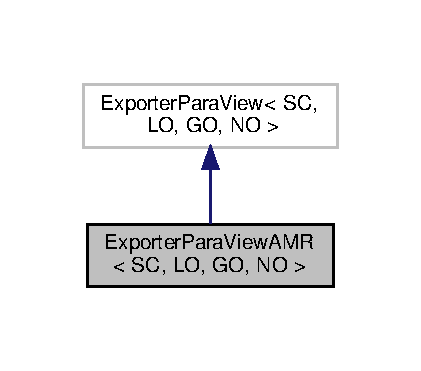
\includegraphics[width=202pt]{classFEDD_1_1ExporterParaViewAMR__inherit__graph}
\end{center}
\end{figure}


Collaboration diagram for Exporter\+Para\+View\+A\+MR$<$ SC, LO, GO, NO $>$\+:\nopagebreak
\begin{figure}[H]
\begin{center}
\leavevmode
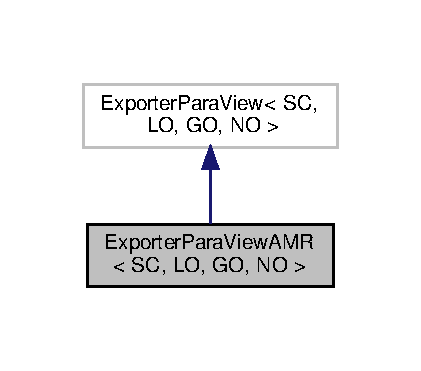
\includegraphics[width=202pt]{classFEDD_1_1ExporterParaViewAMR__coll__graph}
\end{center}
\end{figure}
\subsubsection*{Public Types}
\begin{DoxyCompactItemize}
\item 
\mbox{\Hypertarget{classFEDD_1_1ExporterParaViewAMR_ad857d990c6d8bcc423703888a1944171}\label{classFEDD_1_1ExporterParaViewAMR_ad857d990c6d8bcc423703888a1944171}} 
typedef std\+::vector$<$ double $>$ {\bfseries vec\+\_\+dbl}
\item 
\mbox{\Hypertarget{classFEDD_1_1ExporterParaViewAMR_a87c4014047e4914271a871d26324be53}\label{classFEDD_1_1ExporterParaViewAMR_a87c4014047e4914271a871d26324be53}} 
typedef std\+::vector$<$ std\+::vector$<$ double $>$ $>$ {\bfseries vec2\+D\+\_\+dbl}
\item 
\mbox{\Hypertarget{classFEDD_1_1ExporterParaViewAMR_a3f24281f52a42497ad16524768407426}\label{classFEDD_1_1ExporterParaViewAMR_a3f24281f52a42497ad16524768407426}} 
typedef std\+::vector$<$ std\+::vector$<$ int $>$ $>$ {\bfseries vec2\+D\+\_\+int}
\item 
\mbox{\Hypertarget{classFEDD_1_1ExporterParaViewAMR_aeb941029c519943fbbd78fa19617160b}\label{classFEDD_1_1ExporterParaViewAMR_aeb941029c519943fbbd78fa19617160b}} 
typedef std\+::vector$<$ std\+::vector$<$ long long $>$ $>$ {\bfseries vec2\+D\+\_\+longlong}
\item 
\mbox{\Hypertarget{classFEDD_1_1ExporterParaViewAMR_a3e13a99469a71351669c8db5b4b27652}\label{classFEDD_1_1ExporterParaViewAMR_a3e13a99469a71351669c8db5b4b27652}} 
typedef Teuchos\+::\+R\+CP$<$ std\+::vector$<$ int $>$ $>$ {\bfseries vec\+\_\+int\+\_\+ptr}
\item 
\mbox{\Hypertarget{classFEDD_1_1ExporterParaViewAMR_a2160534f29ad8e3030a39f191046d22c}\label{classFEDD_1_1ExporterParaViewAMR_a2160534f29ad8e3030a39f191046d22c}} 
typedef Teuchos\+::\+R\+CP$<$ std\+::vector$<$ long long $>$ $>$ {\bfseries vec\+\_\+longlong\+\_\+ptr}
\item 
\mbox{\Hypertarget{classFEDD_1_1ExporterParaViewAMR_a23051f635711fcea08566b941ae116d6}\label{classFEDD_1_1ExporterParaViewAMR_a23051f635711fcea08566b941ae116d6}} 
typedef Teuchos\+::\+R\+CP$<$ vec\+\_\+dbl $>$ {\bfseries vec\+\_\+dbl\+\_\+ptr}
\item 
\mbox{\Hypertarget{classFEDD_1_1ExporterParaViewAMR_ae1bcea1ccf798922bfe00746712617a4}\label{classFEDD_1_1ExporterParaViewAMR_ae1bcea1ccf798922bfe00746712617a4}} 
typedef Teuchos\+::\+R\+CP$<$ std\+::vector$<$ std\+::vector$<$ double $>$ $>$ $>$ {\bfseries vec2\+D\+\_\+dbl\+\_\+ptr}
\item 
\mbox{\Hypertarget{classFEDD_1_1ExporterParaViewAMR_a58f61f9bd3b700964b184e554e9e3478}\label{classFEDD_1_1ExporterParaViewAMR_a58f61f9bd3b700964b184e554e9e3478}} 
typedef Teuchos\+::\+R\+CP$<$ std\+::vector$<$ std\+::vector$<$ int $>$ $>$ $>$ {\bfseries vec2\+D\+\_\+int\+\_\+ptr}
\item 
\mbox{\Hypertarget{classFEDD_1_1ExporterParaViewAMR_a3246073b9e4717f898297922651a0b9e}\label{classFEDD_1_1ExporterParaViewAMR_a3246073b9e4717f898297922651a0b9e}} 
typedef Teuchos\+::\+R\+CP$<$ vec2\+D\+\_\+longlong $>$ {\bfseries vec2\+D\+\_\+longlong\+\_\+ptr}
\item 
\mbox{\Hypertarget{classFEDD_1_1ExporterParaViewAMR_acfb97ffe09d5b04085f9c0e2158662bf}\label{classFEDD_1_1ExporterParaViewAMR_acfb97ffe09d5b04085f9c0e2158662bf}} 
typedef Teuchos\+::\+R\+CP$<$ Epetra\+\_\+\+Vector $>$ {\bfseries Epetra\+Vec\+\_\+ptr}
\item 
\mbox{\Hypertarget{classFEDD_1_1ExporterParaViewAMR_a364814a2dc31b987778d984084bf2c36}\label{classFEDD_1_1ExporterParaViewAMR_a364814a2dc31b987778d984084bf2c36}} 
typedef Teuchos\+::\+R\+CP$<$ Epetra\+\_\+\+Mpi\+Comm $>$ {\bfseries Epetra\+Comm\+\_\+ptr}
\item 
\mbox{\Hypertarget{classFEDD_1_1ExporterParaViewAMR_a045884bf8773a282e771cae0ac4f6a5d}\label{classFEDD_1_1ExporterParaViewAMR_a045884bf8773a282e771cae0ac4f6a5d}} 
typedef Teuchos\+::\+R\+CP$<$ Epetra\+\_\+\+Int\+Vector $>$ {\bfseries Epetra\+Vec\+Int\+\_\+ptr}
\item 
\mbox{\Hypertarget{classFEDD_1_1ExporterParaViewAMR_af659f2e10e0d37bc8bf6d2197a4995d9}\label{classFEDD_1_1ExporterParaViewAMR_af659f2e10e0d37bc8bf6d2197a4995d9}} 
typedef Teuchos\+::\+R\+CP$<$ Epetra\+\_\+\+Long\+Long\+Vector $>$ {\bfseries Epetra\+Vec\+Long\+Long\+\_\+ptr}
\item 
\mbox{\Hypertarget{classFEDD_1_1ExporterParaViewAMR_acadc649fc9344c809da9d79cc727f77d}\label{classFEDD_1_1ExporterParaViewAMR_acadc649fc9344c809da9d79cc727f77d}} 
typedef Teuchos\+::\+R\+CP$<$ Epetra\+\_\+\+Multi\+Vector $>$ {\bfseries Epetra\+M\+V\+Ptr\+\_\+\+Type}
\item 
\mbox{\Hypertarget{classFEDD_1_1ExporterParaViewAMR_ae023113193df60c063f2d0c662c113a4}\label{classFEDD_1_1ExporterParaViewAMR_ae023113193df60c063f2d0c662c113a4}} 
typedef Teuchos\+::\+R\+CP$<$ Epetra\+\_\+\+Map $>$ {\bfseries Epetra\+Map\+Ptr\+\_\+\+Type}
\item 
\mbox{\Hypertarget{classFEDD_1_1ExporterParaViewAMR_aeb01b0bb15a52d67155d7799588af706}\label{classFEDD_1_1ExporterParaViewAMR_aeb01b0bb15a52d67155d7799588af706}} 
typedef Epetra\+Ext\+::\+H\+D\+F5 {\bfseries H\+D\+F5\+\_\+\+Type}
\item 
\mbox{\Hypertarget{classFEDD_1_1ExporterParaViewAMR_a0669ab1d36114d09d6ec07649e632b50}\label{classFEDD_1_1ExporterParaViewAMR_a0669ab1d36114d09d6ec07649e632b50}} 
typedef Teuchos\+::\+R\+CP$<$ H\+D\+F5\+\_\+\+Type $>$ {\bfseries H\+D\+F5\+Ptr\+\_\+\+Type}
\item 
\mbox{\Hypertarget{classFEDD_1_1ExporterParaViewAMR_a40f4b74a0cc62f2e9181c131fd31ce14}\label{classFEDD_1_1ExporterParaViewAMR_a40f4b74a0cc62f2e9181c131fd31ce14}} 
typedef Teuchos\+::\+Comm$<$ int $>$ {\bfseries Comm\+\_\+\+Type}
\item 
\mbox{\Hypertarget{classFEDD_1_1ExporterParaViewAMR_a1f3569403ac40bf19493e68a6667f40a}\label{classFEDD_1_1ExporterParaViewAMR_a1f3569403ac40bf19493e68a6667f40a}} 
typedef Teuchos\+::\+R\+CP$<$ const Comm\+\_\+\+Type $>$ {\bfseries Comm\+Const\+Ptr\+\_\+\+Type}
\item 
\mbox{\Hypertarget{classFEDD_1_1ExporterParaViewAMR_acdb41f657646474c2efb7f495f8725f7}\label{classFEDD_1_1ExporterParaViewAMR_acdb41f657646474c2efb7f495f8725f7}} 
typedef const Teuchos\+::\+R\+CP$<$ const Comm\+\_\+\+Type $>$ {\bfseries Comm\+Const\+Ptr\+Const\+\_\+\+Type}
\item 
\mbox{\Hypertarget{classFEDD_1_1ExporterParaViewAMR_a3c51bc6fe3a5ab13cd4e4fb44bff78c9}\label{classFEDD_1_1ExporterParaViewAMR_a3c51bc6fe3a5ab13cd4e4fb44bff78c9}} 
typedef Map$<$ LO, GO, NO $>$ {\bfseries Map\+\_\+\+Type}
\item 
\mbox{\Hypertarget{classFEDD_1_1ExporterParaViewAMR_af43e02540360a8c5acb334b2ce7d9c99}\label{classFEDD_1_1ExporterParaViewAMR_af43e02540360a8c5acb334b2ce7d9c99}} 
typedef Teuchos\+::\+R\+CP$<$ const Map\+\_\+\+Type $>$ {\bfseries Map\+Const\+Ptr\+\_\+\+Type}
\item 
\mbox{\Hypertarget{classFEDD_1_1ExporterParaViewAMR_a6550e2db4054f7535f9cb1758bb3397c}\label{classFEDD_1_1ExporterParaViewAMR_a6550e2db4054f7535f9cb1758bb3397c}} 
typedef const Map\+Const\+Ptr\+\_\+\+Type {\bfseries Map\+Const\+Ptr\+Const\+\_\+\+Type}
\item 
\mbox{\Hypertarget{classFEDD_1_1ExporterParaViewAMR_ae656c560626c10f5fc6722f43e4281fc}\label{classFEDD_1_1ExporterParaViewAMR_ae656c560626c10f5fc6722f43e4281fc}} 
typedef Multi\+Vector$<$ SC, LO, GO, NO $>$ {\bfseries Multi\+Vector\+\_\+\+Type}
\item 
\mbox{\Hypertarget{classFEDD_1_1ExporterParaViewAMR_a8caa4d56423da54bdfa117997252a400}\label{classFEDD_1_1ExporterParaViewAMR_a8caa4d56423da54bdfa117997252a400}} 
typedef Teuchos\+::\+R\+CP$<$ const Multi\+Vector\+\_\+\+Type $>$ {\bfseries Multi\+Vector\+Const\+Ptr\+\_\+\+Type}
\item 
\mbox{\Hypertarget{classFEDD_1_1ExporterParaViewAMR_a5c223e7593c38a53e11908ef7ee63a98}\label{classFEDD_1_1ExporterParaViewAMR_a5c223e7593c38a53e11908ef7ee63a98}} 
typedef const Multi\+Vector\+Const\+Ptr\+\_\+\+Type {\bfseries Multi\+Vector\+Const\+Ptr\+Const\+\_\+\+Type}
\item 
\mbox{\Hypertarget{classFEDD_1_1ExporterParaViewAMR_a1e469aabe3952e2cd5797236ba2d80b7}\label{classFEDD_1_1ExporterParaViewAMR_a1e469aabe3952e2cd5797236ba2d80b7}} 
typedef Mesh$<$ SC, LO, GO, NO $>$ {\bfseries Mesh\+\_\+\+Type}
\item 
\mbox{\Hypertarget{classFEDD_1_1ExporterParaViewAMR_a5e139c70ffeb95aaa46d5d2dc64e20c7}\label{classFEDD_1_1ExporterParaViewAMR_a5e139c70ffeb95aaa46d5d2dc64e20c7}} 
typedef Teuchos\+::\+R\+CP$<$ Mesh\+\_\+\+Type $>$ {\bfseries Mesh\+Ptr\+\_\+\+Type}
\item 
\mbox{\Hypertarget{classFEDD_1_1ExporterParaViewAMR_a6a376912bffdf1fcd740ffd7c6db719f}\label{classFEDD_1_1ExporterParaViewAMR_a6a376912bffdf1fcd740ffd7c6db719f}} 
typedef Mesh\+\_\+\+Type\+::\+Elements\+Ptr\+\_\+\+Type {\bfseries Elements\+Ptr\+\_\+\+Type}
\end{DoxyCompactItemize}
\subsubsection*{Public Member Functions}
\begin{DoxyCompactItemize}
\item 
\mbox{\Hypertarget{classFEDD_1_1ExporterParaViewAMR_a1c1672caa0d613c1d273089a9758f2ea}\label{classFEDD_1_1ExporterParaViewAMR_a1c1672caa0d613c1d273089a9758f2ea}} 
void {\bfseries update\+Variables} (Multi\+Vector\+Const\+Ptr\+\_\+\+Type \&u, std\+::string var\+Name)
\item 
\mbox{\Hypertarget{classFEDD_1_1ExporterParaViewAMR_a7147bdcbe93d3157b0717a82e8776ea5}\label{classFEDD_1_1ExporterParaViewAMR_a7147bdcbe93d3157b0717a82e8776ea5}} 
void {\bfseries re\+Setup} (Mesh\+Ptr\+\_\+\+Type mesh)
\end{DoxyCompactItemize}


The documentation for this class was generated from the following files\+:\begin{DoxyCompactItemize}
\item 
Exporter\+Para\+View\+A\+M\+R\+\_\+decl.\+hpp\item 
Exporter\+Para\+View\+A\+M\+R\+\_\+def.\+hpp\end{DoxyCompactItemize}

\hypertarget{classFEDD_1_1RefinementFactory}{}\section{F\+E\+DD\+:\+:Refinement\+Factory$<$ SC, LO, GO, NO $>$ Class Template Reference}
\label{classFEDD_1_1RefinementFactory}\index{F\+E\+D\+D\+::\+Refinement\+Factory$<$ S\+C, L\+O, G\+O, N\+O $>$@{F\+E\+D\+D\+::\+Refinement\+Factory$<$ S\+C, L\+O, G\+O, N\+O $>$}}


{\ttfamily \#include $<$Refinement\+Factory\+\_\+decl.\+hpp$>$}



Inheritance diagram for F\+E\+DD\+:\+:Refinement\+Factory$<$ SC, LO, GO, NO $>$\+:\nopagebreak
\begin{figure}[H]
\begin{center}
\leavevmode
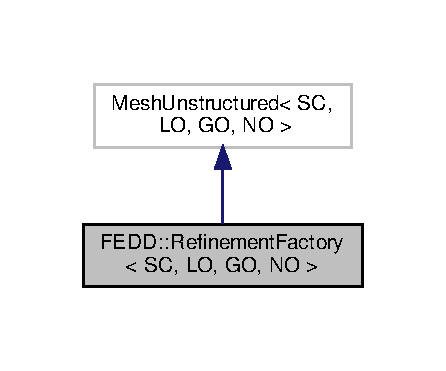
\includegraphics[width=214pt]{classFEDD_1_1RefinementFactory__inherit__graph}
\end{center}
\end{figure}


Collaboration diagram for F\+E\+DD\+:\+:Refinement\+Factory$<$ SC, LO, GO, NO $>$\+:\nopagebreak
\begin{figure}[H]
\begin{center}
\leavevmode
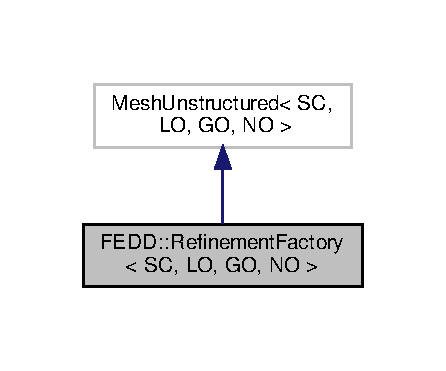
\includegraphics[width=214pt]{classFEDD_1_1RefinementFactory__coll__graph}
\end{center}
\end{figure}
\subsection*{Public Types}
\begin{DoxyCompactItemize}
\item 
typedef Mesh$<$ SC, LO, GO, NO $>$ \hyperlink{classFEDD_1_1RefinementFactory_a19f6ea9d9d873657041004fa12f76ac5}{Mesh\+\_\+\+Type}
\item 
typedef Teuchos\+::\+R\+CP$<$ Mesh\+Unstructured$<$ SC, LO, GO, NO $>$ $>$ \hyperlink{classFEDD_1_1RefinementFactory_a1a278d01c278972af01f2996247af8ac}{Mesh\+Unstr\+Ptr\+\_\+\+Type}
\item 
typedef std\+::vector$<$ \hyperlink{classFEDD_1_1RefinementFactory_a1a278d01c278972af01f2996247af8ac}{Mesh\+Unstr\+Ptr\+\_\+\+Type} $>$ \hyperlink{classFEDD_1_1RefinementFactory_a772a738296d703be721b9b1c877f1a9e}{Mesh\+Unstr\+Ptr\+Array\+\_\+\+Type}
\item 
typedef Mesh\+Unstructured\+Refinement$<$ SC, LO, GO, NO $>$ \hyperlink{classFEDD_1_1RefinementFactory_a22aea92d236fb822fef9557c22834062}{Mesh\+Unstr\+Ref\+\_\+\+Type}
\item 
typedef Teuchos\+::\+R\+CP$<$ \hyperlink{classFEDD_1_1RefinementFactory_a22aea92d236fb822fef9557c22834062}{Mesh\+Unstr\+Ref\+\_\+\+Type} $>$ \hyperlink{classFEDD_1_1RefinementFactory_aea0fab96821387bc772333299102b2c9}{Mesh\+Unstr\+Ref\+Ptr\+\_\+\+Type}
\item 
typedef std\+::vector$<$ \hyperlink{classFEDD_1_1RefinementFactory_aea0fab96821387bc772333299102b2c9}{Mesh\+Unstr\+Ref\+Ptr\+\_\+\+Type} $>$ \hyperlink{classFEDD_1_1RefinementFactory_af6e25bbcc6f5e8d6ee70a1c5aab1e3eb}{Mesh\+Unstr\+Ref\+Ptr\+Array\+\_\+\+Type}
\item 
typedef Mesh\+\_\+\+Type\+::\+Comm\+Ptr\+\_\+\+Type \hyperlink{classFEDD_1_1RefinementFactory_ad2163b2c380d83b6b28a695f6f8e8a56}{Comm\+Ptr\+\_\+\+Type}
\item 
typedef Mesh\+\_\+\+Type\+::\+Comm\+Const\+Ptr\+\_\+\+Type \hyperlink{classFEDD_1_1RefinementFactory_a58381e0786c65ec61d11bc73c224b45a}{Comm\+Const\+Ptr\+\_\+\+Type}
\item 
typedef Elements \hyperlink{classFEDD_1_1RefinementFactory_a0879b04ac1b1830fae7d6a7e29d36000}{Elements\+\_\+\+Type}
\item 
typedef Teuchos\+::\+R\+CP$<$ \hyperlink{classFEDD_1_1RefinementFactory_a0879b04ac1b1830fae7d6a7e29d36000}{Elements\+\_\+\+Type} $>$ \hyperlink{classFEDD_1_1RefinementFactory_a0994b5b7b6d080048673941251999f2e}{Elements\+Ptr\+\_\+\+Type}
\item 
typedef Surface\+Elements \hyperlink{classFEDD_1_1RefinementFactory_ac050bc27156fc5a1e8bf0e01381c33c4}{Surface\+Elements\+\_\+\+Type}
\item 
typedef Teuchos\+::\+R\+CP$<$ \hyperlink{classFEDD_1_1RefinementFactory_ac050bc27156fc5a1e8bf0e01381c33c4}{Surface\+Elements\+\_\+\+Type} $>$ \hyperlink{classFEDD_1_1RefinementFactory_a1067ba23325b19eae16a864f25f7d68f}{Surface\+Elements\+Ptr\+\_\+\+Type}
\item 
typedef Edge\+Elements \hyperlink{classFEDD_1_1RefinementFactory_a11b30196ff403358f3540117f09b6963}{Edge\+Elements\+\_\+\+Type}
\item 
typedef Teuchos\+::\+R\+CP$<$ \hyperlink{classFEDD_1_1RefinementFactory_a11b30196ff403358f3540117f09b6963}{Edge\+Elements\+\_\+\+Type} $>$ \hyperlink{classFEDD_1_1RefinementFactory_ae5285e990ec4632d6188a1280627ad13}{Edge\+Elements\+Ptr\+\_\+\+Type}
\item 
typedef Mesh\+Interface$<$ SC, LO, GO, NO $>$ \hyperlink{classFEDD_1_1RefinementFactory_aff8bb4cd3896a419c36d4baabccbf28a}{Mesh\+Interface\+\_\+\+Type}
\item 
typedef Teuchos\+::\+R\+CP$<$ \hyperlink{classFEDD_1_1RefinementFactory_aff8bb4cd3896a419c36d4baabccbf28a}{Mesh\+Interface\+\_\+\+Type} $>$ \hyperlink{classFEDD_1_1RefinementFactory_a2217802fcbb1342b135d33ea70411089}{Mesh\+Interface\+Ptr\+\_\+\+Type}
\item 
typedef Map$<$ LO, GO, NO $>$ \hyperlink{classFEDD_1_1RefinementFactory_ae3b9a462f8534ab43ce0dbf0d44b3bc5}{Map\+\_\+\+Type}
\item 
typedef Map\+\_\+\+Type\+::\+Map\+Ptr\+\_\+\+Type \hyperlink{classFEDD_1_1RefinementFactory_a554f7a4c5f5014e2ddec03a2e667016c}{Map\+Ptr\+\_\+\+Type}
\item 
typedef Map\+\_\+\+Type\+::\+Map\+Const\+Ptr\+\_\+\+Type \hyperlink{classFEDD_1_1RefinementFactory_a8256ccdf1b2a5c977ddc011f4e8eb8d3}{Map\+Const\+Ptr\+\_\+\+Type}
\item 
typedef Multi\+Vector$<$ SC, LO, GO, NO $>$ \hyperlink{classFEDD_1_1RefinementFactory_af7c4cb285d95e61820d63b9344a90976}{Multi\+Vector\+\_\+\+Type}
\item 
typedef Teuchos\+::\+R\+CP$<$ \hyperlink{classFEDD_1_1RefinementFactory_af7c4cb285d95e61820d63b9344a90976}{Multi\+Vector\+\_\+\+Type} $>$ \hyperlink{classFEDD_1_1RefinementFactory_a0592bb145b1f5b1daac2e69a96c23cb5}{Multi\+Vector\+Ptr\+\_\+\+Type}
\item 
typedef Multi\+Vector$<$ LO, LO, GO, NO $>$ \hyperlink{classFEDD_1_1RefinementFactory_ae731f05f6a28d13f917230f914f29037}{Multi\+Vector\+L\+O\+\_\+\+Type}
\item 
typedef Teuchos\+::\+R\+CP$<$ \hyperlink{classFEDD_1_1RefinementFactory_ae731f05f6a28d13f917230f914f29037}{Multi\+Vector\+L\+O\+\_\+\+Type} $>$ \hyperlink{classFEDD_1_1RefinementFactory_a002c7179ca2f22db4505da2db0f798e9}{Multi\+Vector\+L\+O\+Ptr\+\_\+\+Type}
\item 
typedef Multi\+Vector$<$ GO, LO, GO, NO $>$ \hyperlink{classFEDD_1_1RefinementFactory_a433fd79c1903a3771cffbaed6f5dbd71}{Multi\+Vector\+G\+O\+\_\+\+Type}
\item 
typedef Teuchos\+::\+R\+CP$<$ \hyperlink{classFEDD_1_1RefinementFactory_a433fd79c1903a3771cffbaed6f5dbd71}{Multi\+Vector\+G\+O\+\_\+\+Type} $>$ \hyperlink{classFEDD_1_1RefinementFactory_a9e4318c3bc9a63b25f6283955ff80d49}{Multi\+Vector\+G\+O\+Ptr\+\_\+\+Type}
\item 
typedef Teuchos\+::\+R\+CP$<$ const \hyperlink{classFEDD_1_1RefinementFactory_af7c4cb285d95e61820d63b9344a90976}{Multi\+Vector\+\_\+\+Type} $>$ \hyperlink{classFEDD_1_1RefinementFactory_af904cdbfa726de22dcea9dfcc891114b}{Multi\+Vector\+Ptr\+Const\+\_\+\+Type}
\item 
typedef Teuchos\+::\+Ordinal\+Traits$<$ LO $>$ \hyperlink{classFEDD_1_1RefinementFactory_a266b4b5a15cabb39df492db6e4f53e3e}{O\+T\+LO}
\item 
typedef Matrix$<$ SC, LO, GO, NO $>$ \hyperlink{classFEDD_1_1RefinementFactory_ab04c3bb37b70c0524f46b050aaec1914}{Matrix\+\_\+\+Type}
\item 
typedef Teuchos\+::\+R\+CP$<$ \hyperlink{classFEDD_1_1RefinementFactory_ab04c3bb37b70c0524f46b050aaec1914}{Matrix\+\_\+\+Type} $>$ \hyperlink{classFEDD_1_1RefinementFactory_a52d5a6625f207bc4df2c5ae3362e8ced}{Matrix\+Ptr\+\_\+\+Type}
\item 
typedef Exporter\+Para\+View$<$ SC, LO, GO, NO $>$ \hyperlink{classFEDD_1_1RefinementFactory_a268cb28ca6c68a4c32a912068c643933}{Exporter\+\_\+\+Type}
\item 
typedef Teuchos\+::\+R\+CP$<$ \hyperlink{classFEDD_1_1RefinementFactory_a268cb28ca6c68a4c32a912068c643933}{Exporter\+\_\+\+Type} $>$ \hyperlink{classFEDD_1_1RefinementFactory_ae74a8143ddf273f2a13df4055233759c}{Exporter\+Ptr\+\_\+\+Type}
\item 
typedef Teuchos\+::\+R\+CP$<$ Exporter\+Txt $>$ \hyperlink{classFEDD_1_1RefinementFactory_a08c0a0d5b375af33c924f90005302f91}{Exporter\+Txt\+Ptr\+\_\+\+Type}
\end{DoxyCompactItemize}
\subsection*{Public Member Functions}
\begin{DoxyCompactItemize}
\item 
\hyperlink{classFEDD_1_1RefinementFactory_a45a83da1b5be5f4bcb091cf56caca25e}{Refinement\+Factory} ()
\item 
\hyperlink{classFEDD_1_1RefinementFactory_a0815e8208b193e64c26e64d94691a967}{Refinement\+Factory} (\hyperlink{classFEDD_1_1RefinementFactory_a58381e0786c65ec61d11bc73c224b45a}{Comm\+Const\+Ptr\+\_\+\+Type} comm, int volume\+ID=10)
\item 
\hyperlink{classFEDD_1_1RefinementFactory_a59e3730c7f4ee1769e34da85250d0d86}{Refinement\+Factory} (\hyperlink{classFEDD_1_1RefinementFactory_a58381e0786c65ec61d11bc73c224b45a}{Comm\+Const\+Ptr\+\_\+\+Type} comm, int volume\+ID, \hyperlink{classFEDD_1_1RefinementFactory_a1a278d01c278972af01f2996247af8ac}{Mesh\+Unstr\+Ptr\+\_\+\+Type} mesh\+P1)
\item 
\hyperlink{classFEDD_1_1RefinementFactory_ae9b8ba9b12e35db03ef1b6363c1b9200}{$\sim$\+Refinement\+Factory} ()
\item 
void \hyperlink{classFEDD_1_1RefinementFactory_aec49fcc71406ba48eb7d6766653914d5}{refine\+Mesh} (\hyperlink{classFEDD_1_1RefinementFactory_af6e25bbcc6f5e8d6ee70a1c5aab1e3eb}{Mesh\+Unstr\+Ref\+Ptr\+Array\+\_\+\+Type} mesh\+P1, int iteration)
\item 
void \hyperlink{classFEDD_1_1RefinementFactory_af7a24f2ea3ebe601eb6359b1b0bbc9a7}{assign\+Edge\+Flags} (\hyperlink{classFEDD_1_1RefinementFactory_aea0fab96821387bc772333299102b2c9}{Mesh\+Unstr\+Ref\+Ptr\+\_\+\+Type} mesh\+P1, \hyperlink{classFEDD_1_1RefinementFactory_ae5285e990ec4632d6188a1280627ad13}{Edge\+Elements\+Ptr\+\_\+\+Type} edge\+Elements)
\item 
void \hyperlink{classFEDD_1_1RefinementFactory_a530ccd6a31c259515ab1900d544eb813}{refine\+Regular} (\hyperlink{classFEDD_1_1RefinementFactory_ae5285e990ec4632d6188a1280627ad13}{Edge\+Elements\+Ptr\+\_\+\+Type} edge\+Elements, \hyperlink{classFEDD_1_1RefinementFactory_a0994b5b7b6d080048673941251999f2e}{Elements\+Ptr\+\_\+\+Type} elements, int i)
\item 
void \hyperlink{classFEDD_1_1RefinementFactory_a130f21212d5edaad2dc8f809a2628f2a}{refine\+Green} (\hyperlink{classFEDD_1_1RefinementFactory_ae5285e990ec4632d6188a1280627ad13}{Edge\+Elements\+Ptr\+\_\+\+Type} edge\+Elements, \hyperlink{classFEDD_1_1RefinementFactory_a0994b5b7b6d080048673941251999f2e}{Elements\+Ptr\+\_\+\+Type} elements, int i)
\item 
void \hyperlink{classFEDD_1_1RefinementFactory_aeeebbc6bfb22dfb14470cf628400733a}{refine\+Blue} (\hyperlink{classFEDD_1_1RefinementFactory_ae5285e990ec4632d6188a1280627ad13}{Edge\+Elements\+Ptr\+\_\+\+Type} edge\+Elements, \hyperlink{classFEDD_1_1RefinementFactory_a0994b5b7b6d080048673941251999f2e}{Elements\+Ptr\+\_\+\+Type} elements, int i)
\item 
void \hyperlink{classFEDD_1_1RefinementFactory_ad8bc07f5d6bfe7f7180bd32d7cc4ea0c}{refine\+Red} (\hyperlink{classFEDD_1_1RefinementFactory_ae5285e990ec4632d6188a1280627ad13}{Edge\+Elements\+Ptr\+\_\+\+Type} edge\+Elements, \hyperlink{classFEDD_1_1RefinementFactory_a0994b5b7b6d080048673941251999f2e}{Elements\+Ptr\+\_\+\+Type} elements, int i)
\item 
void \hyperlink{classFEDD_1_1RefinementFactory_a89b2f7d45585b804e32b278b83954153}{refine\+Type1} (\hyperlink{classFEDD_1_1RefinementFactory_ae5285e990ec4632d6188a1280627ad13}{Edge\+Elements\+Ptr\+\_\+\+Type} edge\+Elements, \hyperlink{classFEDD_1_1RefinementFactory_a0994b5b7b6d080048673941251999f2e}{Elements\+Ptr\+\_\+\+Type} elements, int index\+Element)
\item 
void \hyperlink{classFEDD_1_1RefinementFactory_ac43c76ce4137963ac5aac1355d38dbac}{refine\+Type2} (\hyperlink{classFEDD_1_1RefinementFactory_ae5285e990ec4632d6188a1280627ad13}{Edge\+Elements\+Ptr\+\_\+\+Type} edge\+Elements, \hyperlink{classFEDD_1_1RefinementFactory_a0994b5b7b6d080048673941251999f2e}{Elements\+Ptr\+\_\+\+Type} elements, int index\+Element)
\item 
void \hyperlink{classFEDD_1_1RefinementFactory_a282ee48e155d2f3f0e0a3faa0fa275d2}{refine\+Type3} (\hyperlink{classFEDD_1_1RefinementFactory_ae5285e990ec4632d6188a1280627ad13}{Edge\+Elements\+Ptr\+\_\+\+Type} edge\+Elements, \hyperlink{classFEDD_1_1RefinementFactory_a0994b5b7b6d080048673941251999f2e}{Elements\+Ptr\+\_\+\+Type} elements, int index\+Element)
\item 
void \hyperlink{classFEDD_1_1RefinementFactory_acb0db07f3517256e51e05380467c9782}{refine\+Type4} (\hyperlink{classFEDD_1_1RefinementFactory_ae5285e990ec4632d6188a1280627ad13}{Edge\+Elements\+Ptr\+\_\+\+Type} edge\+Elements, \hyperlink{classFEDD_1_1RefinementFactory_a0994b5b7b6d080048673941251999f2e}{Elements\+Ptr\+\_\+\+Type} elements, int index\+Element)
\item 
void \hyperlink{classFEDD_1_1RefinementFactory_af40b1acc9353be1408fed4d6a61ed2ae}{add\+Midpoint} (\hyperlink{classFEDD_1_1RefinementFactory_ae5285e990ec4632d6188a1280627ad13}{Edge\+Elements\+Ptr\+\_\+\+Type} edge\+Elements, int i)
\item 
int \hyperlink{classFEDD_1_1RefinementFactory_a383adbeffceada793b6805fb02fa5568}{determine\+Longest\+Edge} (\hyperlink{classFEDD_1_1RefinementFactory_ae5285e990ec4632d6188a1280627ad13}{Edge\+Elements\+Ptr\+\_\+\+Type} edge\+Elements, vec\+\_\+int\+\_\+\+Type edge\+Vec, vec2\+D\+\_\+dbl\+\_\+ptr\+\_\+\+Type points)
\item 
void \hyperlink{classFEDD_1_1RefinementFactory_a4294d0901e6691203b9043bb2f9c6ac6}{build\+Edge\+Map} (\hyperlink{classFEDD_1_1RefinementFactory_a8256ccdf1b2a5c977ddc011f4e8eb8d3}{Map\+Const\+Ptr\+\_\+\+Type} map\+Global\+Proc, \hyperlink{classFEDD_1_1RefinementFactory_a8256ccdf1b2a5c977ddc011f4e8eb8d3}{Map\+Const\+Ptr\+\_\+\+Type} map\+Proc)
\item 
void \hyperlink{classFEDD_1_1RefinementFactory_abeca9755a1bd393c36c792a78c6779e9}{build\+Node\+Map} (\hyperlink{classFEDD_1_1RefinementFactory_ae5285e990ec4632d6188a1280627ad13}{Edge\+Elements\+Ptr\+\_\+\+Type} edge\+Elements, \hyperlink{classFEDD_1_1RefinementFactory_a8256ccdf1b2a5c977ddc011f4e8eb8d3}{Map\+Const\+Ptr\+\_\+\+Type} map\+Global\+Proc, \hyperlink{classFEDD_1_1RefinementFactory_a8256ccdf1b2a5c977ddc011f4e8eb8d3}{Map\+Const\+Ptr\+\_\+\+Type} map\+Proc, int new\+Points, int new\+Points\+Repeated)
\item 
void \hyperlink{classFEDD_1_1RefinementFactory_a39c950be5d386f7a75f6d7392a9a2bc8}{build\+Triangle\+Map} ()
\item 
void \hyperlink{classFEDD_1_1RefinementFactory_a2ebf82a5deb92e26a48805fd470f6840}{update\+Elements\+Of\+Edges\+Local\+And\+Global} (int max\+Rank, \hyperlink{classFEDD_1_1RefinementFactory_a8256ccdf1b2a5c977ddc011f4e8eb8d3}{Map\+Const\+Ptr\+\_\+\+Type} edge\+Map)
\item 
void \hyperlink{classFEDD_1_1RefinementFactory_a8f295b405de2c056298b695bea51887b}{update\+Elements\+Of\+Surface\+Local\+And\+Global} (\hyperlink{classFEDD_1_1RefinementFactory_ae5285e990ec4632d6188a1280627ad13}{Edge\+Elements\+Ptr\+\_\+\+Type} edge\+Elements)
\item 
vec\+\_\+bool\+\_\+\+Type \hyperlink{classFEDD_1_1RefinementFactory_a97003a4445b40ac91728639de432a449}{check\+Interface\+Surface} (\hyperlink{classFEDD_1_1RefinementFactory_ae5285e990ec4632d6188a1280627ad13}{Edge\+Elements\+Ptr\+\_\+\+Type} edge\+Elements, vec\+\_\+int\+\_\+\+Type origin\+Flag, vec\+\_\+int\+\_\+\+Type edge\+Numbers, int index\+Element)
\item 
void \hyperlink{classFEDD_1_1RefinementFactory_a8f76b86ec161e405857e5c4a51aea968}{tag\+Area} (vec2\+D\+\_\+dbl\+\_\+\+Type area)
\item 
void \hyperlink{classFEDD_1_1RefinementFactory_a7099db47add1a0f9e431fc960860db2d}{refinement\+Restrictions} (\hyperlink{classFEDD_1_1RefinementFactory_aea0fab96821387bc772333299102b2c9}{Mesh\+Unstr\+Ref\+Ptr\+\_\+\+Type} mesh\+P1, \hyperlink{classFEDD_1_1RefinementFactory_a0994b5b7b6d080048673941251999f2e}{Elements\+Ptr\+\_\+\+Type} elements, \hyperlink{classFEDD_1_1RefinementFactory_ae5285e990ec4632d6188a1280627ad13}{Edge\+Elements\+Ptr\+\_\+\+Type} edge\+Elements, int iteration, int \&new\+Points, int \&new\+Points\+Common, vec\+\_\+\+G\+O\+\_\+\+Type \&global\+Interface\+I\+Ds\+Tagged, \hyperlink{classFEDD_1_1RefinementFactory_a8256ccdf1b2a5c977ddc011f4e8eb8d3}{Map\+Const\+Ptr\+\_\+\+Type} map\+Interface\+Edges, string restriction, int \&new\+Elements)
\item 
void \hyperlink{classFEDD_1_1RefinementFactory_ae4401ece866b918923322d46d0c5e33e}{refine\+Irregular} (\hyperlink{classFEDD_1_1RefinementFactory_a0994b5b7b6d080048673941251999f2e}{Elements\+Ptr\+\_\+\+Type} elements, \hyperlink{classFEDD_1_1RefinementFactory_ae5285e990ec4632d6188a1280627ad13}{Edge\+Elements\+Ptr\+\_\+\+Type} edge\+Elements, int \&new\+Elements, \hyperlink{classFEDD_1_1RefinementFactory_a8256ccdf1b2a5c977ddc011f4e8eb8d3}{Map\+Const\+Ptr\+\_\+\+Type} edge\+Map, \hyperlink{classFEDD_1_1RefinementFactory_a1067ba23325b19eae16a864f25f7d68f}{Surface\+Elements\+Ptr\+\_\+\+Type} surface\+Triangle\+Elements)
\item 
void \hyperlink{classFEDD_1_1RefinementFactory_acc422779a3cf6ca5a4c916acf7708418}{build\+Surface\+Triangle\+Elements} (\hyperlink{classFEDD_1_1RefinementFactory_a0994b5b7b6d080048673941251999f2e}{Elements\+Ptr\+\_\+\+Type} elements, \hyperlink{classFEDD_1_1RefinementFactory_ae5285e990ec4632d6188a1280627ad13}{Edge\+Elements\+Ptr\+\_\+\+Type} edge\+Elements)
\item 
void \hyperlink{classFEDD_1_1RefinementFactory_a4532ed5c403d767f316e922a3d769853}{set\+Error\+Estimate} (vec\+\_\+dbl\+\_\+\+Type error\+Elements)
\item 
vec\+\_\+dbl\+\_\+\+Type \hyperlink{classFEDD_1_1RefinementFactory_aecc0c9142abed8227daa43fc5db6ae1c}{get\+Error\+Estimate} ()
\end{DoxyCompactItemize}
\subsection*{Data Fields}
\begin{DoxyCompactItemize}
\item 
string \hyperlink{classFEDD_1_1RefinementFactory_a2dda98963313023311f044d248befd40}{refinement\+Restriction\+\_\+} = \char`\"{}none\char`\"{}
\item 
string \hyperlink{classFEDD_1_1RefinementFactory_aa499fe1f4daaed1c19fd1744d73c3706}{marking\+Strategy\+\_\+} = \char`\"{}Maximum\char`\"{}
\item 
double \hyperlink{classFEDD_1_1RefinementFactory_aac84121e72b1c2c6ff1691dc91acc9b1}{theta\+\_\+} = 0.\+5
\item 
bool \hyperlink{classFEDD_1_1RefinementFactory_a74d0dd46b30f83f868cd749d28375a42}{mesh\+Quality\+Print\+\_\+} = \char`\"{}false\char`\"{}
\item 
bool \hyperlink{classFEDD_1_1RefinementFactory_ad7ff86aebffde685089d462f2d04203e}{time\+Table\+Print\+\_\+} = \char`\"{}false\char`\"{}
\item 
int \hyperlink{classFEDD_1_1RefinementFactory_a7466053f06c1d52d6fb2c58db06b7a71}{refinement3\+D\+Diagonal\+\_\+} = 0
\end{DoxyCompactItemize}
\subsection*{Protected Attributes}
\begin{DoxyCompactItemize}
\item 
vec\+\_\+\+G\+O\+\_\+\+Type \hyperlink{classFEDD_1_1RefinementFactory_ae71ae7a6d0586a37cdc2aadfafeb00c4}{global\+Interface\+I\+Ds\+\_\+}
\item 
vec\+\_\+dbl\+\_\+\+Type \hyperlink{classFEDD_1_1RefinementFactory_ae04f877455828ca9d2328b6b29a72652}{error\+Estimation\+\_\+}
\item 
vec\+\_\+dbl\+\_\+\+Type \hyperlink{classFEDD_1_1RefinementFactory_ac8f78b4bd97729d0ca0a3a36097da107}{area\+Triangles\+\_\+}
\item 
vec\+\_\+dbl\+\_\+\+Type \hyperlink{classFEDD_1_1RefinementFactory_a7043a525164368b18359a399dede06c3}{vol\+Tetraeders\+\_\+}
\item 
vec\+\_\+dbl\+\_\+\+Type \hyperlink{classFEDD_1_1RefinementFactory_ad1c44661ff740905f2b3634ea285e1a7}{h\+\_\+\+T\+\_\+diam\+\_\+\+E\+\_\+}
\item 
vec\+\_\+dbl\+\_\+\+Type \hyperlink{classFEDD_1_1RefinementFactory_add2c3dc6ee30afaf225baed853475e06}{h\+\_\+\+T\+\_\+min\+\_\+}
\item 
\hyperlink{classFEDD_1_1RefinementFactory_a8256ccdf1b2a5c977ddc011f4e8eb8d3}{Map\+Const\+Ptr\+\_\+\+Type} \hyperlink{classFEDD_1_1RefinementFactory_ae21de28f0848c556b0c90cf6f912de25}{surface\+Triangle\+Map\+\_\+}
\end{DoxyCompactItemize}


\subsection{Member Typedef Documentation}
\mbox{\Hypertarget{classFEDD_1_1RefinementFactory_a58381e0786c65ec61d11bc73c224b45a}\label{classFEDD_1_1RefinementFactory_a58381e0786c65ec61d11bc73c224b45a}} 
\index{F\+E\+D\+D\+::\+Refinement\+Factory@{F\+E\+D\+D\+::\+Refinement\+Factory}!Comm\+Const\+Ptr\+\_\+\+Type@{Comm\+Const\+Ptr\+\_\+\+Type}}
\index{Comm\+Const\+Ptr\+\_\+\+Type@{Comm\+Const\+Ptr\+\_\+\+Type}!F\+E\+D\+D\+::\+Refinement\+Factory@{F\+E\+D\+D\+::\+Refinement\+Factory}}
\subsubsection{\texorpdfstring{Comm\+Const\+Ptr\+\_\+\+Type}{CommConstPtr\_Type}}
{\footnotesize\ttfamily template$<$class SC  = default\+\_\+sc, class LO  = default\+\_\+lo, class GO  = default\+\_\+go, class NO  = default\+\_\+no$>$ \\
typedef Mesh\+\_\+\+Type\+::\+Comm\+Const\+Ptr\+\_\+\+Type \hyperlink{classFEDD_1_1RefinementFactory}{F\+E\+D\+D\+::\+Refinement\+Factory}$<$ SC, LO, GO, NO $>$\+::\hyperlink{classFEDD_1_1RefinementFactory_a58381e0786c65ec61d11bc73c224b45a}{Comm\+Const\+Ptr\+\_\+\+Type}}

\mbox{\Hypertarget{classFEDD_1_1RefinementFactory_ad2163b2c380d83b6b28a695f6f8e8a56}\label{classFEDD_1_1RefinementFactory_ad2163b2c380d83b6b28a695f6f8e8a56}} 
\index{F\+E\+D\+D\+::\+Refinement\+Factory@{F\+E\+D\+D\+::\+Refinement\+Factory}!Comm\+Ptr\+\_\+\+Type@{Comm\+Ptr\+\_\+\+Type}}
\index{Comm\+Ptr\+\_\+\+Type@{Comm\+Ptr\+\_\+\+Type}!F\+E\+D\+D\+::\+Refinement\+Factory@{F\+E\+D\+D\+::\+Refinement\+Factory}}
\subsubsection{\texorpdfstring{Comm\+Ptr\+\_\+\+Type}{CommPtr\_Type}}
{\footnotesize\ttfamily template$<$class SC  = default\+\_\+sc, class LO  = default\+\_\+lo, class GO  = default\+\_\+go, class NO  = default\+\_\+no$>$ \\
typedef Mesh\+\_\+\+Type\+::\+Comm\+Ptr\+\_\+\+Type \hyperlink{classFEDD_1_1RefinementFactory}{F\+E\+D\+D\+::\+Refinement\+Factory}$<$ SC, LO, GO, NO $>$\+::\hyperlink{classFEDD_1_1RefinementFactory_ad2163b2c380d83b6b28a695f6f8e8a56}{Comm\+Ptr\+\_\+\+Type}}

\mbox{\Hypertarget{classFEDD_1_1RefinementFactory_a11b30196ff403358f3540117f09b6963}\label{classFEDD_1_1RefinementFactory_a11b30196ff403358f3540117f09b6963}} 
\index{F\+E\+D\+D\+::\+Refinement\+Factory@{F\+E\+D\+D\+::\+Refinement\+Factory}!Edge\+Elements\+\_\+\+Type@{Edge\+Elements\+\_\+\+Type}}
\index{Edge\+Elements\+\_\+\+Type@{Edge\+Elements\+\_\+\+Type}!F\+E\+D\+D\+::\+Refinement\+Factory@{F\+E\+D\+D\+::\+Refinement\+Factory}}
\subsubsection{\texorpdfstring{Edge\+Elements\+\_\+\+Type}{EdgeElements\_Type}}
{\footnotesize\ttfamily template$<$class SC  = default\+\_\+sc, class LO  = default\+\_\+lo, class GO  = default\+\_\+go, class NO  = default\+\_\+no$>$ \\
typedef Edge\+Elements \hyperlink{classFEDD_1_1RefinementFactory}{F\+E\+D\+D\+::\+Refinement\+Factory}$<$ SC, LO, GO, NO $>$\+::\hyperlink{classFEDD_1_1RefinementFactory_a11b30196ff403358f3540117f09b6963}{Edge\+Elements\+\_\+\+Type}}

\mbox{\Hypertarget{classFEDD_1_1RefinementFactory_ae5285e990ec4632d6188a1280627ad13}\label{classFEDD_1_1RefinementFactory_ae5285e990ec4632d6188a1280627ad13}} 
\index{F\+E\+D\+D\+::\+Refinement\+Factory@{F\+E\+D\+D\+::\+Refinement\+Factory}!Edge\+Elements\+Ptr\+\_\+\+Type@{Edge\+Elements\+Ptr\+\_\+\+Type}}
\index{Edge\+Elements\+Ptr\+\_\+\+Type@{Edge\+Elements\+Ptr\+\_\+\+Type}!F\+E\+D\+D\+::\+Refinement\+Factory@{F\+E\+D\+D\+::\+Refinement\+Factory}}
\subsubsection{\texorpdfstring{Edge\+Elements\+Ptr\+\_\+\+Type}{EdgeElementsPtr\_Type}}
{\footnotesize\ttfamily template$<$class SC  = default\+\_\+sc, class LO  = default\+\_\+lo, class GO  = default\+\_\+go, class NO  = default\+\_\+no$>$ \\
typedef Teuchos\+::\+R\+CP$<$\hyperlink{classFEDD_1_1RefinementFactory_a11b30196ff403358f3540117f09b6963}{Edge\+Elements\+\_\+\+Type}$>$ \hyperlink{classFEDD_1_1RefinementFactory}{F\+E\+D\+D\+::\+Refinement\+Factory}$<$ SC, LO, GO, NO $>$\+::\hyperlink{classFEDD_1_1RefinementFactory_ae5285e990ec4632d6188a1280627ad13}{Edge\+Elements\+Ptr\+\_\+\+Type}}

\mbox{\Hypertarget{classFEDD_1_1RefinementFactory_a0879b04ac1b1830fae7d6a7e29d36000}\label{classFEDD_1_1RefinementFactory_a0879b04ac1b1830fae7d6a7e29d36000}} 
\index{F\+E\+D\+D\+::\+Refinement\+Factory@{F\+E\+D\+D\+::\+Refinement\+Factory}!Elements\+\_\+\+Type@{Elements\+\_\+\+Type}}
\index{Elements\+\_\+\+Type@{Elements\+\_\+\+Type}!F\+E\+D\+D\+::\+Refinement\+Factory@{F\+E\+D\+D\+::\+Refinement\+Factory}}
\subsubsection{\texorpdfstring{Elements\+\_\+\+Type}{Elements\_Type}}
{\footnotesize\ttfamily template$<$class SC  = default\+\_\+sc, class LO  = default\+\_\+lo, class GO  = default\+\_\+go, class NO  = default\+\_\+no$>$ \\
typedef Elements \hyperlink{classFEDD_1_1RefinementFactory}{F\+E\+D\+D\+::\+Refinement\+Factory}$<$ SC, LO, GO, NO $>$\+::\hyperlink{classFEDD_1_1RefinementFactory_a0879b04ac1b1830fae7d6a7e29d36000}{Elements\+\_\+\+Type}}

\mbox{\Hypertarget{classFEDD_1_1RefinementFactory_a0994b5b7b6d080048673941251999f2e}\label{classFEDD_1_1RefinementFactory_a0994b5b7b6d080048673941251999f2e}} 
\index{F\+E\+D\+D\+::\+Refinement\+Factory@{F\+E\+D\+D\+::\+Refinement\+Factory}!Elements\+Ptr\+\_\+\+Type@{Elements\+Ptr\+\_\+\+Type}}
\index{Elements\+Ptr\+\_\+\+Type@{Elements\+Ptr\+\_\+\+Type}!F\+E\+D\+D\+::\+Refinement\+Factory@{F\+E\+D\+D\+::\+Refinement\+Factory}}
\subsubsection{\texorpdfstring{Elements\+Ptr\+\_\+\+Type}{ElementsPtr\_Type}}
{\footnotesize\ttfamily template$<$class SC  = default\+\_\+sc, class LO  = default\+\_\+lo, class GO  = default\+\_\+go, class NO  = default\+\_\+no$>$ \\
typedef Teuchos\+::\+R\+CP$<$\hyperlink{classFEDD_1_1RefinementFactory_a0879b04ac1b1830fae7d6a7e29d36000}{Elements\+\_\+\+Type}$>$ \hyperlink{classFEDD_1_1RefinementFactory}{F\+E\+D\+D\+::\+Refinement\+Factory}$<$ SC, LO, GO, NO $>$\+::\hyperlink{classFEDD_1_1RefinementFactory_a0994b5b7b6d080048673941251999f2e}{Elements\+Ptr\+\_\+\+Type}}

\mbox{\Hypertarget{classFEDD_1_1RefinementFactory_a268cb28ca6c68a4c32a912068c643933}\label{classFEDD_1_1RefinementFactory_a268cb28ca6c68a4c32a912068c643933}} 
\index{F\+E\+D\+D\+::\+Refinement\+Factory@{F\+E\+D\+D\+::\+Refinement\+Factory}!Exporter\+\_\+\+Type@{Exporter\+\_\+\+Type}}
\index{Exporter\+\_\+\+Type@{Exporter\+\_\+\+Type}!F\+E\+D\+D\+::\+Refinement\+Factory@{F\+E\+D\+D\+::\+Refinement\+Factory}}
\subsubsection{\texorpdfstring{Exporter\+\_\+\+Type}{Exporter\_Type}}
{\footnotesize\ttfamily template$<$class SC  = default\+\_\+sc, class LO  = default\+\_\+lo, class GO  = default\+\_\+go, class NO  = default\+\_\+no$>$ \\
typedef Exporter\+Para\+View$<$SC,LO,GO,NO$>$ \hyperlink{classFEDD_1_1RefinementFactory}{F\+E\+D\+D\+::\+Refinement\+Factory}$<$ SC, LO, GO, NO $>$\+::\hyperlink{classFEDD_1_1RefinementFactory_a268cb28ca6c68a4c32a912068c643933}{Exporter\+\_\+\+Type}}

\mbox{\Hypertarget{classFEDD_1_1RefinementFactory_ae74a8143ddf273f2a13df4055233759c}\label{classFEDD_1_1RefinementFactory_ae74a8143ddf273f2a13df4055233759c}} 
\index{F\+E\+D\+D\+::\+Refinement\+Factory@{F\+E\+D\+D\+::\+Refinement\+Factory}!Exporter\+Ptr\+\_\+\+Type@{Exporter\+Ptr\+\_\+\+Type}}
\index{Exporter\+Ptr\+\_\+\+Type@{Exporter\+Ptr\+\_\+\+Type}!F\+E\+D\+D\+::\+Refinement\+Factory@{F\+E\+D\+D\+::\+Refinement\+Factory}}
\subsubsection{\texorpdfstring{Exporter\+Ptr\+\_\+\+Type}{ExporterPtr\_Type}}
{\footnotesize\ttfamily template$<$class SC  = default\+\_\+sc, class LO  = default\+\_\+lo, class GO  = default\+\_\+go, class NO  = default\+\_\+no$>$ \\
typedef Teuchos\+::\+R\+CP$<$\hyperlink{classFEDD_1_1RefinementFactory_a268cb28ca6c68a4c32a912068c643933}{Exporter\+\_\+\+Type}$>$ \hyperlink{classFEDD_1_1RefinementFactory}{F\+E\+D\+D\+::\+Refinement\+Factory}$<$ SC, LO, GO, NO $>$\+::\hyperlink{classFEDD_1_1RefinementFactory_ae74a8143ddf273f2a13df4055233759c}{Exporter\+Ptr\+\_\+\+Type}}

\mbox{\Hypertarget{classFEDD_1_1RefinementFactory_a08c0a0d5b375af33c924f90005302f91}\label{classFEDD_1_1RefinementFactory_a08c0a0d5b375af33c924f90005302f91}} 
\index{F\+E\+D\+D\+::\+Refinement\+Factory@{F\+E\+D\+D\+::\+Refinement\+Factory}!Exporter\+Txt\+Ptr\+\_\+\+Type@{Exporter\+Txt\+Ptr\+\_\+\+Type}}
\index{Exporter\+Txt\+Ptr\+\_\+\+Type@{Exporter\+Txt\+Ptr\+\_\+\+Type}!F\+E\+D\+D\+::\+Refinement\+Factory@{F\+E\+D\+D\+::\+Refinement\+Factory}}
\subsubsection{\texorpdfstring{Exporter\+Txt\+Ptr\+\_\+\+Type}{ExporterTxtPtr\_Type}}
{\footnotesize\ttfamily template$<$class SC  = default\+\_\+sc, class LO  = default\+\_\+lo, class GO  = default\+\_\+go, class NO  = default\+\_\+no$>$ \\
typedef Teuchos\+::\+R\+CP$<$Exporter\+Txt$>$ \hyperlink{classFEDD_1_1RefinementFactory}{F\+E\+D\+D\+::\+Refinement\+Factory}$<$ SC, LO, GO, NO $>$\+::\hyperlink{classFEDD_1_1RefinementFactory_a08c0a0d5b375af33c924f90005302f91}{Exporter\+Txt\+Ptr\+\_\+\+Type}}

\mbox{\Hypertarget{classFEDD_1_1RefinementFactory_ae3b9a462f8534ab43ce0dbf0d44b3bc5}\label{classFEDD_1_1RefinementFactory_ae3b9a462f8534ab43ce0dbf0d44b3bc5}} 
\index{F\+E\+D\+D\+::\+Refinement\+Factory@{F\+E\+D\+D\+::\+Refinement\+Factory}!Map\+\_\+\+Type@{Map\+\_\+\+Type}}
\index{Map\+\_\+\+Type@{Map\+\_\+\+Type}!F\+E\+D\+D\+::\+Refinement\+Factory@{F\+E\+D\+D\+::\+Refinement\+Factory}}
\subsubsection{\texorpdfstring{Map\+\_\+\+Type}{Map\_Type}}
{\footnotesize\ttfamily template$<$class SC  = default\+\_\+sc, class LO  = default\+\_\+lo, class GO  = default\+\_\+go, class NO  = default\+\_\+no$>$ \\
typedef Map$<$LO,GO,NO$>$ \hyperlink{classFEDD_1_1RefinementFactory}{F\+E\+D\+D\+::\+Refinement\+Factory}$<$ SC, LO, GO, NO $>$\+::\hyperlink{classFEDD_1_1RefinementFactory_ae3b9a462f8534ab43ce0dbf0d44b3bc5}{Map\+\_\+\+Type}}

\mbox{\Hypertarget{classFEDD_1_1RefinementFactory_a8256ccdf1b2a5c977ddc011f4e8eb8d3}\label{classFEDD_1_1RefinementFactory_a8256ccdf1b2a5c977ddc011f4e8eb8d3}} 
\index{F\+E\+D\+D\+::\+Refinement\+Factory@{F\+E\+D\+D\+::\+Refinement\+Factory}!Map\+Const\+Ptr\+\_\+\+Type@{Map\+Const\+Ptr\+\_\+\+Type}}
\index{Map\+Const\+Ptr\+\_\+\+Type@{Map\+Const\+Ptr\+\_\+\+Type}!F\+E\+D\+D\+::\+Refinement\+Factory@{F\+E\+D\+D\+::\+Refinement\+Factory}}
\subsubsection{\texorpdfstring{Map\+Const\+Ptr\+\_\+\+Type}{MapConstPtr\_Type}}
{\footnotesize\ttfamily template$<$class SC  = default\+\_\+sc, class LO  = default\+\_\+lo, class GO  = default\+\_\+go, class NO  = default\+\_\+no$>$ \\
typedef Map\+\_\+\+Type\+::\+Map\+Const\+Ptr\+\_\+\+Type \hyperlink{classFEDD_1_1RefinementFactory}{F\+E\+D\+D\+::\+Refinement\+Factory}$<$ SC, LO, GO, NO $>$\+::\hyperlink{classFEDD_1_1RefinementFactory_a8256ccdf1b2a5c977ddc011f4e8eb8d3}{Map\+Const\+Ptr\+\_\+\+Type}}

\mbox{\Hypertarget{classFEDD_1_1RefinementFactory_a554f7a4c5f5014e2ddec03a2e667016c}\label{classFEDD_1_1RefinementFactory_a554f7a4c5f5014e2ddec03a2e667016c}} 
\index{F\+E\+D\+D\+::\+Refinement\+Factory@{F\+E\+D\+D\+::\+Refinement\+Factory}!Map\+Ptr\+\_\+\+Type@{Map\+Ptr\+\_\+\+Type}}
\index{Map\+Ptr\+\_\+\+Type@{Map\+Ptr\+\_\+\+Type}!F\+E\+D\+D\+::\+Refinement\+Factory@{F\+E\+D\+D\+::\+Refinement\+Factory}}
\subsubsection{\texorpdfstring{Map\+Ptr\+\_\+\+Type}{MapPtr\_Type}}
{\footnotesize\ttfamily template$<$class SC  = default\+\_\+sc, class LO  = default\+\_\+lo, class GO  = default\+\_\+go, class NO  = default\+\_\+no$>$ \\
typedef Map\+\_\+\+Type\+::\+Map\+Ptr\+\_\+\+Type \hyperlink{classFEDD_1_1RefinementFactory}{F\+E\+D\+D\+::\+Refinement\+Factory}$<$ SC, LO, GO, NO $>$\+::\hyperlink{classFEDD_1_1RefinementFactory_a554f7a4c5f5014e2ddec03a2e667016c}{Map\+Ptr\+\_\+\+Type}}

\mbox{\Hypertarget{classFEDD_1_1RefinementFactory_ab04c3bb37b70c0524f46b050aaec1914}\label{classFEDD_1_1RefinementFactory_ab04c3bb37b70c0524f46b050aaec1914}} 
\index{F\+E\+D\+D\+::\+Refinement\+Factory@{F\+E\+D\+D\+::\+Refinement\+Factory}!Matrix\+\_\+\+Type@{Matrix\+\_\+\+Type}}
\index{Matrix\+\_\+\+Type@{Matrix\+\_\+\+Type}!F\+E\+D\+D\+::\+Refinement\+Factory@{F\+E\+D\+D\+::\+Refinement\+Factory}}
\subsubsection{\texorpdfstring{Matrix\+\_\+\+Type}{Matrix\_Type}}
{\footnotesize\ttfamily template$<$class SC  = default\+\_\+sc, class LO  = default\+\_\+lo, class GO  = default\+\_\+go, class NO  = default\+\_\+no$>$ \\
typedef Matrix$<$SC,LO,GO,NO$>$ \hyperlink{classFEDD_1_1RefinementFactory}{F\+E\+D\+D\+::\+Refinement\+Factory}$<$ SC, LO, GO, NO $>$\+::\hyperlink{classFEDD_1_1RefinementFactory_ab04c3bb37b70c0524f46b050aaec1914}{Matrix\+\_\+\+Type}}

\mbox{\Hypertarget{classFEDD_1_1RefinementFactory_a52d5a6625f207bc4df2c5ae3362e8ced}\label{classFEDD_1_1RefinementFactory_a52d5a6625f207bc4df2c5ae3362e8ced}} 
\index{F\+E\+D\+D\+::\+Refinement\+Factory@{F\+E\+D\+D\+::\+Refinement\+Factory}!Matrix\+Ptr\+\_\+\+Type@{Matrix\+Ptr\+\_\+\+Type}}
\index{Matrix\+Ptr\+\_\+\+Type@{Matrix\+Ptr\+\_\+\+Type}!F\+E\+D\+D\+::\+Refinement\+Factory@{F\+E\+D\+D\+::\+Refinement\+Factory}}
\subsubsection{\texorpdfstring{Matrix\+Ptr\+\_\+\+Type}{MatrixPtr\_Type}}
{\footnotesize\ttfamily template$<$class SC  = default\+\_\+sc, class LO  = default\+\_\+lo, class GO  = default\+\_\+go, class NO  = default\+\_\+no$>$ \\
typedef Teuchos\+::\+R\+CP$<$\hyperlink{classFEDD_1_1RefinementFactory_ab04c3bb37b70c0524f46b050aaec1914}{Matrix\+\_\+\+Type}$>$ \hyperlink{classFEDD_1_1RefinementFactory}{F\+E\+D\+D\+::\+Refinement\+Factory}$<$ SC, LO, GO, NO $>$\+::\hyperlink{classFEDD_1_1RefinementFactory_a52d5a6625f207bc4df2c5ae3362e8ced}{Matrix\+Ptr\+\_\+\+Type}}

\mbox{\Hypertarget{classFEDD_1_1RefinementFactory_a19f6ea9d9d873657041004fa12f76ac5}\label{classFEDD_1_1RefinementFactory_a19f6ea9d9d873657041004fa12f76ac5}} 
\index{F\+E\+D\+D\+::\+Refinement\+Factory@{F\+E\+D\+D\+::\+Refinement\+Factory}!Mesh\+\_\+\+Type@{Mesh\+\_\+\+Type}}
\index{Mesh\+\_\+\+Type@{Mesh\+\_\+\+Type}!F\+E\+D\+D\+::\+Refinement\+Factory@{F\+E\+D\+D\+::\+Refinement\+Factory}}
\subsubsection{\texorpdfstring{Mesh\+\_\+\+Type}{Mesh\_Type}}
{\footnotesize\ttfamily template$<$class SC  = default\+\_\+sc, class LO  = default\+\_\+lo, class GO  = default\+\_\+go, class NO  = default\+\_\+no$>$ \\
typedef Mesh$<$SC,LO,GO,NO$>$ \hyperlink{classFEDD_1_1RefinementFactory}{F\+E\+D\+D\+::\+Refinement\+Factory}$<$ SC, LO, GO, NO $>$\+::\hyperlink{classFEDD_1_1RefinementFactory_a19f6ea9d9d873657041004fa12f76ac5}{Mesh\+\_\+\+Type}}

\mbox{\Hypertarget{classFEDD_1_1RefinementFactory_aff8bb4cd3896a419c36d4baabccbf28a}\label{classFEDD_1_1RefinementFactory_aff8bb4cd3896a419c36d4baabccbf28a}} 
\index{F\+E\+D\+D\+::\+Refinement\+Factory@{F\+E\+D\+D\+::\+Refinement\+Factory}!Mesh\+Interface\+\_\+\+Type@{Mesh\+Interface\+\_\+\+Type}}
\index{Mesh\+Interface\+\_\+\+Type@{Mesh\+Interface\+\_\+\+Type}!F\+E\+D\+D\+::\+Refinement\+Factory@{F\+E\+D\+D\+::\+Refinement\+Factory}}
\subsubsection{\texorpdfstring{Mesh\+Interface\+\_\+\+Type}{MeshInterface\_Type}}
{\footnotesize\ttfamily template$<$class SC  = default\+\_\+sc, class LO  = default\+\_\+lo, class GO  = default\+\_\+go, class NO  = default\+\_\+no$>$ \\
typedef Mesh\+Interface$<$SC,LO,GO,NO$>$ \hyperlink{classFEDD_1_1RefinementFactory}{F\+E\+D\+D\+::\+Refinement\+Factory}$<$ SC, LO, GO, NO $>$\+::\hyperlink{classFEDD_1_1RefinementFactory_aff8bb4cd3896a419c36d4baabccbf28a}{Mesh\+Interface\+\_\+\+Type}}

\mbox{\Hypertarget{classFEDD_1_1RefinementFactory_a2217802fcbb1342b135d33ea70411089}\label{classFEDD_1_1RefinementFactory_a2217802fcbb1342b135d33ea70411089}} 
\index{F\+E\+D\+D\+::\+Refinement\+Factory@{F\+E\+D\+D\+::\+Refinement\+Factory}!Mesh\+Interface\+Ptr\+\_\+\+Type@{Mesh\+Interface\+Ptr\+\_\+\+Type}}
\index{Mesh\+Interface\+Ptr\+\_\+\+Type@{Mesh\+Interface\+Ptr\+\_\+\+Type}!F\+E\+D\+D\+::\+Refinement\+Factory@{F\+E\+D\+D\+::\+Refinement\+Factory}}
\subsubsection{\texorpdfstring{Mesh\+Interface\+Ptr\+\_\+\+Type}{MeshInterfacePtr\_Type}}
{\footnotesize\ttfamily template$<$class SC  = default\+\_\+sc, class LO  = default\+\_\+lo, class GO  = default\+\_\+go, class NO  = default\+\_\+no$>$ \\
typedef Teuchos\+::\+R\+CP$<$\hyperlink{classFEDD_1_1RefinementFactory_aff8bb4cd3896a419c36d4baabccbf28a}{Mesh\+Interface\+\_\+\+Type}$>$ \hyperlink{classFEDD_1_1RefinementFactory}{F\+E\+D\+D\+::\+Refinement\+Factory}$<$ SC, LO, GO, NO $>$\+::\hyperlink{classFEDD_1_1RefinementFactory_a2217802fcbb1342b135d33ea70411089}{Mesh\+Interface\+Ptr\+\_\+\+Type}}

\mbox{\Hypertarget{classFEDD_1_1RefinementFactory_a1a278d01c278972af01f2996247af8ac}\label{classFEDD_1_1RefinementFactory_a1a278d01c278972af01f2996247af8ac}} 
\index{F\+E\+D\+D\+::\+Refinement\+Factory@{F\+E\+D\+D\+::\+Refinement\+Factory}!Mesh\+Unstr\+Ptr\+\_\+\+Type@{Mesh\+Unstr\+Ptr\+\_\+\+Type}}
\index{Mesh\+Unstr\+Ptr\+\_\+\+Type@{Mesh\+Unstr\+Ptr\+\_\+\+Type}!F\+E\+D\+D\+::\+Refinement\+Factory@{F\+E\+D\+D\+::\+Refinement\+Factory}}
\subsubsection{\texorpdfstring{Mesh\+Unstr\+Ptr\+\_\+\+Type}{MeshUnstrPtr\_Type}}
{\footnotesize\ttfamily template$<$class SC  = default\+\_\+sc, class LO  = default\+\_\+lo, class GO  = default\+\_\+go, class NO  = default\+\_\+no$>$ \\
typedef Teuchos\+::\+R\+CP$<$Mesh\+Unstructured$<$SC,LO,GO,NO$>$ $>$ \hyperlink{classFEDD_1_1RefinementFactory}{F\+E\+D\+D\+::\+Refinement\+Factory}$<$ SC, LO, GO, NO $>$\+::\hyperlink{classFEDD_1_1RefinementFactory_a1a278d01c278972af01f2996247af8ac}{Mesh\+Unstr\+Ptr\+\_\+\+Type}}

\mbox{\Hypertarget{classFEDD_1_1RefinementFactory_a772a738296d703be721b9b1c877f1a9e}\label{classFEDD_1_1RefinementFactory_a772a738296d703be721b9b1c877f1a9e}} 
\index{F\+E\+D\+D\+::\+Refinement\+Factory@{F\+E\+D\+D\+::\+Refinement\+Factory}!Mesh\+Unstr\+Ptr\+Array\+\_\+\+Type@{Mesh\+Unstr\+Ptr\+Array\+\_\+\+Type}}
\index{Mesh\+Unstr\+Ptr\+Array\+\_\+\+Type@{Mesh\+Unstr\+Ptr\+Array\+\_\+\+Type}!F\+E\+D\+D\+::\+Refinement\+Factory@{F\+E\+D\+D\+::\+Refinement\+Factory}}
\subsubsection{\texorpdfstring{Mesh\+Unstr\+Ptr\+Array\+\_\+\+Type}{MeshUnstrPtrArray\_Type}}
{\footnotesize\ttfamily template$<$class SC  = default\+\_\+sc, class LO  = default\+\_\+lo, class GO  = default\+\_\+go, class NO  = default\+\_\+no$>$ \\
typedef std\+::vector$<$\hyperlink{classFEDD_1_1RefinementFactory_a1a278d01c278972af01f2996247af8ac}{Mesh\+Unstr\+Ptr\+\_\+\+Type}$>$ \hyperlink{classFEDD_1_1RefinementFactory}{F\+E\+D\+D\+::\+Refinement\+Factory}$<$ SC, LO, GO, NO $>$\+::\hyperlink{classFEDD_1_1RefinementFactory_a772a738296d703be721b9b1c877f1a9e}{Mesh\+Unstr\+Ptr\+Array\+\_\+\+Type}}

\mbox{\Hypertarget{classFEDD_1_1RefinementFactory_a22aea92d236fb822fef9557c22834062}\label{classFEDD_1_1RefinementFactory_a22aea92d236fb822fef9557c22834062}} 
\index{F\+E\+D\+D\+::\+Refinement\+Factory@{F\+E\+D\+D\+::\+Refinement\+Factory}!Mesh\+Unstr\+Ref\+\_\+\+Type@{Mesh\+Unstr\+Ref\+\_\+\+Type}}
\index{Mesh\+Unstr\+Ref\+\_\+\+Type@{Mesh\+Unstr\+Ref\+\_\+\+Type}!F\+E\+D\+D\+::\+Refinement\+Factory@{F\+E\+D\+D\+::\+Refinement\+Factory}}
\subsubsection{\texorpdfstring{Mesh\+Unstr\+Ref\+\_\+\+Type}{MeshUnstrRef\_Type}}
{\footnotesize\ttfamily template$<$class SC  = default\+\_\+sc, class LO  = default\+\_\+lo, class GO  = default\+\_\+go, class NO  = default\+\_\+no$>$ \\
typedef Mesh\+Unstructured\+Refinement$<$SC,LO,GO,NO$>$ \hyperlink{classFEDD_1_1RefinementFactory}{F\+E\+D\+D\+::\+Refinement\+Factory}$<$ SC, LO, GO, NO $>$\+::\hyperlink{classFEDD_1_1RefinementFactory_a22aea92d236fb822fef9557c22834062}{Mesh\+Unstr\+Ref\+\_\+\+Type}}

\mbox{\Hypertarget{classFEDD_1_1RefinementFactory_aea0fab96821387bc772333299102b2c9}\label{classFEDD_1_1RefinementFactory_aea0fab96821387bc772333299102b2c9}} 
\index{F\+E\+D\+D\+::\+Refinement\+Factory@{F\+E\+D\+D\+::\+Refinement\+Factory}!Mesh\+Unstr\+Ref\+Ptr\+\_\+\+Type@{Mesh\+Unstr\+Ref\+Ptr\+\_\+\+Type}}
\index{Mesh\+Unstr\+Ref\+Ptr\+\_\+\+Type@{Mesh\+Unstr\+Ref\+Ptr\+\_\+\+Type}!F\+E\+D\+D\+::\+Refinement\+Factory@{F\+E\+D\+D\+::\+Refinement\+Factory}}
\subsubsection{\texorpdfstring{Mesh\+Unstr\+Ref\+Ptr\+\_\+\+Type}{MeshUnstrRefPtr\_Type}}
{\footnotesize\ttfamily template$<$class SC  = default\+\_\+sc, class LO  = default\+\_\+lo, class GO  = default\+\_\+go, class NO  = default\+\_\+no$>$ \\
typedef Teuchos\+::\+R\+CP$<$\hyperlink{classFEDD_1_1RefinementFactory_a22aea92d236fb822fef9557c22834062}{Mesh\+Unstr\+Ref\+\_\+\+Type}$>$ \hyperlink{classFEDD_1_1RefinementFactory}{F\+E\+D\+D\+::\+Refinement\+Factory}$<$ SC, LO, GO, NO $>$\+::\hyperlink{classFEDD_1_1RefinementFactory_aea0fab96821387bc772333299102b2c9}{Mesh\+Unstr\+Ref\+Ptr\+\_\+\+Type}}

\mbox{\Hypertarget{classFEDD_1_1RefinementFactory_af6e25bbcc6f5e8d6ee70a1c5aab1e3eb}\label{classFEDD_1_1RefinementFactory_af6e25bbcc6f5e8d6ee70a1c5aab1e3eb}} 
\index{F\+E\+D\+D\+::\+Refinement\+Factory@{F\+E\+D\+D\+::\+Refinement\+Factory}!Mesh\+Unstr\+Ref\+Ptr\+Array\+\_\+\+Type@{Mesh\+Unstr\+Ref\+Ptr\+Array\+\_\+\+Type}}
\index{Mesh\+Unstr\+Ref\+Ptr\+Array\+\_\+\+Type@{Mesh\+Unstr\+Ref\+Ptr\+Array\+\_\+\+Type}!F\+E\+D\+D\+::\+Refinement\+Factory@{F\+E\+D\+D\+::\+Refinement\+Factory}}
\subsubsection{\texorpdfstring{Mesh\+Unstr\+Ref\+Ptr\+Array\+\_\+\+Type}{MeshUnstrRefPtrArray\_Type}}
{\footnotesize\ttfamily template$<$class SC  = default\+\_\+sc, class LO  = default\+\_\+lo, class GO  = default\+\_\+go, class NO  = default\+\_\+no$>$ \\
typedef std\+::vector$<$\hyperlink{classFEDD_1_1RefinementFactory_aea0fab96821387bc772333299102b2c9}{Mesh\+Unstr\+Ref\+Ptr\+\_\+\+Type}$>$ \hyperlink{classFEDD_1_1RefinementFactory}{F\+E\+D\+D\+::\+Refinement\+Factory}$<$ SC, LO, GO, NO $>$\+::\hyperlink{classFEDD_1_1RefinementFactory_af6e25bbcc6f5e8d6ee70a1c5aab1e3eb}{Mesh\+Unstr\+Ref\+Ptr\+Array\+\_\+\+Type}}

\mbox{\Hypertarget{classFEDD_1_1RefinementFactory_af7c4cb285d95e61820d63b9344a90976}\label{classFEDD_1_1RefinementFactory_af7c4cb285d95e61820d63b9344a90976}} 
\index{F\+E\+D\+D\+::\+Refinement\+Factory@{F\+E\+D\+D\+::\+Refinement\+Factory}!Multi\+Vector\+\_\+\+Type@{Multi\+Vector\+\_\+\+Type}}
\index{Multi\+Vector\+\_\+\+Type@{Multi\+Vector\+\_\+\+Type}!F\+E\+D\+D\+::\+Refinement\+Factory@{F\+E\+D\+D\+::\+Refinement\+Factory}}
\subsubsection{\texorpdfstring{Multi\+Vector\+\_\+\+Type}{MultiVector\_Type}}
{\footnotesize\ttfamily template$<$class SC  = default\+\_\+sc, class LO  = default\+\_\+lo, class GO  = default\+\_\+go, class NO  = default\+\_\+no$>$ \\
typedef Multi\+Vector$<$SC,LO,GO,NO$>$ \hyperlink{classFEDD_1_1RefinementFactory}{F\+E\+D\+D\+::\+Refinement\+Factory}$<$ SC, LO, GO, NO $>$\+::\hyperlink{classFEDD_1_1RefinementFactory_af7c4cb285d95e61820d63b9344a90976}{Multi\+Vector\+\_\+\+Type}}

\mbox{\Hypertarget{classFEDD_1_1RefinementFactory_a433fd79c1903a3771cffbaed6f5dbd71}\label{classFEDD_1_1RefinementFactory_a433fd79c1903a3771cffbaed6f5dbd71}} 
\index{F\+E\+D\+D\+::\+Refinement\+Factory@{F\+E\+D\+D\+::\+Refinement\+Factory}!Multi\+Vector\+G\+O\+\_\+\+Type@{Multi\+Vector\+G\+O\+\_\+\+Type}}
\index{Multi\+Vector\+G\+O\+\_\+\+Type@{Multi\+Vector\+G\+O\+\_\+\+Type}!F\+E\+D\+D\+::\+Refinement\+Factory@{F\+E\+D\+D\+::\+Refinement\+Factory}}
\subsubsection{\texorpdfstring{Multi\+Vector\+G\+O\+\_\+\+Type}{MultiVectorGO\_Type}}
{\footnotesize\ttfamily template$<$class SC  = default\+\_\+sc, class LO  = default\+\_\+lo, class GO  = default\+\_\+go, class NO  = default\+\_\+no$>$ \\
typedef Multi\+Vector$<$GO,LO,GO,NO$>$ \hyperlink{classFEDD_1_1RefinementFactory}{F\+E\+D\+D\+::\+Refinement\+Factory}$<$ SC, LO, GO, NO $>$\+::\hyperlink{classFEDD_1_1RefinementFactory_a433fd79c1903a3771cffbaed6f5dbd71}{Multi\+Vector\+G\+O\+\_\+\+Type}}

\mbox{\Hypertarget{classFEDD_1_1RefinementFactory_a9e4318c3bc9a63b25f6283955ff80d49}\label{classFEDD_1_1RefinementFactory_a9e4318c3bc9a63b25f6283955ff80d49}} 
\index{F\+E\+D\+D\+::\+Refinement\+Factory@{F\+E\+D\+D\+::\+Refinement\+Factory}!Multi\+Vector\+G\+O\+Ptr\+\_\+\+Type@{Multi\+Vector\+G\+O\+Ptr\+\_\+\+Type}}
\index{Multi\+Vector\+G\+O\+Ptr\+\_\+\+Type@{Multi\+Vector\+G\+O\+Ptr\+\_\+\+Type}!F\+E\+D\+D\+::\+Refinement\+Factory@{F\+E\+D\+D\+::\+Refinement\+Factory}}
\subsubsection{\texorpdfstring{Multi\+Vector\+G\+O\+Ptr\+\_\+\+Type}{MultiVectorGOPtr\_Type}}
{\footnotesize\ttfamily template$<$class SC  = default\+\_\+sc, class LO  = default\+\_\+lo, class GO  = default\+\_\+go, class NO  = default\+\_\+no$>$ \\
typedef Teuchos\+::\+R\+CP$<$\hyperlink{classFEDD_1_1RefinementFactory_a433fd79c1903a3771cffbaed6f5dbd71}{Multi\+Vector\+G\+O\+\_\+\+Type}$>$ \hyperlink{classFEDD_1_1RefinementFactory}{F\+E\+D\+D\+::\+Refinement\+Factory}$<$ SC, LO, GO, NO $>$\+::\hyperlink{classFEDD_1_1RefinementFactory_a9e4318c3bc9a63b25f6283955ff80d49}{Multi\+Vector\+G\+O\+Ptr\+\_\+\+Type}}

\mbox{\Hypertarget{classFEDD_1_1RefinementFactory_ae731f05f6a28d13f917230f914f29037}\label{classFEDD_1_1RefinementFactory_ae731f05f6a28d13f917230f914f29037}} 
\index{F\+E\+D\+D\+::\+Refinement\+Factory@{F\+E\+D\+D\+::\+Refinement\+Factory}!Multi\+Vector\+L\+O\+\_\+\+Type@{Multi\+Vector\+L\+O\+\_\+\+Type}}
\index{Multi\+Vector\+L\+O\+\_\+\+Type@{Multi\+Vector\+L\+O\+\_\+\+Type}!F\+E\+D\+D\+::\+Refinement\+Factory@{F\+E\+D\+D\+::\+Refinement\+Factory}}
\subsubsection{\texorpdfstring{Multi\+Vector\+L\+O\+\_\+\+Type}{MultiVectorLO\_Type}}
{\footnotesize\ttfamily template$<$class SC  = default\+\_\+sc, class LO  = default\+\_\+lo, class GO  = default\+\_\+go, class NO  = default\+\_\+no$>$ \\
typedef Multi\+Vector$<$LO,LO,GO,NO$>$ \hyperlink{classFEDD_1_1RefinementFactory}{F\+E\+D\+D\+::\+Refinement\+Factory}$<$ SC, LO, GO, NO $>$\+::\hyperlink{classFEDD_1_1RefinementFactory_ae731f05f6a28d13f917230f914f29037}{Multi\+Vector\+L\+O\+\_\+\+Type}}

\mbox{\Hypertarget{classFEDD_1_1RefinementFactory_a002c7179ca2f22db4505da2db0f798e9}\label{classFEDD_1_1RefinementFactory_a002c7179ca2f22db4505da2db0f798e9}} 
\index{F\+E\+D\+D\+::\+Refinement\+Factory@{F\+E\+D\+D\+::\+Refinement\+Factory}!Multi\+Vector\+L\+O\+Ptr\+\_\+\+Type@{Multi\+Vector\+L\+O\+Ptr\+\_\+\+Type}}
\index{Multi\+Vector\+L\+O\+Ptr\+\_\+\+Type@{Multi\+Vector\+L\+O\+Ptr\+\_\+\+Type}!F\+E\+D\+D\+::\+Refinement\+Factory@{F\+E\+D\+D\+::\+Refinement\+Factory}}
\subsubsection{\texorpdfstring{Multi\+Vector\+L\+O\+Ptr\+\_\+\+Type}{MultiVectorLOPtr\_Type}}
{\footnotesize\ttfamily template$<$class SC  = default\+\_\+sc, class LO  = default\+\_\+lo, class GO  = default\+\_\+go, class NO  = default\+\_\+no$>$ \\
typedef Teuchos\+::\+R\+CP$<$\hyperlink{classFEDD_1_1RefinementFactory_ae731f05f6a28d13f917230f914f29037}{Multi\+Vector\+L\+O\+\_\+\+Type}$>$ \hyperlink{classFEDD_1_1RefinementFactory}{F\+E\+D\+D\+::\+Refinement\+Factory}$<$ SC, LO, GO, NO $>$\+::\hyperlink{classFEDD_1_1RefinementFactory_a002c7179ca2f22db4505da2db0f798e9}{Multi\+Vector\+L\+O\+Ptr\+\_\+\+Type}}

\mbox{\Hypertarget{classFEDD_1_1RefinementFactory_a0592bb145b1f5b1daac2e69a96c23cb5}\label{classFEDD_1_1RefinementFactory_a0592bb145b1f5b1daac2e69a96c23cb5}} 
\index{F\+E\+D\+D\+::\+Refinement\+Factory@{F\+E\+D\+D\+::\+Refinement\+Factory}!Multi\+Vector\+Ptr\+\_\+\+Type@{Multi\+Vector\+Ptr\+\_\+\+Type}}
\index{Multi\+Vector\+Ptr\+\_\+\+Type@{Multi\+Vector\+Ptr\+\_\+\+Type}!F\+E\+D\+D\+::\+Refinement\+Factory@{F\+E\+D\+D\+::\+Refinement\+Factory}}
\subsubsection{\texorpdfstring{Multi\+Vector\+Ptr\+\_\+\+Type}{MultiVectorPtr\_Type}}
{\footnotesize\ttfamily template$<$class SC  = default\+\_\+sc, class LO  = default\+\_\+lo, class GO  = default\+\_\+go, class NO  = default\+\_\+no$>$ \\
typedef Teuchos\+::\+R\+CP$<$\hyperlink{classFEDD_1_1RefinementFactory_af7c4cb285d95e61820d63b9344a90976}{Multi\+Vector\+\_\+\+Type}$>$ \hyperlink{classFEDD_1_1RefinementFactory}{F\+E\+D\+D\+::\+Refinement\+Factory}$<$ SC, LO, GO, NO $>$\+::\hyperlink{classFEDD_1_1RefinementFactory_a0592bb145b1f5b1daac2e69a96c23cb5}{Multi\+Vector\+Ptr\+\_\+\+Type}}

\mbox{\Hypertarget{classFEDD_1_1RefinementFactory_af904cdbfa726de22dcea9dfcc891114b}\label{classFEDD_1_1RefinementFactory_af904cdbfa726de22dcea9dfcc891114b}} 
\index{F\+E\+D\+D\+::\+Refinement\+Factory@{F\+E\+D\+D\+::\+Refinement\+Factory}!Multi\+Vector\+Ptr\+Const\+\_\+\+Type@{Multi\+Vector\+Ptr\+Const\+\_\+\+Type}}
\index{Multi\+Vector\+Ptr\+Const\+\_\+\+Type@{Multi\+Vector\+Ptr\+Const\+\_\+\+Type}!F\+E\+D\+D\+::\+Refinement\+Factory@{F\+E\+D\+D\+::\+Refinement\+Factory}}
\subsubsection{\texorpdfstring{Multi\+Vector\+Ptr\+Const\+\_\+\+Type}{MultiVectorPtrConst\_Type}}
{\footnotesize\ttfamily template$<$class SC  = default\+\_\+sc, class LO  = default\+\_\+lo, class GO  = default\+\_\+go, class NO  = default\+\_\+no$>$ \\
typedef Teuchos\+::\+R\+CP$<$const \hyperlink{classFEDD_1_1RefinementFactory_af7c4cb285d95e61820d63b9344a90976}{Multi\+Vector\+\_\+\+Type}$>$ \hyperlink{classFEDD_1_1RefinementFactory}{F\+E\+D\+D\+::\+Refinement\+Factory}$<$ SC, LO, GO, NO $>$\+::\hyperlink{classFEDD_1_1RefinementFactory_af904cdbfa726de22dcea9dfcc891114b}{Multi\+Vector\+Ptr\+Const\+\_\+\+Type}}

\mbox{\Hypertarget{classFEDD_1_1RefinementFactory_a266b4b5a15cabb39df492db6e4f53e3e}\label{classFEDD_1_1RefinementFactory_a266b4b5a15cabb39df492db6e4f53e3e}} 
\index{F\+E\+D\+D\+::\+Refinement\+Factory@{F\+E\+D\+D\+::\+Refinement\+Factory}!O\+T\+LO@{O\+T\+LO}}
\index{O\+T\+LO@{O\+T\+LO}!F\+E\+D\+D\+::\+Refinement\+Factory@{F\+E\+D\+D\+::\+Refinement\+Factory}}
\subsubsection{\texorpdfstring{O\+T\+LO}{OTLO}}
{\footnotesize\ttfamily template$<$class SC  = default\+\_\+sc, class LO  = default\+\_\+lo, class GO  = default\+\_\+go, class NO  = default\+\_\+no$>$ \\
typedef Teuchos\+::\+Ordinal\+Traits$<$LO$>$ \hyperlink{classFEDD_1_1RefinementFactory}{F\+E\+D\+D\+::\+Refinement\+Factory}$<$ SC, LO, GO, NO $>$\+::\hyperlink{classFEDD_1_1RefinementFactory_a266b4b5a15cabb39df492db6e4f53e3e}{O\+T\+LO}}

\mbox{\Hypertarget{classFEDD_1_1RefinementFactory_ac050bc27156fc5a1e8bf0e01381c33c4}\label{classFEDD_1_1RefinementFactory_ac050bc27156fc5a1e8bf0e01381c33c4}} 
\index{F\+E\+D\+D\+::\+Refinement\+Factory@{F\+E\+D\+D\+::\+Refinement\+Factory}!Surface\+Elements\+\_\+\+Type@{Surface\+Elements\+\_\+\+Type}}
\index{Surface\+Elements\+\_\+\+Type@{Surface\+Elements\+\_\+\+Type}!F\+E\+D\+D\+::\+Refinement\+Factory@{F\+E\+D\+D\+::\+Refinement\+Factory}}
\subsubsection{\texorpdfstring{Surface\+Elements\+\_\+\+Type}{SurfaceElements\_Type}}
{\footnotesize\ttfamily template$<$class SC  = default\+\_\+sc, class LO  = default\+\_\+lo, class GO  = default\+\_\+go, class NO  = default\+\_\+no$>$ \\
typedef Surface\+Elements \hyperlink{classFEDD_1_1RefinementFactory}{F\+E\+D\+D\+::\+Refinement\+Factory}$<$ SC, LO, GO, NO $>$\+::\hyperlink{classFEDD_1_1RefinementFactory_ac050bc27156fc5a1e8bf0e01381c33c4}{Surface\+Elements\+\_\+\+Type}}

\mbox{\Hypertarget{classFEDD_1_1RefinementFactory_a1067ba23325b19eae16a864f25f7d68f}\label{classFEDD_1_1RefinementFactory_a1067ba23325b19eae16a864f25f7d68f}} 
\index{F\+E\+D\+D\+::\+Refinement\+Factory@{F\+E\+D\+D\+::\+Refinement\+Factory}!Surface\+Elements\+Ptr\+\_\+\+Type@{Surface\+Elements\+Ptr\+\_\+\+Type}}
\index{Surface\+Elements\+Ptr\+\_\+\+Type@{Surface\+Elements\+Ptr\+\_\+\+Type}!F\+E\+D\+D\+::\+Refinement\+Factory@{F\+E\+D\+D\+::\+Refinement\+Factory}}
\subsubsection{\texorpdfstring{Surface\+Elements\+Ptr\+\_\+\+Type}{SurfaceElementsPtr\_Type}}
{\footnotesize\ttfamily template$<$class SC  = default\+\_\+sc, class LO  = default\+\_\+lo, class GO  = default\+\_\+go, class NO  = default\+\_\+no$>$ \\
typedef Teuchos\+::\+R\+CP$<$\hyperlink{classFEDD_1_1RefinementFactory_ac050bc27156fc5a1e8bf0e01381c33c4}{Surface\+Elements\+\_\+\+Type}$>$ \hyperlink{classFEDD_1_1RefinementFactory}{F\+E\+D\+D\+::\+Refinement\+Factory}$<$ SC, LO, GO, NO $>$\+::\hyperlink{classFEDD_1_1RefinementFactory_a1067ba23325b19eae16a864f25f7d68f}{Surface\+Elements\+Ptr\+\_\+\+Type}}



\subsection{Constructor \& Destructor Documentation}
\mbox{\Hypertarget{classFEDD_1_1RefinementFactory_a45a83da1b5be5f4bcb091cf56caca25e}\label{classFEDD_1_1RefinementFactory_a45a83da1b5be5f4bcb091cf56caca25e}} 
\index{F\+E\+D\+D\+::\+Refinement\+Factory@{F\+E\+D\+D\+::\+Refinement\+Factory}!Refinement\+Factory@{Refinement\+Factory}}
\index{Refinement\+Factory@{Refinement\+Factory}!F\+E\+D\+D\+::\+Refinement\+Factory@{F\+E\+D\+D\+::\+Refinement\+Factory}}
\subsubsection{\texorpdfstring{Refinement\+Factory()}{RefinementFactory()}\hspace{0.1cm}{\footnotesize\ttfamily [1/3]}}
{\footnotesize\ttfamily template$<$class SC , class LO , class GO , class NO $>$ \\
\hyperlink{classFEDD_1_1RefinementFactory}{F\+E\+D\+D\+::\+Refinement\+Factory}$<$ SC, LO, GO, NO $>$\+::\hyperlink{classFEDD_1_1RefinementFactory}{Refinement\+Factory} (\begin{DoxyParamCaption}{ }\end{DoxyParamCaption})}

\mbox{\Hypertarget{classFEDD_1_1RefinementFactory_a0815e8208b193e64c26e64d94691a967}\label{classFEDD_1_1RefinementFactory_a0815e8208b193e64c26e64d94691a967}} 
\index{F\+E\+D\+D\+::\+Refinement\+Factory@{F\+E\+D\+D\+::\+Refinement\+Factory}!Refinement\+Factory@{Refinement\+Factory}}
\index{Refinement\+Factory@{Refinement\+Factory}!F\+E\+D\+D\+::\+Refinement\+Factory@{F\+E\+D\+D\+::\+Refinement\+Factory}}
\subsubsection{\texorpdfstring{Refinement\+Factory()}{RefinementFactory()}\hspace{0.1cm}{\footnotesize\ttfamily [2/3]}}
{\footnotesize\ttfamily template$<$class SC , class LO , class GO , class NO $>$ \\
\hyperlink{classFEDD_1_1RefinementFactory}{F\+E\+D\+D\+::\+Refinement\+Factory}$<$ SC, LO, GO, NO $>$\+::\hyperlink{classFEDD_1_1RefinementFactory}{Refinement\+Factory} (\begin{DoxyParamCaption}\item[{\hyperlink{classFEDD_1_1RefinementFactory_a58381e0786c65ec61d11bc73c224b45a}{Comm\+Const\+Ptr\+\_\+\+Type}}]{comm,  }\item[{int}]{volume\+ID = {\ttfamily 10} }\end{DoxyParamCaption})}

\mbox{\Hypertarget{classFEDD_1_1RefinementFactory_a59e3730c7f4ee1769e34da85250d0d86}\label{classFEDD_1_1RefinementFactory_a59e3730c7f4ee1769e34da85250d0d86}} 
\index{F\+E\+D\+D\+::\+Refinement\+Factory@{F\+E\+D\+D\+::\+Refinement\+Factory}!Refinement\+Factory@{Refinement\+Factory}}
\index{Refinement\+Factory@{Refinement\+Factory}!F\+E\+D\+D\+::\+Refinement\+Factory@{F\+E\+D\+D\+::\+Refinement\+Factory}}
\subsubsection{\texorpdfstring{Refinement\+Factory()}{RefinementFactory()}\hspace{0.1cm}{\footnotesize\ttfamily [3/3]}}
{\footnotesize\ttfamily template$<$class SC , class LO , class GO , class NO $>$ \\
\hyperlink{classFEDD_1_1RefinementFactory}{F\+E\+D\+D\+::\+Refinement\+Factory}$<$ SC, LO, GO, NO $>$\+::\hyperlink{classFEDD_1_1RefinementFactory}{Refinement\+Factory} (\begin{DoxyParamCaption}\item[{\hyperlink{classFEDD_1_1RefinementFactory_a58381e0786c65ec61d11bc73c224b45a}{Comm\+Const\+Ptr\+\_\+\+Type}}]{comm,  }\item[{int}]{volume\+ID,  }\item[{\hyperlink{classFEDD_1_1RefinementFactory_a1a278d01c278972af01f2996247af8ac}{Mesh\+Unstr\+Ptr\+\_\+\+Type}}]{mesh\+P1 }\end{DoxyParamCaption})}

\mbox{\Hypertarget{classFEDD_1_1RefinementFactory_ae9b8ba9b12e35db03ef1b6363c1b9200}\label{classFEDD_1_1RefinementFactory_ae9b8ba9b12e35db03ef1b6363c1b9200}} 
\index{F\+E\+D\+D\+::\+Refinement\+Factory@{F\+E\+D\+D\+::\+Refinement\+Factory}!````~Refinement\+Factory@{$\sim$\+Refinement\+Factory}}
\index{````~Refinement\+Factory@{$\sim$\+Refinement\+Factory}!F\+E\+D\+D\+::\+Refinement\+Factory@{F\+E\+D\+D\+::\+Refinement\+Factory}}
\subsubsection{\texorpdfstring{$\sim$\+Refinement\+Factory()}{~RefinementFactory()}}
{\footnotesize\ttfamily template$<$class SC , class LO , class GO , class NO $>$ \\
\hyperlink{classFEDD_1_1RefinementFactory}{F\+E\+D\+D\+::\+Refinement\+Factory}$<$ SC, LO, GO, NO $>$\+::$\sim$\hyperlink{classFEDD_1_1RefinementFactory}{Refinement\+Factory} (\begin{DoxyParamCaption}{ }\end{DoxyParamCaption})}



\subsection{Member Function Documentation}
\mbox{\Hypertarget{classFEDD_1_1RefinementFactory_af40b1acc9353be1408fed4d6a61ed2ae}\label{classFEDD_1_1RefinementFactory_af40b1acc9353be1408fed4d6a61ed2ae}} 
\index{F\+E\+D\+D\+::\+Refinement\+Factory@{F\+E\+D\+D\+::\+Refinement\+Factory}!add\+Midpoint@{add\+Midpoint}}
\index{add\+Midpoint@{add\+Midpoint}!F\+E\+D\+D\+::\+Refinement\+Factory@{F\+E\+D\+D\+::\+Refinement\+Factory}}
\subsubsection{\texorpdfstring{add\+Midpoint()}{addMidpoint()}}
{\footnotesize\ttfamily template$<$class SC , class LO , class GO , class NO $>$ \\
void \hyperlink{classFEDD_1_1RefinementFactory}{F\+E\+D\+D\+::\+Refinement\+Factory}$<$ SC, LO, GO, NO $>$\+::add\+Midpoint (\begin{DoxyParamCaption}\item[{\hyperlink{classFEDD_1_1RefinementFactory_ae5285e990ec4632d6188a1280627ad13}{Edge\+Elements\+Ptr\+\_\+\+Type}}]{edge\+Elements,  }\item[{int}]{i }\end{DoxyParamCaption})}

\mbox{\Hypertarget{classFEDD_1_1RefinementFactory_af7a24f2ea3ebe601eb6359b1b0bbc9a7}\label{classFEDD_1_1RefinementFactory_af7a24f2ea3ebe601eb6359b1b0bbc9a7}} 
\index{F\+E\+D\+D\+::\+Refinement\+Factory@{F\+E\+D\+D\+::\+Refinement\+Factory}!assign\+Edge\+Flags@{assign\+Edge\+Flags}}
\index{assign\+Edge\+Flags@{assign\+Edge\+Flags}!F\+E\+D\+D\+::\+Refinement\+Factory@{F\+E\+D\+D\+::\+Refinement\+Factory}}
\subsubsection{\texorpdfstring{assign\+Edge\+Flags()}{assignEdgeFlags()}}
{\footnotesize\ttfamily template$<$class SC , class LO , class GO , class NO $>$ \\
void \hyperlink{classFEDD_1_1RefinementFactory}{F\+E\+D\+D\+::\+Refinement\+Factory}$<$ SC, LO, GO, NO $>$\+::assign\+Edge\+Flags (\begin{DoxyParamCaption}\item[{\hyperlink{classFEDD_1_1RefinementFactory_aea0fab96821387bc772333299102b2c9}{Mesh\+Unstr\+Ref\+Ptr\+\_\+\+Type}}]{mesh\+P1,  }\item[{\hyperlink{classFEDD_1_1RefinementFactory_ae5285e990ec4632d6188a1280627ad13}{Edge\+Elements\+Ptr\+\_\+\+Type}}]{edge\+Elements }\end{DoxyParamCaption})}

\mbox{\Hypertarget{classFEDD_1_1RefinementFactory_a4294d0901e6691203b9043bb2f9c6ac6}\label{classFEDD_1_1RefinementFactory_a4294d0901e6691203b9043bb2f9c6ac6}} 
\index{F\+E\+D\+D\+::\+Refinement\+Factory@{F\+E\+D\+D\+::\+Refinement\+Factory}!build\+Edge\+Map@{build\+Edge\+Map}}
\index{build\+Edge\+Map@{build\+Edge\+Map}!F\+E\+D\+D\+::\+Refinement\+Factory@{F\+E\+D\+D\+::\+Refinement\+Factory}}
\subsubsection{\texorpdfstring{build\+Edge\+Map()}{buildEdgeMap()}}
{\footnotesize\ttfamily template$<$class SC , class LO , class GO , class NO $>$ \\
void \hyperlink{classFEDD_1_1RefinementFactory}{F\+E\+D\+D\+::\+Refinement\+Factory}$<$ SC, LO, GO, NO $>$\+::build\+Edge\+Map (\begin{DoxyParamCaption}\item[{\hyperlink{classFEDD_1_1RefinementFactory_a8256ccdf1b2a5c977ddc011f4e8eb8d3}{Map\+Const\+Ptr\+\_\+\+Type}}]{map\+Global\+Proc,  }\item[{\hyperlink{classFEDD_1_1RefinementFactory_a8256ccdf1b2a5c977ddc011f4e8eb8d3}{Map\+Const\+Ptr\+\_\+\+Type}}]{map\+Proc }\end{DoxyParamCaption})}

\mbox{\Hypertarget{classFEDD_1_1RefinementFactory_abeca9755a1bd393c36c792a78c6779e9}\label{classFEDD_1_1RefinementFactory_abeca9755a1bd393c36c792a78c6779e9}} 
\index{F\+E\+D\+D\+::\+Refinement\+Factory@{F\+E\+D\+D\+::\+Refinement\+Factory}!build\+Node\+Map@{build\+Node\+Map}}
\index{build\+Node\+Map@{build\+Node\+Map}!F\+E\+D\+D\+::\+Refinement\+Factory@{F\+E\+D\+D\+::\+Refinement\+Factory}}
\subsubsection{\texorpdfstring{build\+Node\+Map()}{buildNodeMap()}}
{\footnotesize\ttfamily template$<$class SC , class LO , class GO , class NO $>$ \\
void \hyperlink{classFEDD_1_1RefinementFactory}{F\+E\+D\+D\+::\+Refinement\+Factory}$<$ SC, LO, GO, NO $>$\+::build\+Node\+Map (\begin{DoxyParamCaption}\item[{\hyperlink{classFEDD_1_1RefinementFactory_ae5285e990ec4632d6188a1280627ad13}{Edge\+Elements\+Ptr\+\_\+\+Type}}]{edge\+Elements,  }\item[{\hyperlink{classFEDD_1_1RefinementFactory_a8256ccdf1b2a5c977ddc011f4e8eb8d3}{Map\+Const\+Ptr\+\_\+\+Type}}]{map\+Global\+Proc,  }\item[{\hyperlink{classFEDD_1_1RefinementFactory_a8256ccdf1b2a5c977ddc011f4e8eb8d3}{Map\+Const\+Ptr\+\_\+\+Type}}]{map\+Proc,  }\item[{int}]{new\+Points,  }\item[{int}]{new\+Points\+Repeated }\end{DoxyParamCaption})}

\mbox{\Hypertarget{classFEDD_1_1RefinementFactory_acc422779a3cf6ca5a4c916acf7708418}\label{classFEDD_1_1RefinementFactory_acc422779a3cf6ca5a4c916acf7708418}} 
\index{F\+E\+D\+D\+::\+Refinement\+Factory@{F\+E\+D\+D\+::\+Refinement\+Factory}!build\+Surface\+Triangle\+Elements@{build\+Surface\+Triangle\+Elements}}
\index{build\+Surface\+Triangle\+Elements@{build\+Surface\+Triangle\+Elements}!F\+E\+D\+D\+::\+Refinement\+Factory@{F\+E\+D\+D\+::\+Refinement\+Factory}}
\subsubsection{\texorpdfstring{build\+Surface\+Triangle\+Elements()}{buildSurfaceTriangleElements()}}
{\footnotesize\ttfamily template$<$class SC , class LO , class GO , class NO $>$ \\
void \hyperlink{classFEDD_1_1RefinementFactory}{F\+E\+D\+D\+::\+Refinement\+Factory}$<$ SC, LO, GO, NO $>$\+::build\+Surface\+Triangle\+Elements (\begin{DoxyParamCaption}\item[{\hyperlink{classFEDD_1_1RefinementFactory_a0994b5b7b6d080048673941251999f2e}{Elements\+Ptr\+\_\+\+Type}}]{elements,  }\item[{\hyperlink{classFEDD_1_1RefinementFactory_ae5285e990ec4632d6188a1280627ad13}{Edge\+Elements\+Ptr\+\_\+\+Type}}]{edge\+Elements }\end{DoxyParamCaption})}

\mbox{\Hypertarget{classFEDD_1_1RefinementFactory_a39c950be5d386f7a75f6d7392a9a2bc8}\label{classFEDD_1_1RefinementFactory_a39c950be5d386f7a75f6d7392a9a2bc8}} 
\index{F\+E\+D\+D\+::\+Refinement\+Factory@{F\+E\+D\+D\+::\+Refinement\+Factory}!build\+Triangle\+Map@{build\+Triangle\+Map}}
\index{build\+Triangle\+Map@{build\+Triangle\+Map}!F\+E\+D\+D\+::\+Refinement\+Factory@{F\+E\+D\+D\+::\+Refinement\+Factory}}
\subsubsection{\texorpdfstring{build\+Triangle\+Map()}{buildTriangleMap()}}
{\footnotesize\ttfamily template$<$class SC , class LO , class GO , class NO $>$ \\
void \hyperlink{classFEDD_1_1RefinementFactory}{F\+E\+D\+D\+::\+Refinement\+Factory}$<$ SC, LO, GO, NO $>$\+::build\+Triangle\+Map (\begin{DoxyParamCaption}{ }\end{DoxyParamCaption})}

\mbox{\Hypertarget{classFEDD_1_1RefinementFactory_a97003a4445b40ac91728639de432a449}\label{classFEDD_1_1RefinementFactory_a97003a4445b40ac91728639de432a449}} 
\index{F\+E\+D\+D\+::\+Refinement\+Factory@{F\+E\+D\+D\+::\+Refinement\+Factory}!check\+Interface\+Surface@{check\+Interface\+Surface}}
\index{check\+Interface\+Surface@{check\+Interface\+Surface}!F\+E\+D\+D\+::\+Refinement\+Factory@{F\+E\+D\+D\+::\+Refinement\+Factory}}
\subsubsection{\texorpdfstring{check\+Interface\+Surface()}{checkInterfaceSurface()}}
{\footnotesize\ttfamily template$<$class SC , class LO , class GO , class NO $>$ \\
vec\+\_\+bool\+\_\+\+Type \hyperlink{classFEDD_1_1RefinementFactory}{F\+E\+D\+D\+::\+Refinement\+Factory}$<$ SC, LO, GO, NO $>$\+::check\+Interface\+Surface (\begin{DoxyParamCaption}\item[{\hyperlink{classFEDD_1_1RefinementFactory_ae5285e990ec4632d6188a1280627ad13}{Edge\+Elements\+Ptr\+\_\+\+Type}}]{edge\+Elements,  }\item[{vec\+\_\+int\+\_\+\+Type}]{origin\+Flag,  }\item[{vec\+\_\+int\+\_\+\+Type}]{edge\+Numbers,  }\item[{int}]{index\+Element }\end{DoxyParamCaption})}

\mbox{\Hypertarget{classFEDD_1_1RefinementFactory_a383adbeffceada793b6805fb02fa5568}\label{classFEDD_1_1RefinementFactory_a383adbeffceada793b6805fb02fa5568}} 
\index{F\+E\+D\+D\+::\+Refinement\+Factory@{F\+E\+D\+D\+::\+Refinement\+Factory}!determine\+Longest\+Edge@{determine\+Longest\+Edge}}
\index{determine\+Longest\+Edge@{determine\+Longest\+Edge}!F\+E\+D\+D\+::\+Refinement\+Factory@{F\+E\+D\+D\+::\+Refinement\+Factory}}
\subsubsection{\texorpdfstring{determine\+Longest\+Edge()}{determineLongestEdge()}}
{\footnotesize\ttfamily template$<$class SC , class LO , class GO , class NO $>$ \\
int \hyperlink{classFEDD_1_1RefinementFactory}{F\+E\+D\+D\+::\+Refinement\+Factory}$<$ SC, LO, GO, NO $>$\+::determine\+Longest\+Edge (\begin{DoxyParamCaption}\item[{\hyperlink{classFEDD_1_1RefinementFactory_ae5285e990ec4632d6188a1280627ad13}{Edge\+Elements\+Ptr\+\_\+\+Type}}]{edge\+Elements,  }\item[{vec\+\_\+int\+\_\+\+Type}]{edge\+Vec,  }\item[{vec2\+D\+\_\+dbl\+\_\+ptr\+\_\+\+Type}]{points }\end{DoxyParamCaption})}

\mbox{\Hypertarget{classFEDD_1_1RefinementFactory_aecc0c9142abed8227daa43fc5db6ae1c}\label{classFEDD_1_1RefinementFactory_aecc0c9142abed8227daa43fc5db6ae1c}} 
\index{F\+E\+D\+D\+::\+Refinement\+Factory@{F\+E\+D\+D\+::\+Refinement\+Factory}!get\+Error\+Estimate@{get\+Error\+Estimate}}
\index{get\+Error\+Estimate@{get\+Error\+Estimate}!F\+E\+D\+D\+::\+Refinement\+Factory@{F\+E\+D\+D\+::\+Refinement\+Factory}}
\subsubsection{\texorpdfstring{get\+Error\+Estimate()}{getErrorEstimate()}}
{\footnotesize\ttfamily template$<$class SC  = default\+\_\+sc, class LO  = default\+\_\+lo, class GO  = default\+\_\+go, class NO  = default\+\_\+no$>$ \\
vec\+\_\+dbl\+\_\+\+Type \hyperlink{classFEDD_1_1RefinementFactory}{F\+E\+D\+D\+::\+Refinement\+Factory}$<$ SC, LO, GO, NO $>$\+::get\+Error\+Estimate (\begin{DoxyParamCaption}{ }\end{DoxyParamCaption})\hspace{0.3cm}{\ttfamily [inline]}}

\mbox{\Hypertarget{classFEDD_1_1RefinementFactory_aeeebbc6bfb22dfb14470cf628400733a}\label{classFEDD_1_1RefinementFactory_aeeebbc6bfb22dfb14470cf628400733a}} 
\index{F\+E\+D\+D\+::\+Refinement\+Factory@{F\+E\+D\+D\+::\+Refinement\+Factory}!refine\+Blue@{refine\+Blue}}
\index{refine\+Blue@{refine\+Blue}!F\+E\+D\+D\+::\+Refinement\+Factory@{F\+E\+D\+D\+::\+Refinement\+Factory}}
\subsubsection{\texorpdfstring{refine\+Blue()}{refineBlue()}}
{\footnotesize\ttfamily template$<$class SC , class LO , class GO , class NO $>$ \\
void \hyperlink{classFEDD_1_1RefinementFactory}{F\+E\+D\+D\+::\+Refinement\+Factory}$<$ SC, LO, GO, NO $>$\+::refine\+Blue (\begin{DoxyParamCaption}\item[{\hyperlink{classFEDD_1_1RefinementFactory_ae5285e990ec4632d6188a1280627ad13}{Edge\+Elements\+Ptr\+\_\+\+Type}}]{edge\+Elements,  }\item[{\hyperlink{classFEDD_1_1RefinementFactory_a0994b5b7b6d080048673941251999f2e}{Elements\+Ptr\+\_\+\+Type}}]{elements,  }\item[{int}]{i }\end{DoxyParamCaption})}

\mbox{\Hypertarget{classFEDD_1_1RefinementFactory_a130f21212d5edaad2dc8f809a2628f2a}\label{classFEDD_1_1RefinementFactory_a130f21212d5edaad2dc8f809a2628f2a}} 
\index{F\+E\+D\+D\+::\+Refinement\+Factory@{F\+E\+D\+D\+::\+Refinement\+Factory}!refine\+Green@{refine\+Green}}
\index{refine\+Green@{refine\+Green}!F\+E\+D\+D\+::\+Refinement\+Factory@{F\+E\+D\+D\+::\+Refinement\+Factory}}
\subsubsection{\texorpdfstring{refine\+Green()}{refineGreen()}}
{\footnotesize\ttfamily template$<$class SC , class LO , class GO , class NO $>$ \\
void \hyperlink{classFEDD_1_1RefinementFactory}{F\+E\+D\+D\+::\+Refinement\+Factory}$<$ SC, LO, GO, NO $>$\+::refine\+Green (\begin{DoxyParamCaption}\item[{\hyperlink{classFEDD_1_1RefinementFactory_ae5285e990ec4632d6188a1280627ad13}{Edge\+Elements\+Ptr\+\_\+\+Type}}]{edge\+Elements,  }\item[{\hyperlink{classFEDD_1_1RefinementFactory_a0994b5b7b6d080048673941251999f2e}{Elements\+Ptr\+\_\+\+Type}}]{elements,  }\item[{int}]{i }\end{DoxyParamCaption})}

\mbox{\Hypertarget{classFEDD_1_1RefinementFactory_ae4401ece866b918923322d46d0c5e33e}\label{classFEDD_1_1RefinementFactory_ae4401ece866b918923322d46d0c5e33e}} 
\index{F\+E\+D\+D\+::\+Refinement\+Factory@{F\+E\+D\+D\+::\+Refinement\+Factory}!refine\+Irregular@{refine\+Irregular}}
\index{refine\+Irregular@{refine\+Irregular}!F\+E\+D\+D\+::\+Refinement\+Factory@{F\+E\+D\+D\+::\+Refinement\+Factory}}
\subsubsection{\texorpdfstring{refine\+Irregular()}{refineIrregular()}}
{\footnotesize\ttfamily template$<$class SC , class LO , class GO , class NO $>$ \\
void \hyperlink{classFEDD_1_1RefinementFactory}{F\+E\+D\+D\+::\+Refinement\+Factory}$<$ SC, LO, GO, NO $>$\+::refine\+Irregular (\begin{DoxyParamCaption}\item[{\hyperlink{classFEDD_1_1RefinementFactory_a0994b5b7b6d080048673941251999f2e}{Elements\+Ptr\+\_\+\+Type}}]{elements,  }\item[{\hyperlink{classFEDD_1_1RefinementFactory_ae5285e990ec4632d6188a1280627ad13}{Edge\+Elements\+Ptr\+\_\+\+Type}}]{edge\+Elements,  }\item[{int \&}]{new\+Elements,  }\item[{\hyperlink{classFEDD_1_1RefinementFactory_a8256ccdf1b2a5c977ddc011f4e8eb8d3}{Map\+Const\+Ptr\+\_\+\+Type}}]{edge\+Map,  }\item[{\hyperlink{classFEDD_1_1RefinementFactory_a1067ba23325b19eae16a864f25f7d68f}{Surface\+Elements\+Ptr\+\_\+\+Type}}]{surface\+Triangle\+Elements }\end{DoxyParamCaption})}

\mbox{\Hypertarget{classFEDD_1_1RefinementFactory_a7099db47add1a0f9e431fc960860db2d}\label{classFEDD_1_1RefinementFactory_a7099db47add1a0f9e431fc960860db2d}} 
\index{F\+E\+D\+D\+::\+Refinement\+Factory@{F\+E\+D\+D\+::\+Refinement\+Factory}!refinement\+Restrictions@{refinement\+Restrictions}}
\index{refinement\+Restrictions@{refinement\+Restrictions}!F\+E\+D\+D\+::\+Refinement\+Factory@{F\+E\+D\+D\+::\+Refinement\+Factory}}
\subsubsection{\texorpdfstring{refinement\+Restrictions()}{refinementRestrictions()}}
{\footnotesize\ttfamily template$<$class SC , class LO , class GO , class NO $>$ \\
void \hyperlink{classFEDD_1_1RefinementFactory}{F\+E\+D\+D\+::\+Refinement\+Factory}$<$ SC, LO, GO, NO $>$\+::refinement\+Restrictions (\begin{DoxyParamCaption}\item[{\hyperlink{classFEDD_1_1RefinementFactory_aea0fab96821387bc772333299102b2c9}{Mesh\+Unstr\+Ref\+Ptr\+\_\+\+Type}}]{mesh\+P1,  }\item[{\hyperlink{classFEDD_1_1RefinementFactory_a0994b5b7b6d080048673941251999f2e}{Elements\+Ptr\+\_\+\+Type}}]{elements,  }\item[{\hyperlink{classFEDD_1_1RefinementFactory_ae5285e990ec4632d6188a1280627ad13}{Edge\+Elements\+Ptr\+\_\+\+Type}}]{edge\+Elements,  }\item[{int}]{iteration,  }\item[{int \&}]{new\+Points,  }\item[{int \&}]{new\+Points\+Common,  }\item[{vec\+\_\+\+G\+O\+\_\+\+Type \&}]{global\+Interface\+I\+Ds\+Tagged,  }\item[{\hyperlink{classFEDD_1_1RefinementFactory_a8256ccdf1b2a5c977ddc011f4e8eb8d3}{Map\+Const\+Ptr\+\_\+\+Type}}]{map\+Interface\+Edges,  }\item[{string}]{restriction,  }\item[{int \&}]{new\+Elements }\end{DoxyParamCaption})}

\mbox{\Hypertarget{classFEDD_1_1RefinementFactory_aec49fcc71406ba48eb7d6766653914d5}\label{classFEDD_1_1RefinementFactory_aec49fcc71406ba48eb7d6766653914d5}} 
\index{F\+E\+D\+D\+::\+Refinement\+Factory@{F\+E\+D\+D\+::\+Refinement\+Factory}!refine\+Mesh@{refine\+Mesh}}
\index{refine\+Mesh@{refine\+Mesh}!F\+E\+D\+D\+::\+Refinement\+Factory@{F\+E\+D\+D\+::\+Refinement\+Factory}}
\subsubsection{\texorpdfstring{refine\+Mesh()}{refineMesh()}}
{\footnotesize\ttfamily template$<$class SC , class LO , class GO , class NO $>$ \\
void \hyperlink{classFEDD_1_1RefinementFactory}{F\+E\+D\+D\+::\+Refinement\+Factory}$<$ SC, LO, GO, NO $>$\+::refine\+Mesh (\begin{DoxyParamCaption}\item[{\hyperlink{classFEDD_1_1RefinementFactory_af6e25bbcc6f5e8d6ee70a1c5aab1e3eb}{Mesh\+Unstr\+Ref\+Ptr\+Array\+\_\+\+Type}}]{mesh\+P1,  }\item[{int}]{iteration }\end{DoxyParamCaption})}

\mbox{\Hypertarget{classFEDD_1_1RefinementFactory_ad8bc07f5d6bfe7f7180bd32d7cc4ea0c}\label{classFEDD_1_1RefinementFactory_ad8bc07f5d6bfe7f7180bd32d7cc4ea0c}} 
\index{F\+E\+D\+D\+::\+Refinement\+Factory@{F\+E\+D\+D\+::\+Refinement\+Factory}!refine\+Red@{refine\+Red}}
\index{refine\+Red@{refine\+Red}!F\+E\+D\+D\+::\+Refinement\+Factory@{F\+E\+D\+D\+::\+Refinement\+Factory}}
\subsubsection{\texorpdfstring{refine\+Red()}{refineRed()}}
{\footnotesize\ttfamily template$<$class SC , class LO , class GO , class NO $>$ \\
void \hyperlink{classFEDD_1_1RefinementFactory}{F\+E\+D\+D\+::\+Refinement\+Factory}$<$ SC, LO, GO, NO $>$\+::refine\+Red (\begin{DoxyParamCaption}\item[{\hyperlink{classFEDD_1_1RefinementFactory_ae5285e990ec4632d6188a1280627ad13}{Edge\+Elements\+Ptr\+\_\+\+Type}}]{edge\+Elements,  }\item[{\hyperlink{classFEDD_1_1RefinementFactory_a0994b5b7b6d080048673941251999f2e}{Elements\+Ptr\+\_\+\+Type}}]{elements,  }\item[{int}]{i }\end{DoxyParamCaption})}

\mbox{\Hypertarget{classFEDD_1_1RefinementFactory_a530ccd6a31c259515ab1900d544eb813}\label{classFEDD_1_1RefinementFactory_a530ccd6a31c259515ab1900d544eb813}} 
\index{F\+E\+D\+D\+::\+Refinement\+Factory@{F\+E\+D\+D\+::\+Refinement\+Factory}!refine\+Regular@{refine\+Regular}}
\index{refine\+Regular@{refine\+Regular}!F\+E\+D\+D\+::\+Refinement\+Factory@{F\+E\+D\+D\+::\+Refinement\+Factory}}
\subsubsection{\texorpdfstring{refine\+Regular()}{refineRegular()}}
{\footnotesize\ttfamily template$<$class SC , class LO , class GO , class NO $>$ \\
void \hyperlink{classFEDD_1_1RefinementFactory}{F\+E\+D\+D\+::\+Refinement\+Factory}$<$ SC, LO, GO, NO $>$\+::refine\+Regular (\begin{DoxyParamCaption}\item[{\hyperlink{classFEDD_1_1RefinementFactory_ae5285e990ec4632d6188a1280627ad13}{Edge\+Elements\+Ptr\+\_\+\+Type}}]{edge\+Elements,  }\item[{\hyperlink{classFEDD_1_1RefinementFactory_a0994b5b7b6d080048673941251999f2e}{Elements\+Ptr\+\_\+\+Type}}]{elements,  }\item[{int}]{i }\end{DoxyParamCaption})}

\mbox{\Hypertarget{classFEDD_1_1RefinementFactory_a89b2f7d45585b804e32b278b83954153}\label{classFEDD_1_1RefinementFactory_a89b2f7d45585b804e32b278b83954153}} 
\index{F\+E\+D\+D\+::\+Refinement\+Factory@{F\+E\+D\+D\+::\+Refinement\+Factory}!refine\+Type1@{refine\+Type1}}
\index{refine\+Type1@{refine\+Type1}!F\+E\+D\+D\+::\+Refinement\+Factory@{F\+E\+D\+D\+::\+Refinement\+Factory}}
\subsubsection{\texorpdfstring{refine\+Type1()}{refineType1()}}
{\footnotesize\ttfamily template$<$class SC , class LO , class GO , class NO $>$ \\
void \hyperlink{classFEDD_1_1RefinementFactory}{F\+E\+D\+D\+::\+Refinement\+Factory}$<$ SC, LO, GO, NO $>$\+::refine\+Type1 (\begin{DoxyParamCaption}\item[{\hyperlink{classFEDD_1_1RefinementFactory_ae5285e990ec4632d6188a1280627ad13}{Edge\+Elements\+Ptr\+\_\+\+Type}}]{edge\+Elements,  }\item[{\hyperlink{classFEDD_1_1RefinementFactory_a0994b5b7b6d080048673941251999f2e}{Elements\+Ptr\+\_\+\+Type}}]{elements,  }\item[{int}]{index\+Element }\end{DoxyParamCaption})}

\mbox{\Hypertarget{classFEDD_1_1RefinementFactory_ac43c76ce4137963ac5aac1355d38dbac}\label{classFEDD_1_1RefinementFactory_ac43c76ce4137963ac5aac1355d38dbac}} 
\index{F\+E\+D\+D\+::\+Refinement\+Factory@{F\+E\+D\+D\+::\+Refinement\+Factory}!refine\+Type2@{refine\+Type2}}
\index{refine\+Type2@{refine\+Type2}!F\+E\+D\+D\+::\+Refinement\+Factory@{F\+E\+D\+D\+::\+Refinement\+Factory}}
\subsubsection{\texorpdfstring{refine\+Type2()}{refineType2()}}
{\footnotesize\ttfamily template$<$class SC , class LO , class GO , class NO $>$ \\
void \hyperlink{classFEDD_1_1RefinementFactory}{F\+E\+D\+D\+::\+Refinement\+Factory}$<$ SC, LO, GO, NO $>$\+::refine\+Type2 (\begin{DoxyParamCaption}\item[{\hyperlink{classFEDD_1_1RefinementFactory_ae5285e990ec4632d6188a1280627ad13}{Edge\+Elements\+Ptr\+\_\+\+Type}}]{edge\+Elements,  }\item[{\hyperlink{classFEDD_1_1RefinementFactory_a0994b5b7b6d080048673941251999f2e}{Elements\+Ptr\+\_\+\+Type}}]{elements,  }\item[{int}]{index\+Element }\end{DoxyParamCaption})}

\mbox{\Hypertarget{classFEDD_1_1RefinementFactory_a282ee48e155d2f3f0e0a3faa0fa275d2}\label{classFEDD_1_1RefinementFactory_a282ee48e155d2f3f0e0a3faa0fa275d2}} 
\index{F\+E\+D\+D\+::\+Refinement\+Factory@{F\+E\+D\+D\+::\+Refinement\+Factory}!refine\+Type3@{refine\+Type3}}
\index{refine\+Type3@{refine\+Type3}!F\+E\+D\+D\+::\+Refinement\+Factory@{F\+E\+D\+D\+::\+Refinement\+Factory}}
\subsubsection{\texorpdfstring{refine\+Type3()}{refineType3()}}
{\footnotesize\ttfamily template$<$class SC , class LO , class GO , class NO $>$ \\
void \hyperlink{classFEDD_1_1RefinementFactory}{F\+E\+D\+D\+::\+Refinement\+Factory}$<$ SC, LO, GO, NO $>$\+::refine\+Type3 (\begin{DoxyParamCaption}\item[{\hyperlink{classFEDD_1_1RefinementFactory_ae5285e990ec4632d6188a1280627ad13}{Edge\+Elements\+Ptr\+\_\+\+Type}}]{edge\+Elements,  }\item[{\hyperlink{classFEDD_1_1RefinementFactory_a0994b5b7b6d080048673941251999f2e}{Elements\+Ptr\+\_\+\+Type}}]{elements,  }\item[{int}]{index\+Element }\end{DoxyParamCaption})}

\mbox{\Hypertarget{classFEDD_1_1RefinementFactory_acb0db07f3517256e51e05380467c9782}\label{classFEDD_1_1RefinementFactory_acb0db07f3517256e51e05380467c9782}} 
\index{F\+E\+D\+D\+::\+Refinement\+Factory@{F\+E\+D\+D\+::\+Refinement\+Factory}!refine\+Type4@{refine\+Type4}}
\index{refine\+Type4@{refine\+Type4}!F\+E\+D\+D\+::\+Refinement\+Factory@{F\+E\+D\+D\+::\+Refinement\+Factory}}
\subsubsection{\texorpdfstring{refine\+Type4()}{refineType4()}}
{\footnotesize\ttfamily template$<$class SC , class LO , class GO , class NO $>$ \\
void \hyperlink{classFEDD_1_1RefinementFactory}{F\+E\+D\+D\+::\+Refinement\+Factory}$<$ SC, LO, GO, NO $>$\+::refine\+Type4 (\begin{DoxyParamCaption}\item[{\hyperlink{classFEDD_1_1RefinementFactory_ae5285e990ec4632d6188a1280627ad13}{Edge\+Elements\+Ptr\+\_\+\+Type}}]{edge\+Elements,  }\item[{\hyperlink{classFEDD_1_1RefinementFactory_a0994b5b7b6d080048673941251999f2e}{Elements\+Ptr\+\_\+\+Type}}]{elements,  }\item[{int}]{index\+Element }\end{DoxyParamCaption})}

\mbox{\Hypertarget{classFEDD_1_1RefinementFactory_a4532ed5c403d767f316e922a3d769853}\label{classFEDD_1_1RefinementFactory_a4532ed5c403d767f316e922a3d769853}} 
\index{F\+E\+D\+D\+::\+Refinement\+Factory@{F\+E\+D\+D\+::\+Refinement\+Factory}!set\+Error\+Estimate@{set\+Error\+Estimate}}
\index{set\+Error\+Estimate@{set\+Error\+Estimate}!F\+E\+D\+D\+::\+Refinement\+Factory@{F\+E\+D\+D\+::\+Refinement\+Factory}}
\subsubsection{\texorpdfstring{set\+Error\+Estimate()}{setErrorEstimate()}}
{\footnotesize\ttfamily template$<$class SC  = default\+\_\+sc, class LO  = default\+\_\+lo, class GO  = default\+\_\+go, class NO  = default\+\_\+no$>$ \\
void \hyperlink{classFEDD_1_1RefinementFactory}{F\+E\+D\+D\+::\+Refinement\+Factory}$<$ SC, LO, GO, NO $>$\+::set\+Error\+Estimate (\begin{DoxyParamCaption}\item[{vec\+\_\+dbl\+\_\+\+Type}]{error\+Elements }\end{DoxyParamCaption})\hspace{0.3cm}{\ttfamily [inline]}}

\mbox{\Hypertarget{classFEDD_1_1RefinementFactory_a8f76b86ec161e405857e5c4a51aea968}\label{classFEDD_1_1RefinementFactory_a8f76b86ec161e405857e5c4a51aea968}} 
\index{F\+E\+D\+D\+::\+Refinement\+Factory@{F\+E\+D\+D\+::\+Refinement\+Factory}!tag\+Area@{tag\+Area}}
\index{tag\+Area@{tag\+Area}!F\+E\+D\+D\+::\+Refinement\+Factory@{F\+E\+D\+D\+::\+Refinement\+Factory}}
\subsubsection{\texorpdfstring{tag\+Area()}{tagArea()}}
{\footnotesize\ttfamily template$<$class SC , class LO , class GO , class NO $>$ \\
void \hyperlink{classFEDD_1_1RefinementFactory}{F\+E\+D\+D\+::\+Refinement\+Factory}$<$ SC, LO, GO, NO $>$\+::tag\+Area (\begin{DoxyParamCaption}\item[{vec2\+D\+\_\+dbl\+\_\+\+Type}]{area }\end{DoxyParamCaption})}

\mbox{\Hypertarget{classFEDD_1_1RefinementFactory_a2ebf82a5deb92e26a48805fd470f6840}\label{classFEDD_1_1RefinementFactory_a2ebf82a5deb92e26a48805fd470f6840}} 
\index{F\+E\+D\+D\+::\+Refinement\+Factory@{F\+E\+D\+D\+::\+Refinement\+Factory}!update\+Elements\+Of\+Edges\+Local\+And\+Global@{update\+Elements\+Of\+Edges\+Local\+And\+Global}}
\index{update\+Elements\+Of\+Edges\+Local\+And\+Global@{update\+Elements\+Of\+Edges\+Local\+And\+Global}!F\+E\+D\+D\+::\+Refinement\+Factory@{F\+E\+D\+D\+::\+Refinement\+Factory}}
\subsubsection{\texorpdfstring{update\+Elements\+Of\+Edges\+Local\+And\+Global()}{updateElementsOfEdgesLocalAndGlobal()}}
{\footnotesize\ttfamily template$<$class SC , class LO , class GO , class NO $>$ \\
void \hyperlink{classFEDD_1_1RefinementFactory}{F\+E\+D\+D\+::\+Refinement\+Factory}$<$ SC, LO, GO, NO $>$\+::update\+Elements\+Of\+Edges\+Local\+And\+Global (\begin{DoxyParamCaption}\item[{int}]{max\+Rank,  }\item[{\hyperlink{classFEDD_1_1RefinementFactory_a8256ccdf1b2a5c977ddc011f4e8eb8d3}{Map\+Const\+Ptr\+\_\+\+Type}}]{edge\+Map }\end{DoxyParamCaption})}

\mbox{\Hypertarget{classFEDD_1_1RefinementFactory_a8f295b405de2c056298b695bea51887b}\label{classFEDD_1_1RefinementFactory_a8f295b405de2c056298b695bea51887b}} 
\index{F\+E\+D\+D\+::\+Refinement\+Factory@{F\+E\+D\+D\+::\+Refinement\+Factory}!update\+Elements\+Of\+Surface\+Local\+And\+Global@{update\+Elements\+Of\+Surface\+Local\+And\+Global}}
\index{update\+Elements\+Of\+Surface\+Local\+And\+Global@{update\+Elements\+Of\+Surface\+Local\+And\+Global}!F\+E\+D\+D\+::\+Refinement\+Factory@{F\+E\+D\+D\+::\+Refinement\+Factory}}
\subsubsection{\texorpdfstring{update\+Elements\+Of\+Surface\+Local\+And\+Global()}{updateElementsOfSurfaceLocalAndGlobal()}}
{\footnotesize\ttfamily template$<$class SC , class LO , class GO , class NO $>$ \\
void \hyperlink{classFEDD_1_1RefinementFactory}{F\+E\+D\+D\+::\+Refinement\+Factory}$<$ SC, LO, GO, NO $>$\+::update\+Elements\+Of\+Surface\+Local\+And\+Global (\begin{DoxyParamCaption}\item[{\hyperlink{classFEDD_1_1RefinementFactory_ae5285e990ec4632d6188a1280627ad13}{Edge\+Elements\+Ptr\+\_\+\+Type}}]{edge\+Elements }\end{DoxyParamCaption})}



\subsection{Field Documentation}
\mbox{\Hypertarget{classFEDD_1_1RefinementFactory_ac8f78b4bd97729d0ca0a3a36097da107}\label{classFEDD_1_1RefinementFactory_ac8f78b4bd97729d0ca0a3a36097da107}} 
\index{F\+E\+D\+D\+::\+Refinement\+Factory@{F\+E\+D\+D\+::\+Refinement\+Factory}!area\+Triangles\+\_\+@{area\+Triangles\+\_\+}}
\index{area\+Triangles\+\_\+@{area\+Triangles\+\_\+}!F\+E\+D\+D\+::\+Refinement\+Factory@{F\+E\+D\+D\+::\+Refinement\+Factory}}
\subsubsection{\texorpdfstring{area\+Triangles\+\_\+}{areaTriangles\_}}
{\footnotesize\ttfamily template$<$class SC  = default\+\_\+sc, class LO  = default\+\_\+lo, class GO  = default\+\_\+go, class NO  = default\+\_\+no$>$ \\
vec\+\_\+dbl\+\_\+\+Type \hyperlink{classFEDD_1_1RefinementFactory}{F\+E\+D\+D\+::\+Refinement\+Factory}$<$ SC, LO, GO, NO $>$\+::area\+Triangles\+\_\+\hspace{0.3cm}{\ttfamily [protected]}}

\mbox{\Hypertarget{classFEDD_1_1RefinementFactory_ae04f877455828ca9d2328b6b29a72652}\label{classFEDD_1_1RefinementFactory_ae04f877455828ca9d2328b6b29a72652}} 
\index{F\+E\+D\+D\+::\+Refinement\+Factory@{F\+E\+D\+D\+::\+Refinement\+Factory}!error\+Estimation\+\_\+@{error\+Estimation\+\_\+}}
\index{error\+Estimation\+\_\+@{error\+Estimation\+\_\+}!F\+E\+D\+D\+::\+Refinement\+Factory@{F\+E\+D\+D\+::\+Refinement\+Factory}}
\subsubsection{\texorpdfstring{error\+Estimation\+\_\+}{errorEstimation\_}}
{\footnotesize\ttfamily template$<$class SC  = default\+\_\+sc, class LO  = default\+\_\+lo, class GO  = default\+\_\+go, class NO  = default\+\_\+no$>$ \\
vec\+\_\+dbl\+\_\+\+Type \hyperlink{classFEDD_1_1RefinementFactory}{F\+E\+D\+D\+::\+Refinement\+Factory}$<$ SC, LO, GO, NO $>$\+::error\+Estimation\+\_\+\hspace{0.3cm}{\ttfamily [protected]}}

\mbox{\Hypertarget{classFEDD_1_1RefinementFactory_ae71ae7a6d0586a37cdc2aadfafeb00c4}\label{classFEDD_1_1RefinementFactory_ae71ae7a6d0586a37cdc2aadfafeb00c4}} 
\index{F\+E\+D\+D\+::\+Refinement\+Factory@{F\+E\+D\+D\+::\+Refinement\+Factory}!global\+Interface\+I\+Ds\+\_\+@{global\+Interface\+I\+Ds\+\_\+}}
\index{global\+Interface\+I\+Ds\+\_\+@{global\+Interface\+I\+Ds\+\_\+}!F\+E\+D\+D\+::\+Refinement\+Factory@{F\+E\+D\+D\+::\+Refinement\+Factory}}
\subsubsection{\texorpdfstring{global\+Interface\+I\+Ds\+\_\+}{globalInterfaceIDs\_}}
{\footnotesize\ttfamily template$<$class SC  = default\+\_\+sc, class LO  = default\+\_\+lo, class GO  = default\+\_\+go, class NO  = default\+\_\+no$>$ \\
vec\+\_\+\+G\+O\+\_\+\+Type \hyperlink{classFEDD_1_1RefinementFactory}{F\+E\+D\+D\+::\+Refinement\+Factory}$<$ SC, LO, GO, NO $>$\+::global\+Interface\+I\+Ds\+\_\+\hspace{0.3cm}{\ttfamily [protected]}}

\mbox{\Hypertarget{classFEDD_1_1RefinementFactory_ad1c44661ff740905f2b3634ea285e1a7}\label{classFEDD_1_1RefinementFactory_ad1c44661ff740905f2b3634ea285e1a7}} 
\index{F\+E\+D\+D\+::\+Refinement\+Factory@{F\+E\+D\+D\+::\+Refinement\+Factory}!h\+\_\+\+T\+\_\+diam\+\_\+\+E\+\_\+@{h\+\_\+\+T\+\_\+diam\+\_\+\+E\+\_\+}}
\index{h\+\_\+\+T\+\_\+diam\+\_\+\+E\+\_\+@{h\+\_\+\+T\+\_\+diam\+\_\+\+E\+\_\+}!F\+E\+D\+D\+::\+Refinement\+Factory@{F\+E\+D\+D\+::\+Refinement\+Factory}}
\subsubsection{\texorpdfstring{h\+\_\+\+T\+\_\+diam\+\_\+\+E\+\_\+}{h\_T\_diam\_E\_}}
{\footnotesize\ttfamily template$<$class SC  = default\+\_\+sc, class LO  = default\+\_\+lo, class GO  = default\+\_\+go, class NO  = default\+\_\+no$>$ \\
vec\+\_\+dbl\+\_\+\+Type \hyperlink{classFEDD_1_1RefinementFactory}{F\+E\+D\+D\+::\+Refinement\+Factory}$<$ SC, LO, GO, NO $>$\+::h\+\_\+\+T\+\_\+diam\+\_\+\+E\+\_\+\hspace{0.3cm}{\ttfamily [protected]}}

\mbox{\Hypertarget{classFEDD_1_1RefinementFactory_add2c3dc6ee30afaf225baed853475e06}\label{classFEDD_1_1RefinementFactory_add2c3dc6ee30afaf225baed853475e06}} 
\index{F\+E\+D\+D\+::\+Refinement\+Factory@{F\+E\+D\+D\+::\+Refinement\+Factory}!h\+\_\+\+T\+\_\+min\+\_\+@{h\+\_\+\+T\+\_\+min\+\_\+}}
\index{h\+\_\+\+T\+\_\+min\+\_\+@{h\+\_\+\+T\+\_\+min\+\_\+}!F\+E\+D\+D\+::\+Refinement\+Factory@{F\+E\+D\+D\+::\+Refinement\+Factory}}
\subsubsection{\texorpdfstring{h\+\_\+\+T\+\_\+min\+\_\+}{h\_T\_min\_}}
{\footnotesize\ttfamily template$<$class SC  = default\+\_\+sc, class LO  = default\+\_\+lo, class GO  = default\+\_\+go, class NO  = default\+\_\+no$>$ \\
vec\+\_\+dbl\+\_\+\+Type \hyperlink{classFEDD_1_1RefinementFactory}{F\+E\+D\+D\+::\+Refinement\+Factory}$<$ SC, LO, GO, NO $>$\+::h\+\_\+\+T\+\_\+min\+\_\+\hspace{0.3cm}{\ttfamily [protected]}}

\mbox{\Hypertarget{classFEDD_1_1RefinementFactory_aa499fe1f4daaed1c19fd1744d73c3706}\label{classFEDD_1_1RefinementFactory_aa499fe1f4daaed1c19fd1744d73c3706}} 
\index{F\+E\+D\+D\+::\+Refinement\+Factory@{F\+E\+D\+D\+::\+Refinement\+Factory}!marking\+Strategy\+\_\+@{marking\+Strategy\+\_\+}}
\index{marking\+Strategy\+\_\+@{marking\+Strategy\+\_\+}!F\+E\+D\+D\+::\+Refinement\+Factory@{F\+E\+D\+D\+::\+Refinement\+Factory}}
\subsubsection{\texorpdfstring{marking\+Strategy\+\_\+}{markingStrategy\_}}
{\footnotesize\ttfamily template$<$class SC  = default\+\_\+sc, class LO  = default\+\_\+lo, class GO  = default\+\_\+go, class NO  = default\+\_\+no$>$ \\
string \hyperlink{classFEDD_1_1RefinementFactory}{F\+E\+D\+D\+::\+Refinement\+Factory}$<$ SC, LO, GO, NO $>$\+::marking\+Strategy\+\_\+ = \char`\"{}Maximum\char`\"{}}

\mbox{\Hypertarget{classFEDD_1_1RefinementFactory_a74d0dd46b30f83f868cd749d28375a42}\label{classFEDD_1_1RefinementFactory_a74d0dd46b30f83f868cd749d28375a42}} 
\index{F\+E\+D\+D\+::\+Refinement\+Factory@{F\+E\+D\+D\+::\+Refinement\+Factory}!mesh\+Quality\+Print\+\_\+@{mesh\+Quality\+Print\+\_\+}}
\index{mesh\+Quality\+Print\+\_\+@{mesh\+Quality\+Print\+\_\+}!F\+E\+D\+D\+::\+Refinement\+Factory@{F\+E\+D\+D\+::\+Refinement\+Factory}}
\subsubsection{\texorpdfstring{mesh\+Quality\+Print\+\_\+}{meshQualityPrint\_}}
{\footnotesize\ttfamily template$<$class SC  = default\+\_\+sc, class LO  = default\+\_\+lo, class GO  = default\+\_\+go, class NO  = default\+\_\+no$>$ \\
bool \hyperlink{classFEDD_1_1RefinementFactory}{F\+E\+D\+D\+::\+Refinement\+Factory}$<$ SC, LO, GO, NO $>$\+::mesh\+Quality\+Print\+\_\+ = \char`\"{}false\char`\"{}}

\mbox{\Hypertarget{classFEDD_1_1RefinementFactory_a7466053f06c1d52d6fb2c58db06b7a71}\label{classFEDD_1_1RefinementFactory_a7466053f06c1d52d6fb2c58db06b7a71}} 
\index{F\+E\+D\+D\+::\+Refinement\+Factory@{F\+E\+D\+D\+::\+Refinement\+Factory}!refinement3\+D\+Diagonal\+\_\+@{refinement3\+D\+Diagonal\+\_\+}}
\index{refinement3\+D\+Diagonal\+\_\+@{refinement3\+D\+Diagonal\+\_\+}!F\+E\+D\+D\+::\+Refinement\+Factory@{F\+E\+D\+D\+::\+Refinement\+Factory}}
\subsubsection{\texorpdfstring{refinement3\+D\+Diagonal\+\_\+}{refinement3DDiagonal\_}}
{\footnotesize\ttfamily template$<$class SC  = default\+\_\+sc, class LO  = default\+\_\+lo, class GO  = default\+\_\+go, class NO  = default\+\_\+no$>$ \\
int \hyperlink{classFEDD_1_1RefinementFactory}{F\+E\+D\+D\+::\+Refinement\+Factory}$<$ SC, LO, GO, NO $>$\+::refinement3\+D\+Diagonal\+\_\+ = 0}

\mbox{\Hypertarget{classFEDD_1_1RefinementFactory_a2dda98963313023311f044d248befd40}\label{classFEDD_1_1RefinementFactory_a2dda98963313023311f044d248befd40}} 
\index{F\+E\+D\+D\+::\+Refinement\+Factory@{F\+E\+D\+D\+::\+Refinement\+Factory}!refinement\+Restriction\+\_\+@{refinement\+Restriction\+\_\+}}
\index{refinement\+Restriction\+\_\+@{refinement\+Restriction\+\_\+}!F\+E\+D\+D\+::\+Refinement\+Factory@{F\+E\+D\+D\+::\+Refinement\+Factory}}
\subsubsection{\texorpdfstring{refinement\+Restriction\+\_\+}{refinementRestriction\_}}
{\footnotesize\ttfamily template$<$class SC  = default\+\_\+sc, class LO  = default\+\_\+lo, class GO  = default\+\_\+go, class NO  = default\+\_\+no$>$ \\
string \hyperlink{classFEDD_1_1RefinementFactory}{F\+E\+D\+D\+::\+Refinement\+Factory}$<$ SC, LO, GO, NO $>$\+::refinement\+Restriction\+\_\+ = \char`\"{}none\char`\"{}}

\mbox{\Hypertarget{classFEDD_1_1RefinementFactory_ae21de28f0848c556b0c90cf6f912de25}\label{classFEDD_1_1RefinementFactory_ae21de28f0848c556b0c90cf6f912de25}} 
\index{F\+E\+D\+D\+::\+Refinement\+Factory@{F\+E\+D\+D\+::\+Refinement\+Factory}!surface\+Triangle\+Map\+\_\+@{surface\+Triangle\+Map\+\_\+}}
\index{surface\+Triangle\+Map\+\_\+@{surface\+Triangle\+Map\+\_\+}!F\+E\+D\+D\+::\+Refinement\+Factory@{F\+E\+D\+D\+::\+Refinement\+Factory}}
\subsubsection{\texorpdfstring{surface\+Triangle\+Map\+\_\+}{surfaceTriangleMap\_}}
{\footnotesize\ttfamily template$<$class SC  = default\+\_\+sc, class LO  = default\+\_\+lo, class GO  = default\+\_\+go, class NO  = default\+\_\+no$>$ \\
\hyperlink{classFEDD_1_1RefinementFactory_a8256ccdf1b2a5c977ddc011f4e8eb8d3}{Map\+Const\+Ptr\+\_\+\+Type} \hyperlink{classFEDD_1_1RefinementFactory}{F\+E\+D\+D\+::\+Refinement\+Factory}$<$ SC, LO, GO, NO $>$\+::surface\+Triangle\+Map\+\_\+\hspace{0.3cm}{\ttfamily [protected]}}

\mbox{\Hypertarget{classFEDD_1_1RefinementFactory_aac84121e72b1c2c6ff1691dc91acc9b1}\label{classFEDD_1_1RefinementFactory_aac84121e72b1c2c6ff1691dc91acc9b1}} 
\index{F\+E\+D\+D\+::\+Refinement\+Factory@{F\+E\+D\+D\+::\+Refinement\+Factory}!theta\+\_\+@{theta\+\_\+}}
\index{theta\+\_\+@{theta\+\_\+}!F\+E\+D\+D\+::\+Refinement\+Factory@{F\+E\+D\+D\+::\+Refinement\+Factory}}
\subsubsection{\texorpdfstring{theta\+\_\+}{theta\_}}
{\footnotesize\ttfamily template$<$class SC  = default\+\_\+sc, class LO  = default\+\_\+lo, class GO  = default\+\_\+go, class NO  = default\+\_\+no$>$ \\
double \hyperlink{classFEDD_1_1RefinementFactory}{F\+E\+D\+D\+::\+Refinement\+Factory}$<$ SC, LO, GO, NO $>$\+::theta\+\_\+ = 0.\+5}

\mbox{\Hypertarget{classFEDD_1_1RefinementFactory_ad7ff86aebffde685089d462f2d04203e}\label{classFEDD_1_1RefinementFactory_ad7ff86aebffde685089d462f2d04203e}} 
\index{F\+E\+D\+D\+::\+Refinement\+Factory@{F\+E\+D\+D\+::\+Refinement\+Factory}!time\+Table\+Print\+\_\+@{time\+Table\+Print\+\_\+}}
\index{time\+Table\+Print\+\_\+@{time\+Table\+Print\+\_\+}!F\+E\+D\+D\+::\+Refinement\+Factory@{F\+E\+D\+D\+::\+Refinement\+Factory}}
\subsubsection{\texorpdfstring{time\+Table\+Print\+\_\+}{timeTablePrint\_}}
{\footnotesize\ttfamily template$<$class SC  = default\+\_\+sc, class LO  = default\+\_\+lo, class GO  = default\+\_\+go, class NO  = default\+\_\+no$>$ \\
bool \hyperlink{classFEDD_1_1RefinementFactory}{F\+E\+D\+D\+::\+Refinement\+Factory}$<$ SC, LO, GO, NO $>$\+::time\+Table\+Print\+\_\+ = \char`\"{}false\char`\"{}}

\mbox{\Hypertarget{classFEDD_1_1RefinementFactory_a7043a525164368b18359a399dede06c3}\label{classFEDD_1_1RefinementFactory_a7043a525164368b18359a399dede06c3}} 
\index{F\+E\+D\+D\+::\+Refinement\+Factory@{F\+E\+D\+D\+::\+Refinement\+Factory}!vol\+Tetraeders\+\_\+@{vol\+Tetraeders\+\_\+}}
\index{vol\+Tetraeders\+\_\+@{vol\+Tetraeders\+\_\+}!F\+E\+D\+D\+::\+Refinement\+Factory@{F\+E\+D\+D\+::\+Refinement\+Factory}}
\subsubsection{\texorpdfstring{vol\+Tetraeders\+\_\+}{volTetraeders\_}}
{\footnotesize\ttfamily template$<$class SC  = default\+\_\+sc, class LO  = default\+\_\+lo, class GO  = default\+\_\+go, class NO  = default\+\_\+no$>$ \\
vec\+\_\+dbl\+\_\+\+Type \hyperlink{classFEDD_1_1RefinementFactory}{F\+E\+D\+D\+::\+Refinement\+Factory}$<$ SC, LO, GO, NO $>$\+::vol\+Tetraeders\+\_\+\hspace{0.3cm}{\ttfamily [protected]}}



The documentation for this class was generated from the following files\+:\begin{DoxyCompactItemize}
\item 
\hyperlink{RefinementFactory__decl_8hpp}{Refinement\+Factory\+\_\+decl.\+hpp}\item 
\hyperlink{ErrorEstimation__def_8hpp}{Error\+Estimation\+\_\+def.\+hpp}\item 
\hyperlink{RefinementFactory__def_8hpp}{Refinement\+Factory\+\_\+def.\+hpp}\end{DoxyCompactItemize}

\chapter{File Documentation}
\hypertarget{AdaptiveMeshRefinement_8cpp}{}\section{Adaptive\+Mesh\+Refinement.\+cpp File Reference}
\label{AdaptiveMeshRefinement_8cpp}\index{Adaptive\+Mesh\+Refinement.\+cpp@{Adaptive\+Mesh\+Refinement.\+cpp}}
{\ttfamily \#include \char`\"{}Adaptive\+Mesh\+Refinement\+\_\+decl.\+hpp\char`\"{}}\newline
Include dependency graph for Adaptive\+Mesh\+Refinement.\+cpp\+:
\nopagebreak
\begin{figure}[H]
\begin{center}
\leavevmode
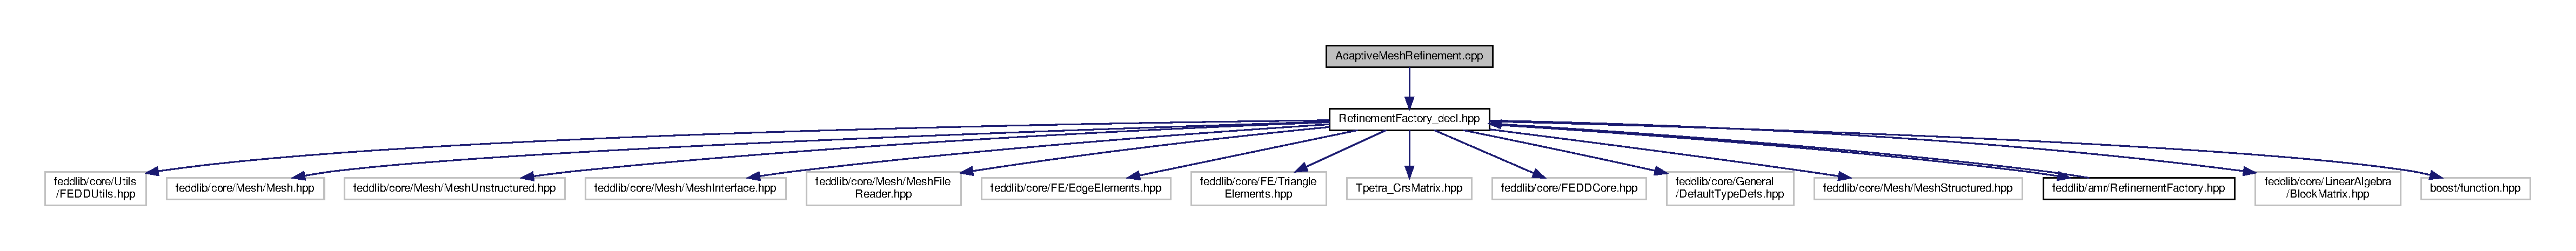
\includegraphics[width=350pt]{AdaptiveMeshRefinement_8cpp__incl}
\end{center}
\end{figure}

\hypertarget{AdaptiveMeshRefinement_8hpp}{}\section{Adaptive\+Mesh\+Refinement.\+hpp File Reference}
\label{AdaptiveMeshRefinement_8hpp}\index{Adaptive\+Mesh\+Refinement.\+hpp@{Adaptive\+Mesh\+Refinement.\+hpp}}
{\ttfamily \#include \char`\"{}Adaptive\+Mesh\+Refinement\+\_\+decl.\+hpp\char`\"{}}\newline
Include dependency graph for Adaptive\+Mesh\+Refinement.\+hpp\+:
\nopagebreak
\begin{figure}[H]
\begin{center}
\leavevmode
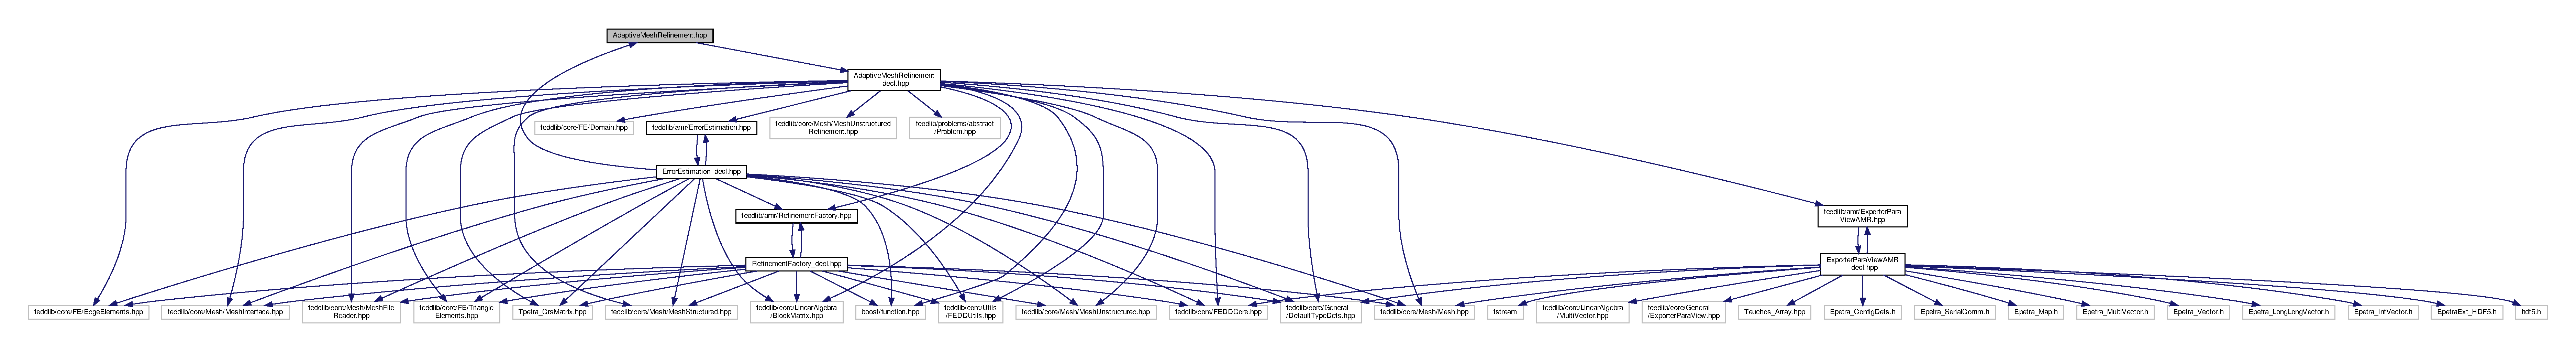
\includegraphics[width=350pt]{AdaptiveMeshRefinement_8hpp__incl}
\end{center}
\end{figure}
This graph shows which files directly or indirectly include this file\+:
\nopagebreak
\begin{figure}[H]
\begin{center}
\leavevmode
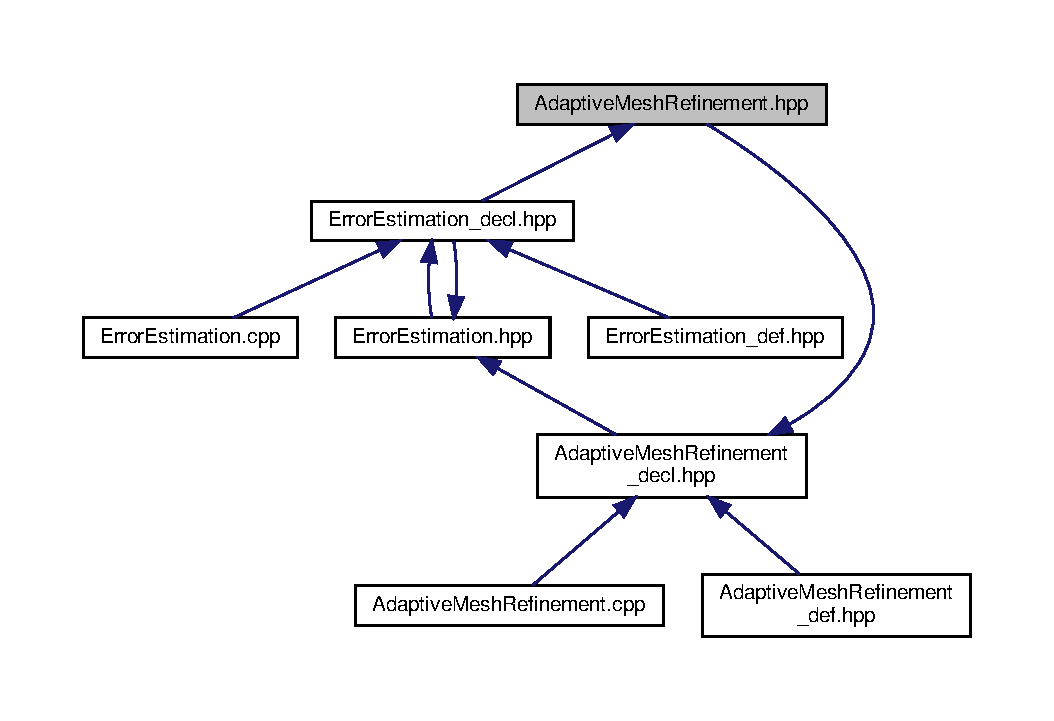
\includegraphics[width=350pt]{AdaptiveMeshRefinement_8hpp__dep__incl}
\end{center}
\end{figure}

\hypertarget{AdaptiveMeshRefinement__decl_8hpp}{}\section{Adaptive\+Mesh\+Refinement\+\_\+decl.\+hpp File Reference}
\label{AdaptiveMeshRefinement__decl_8hpp}\index{Adaptive\+Mesh\+Refinement\+\_\+decl.\+hpp@{Adaptive\+Mesh\+Refinement\+\_\+decl.\+hpp}}
{\ttfamily \#include \char`\"{}feddlib/core/\+Utils/\+F\+E\+D\+D\+Utils.\+hpp\char`\"{}}\newline
{\ttfamily \#include \char`\"{}feddlib/core/\+Mesh/\+Mesh.\+hpp\char`\"{}}\newline
{\ttfamily \#include \char`\"{}feddlib/core/\+Mesh/\+Mesh\+Unstructured.\+hpp\char`\"{}}\newline
{\ttfamily \#include \char`\"{}feddlib/core/\+Mesh/\+Mesh\+Interface.\+hpp\char`\"{}}\newline
{\ttfamily \#include \char`\"{}feddlib/core/\+Mesh/\+Mesh\+File\+Reader.\+hpp\char`\"{}}\newline
{\ttfamily \#include \char`\"{}feddlib/core/\+F\+E/\+Edge\+Elements.\+hpp\char`\"{}}\newline
{\ttfamily \#include \char`\"{}feddlib/core/\+F\+E/\+Triangle\+Elements.\+hpp\char`\"{}}\newline
{\ttfamily \#include \char`\"{}feddlib/core/\+F\+E/\+Domain.\+hpp\char`\"{}}\newline
{\ttfamily \#include $<$Tpetra\+\_\+\+Crs\+Matrix.\+hpp$>$}\newline
{\ttfamily \#include \char`\"{}feddlib/core/\+F\+E\+D\+D\+Core.\+hpp\char`\"{}}\newline
{\ttfamily \#include \char`\"{}feddlib/core/\+General/\+Default\+Type\+Defs.\+hpp\char`\"{}}\newline
{\ttfamily \#include \char`\"{}feddlib/core/\+Mesh/\+Mesh\+Structured.\+hpp\char`\"{}}\newline
{\ttfamily \#include \char`\"{}feddlib/core/\+Mesh/\+Mesh\+Unstructured\+Refinement.\+hpp\char`\"{}}\newline
{\ttfamily \#include \char`\"{}feddlib/core/\+Linear\+Algebra/\+Block\+Matrix.\+hpp\char`\"{}}\newline
{\ttfamily \#include $<$boost/function.\+hpp$>$}\newline
{\ttfamily \#include \char`\"{}feddlib/problems/abstract/\+Problem.\+hpp\char`\"{}}\newline
{\ttfamily \#include \char`\"{}feddlib/amr/\+Exporter\+Para\+View\+A\+M\+R.\+hpp\char`\"{}}\newline
{\ttfamily \#include \char`\"{}feddlib/amr/\+Error\+Estimation.\+hpp\char`\"{}}\newline
{\ttfamily \#include \char`\"{}feddlib/amr/\+Refinement\+Factory.\+hpp\char`\"{}}\newline
Include dependency graph for Adaptive\+Mesh\+Refinement\+\_\+decl.\+hpp\+:
\nopagebreak
\begin{figure}[H]
\begin{center}
\leavevmode
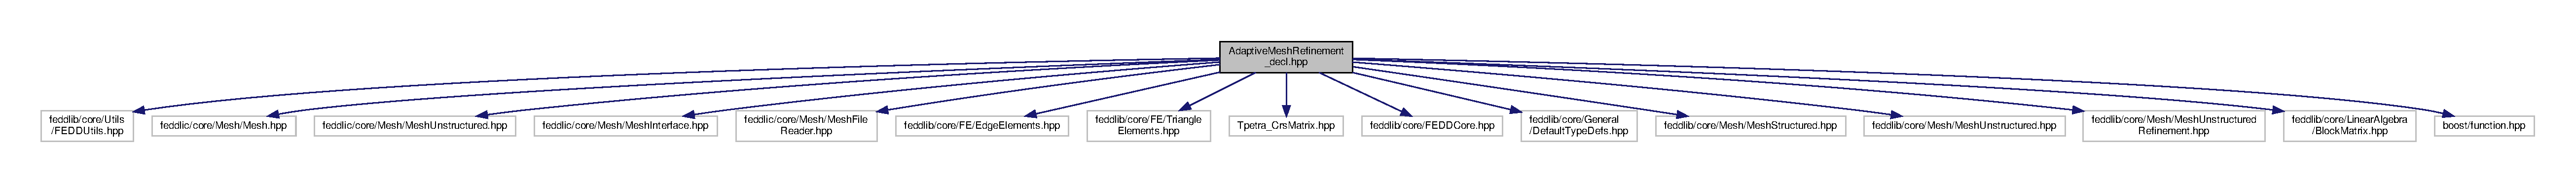
\includegraphics[width=350pt]{AdaptiveMeshRefinement__decl_8hpp__incl}
\end{center}
\end{figure}
This graph shows which files directly or indirectly include this file\+:
\nopagebreak
\begin{figure}[H]
\begin{center}
\leavevmode
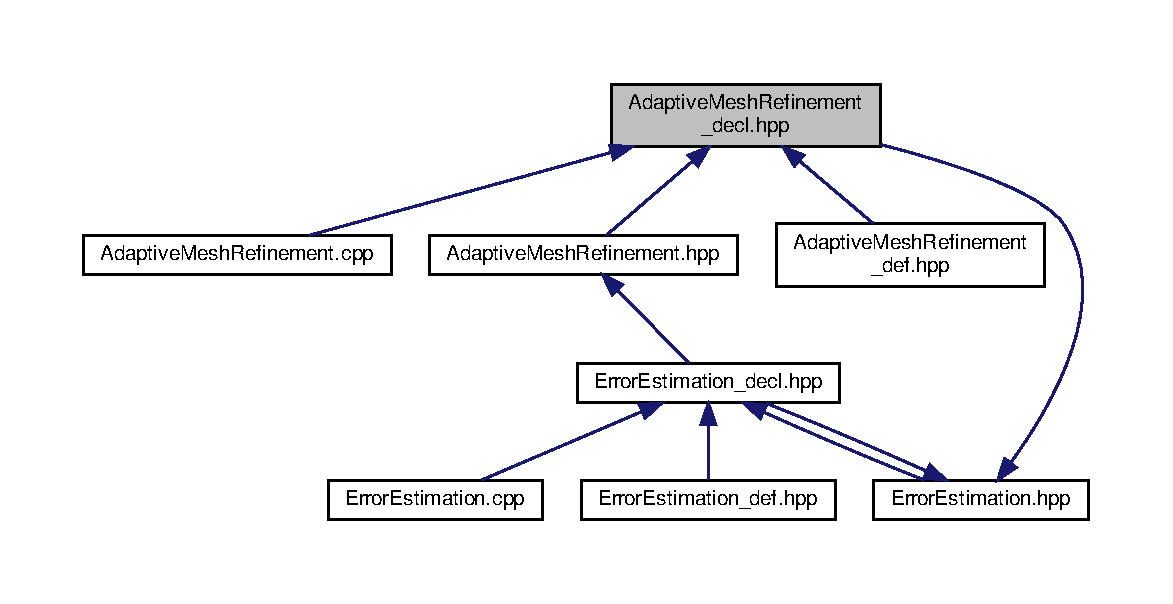
\includegraphics[width=350pt]{AdaptiveMeshRefinement__decl_8hpp__dep__incl}
\end{center}
\end{figure}
\subsection*{Data Structures}
\begin{DoxyCompactItemize}
\item 
class \hyperlink{classFEDD_1_1AdaptiveMeshRefinement}{F\+E\+D\+D\+::\+Adaptive\+Mesh\+Refinement$<$ S\+C, L\+O, G\+O, N\+O $>$}
\end{DoxyCompactItemize}
\subsection*{Namespaces}
\begin{DoxyCompactItemize}
\item 
 \hyperlink{namespaceFEDD}{F\+E\+DD}
\begin{DoxyCompactList}\small\item\em Mesh\+Unstructured\+Refinement. \end{DoxyCompactList}\end{DoxyCompactItemize}

\hypertarget{AdaptiveMeshRefinement__def_8hpp}{}\section{Adaptive\+Mesh\+Refinement\+\_\+def.\+hpp File Reference}
\label{AdaptiveMeshRefinement__def_8hpp}\index{Adaptive\+Mesh\+Refinement\+\_\+def.\+hpp@{Adaptive\+Mesh\+Refinement\+\_\+def.\+hpp}}
{\ttfamily \#include \char`\"{}Adaptive\+Mesh\+Refinement\+\_\+decl.\+hpp\char`\"{}}\newline
{\ttfamily \#include \char`\"{}feddlib/core/\+Linear\+Algebra/\+Multi\+Vector\+\_\+def.\+hpp\char`\"{}}\newline
{\ttfamily \#include $<$chrono$>$}\newline
Include dependency graph for Adaptive\+Mesh\+Refinement\+\_\+def.\+hpp\+:\nopagebreak
\begin{figure}[H]
\begin{center}
\leavevmode
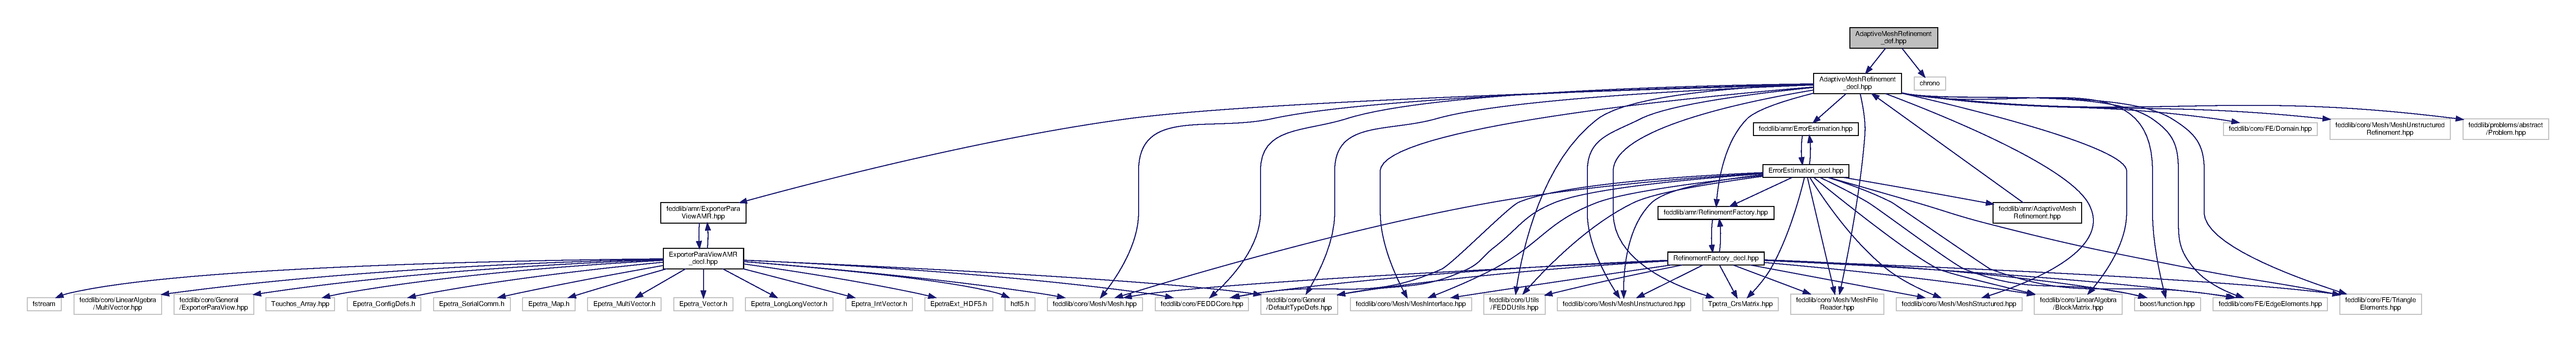
\includegraphics[width=350pt]{AdaptiveMeshRefinement__def_8hpp__incl}
\end{center}
\end{figure}
\subsection*{Namespaces}
\begin{DoxyCompactItemize}
\item 
 \hyperlink{namespaceFEDD}{F\+E\+DD}
\begin{DoxyCompactList}\small\item\em Mesh\+Unstructured\+Refinement. \end{DoxyCompactList}\end{DoxyCompactItemize}
\subsection*{Macros}
\begin{DoxyCompactItemize}
\item 
\#define \hyperlink{AdaptiveMeshRefinement__def_8hpp_aa1a5c1388eec07e84b71fa4f0f534bda}{M\+E\+S\+H\+\_\+\+T\+I\+M\+E\+R\+\_\+\+S\+T\+A\+RT}(A,  S)~Teuchos\+::\+R\+CP$<$Teuchos\+::\+Time\+Monitor$>$ A = Teuchos\+::rcp(new Teuchos\+::\+Time\+Monitor($\ast$Teuchos\+::\+Time\+Monitor\+::get\+New\+Timer(std\+::string(\char`\"{}Mesh Refinement\char`\"{}) + std\+::string(S))));
\item 
\#define \hyperlink{AdaptiveMeshRefinement__def_8hpp_a3c920e3d75aa84a024c9750ea98dd8a0}{M\+E\+S\+H\+\_\+\+T\+I\+M\+E\+R\+\_\+\+S\+T\+OP}(A)~A.\+reset();
\end{DoxyCompactItemize}


\subsection{Macro Definition Documentation}
\mbox{\Hypertarget{AdaptiveMeshRefinement__def_8hpp_aa1a5c1388eec07e84b71fa4f0f534bda}\label{AdaptiveMeshRefinement__def_8hpp_aa1a5c1388eec07e84b71fa4f0f534bda}} 
\index{Adaptive\+Mesh\+Refinement\+\_\+def.\+hpp@{Adaptive\+Mesh\+Refinement\+\_\+def.\+hpp}!M\+E\+S\+H\+\_\+\+T\+I\+M\+E\+R\+\_\+\+S\+T\+A\+RT@{M\+E\+S\+H\+\_\+\+T\+I\+M\+E\+R\+\_\+\+S\+T\+A\+RT}}
\index{M\+E\+S\+H\+\_\+\+T\+I\+M\+E\+R\+\_\+\+S\+T\+A\+RT@{M\+E\+S\+H\+\_\+\+T\+I\+M\+E\+R\+\_\+\+S\+T\+A\+RT}!Adaptive\+Mesh\+Refinement\+\_\+def.\+hpp@{Adaptive\+Mesh\+Refinement\+\_\+def.\+hpp}}
\subsubsection{\texorpdfstring{M\+E\+S\+H\+\_\+\+T\+I\+M\+E\+R\+\_\+\+S\+T\+A\+RT}{MESH\_TIMER\_START}}
{\footnotesize\ttfamily \#define M\+E\+S\+H\+\_\+\+T\+I\+M\+E\+R\+\_\+\+S\+T\+A\+RT(\begin{DoxyParamCaption}\item[{}]{A,  }\item[{}]{S }\end{DoxyParamCaption})~Teuchos\+::\+R\+CP$<$Teuchos\+::\+Time\+Monitor$>$ A = Teuchos\+::rcp(new Teuchos\+::\+Time\+Monitor($\ast$Teuchos\+::\+Time\+Monitor\+::get\+New\+Timer(std\+::string(\char`\"{}Mesh Refinement\char`\"{}) + std\+::string(S))));}

\mbox{\Hypertarget{AdaptiveMeshRefinement__def_8hpp_a3c920e3d75aa84a024c9750ea98dd8a0}\label{AdaptiveMeshRefinement__def_8hpp_a3c920e3d75aa84a024c9750ea98dd8a0}} 
\index{Adaptive\+Mesh\+Refinement\+\_\+def.\+hpp@{Adaptive\+Mesh\+Refinement\+\_\+def.\+hpp}!M\+E\+S\+H\+\_\+\+T\+I\+M\+E\+R\+\_\+\+S\+T\+OP@{M\+E\+S\+H\+\_\+\+T\+I\+M\+E\+R\+\_\+\+S\+T\+OP}}
\index{M\+E\+S\+H\+\_\+\+T\+I\+M\+E\+R\+\_\+\+S\+T\+OP@{M\+E\+S\+H\+\_\+\+T\+I\+M\+E\+R\+\_\+\+S\+T\+OP}!Adaptive\+Mesh\+Refinement\+\_\+def.\+hpp@{Adaptive\+Mesh\+Refinement\+\_\+def.\+hpp}}
\subsubsection{\texorpdfstring{M\+E\+S\+H\+\_\+\+T\+I\+M\+E\+R\+\_\+\+S\+T\+OP}{MESH\_TIMER\_STOP}}
{\footnotesize\ttfamily \#define M\+E\+S\+H\+\_\+\+T\+I\+M\+E\+R\+\_\+\+S\+T\+OP(\begin{DoxyParamCaption}\item[{}]{A }\end{DoxyParamCaption})~A.\+reset();}


\hypertarget{ErrorEstimation_8cpp}{}\section{Error\+Estimation.\+cpp File Reference}
\label{ErrorEstimation_8cpp}\index{Error\+Estimation.\+cpp@{Error\+Estimation.\+cpp}}
{\ttfamily \#include \char`\"{}Error\+Estimation\+\_\+decl.\+hpp\char`\"{}}\newline
Include dependency graph for Error\+Estimation.\+cpp\+:
\nopagebreak
\begin{figure}[H]
\begin{center}
\leavevmode
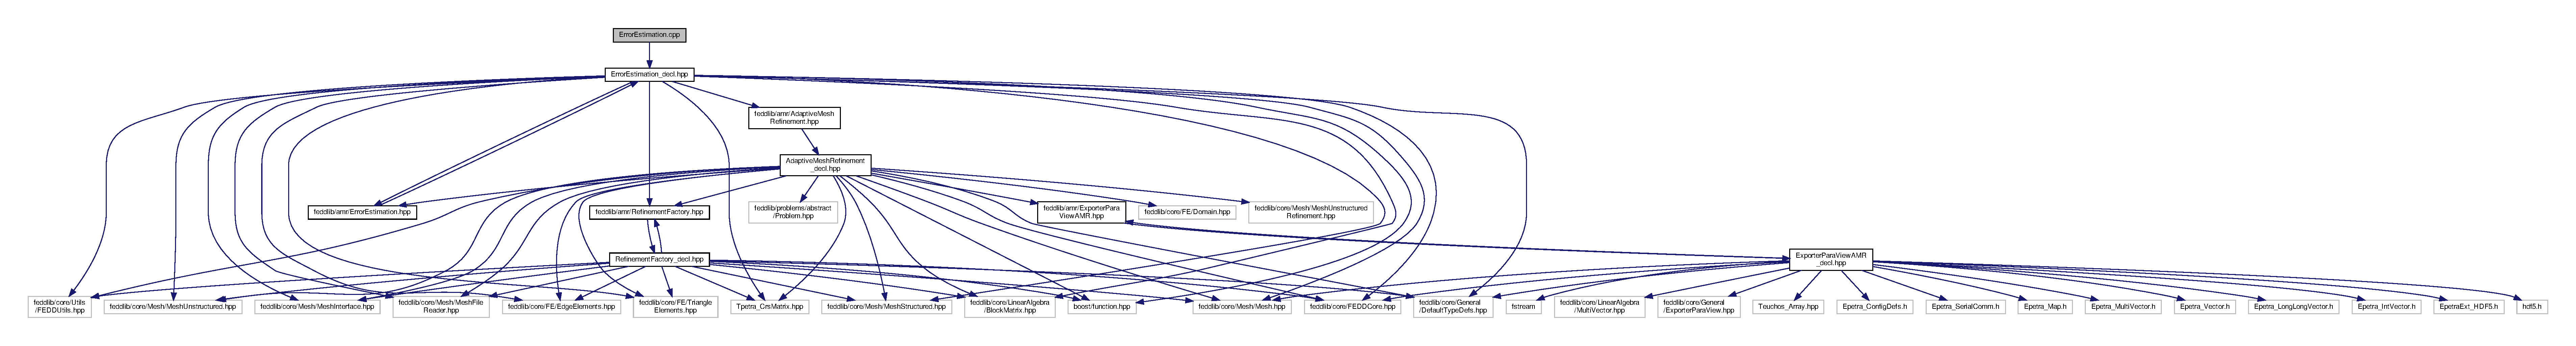
\includegraphics[width=350pt]{ErrorEstimation_8cpp__incl}
\end{center}
\end{figure}

\hypertarget{ErrorEstimation_8hpp}{}\section{Error\+Estimation.\+hpp File Reference}
\label{ErrorEstimation_8hpp}\index{Error\+Estimation.\+hpp@{Error\+Estimation.\+hpp}}
{\ttfamily \#include \char`\"{}Error\+Estimation\+\_\+decl.\+hpp\char`\"{}}\newline
Include dependency graph for Error\+Estimation.\+hpp\+:\nopagebreak
\begin{figure}[H]
\begin{center}
\leavevmode
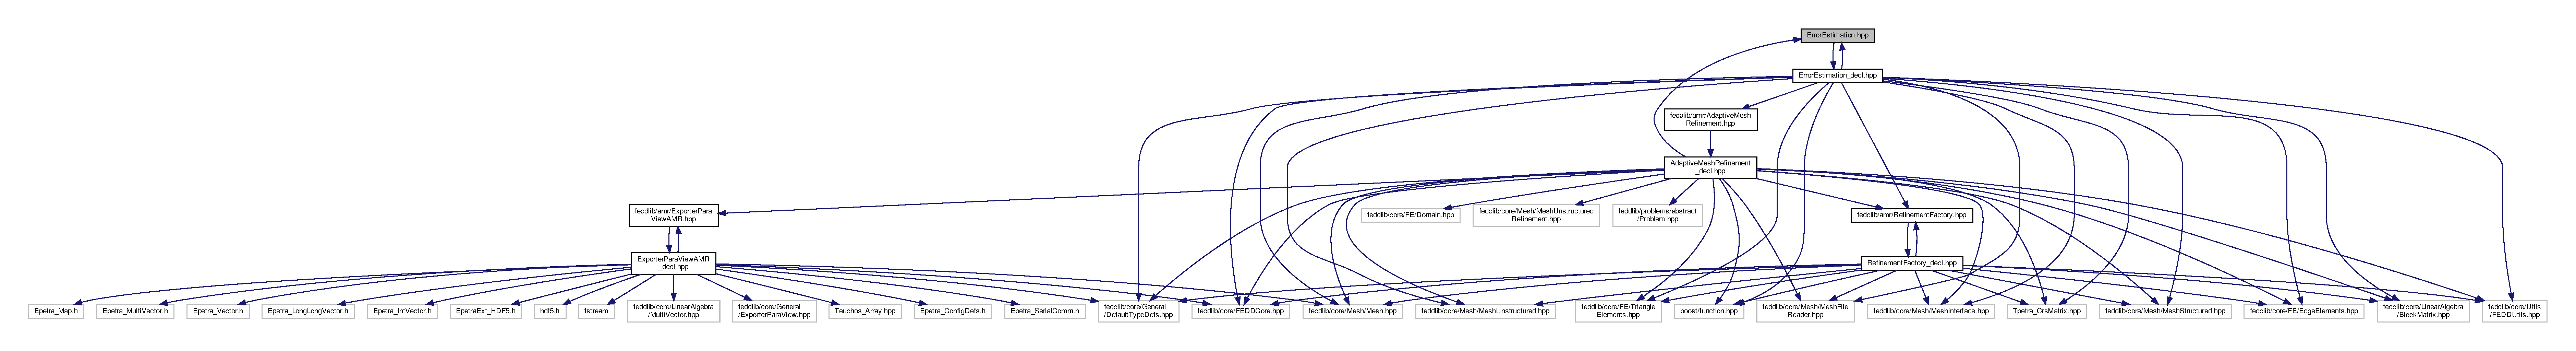
\includegraphics[width=350pt]{ErrorEstimation_8hpp__incl}
\end{center}
\end{figure}

\hypertarget{ErrorEstimation__decl_8hpp}{}\section{Error\+Estimation\+\_\+decl.\+hpp File Reference}
\label{ErrorEstimation__decl_8hpp}\index{Error\+Estimation\+\_\+decl.\+hpp@{Error\+Estimation\+\_\+decl.\+hpp}}
{\ttfamily \#include \char`\"{}feddlib/core/\+Utils/\+F\+E\+D\+D\+Utils.\+hpp\char`\"{}}\newline
{\ttfamily \#include \char`\"{}feddlic/core/\+Mesh/\+Mesh.\+hpp\char`\"{}}\newline
{\ttfamily \#include \char`\"{}feddlic/core/\+Mesh/\+Mesh\+Unstructured.\+hpp\char`\"{}}\newline
{\ttfamily \#include \char`\"{}feddlic/core/\+Mesh/\+Mesh\+Interface.\+hpp\char`\"{}}\newline
{\ttfamily \#include \char`\"{}feddlic/core/\+Mesh/\+Mesh\+File\+Reader.\+hpp\char`\"{}}\newline
{\ttfamily \#include \char`\"{}feddlib/core/\+F\+E/\+Edge\+Elements.\+hpp\char`\"{}}\newline
{\ttfamily \#include \char`\"{}feddlib/core/\+F\+E/\+Triangle\+Elements.\+hpp\char`\"{}}\newline
{\ttfamily \#include \char`\"{}feddlib/core/\+F\+E/\+Edge\+Elements\+New.\+hpp\char`\"{}}\newline
{\ttfamily \#include $<$Tpetra\+\_\+\+Crs\+Matrix.\+hpp$>$}\newline
{\ttfamily \#include \char`\"{}feddlib/core/\+F\+E\+D\+D\+Core.\+hpp\char`\"{}}\newline
{\ttfamily \#include \char`\"{}feddlib/core/\+General/\+Default\+Type\+Defs.\+hpp\char`\"{}}\newline
{\ttfamily \#include \char`\"{}feddlib/core/\+Mesh/\+Mesh\+Structured.\+hpp\char`\"{}}\newline
{\ttfamily \#include \char`\"{}feddlib/core/\+Mesh/\+Mesh\+Unstructured.\+hpp\char`\"{}}\newline
{\ttfamily \#include \char`\"{}feddlib/core/\+Mesh/\+Error\+Estimation.\+hpp\char`\"{}}\newline
{\ttfamily \#include \char`\"{}feddlib/core/\+Linear\+Algebra/\+Block\+Matrix.\+hpp\char`\"{}}\newline
{\ttfamily \#include $<$boost/function.\+hpp$>$}\newline
Include dependency graph for Error\+Estimation\+\_\+decl.\+hpp\+:\nopagebreak
\begin{figure}[H]
\begin{center}
\leavevmode
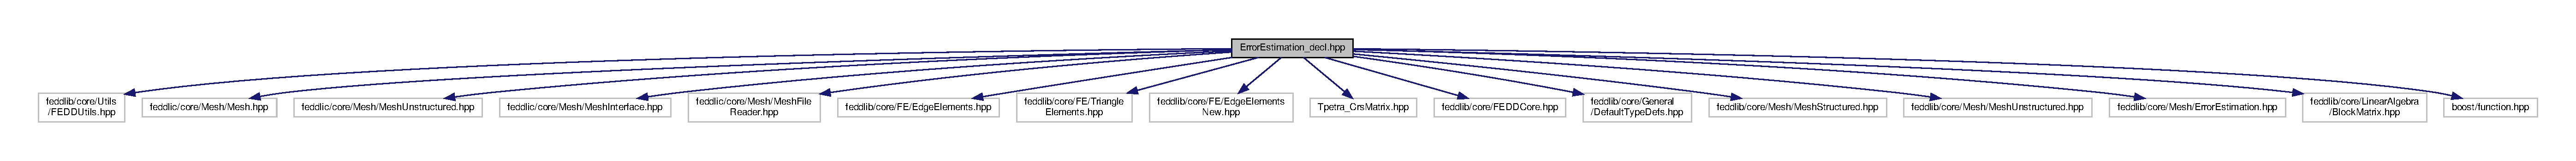
\includegraphics[width=350pt]{ErrorEstimation__decl_8hpp__incl}
\end{center}
\end{figure}
This graph shows which files directly or indirectly include this file\+:\nopagebreak
\begin{figure}[H]
\begin{center}
\leavevmode
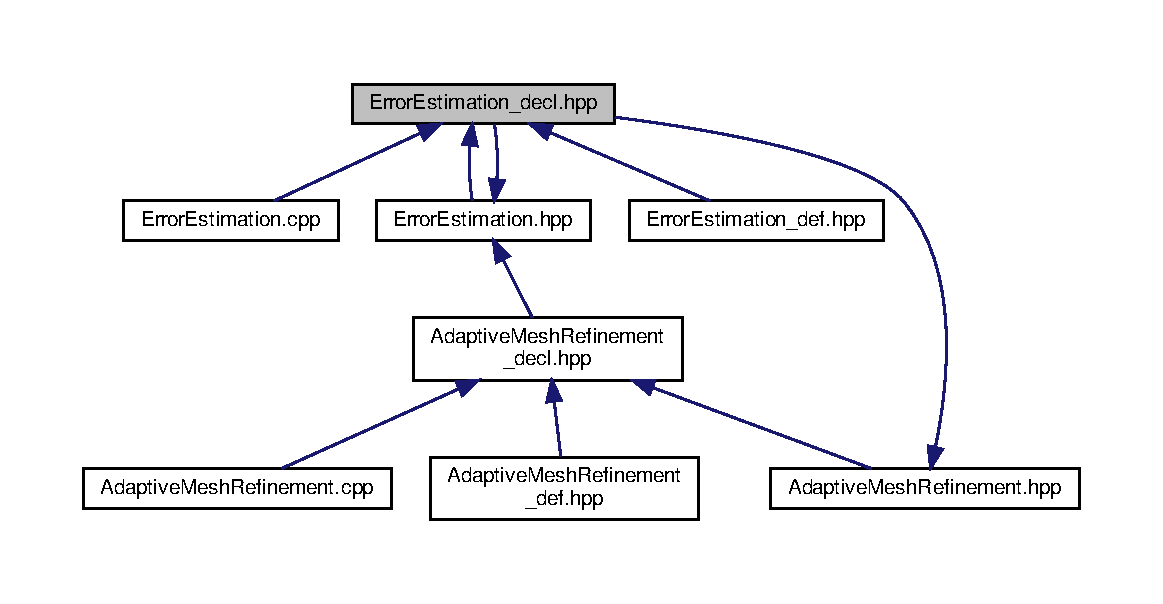
\includegraphics[width=350pt]{ErrorEstimation__decl_8hpp__dep__incl}
\end{center}
\end{figure}
\subsection*{Data Structures}
\begin{DoxyCompactItemize}
\item 
class \hyperlink{classFEDD_1_1ErrorEstimation}{F\+E\+D\+D\+::\+Error\+Estimation$<$ S\+C, L\+O, G\+O, N\+O $>$}
\end{DoxyCompactItemize}
\subsection*{Namespaces}
\begin{DoxyCompactItemize}
\item 
 \hyperlink{namespaceFEDD}{F\+E\+DD}
\begin{DoxyCompactList}\small\item\em Mesh\+Unstructured\+Refinement. \end{DoxyCompactList}\end{DoxyCompactItemize}

\hypertarget{ErrorEstimation__def_8hpp}{}\section{Error\+Estimation\+\_\+def.\+hpp File Reference}
\label{ErrorEstimation__def_8hpp}\index{Error\+Estimation\+\_\+def.\+hpp@{Error\+Estimation\+\_\+def.\+hpp}}
{\ttfamily \#include \char`\"{}Error\+Estimation\+\_\+decl.\+hpp\char`\"{}}\newline
{\ttfamily \#include \char`\"{}feddlib/core/\+Linear\+Algebra/\+Multi\+Vector\+\_\+def.\+hpp\char`\"{}}\newline
{\ttfamily \#include $<$chrono$>$}\newline
Include dependency graph for Error\+Estimation\+\_\+def.\+hpp\+:\nopagebreak
\begin{figure}[H]
\begin{center}
\leavevmode
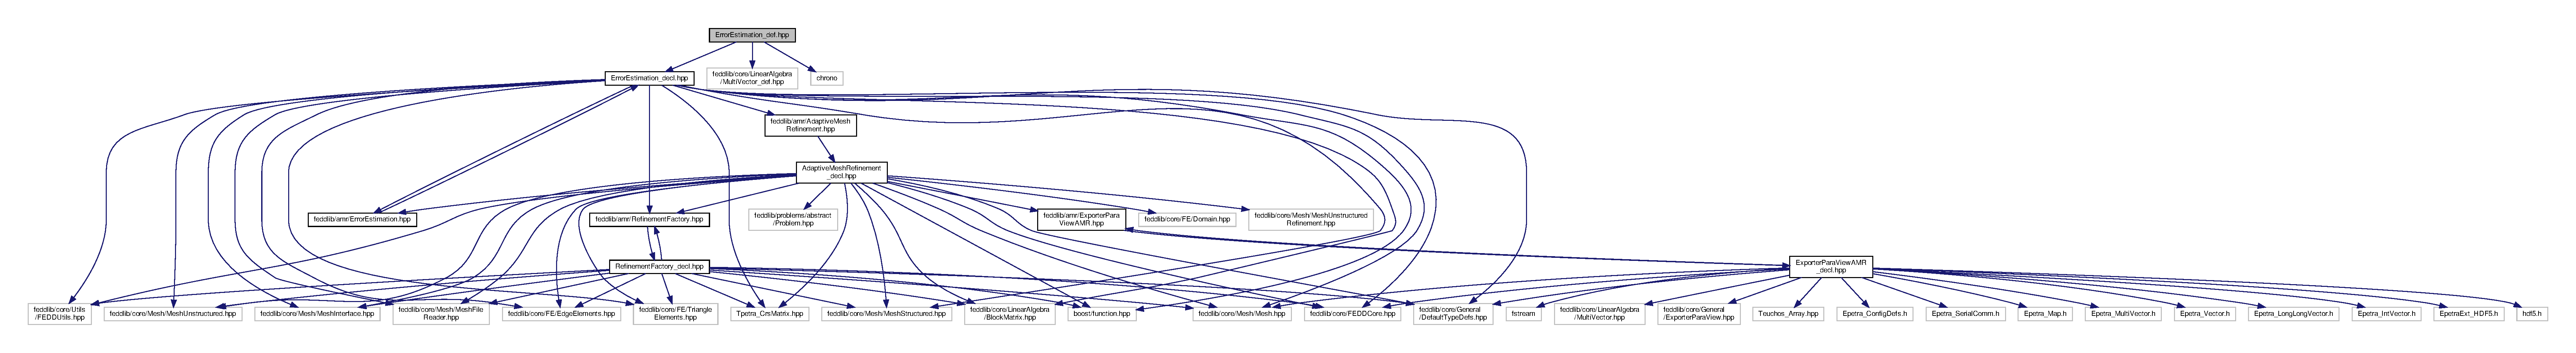
\includegraphics[width=350pt]{ErrorEstimation__def_8hpp__incl}
\end{center}
\end{figure}
\subsection*{Namespaces}
\begin{DoxyCompactItemize}
\item 
 \hyperlink{namespaceFEDD}{F\+E\+DD}
\begin{DoxyCompactList}\small\item\em Mesh\+Unstructured\+Refinement. \end{DoxyCompactList}\end{DoxyCompactItemize}
\subsection*{Macros}
\begin{DoxyCompactItemize}
\item 
\#define \hyperlink{ErrorEstimation__def_8hpp_aa1a5c1388eec07e84b71fa4f0f534bda}{M\+E\+S\+H\+\_\+\+T\+I\+M\+E\+R\+\_\+\+S\+T\+A\+RT}(A,  S)~Teuchos\+::\+R\+CP$<$Teuchos\+::\+Time\+Monitor$>$ A = Teuchos\+::rcp(new Teuchos\+::\+Time\+Monitor($\ast$Teuchos\+::\+Time\+Monitor\+::get\+New\+Timer(std\+::string(\char`\"{}Mesh Refinement\char`\"{}) + std\+::string(S))));
\item 
\#define \hyperlink{ErrorEstimation__def_8hpp_a3c920e3d75aa84a024c9750ea98dd8a0}{M\+E\+S\+H\+\_\+\+T\+I\+M\+E\+R\+\_\+\+S\+T\+OP}(A)~A.\+reset();
\end{DoxyCompactItemize}


\subsection{Macro Definition Documentation}
\mbox{\Hypertarget{ErrorEstimation__def_8hpp_aa1a5c1388eec07e84b71fa4f0f534bda}\label{ErrorEstimation__def_8hpp_aa1a5c1388eec07e84b71fa4f0f534bda}} 
\index{Error\+Estimation\+\_\+def.\+hpp@{Error\+Estimation\+\_\+def.\+hpp}!M\+E\+S\+H\+\_\+\+T\+I\+M\+E\+R\+\_\+\+S\+T\+A\+RT@{M\+E\+S\+H\+\_\+\+T\+I\+M\+E\+R\+\_\+\+S\+T\+A\+RT}}
\index{M\+E\+S\+H\+\_\+\+T\+I\+M\+E\+R\+\_\+\+S\+T\+A\+RT@{M\+E\+S\+H\+\_\+\+T\+I\+M\+E\+R\+\_\+\+S\+T\+A\+RT}!Error\+Estimation\+\_\+def.\+hpp@{Error\+Estimation\+\_\+def.\+hpp}}
\subsubsection{\texorpdfstring{M\+E\+S\+H\+\_\+\+T\+I\+M\+E\+R\+\_\+\+S\+T\+A\+RT}{MESH\_TIMER\_START}}
{\footnotesize\ttfamily \#define M\+E\+S\+H\+\_\+\+T\+I\+M\+E\+R\+\_\+\+S\+T\+A\+RT(\begin{DoxyParamCaption}\item[{}]{A,  }\item[{}]{S }\end{DoxyParamCaption})~Teuchos\+::\+R\+CP$<$Teuchos\+::\+Time\+Monitor$>$ A = Teuchos\+::rcp(new Teuchos\+::\+Time\+Monitor($\ast$Teuchos\+::\+Time\+Monitor\+::get\+New\+Timer(std\+::string(\char`\"{}Mesh Refinement\char`\"{}) + std\+::string(S))));}

\mbox{\Hypertarget{ErrorEstimation__def_8hpp_a3c920e3d75aa84a024c9750ea98dd8a0}\label{ErrorEstimation__def_8hpp_a3c920e3d75aa84a024c9750ea98dd8a0}} 
\index{Error\+Estimation\+\_\+def.\+hpp@{Error\+Estimation\+\_\+def.\+hpp}!M\+E\+S\+H\+\_\+\+T\+I\+M\+E\+R\+\_\+\+S\+T\+OP@{M\+E\+S\+H\+\_\+\+T\+I\+M\+E\+R\+\_\+\+S\+T\+OP}}
\index{M\+E\+S\+H\+\_\+\+T\+I\+M\+E\+R\+\_\+\+S\+T\+OP@{M\+E\+S\+H\+\_\+\+T\+I\+M\+E\+R\+\_\+\+S\+T\+OP}!Error\+Estimation\+\_\+def.\+hpp@{Error\+Estimation\+\_\+def.\+hpp}}
\subsubsection{\texorpdfstring{M\+E\+S\+H\+\_\+\+T\+I\+M\+E\+R\+\_\+\+S\+T\+OP}{MESH\_TIMER\_STOP}}
{\footnotesize\ttfamily \#define M\+E\+S\+H\+\_\+\+T\+I\+M\+E\+R\+\_\+\+S\+T\+OP(\begin{DoxyParamCaption}\item[{}]{A }\end{DoxyParamCaption})~A.\+reset();}


\hypertarget{ExporterParaViewAMR_8cpp}{}\section{Exporter\+Para\+View\+A\+M\+R.\+cpp File Reference}
\label{ExporterParaViewAMR_8cpp}\index{Exporter\+Para\+View\+A\+M\+R.\+cpp@{Exporter\+Para\+View\+A\+M\+R.\+cpp}}
{\ttfamily \#include \char`\"{}Exporter\+Para\+View\+A\+M\+R\+\_\+decl.\+hpp\char`\"{}}\newline
Include dependency graph for Exporter\+Para\+View\+A\+M\+R.\+cpp\+:
\nopagebreak
\begin{figure}[H]
\begin{center}
\leavevmode
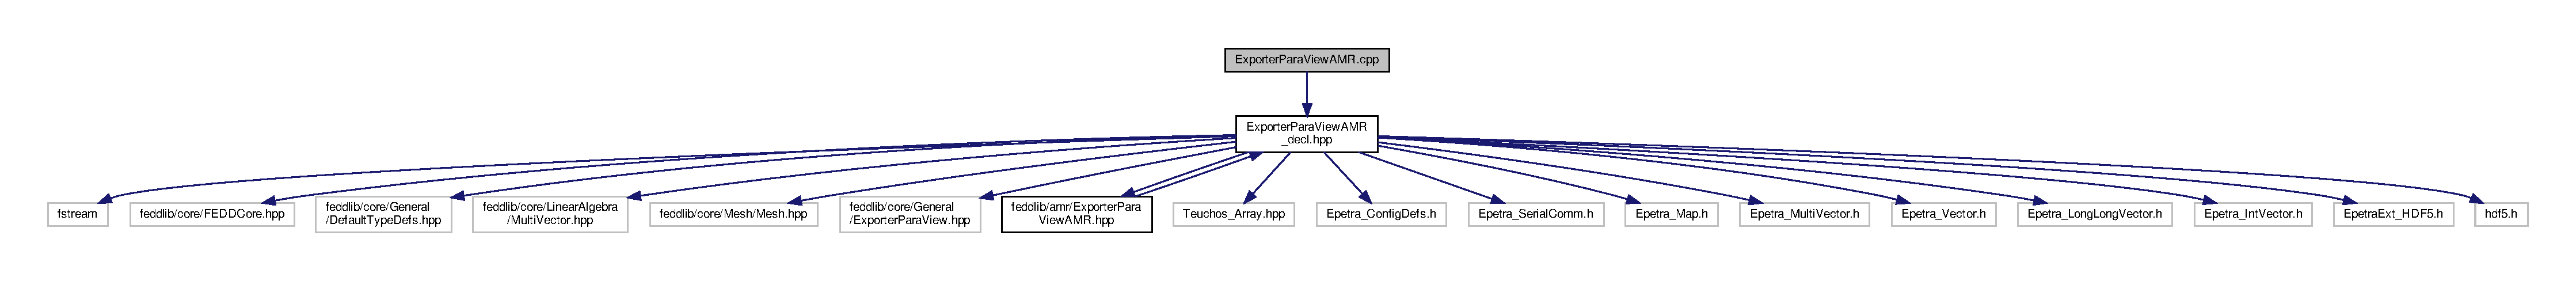
\includegraphics[width=350pt]{ExporterParaViewAMR_8cpp__incl}
\end{center}
\end{figure}

\hypertarget{ExporterParaViewAMR_8hpp}{}\section{Exporter\+Para\+View\+A\+M\+R.\+hpp File Reference}
\label{ExporterParaViewAMR_8hpp}\index{Exporter\+Para\+View\+A\+M\+R.\+hpp@{Exporter\+Para\+View\+A\+M\+R.\+hpp}}
{\ttfamily \#include \char`\"{}Exporter\+Para\+View\+A\+M\+R\+\_\+decl.\+hpp\char`\"{}}\newline
Include dependency graph for Exporter\+Para\+View\+A\+M\+R.\+hpp\+:
\nopagebreak
\begin{figure}[H]
\begin{center}
\leavevmode
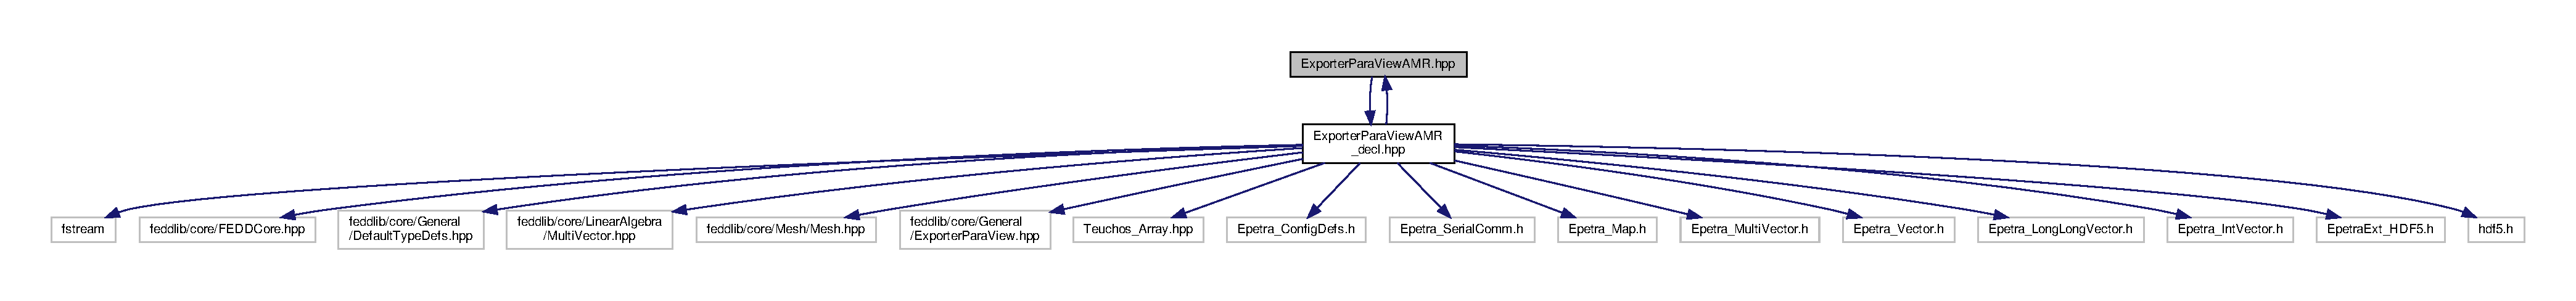
\includegraphics[width=350pt]{ExporterParaViewAMR_8hpp__incl}
\end{center}
\end{figure}
This graph shows which files directly or indirectly include this file\+:
\nopagebreak
\begin{figure}[H]
\begin{center}
\leavevmode
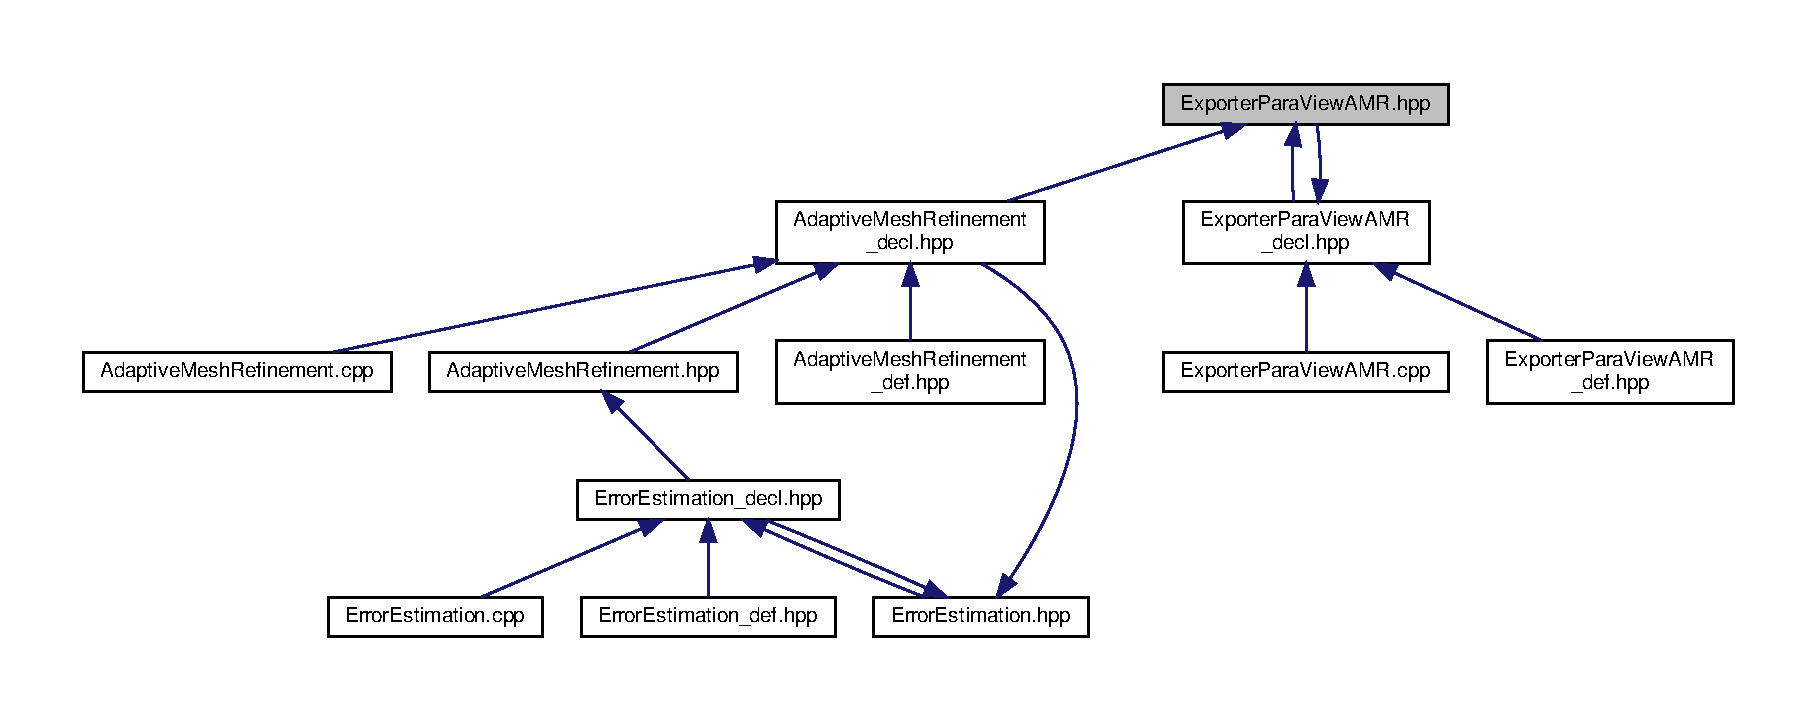
\includegraphics[width=350pt]{ExporterParaViewAMR_8hpp__dep__incl}
\end{center}
\end{figure}

\hypertarget{ExporterParaViewAMR__decl_8hpp}{}\section{Exporter\+Para\+View\+A\+M\+R\+\_\+decl.\+hpp File Reference}
\label{ExporterParaViewAMR__decl_8hpp}\index{Exporter\+Para\+View\+A\+M\+R\+\_\+decl.\+hpp@{Exporter\+Para\+View\+A\+M\+R\+\_\+decl.\+hpp}}
{\ttfamily \#include $<$fstream$>$}\newline
{\ttfamily \#include \char`\"{}feddlib/core/\+F\+E\+D\+D\+Core.\+hpp\char`\"{}}\newline
{\ttfamily \#include \char`\"{}feddlib/core/\+General/\+Default\+Type\+Defs.\+hpp\char`\"{}}\newline
{\ttfamily \#include \char`\"{}feddlib/core/\+Linear\+Algebra/\+Multi\+Vector.\+hpp\char`\"{}}\newline
{\ttfamily \#include \char`\"{}feddlib/core/\+Mesh/\+Mesh.\+hpp\char`\"{}}\newline
{\ttfamily \#include \char`\"{}feddlib/core/\+General/\+Exporter\+Para\+View.\+hpp\char`\"{}}\newline
{\ttfamily \#include \char`\"{}feddlib/amr/\+Exporter\+Para\+View\+A\+M\+R.\+hpp\char`\"{}}\newline
{\ttfamily \#include $<$Teuchos\+\_\+\+Array.\+hpp$>$}\newline
{\ttfamily \#include \char`\"{}Epetra\+\_\+\+Config\+Defs.\+h\char`\"{}}\newline
{\ttfamily \#include \char`\"{}Epetra\+\_\+\+Serial\+Comm.\+h\char`\"{}}\newline
{\ttfamily \#include $<$Epetra\+\_\+\+Map.\+h$>$}\newline
{\ttfamily \#include $<$Epetra\+\_\+\+Multi\+Vector.\+h$>$}\newline
{\ttfamily \#include $<$Epetra\+\_\+\+Vector.\+h$>$}\newline
{\ttfamily \#include $<$Epetra\+\_\+\+Long\+Long\+Vector.\+h$>$}\newline
{\ttfamily \#include $<$Epetra\+\_\+\+Int\+Vector.\+h$>$}\newline
{\ttfamily \#include $<$Epetra\+Ext\+\_\+\+H\+D\+F5.\+h$>$}\newline
{\ttfamily \#include $<$hdf5.\+h$>$}\newline
Include dependency graph for Exporter\+Para\+View\+A\+M\+R\+\_\+decl.\+hpp\+:
\nopagebreak
\begin{figure}[H]
\begin{center}
\leavevmode
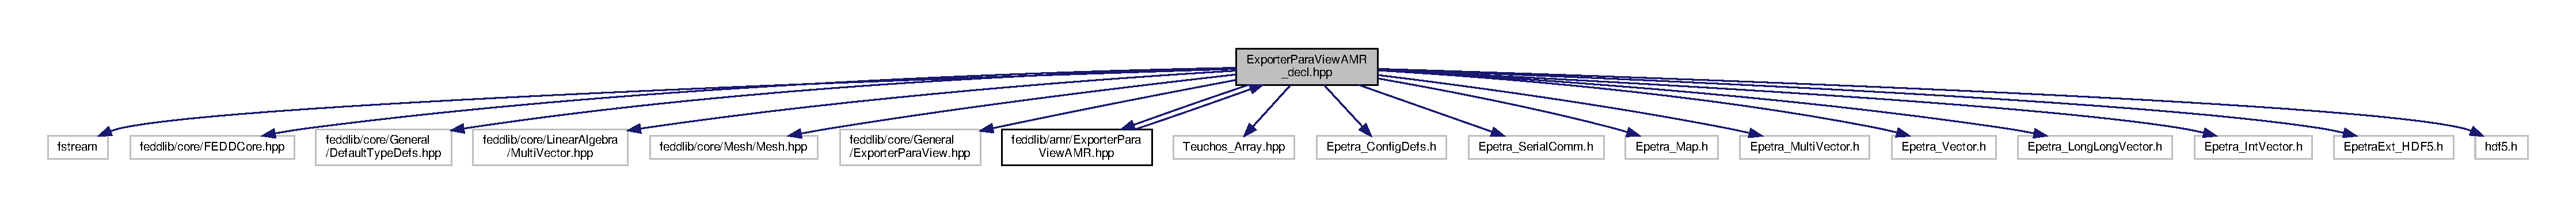
\includegraphics[width=350pt]{ExporterParaViewAMR__decl_8hpp__incl}
\end{center}
\end{figure}
This graph shows which files directly or indirectly include this file\+:
\nopagebreak
\begin{figure}[H]
\begin{center}
\leavevmode
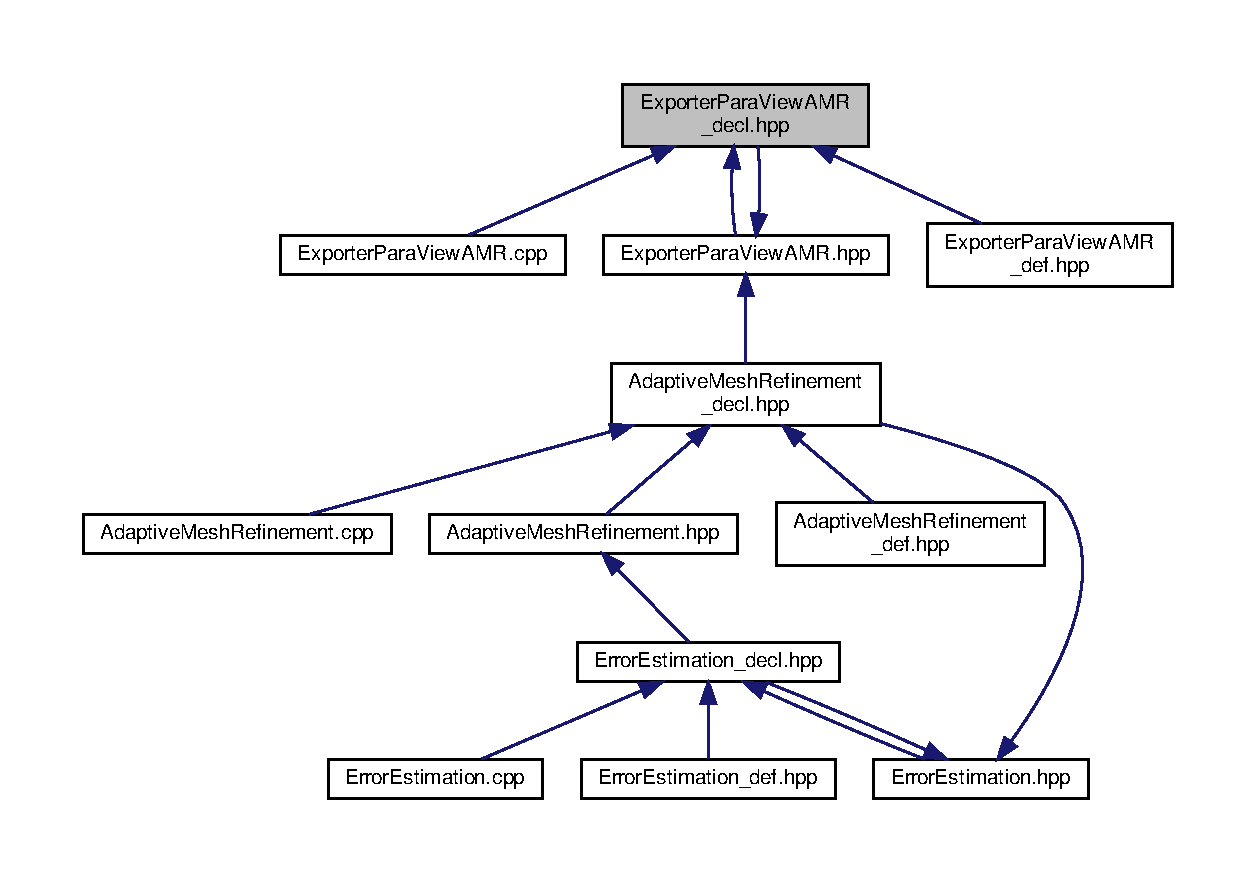
\includegraphics[width=350pt]{ExporterParaViewAMR__decl_8hpp__dep__incl}
\end{center}
\end{figure}
\subsection*{Data Structures}
\begin{DoxyCompactItemize}
\item 
class \hyperlink{classFEDD_1_1ExporterParaViewAMR}{F\+E\+D\+D\+::\+Exporter\+Para\+View\+A\+M\+R$<$ S\+C, L\+O, G\+O, N\+O $>$}
\end{DoxyCompactItemize}
\subsection*{Namespaces}
\begin{DoxyCompactItemize}
\item 
 \hyperlink{namespaceFEDD}{F\+E\+DD}
\begin{DoxyCompactList}\small\item\em Mesh\+Unstructured\+Refinement. \end{DoxyCompactList}\end{DoxyCompactItemize}

\hypertarget{ExporterParaViewAMR__def_8hpp}{}\section{Exporter\+Para\+View\+A\+M\+R\+\_\+def.\+hpp File Reference}
\label{ExporterParaViewAMR__def_8hpp}\index{Exporter\+Para\+View\+A\+M\+R\+\_\+def.\+hpp@{Exporter\+Para\+View\+A\+M\+R\+\_\+def.\+hpp}}
{\ttfamily \#include \char`\"{}Exporter\+Para\+View\+A\+M\+R\+\_\+decl.\+hpp\char`\"{}}\newline
Include dependency graph for Exporter\+Para\+View\+A\+M\+R\+\_\+def.\+hpp\+:
\nopagebreak
\begin{figure}[H]
\begin{center}
\leavevmode
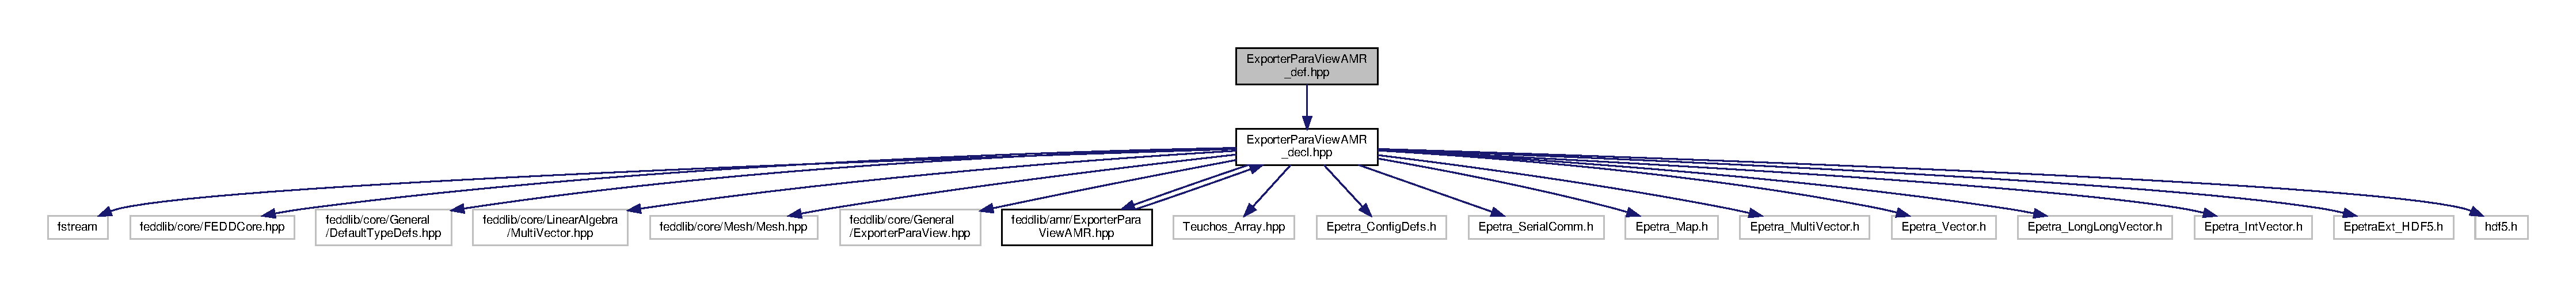
\includegraphics[width=350pt]{ExporterParaViewAMR__def_8hpp__incl}
\end{center}
\end{figure}
\subsection*{Namespaces}
\begin{DoxyCompactItemize}
\item 
 \hyperlink{namespaceFEDD}{F\+E\+DD}
\begin{DoxyCompactList}\small\item\em Mesh\+Unstructured\+Refinement. \end{DoxyCompactList}\end{DoxyCompactItemize}

\hypertarget{RefinementFactory_8cpp}{}\section{Refinement\+Factory.\+cpp File Reference}
\label{RefinementFactory_8cpp}\index{Refinement\+Factory.\+cpp@{Refinement\+Factory.\+cpp}}
{\ttfamily \#include \char`\"{}Refinement\+Factory\+\_\+decl.\+hpp\char`\"{}}\newline
Include dependency graph for Refinement\+Factory.\+cpp\+:\nopagebreak
\begin{figure}[H]
\begin{center}
\leavevmode
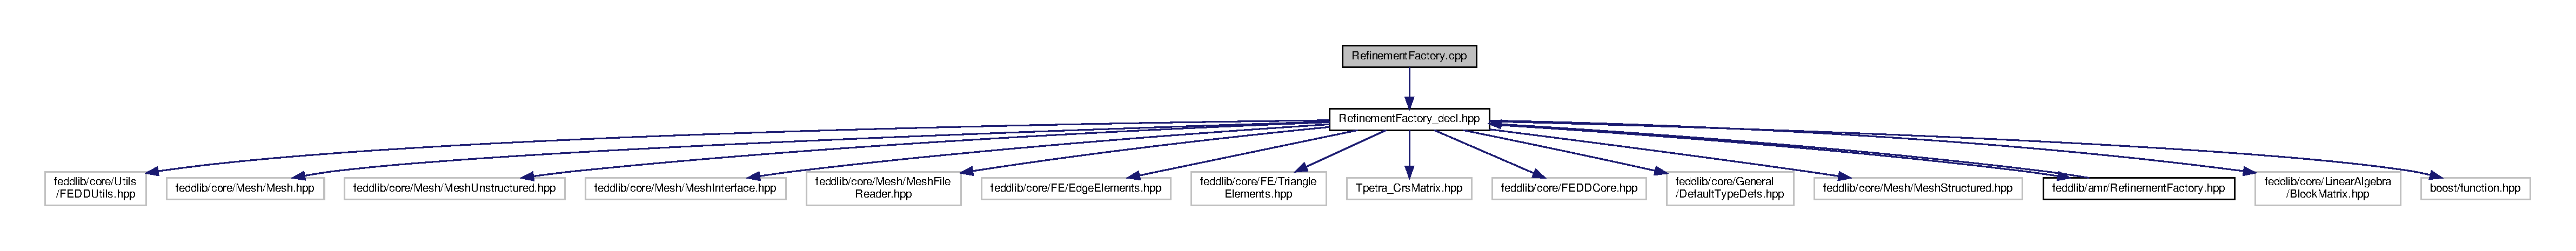
\includegraphics[width=350pt]{RefinementFactory_8cpp__incl}
\end{center}
\end{figure}

\hypertarget{RefinementFactory_8hpp}{}\section{Refinement\+Factory.\+hpp File Reference}
\label{RefinementFactory_8hpp}\index{Refinement\+Factory.\+hpp@{Refinement\+Factory.\+hpp}}
{\ttfamily \#include \char`\"{}Refinement\+Factory\+\_\+decl.\+hpp\char`\"{}}\newline
Include dependency graph for Refinement\+Factory.\+hpp\+:\nopagebreak
\begin{figure}[H]
\begin{center}
\leavevmode
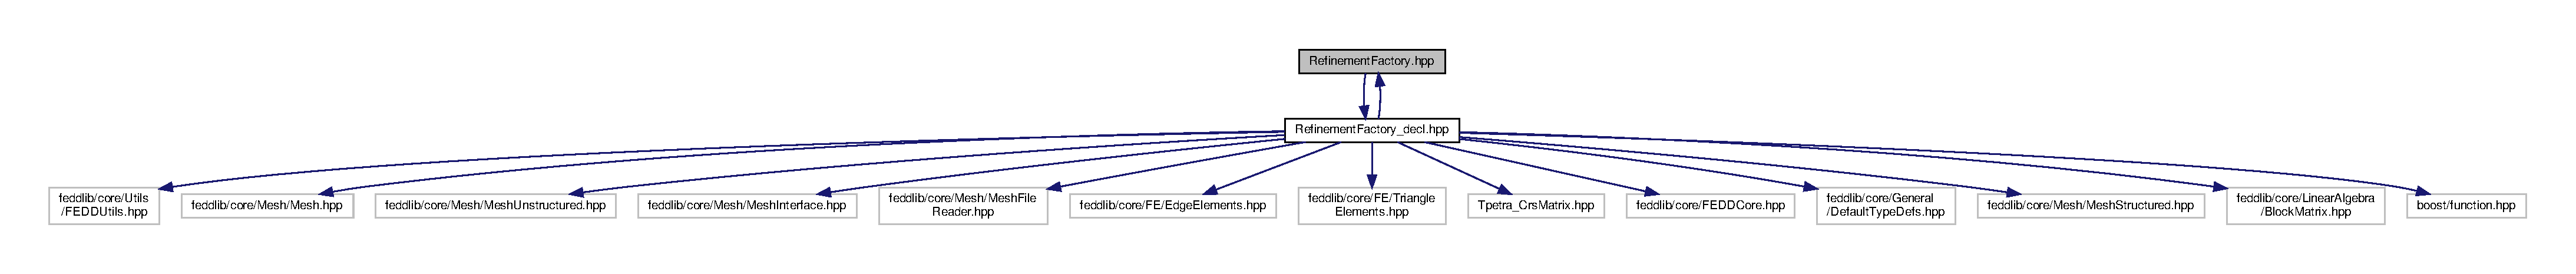
\includegraphics[width=350pt]{RefinementFactory_8hpp__incl}
\end{center}
\end{figure}
This graph shows which files directly or indirectly include this file\+:\nopagebreak
\begin{figure}[H]
\begin{center}
\leavevmode
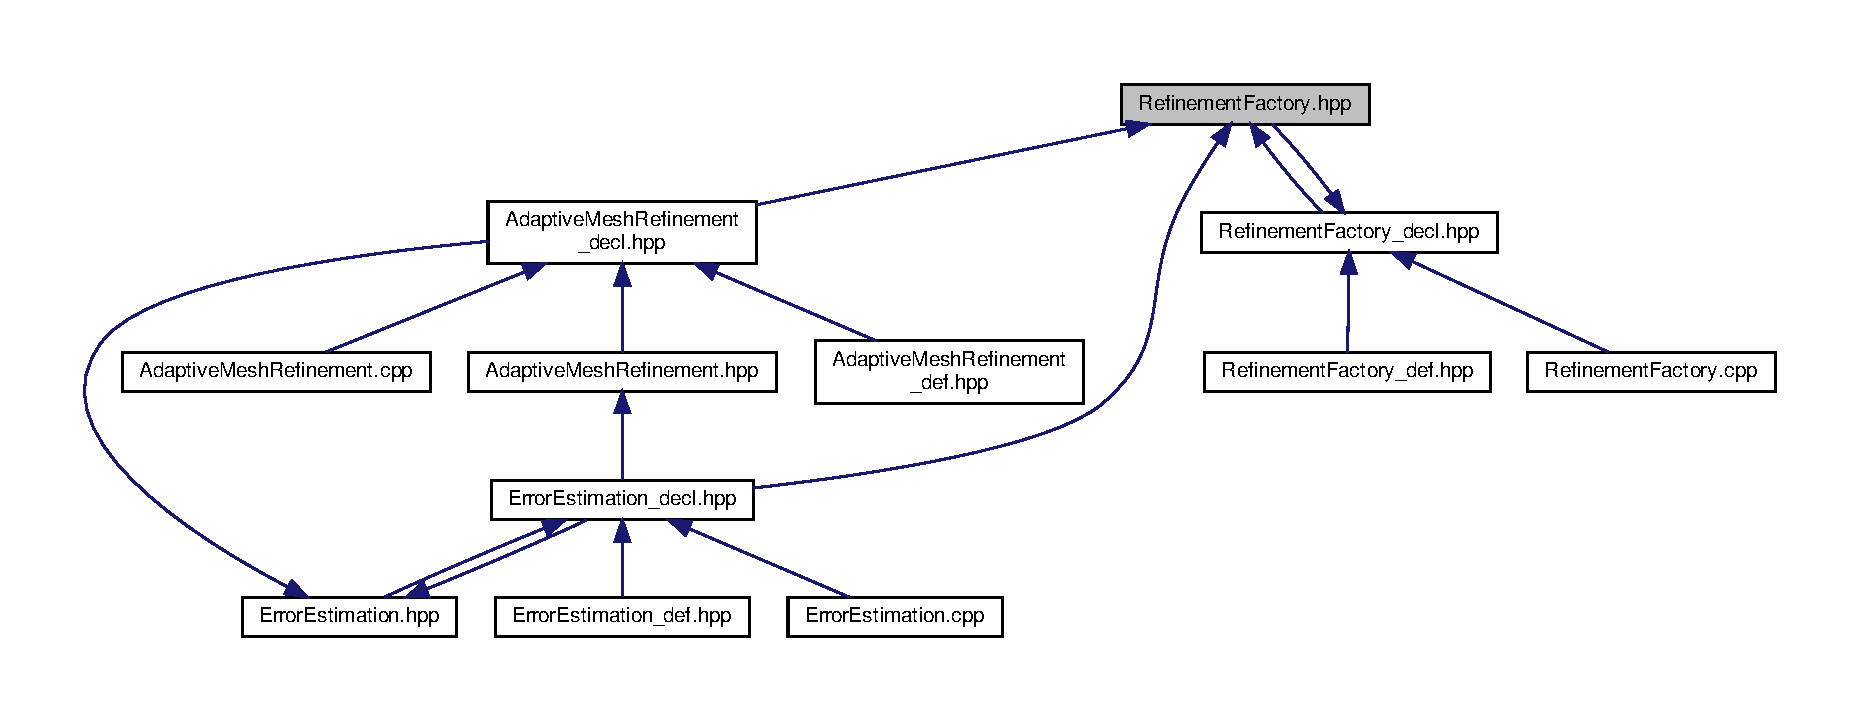
\includegraphics[width=350pt]{RefinementFactory_8hpp__dep__incl}
\end{center}
\end{figure}

\hypertarget{RefinementFactory__decl_8hpp}{}\section{Refinement\+Factory\+\_\+decl.\+hpp File Reference}
\label{RefinementFactory__decl_8hpp}\index{Refinement\+Factory\+\_\+decl.\+hpp@{Refinement\+Factory\+\_\+decl.\+hpp}}
{\ttfamily \#include \char`\"{}feddlib/core/\+Utils/\+F\+E\+D\+D\+Utils.\+hpp\char`\"{}}\newline
{\ttfamily \#include \char`\"{}feddlib/core/\+Mesh/\+Mesh.\+hpp\char`\"{}}\newline
{\ttfamily \#include \char`\"{}feddlib/core/\+Mesh/\+Mesh\+Unstructured.\+hpp\char`\"{}}\newline
{\ttfamily \#include \char`\"{}feddlib/core/\+Mesh/\+Mesh\+Interface.\+hpp\char`\"{}}\newline
{\ttfamily \#include \char`\"{}feddlib/core/\+Mesh/\+Mesh\+File\+Reader.\+hpp\char`\"{}}\newline
{\ttfamily \#include \char`\"{}feddlib/core/\+F\+E/\+Edge\+Elements.\+hpp\char`\"{}}\newline
{\ttfamily \#include \char`\"{}feddlib/core/\+F\+E/\+Triangle\+Elements.\+hpp\char`\"{}}\newline
{\ttfamily \#include $<$Tpetra\+\_\+\+Crs\+Matrix.\+hpp$>$}\newline
{\ttfamily \#include \char`\"{}feddlib/core/\+F\+E\+D\+D\+Core.\+hpp\char`\"{}}\newline
{\ttfamily \#include \char`\"{}feddlib/core/\+General/\+Default\+Type\+Defs.\+hpp\char`\"{}}\newline
{\ttfamily \#include \char`\"{}feddlib/core/\+Mesh/\+Mesh\+Structured.\+hpp\char`\"{}}\newline
{\ttfamily \#include \char`\"{}feddlib/amr/\+Refinement\+Factory.\+hpp\char`\"{}}\newline
{\ttfamily \#include \char`\"{}feddlib/core/\+Linear\+Algebra/\+Block\+Matrix.\+hpp\char`\"{}}\newline
{\ttfamily \#include $<$boost/function.\+hpp$>$}\newline
Include dependency graph for Refinement\+Factory\+\_\+decl.\+hpp\+:\nopagebreak
\begin{figure}[H]
\begin{center}
\leavevmode
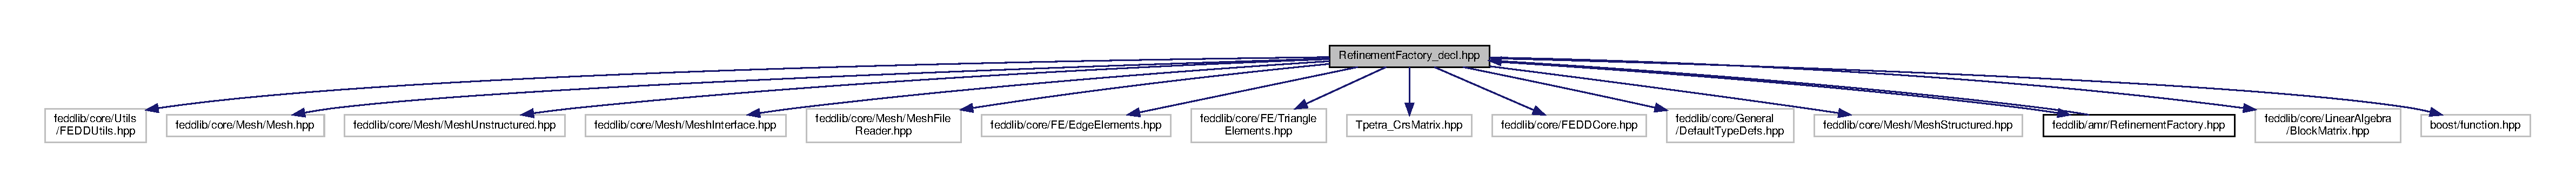
\includegraphics[width=350pt]{RefinementFactory__decl_8hpp__incl}
\end{center}
\end{figure}
This graph shows which files directly or indirectly include this file\+:
\nopagebreak
\begin{figure}[H]
\begin{center}
\leavevmode
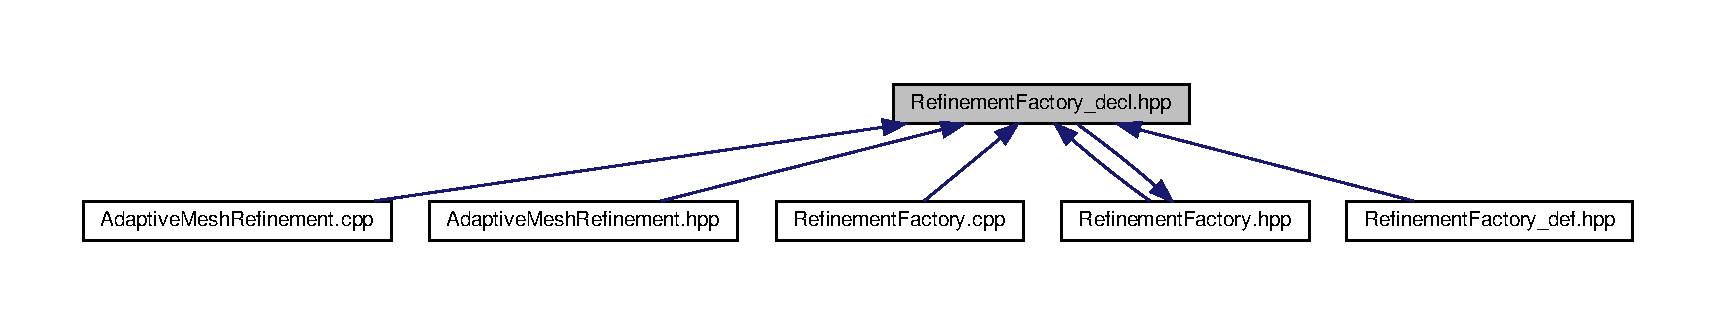
\includegraphics[width=350pt]{RefinementFactory__decl_8hpp__dep__incl}
\end{center}
\end{figure}
\subsection*{Data Structures}
\begin{DoxyCompactItemize}
\item 
class \hyperlink{classFEDD_1_1RefinementFactory}{F\+E\+D\+D\+::\+Refinement\+Factory$<$ S\+C, L\+O, G\+O, N\+O $>$}
\end{DoxyCompactItemize}
\subsection*{Namespaces}
\begin{DoxyCompactItemize}
\item 
 \hyperlink{namespaceFEDD}{F\+E\+DD}
\begin{DoxyCompactList}\small\item\em Mesh\+Unstructured\+Refinement. \end{DoxyCompactList}\end{DoxyCompactItemize}

\hypertarget{RefinementFactory__def_8hpp}{}\section{Refinement\+Factory\+\_\+def.\+hpp File Reference}
\label{RefinementFactory__def_8hpp}\index{Refinement\+Factory\+\_\+def.\+hpp@{Refinement\+Factory\+\_\+def.\+hpp}}
{\ttfamily \#include \char`\"{}Refinement\+Factory\+\_\+decl.\+hpp\char`\"{}}\newline
{\ttfamily \#include \char`\"{}feddlib/core/\+Linear\+Algebra/\+Multi\+Vector\+\_\+def.\+hpp\char`\"{}}\newline
{\ttfamily \#include $<$chrono$>$}\newline
Include dependency graph for Refinement\+Factory\+\_\+def.\+hpp\+:\nopagebreak
\begin{figure}[H]
\begin{center}
\leavevmode
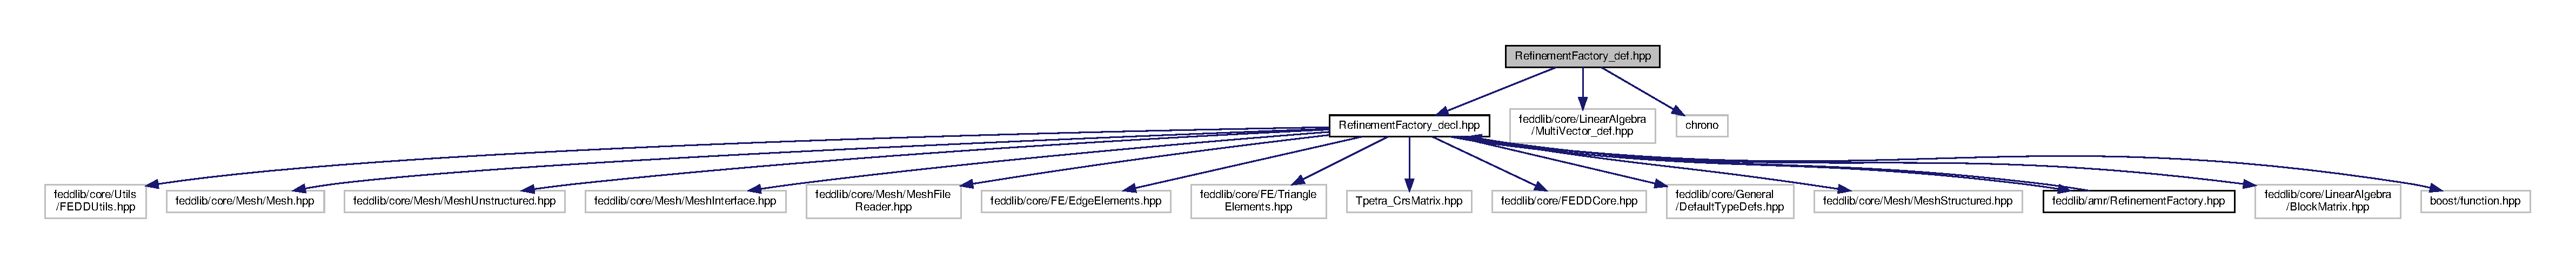
\includegraphics[width=350pt]{RefinementFactory__def_8hpp__incl}
\end{center}
\end{figure}
\subsection*{Namespaces}
\begin{DoxyCompactItemize}
\item 
 \hyperlink{namespaceFEDD}{F\+E\+DD}
\begin{DoxyCompactList}\small\item\em Mesh\+Unstructured\+Refinement. \end{DoxyCompactList}\end{DoxyCompactItemize}
\subsection*{Macros}
\begin{DoxyCompactItemize}
\item 
\#define \hyperlink{RefinementFactory__def_8hpp_aa1a5c1388eec07e84b71fa4f0f534bda}{M\+E\+S\+H\+\_\+\+T\+I\+M\+E\+R\+\_\+\+S\+T\+A\+RT}(A,  S)~Teuchos\+::\+R\+CP$<$Teuchos\+::\+Time\+Monitor$>$ A = Teuchos\+::rcp(new Teuchos\+::\+Time\+Monitor($\ast$Teuchos\+::\+Time\+Monitor\+::get\+New\+Timer(std\+::string(\char`\"{}Mesh Refinement\char`\"{}) + std\+::string(S))));
\item 
\#define \hyperlink{RefinementFactory__def_8hpp_a3c920e3d75aa84a024c9750ea98dd8a0}{M\+E\+S\+H\+\_\+\+T\+I\+M\+E\+R\+\_\+\+S\+T\+OP}(A)~A.\+reset();
\end{DoxyCompactItemize}


\subsection{Macro Definition Documentation}
\mbox{\Hypertarget{RefinementFactory__def_8hpp_aa1a5c1388eec07e84b71fa4f0f534bda}\label{RefinementFactory__def_8hpp_aa1a5c1388eec07e84b71fa4f0f534bda}} 
\index{Refinement\+Factory\+\_\+def.\+hpp@{Refinement\+Factory\+\_\+def.\+hpp}!M\+E\+S\+H\+\_\+\+T\+I\+M\+E\+R\+\_\+\+S\+T\+A\+RT@{M\+E\+S\+H\+\_\+\+T\+I\+M\+E\+R\+\_\+\+S\+T\+A\+RT}}
\index{M\+E\+S\+H\+\_\+\+T\+I\+M\+E\+R\+\_\+\+S\+T\+A\+RT@{M\+E\+S\+H\+\_\+\+T\+I\+M\+E\+R\+\_\+\+S\+T\+A\+RT}!Refinement\+Factory\+\_\+def.\+hpp@{Refinement\+Factory\+\_\+def.\+hpp}}
\subsubsection{\texorpdfstring{M\+E\+S\+H\+\_\+\+T\+I\+M\+E\+R\+\_\+\+S\+T\+A\+RT}{MESH\_TIMER\_START}}
{\footnotesize\ttfamily \#define M\+E\+S\+H\+\_\+\+T\+I\+M\+E\+R\+\_\+\+S\+T\+A\+RT(\begin{DoxyParamCaption}\item[{}]{A,  }\item[{}]{S }\end{DoxyParamCaption})~Teuchos\+::\+R\+CP$<$Teuchos\+::\+Time\+Monitor$>$ A = Teuchos\+::rcp(new Teuchos\+::\+Time\+Monitor($\ast$Teuchos\+::\+Time\+Monitor\+::get\+New\+Timer(std\+::string(\char`\"{}Mesh Refinement\char`\"{}) + std\+::string(S))));}

\mbox{\Hypertarget{RefinementFactory__def_8hpp_a3c920e3d75aa84a024c9750ea98dd8a0}\label{RefinementFactory__def_8hpp_a3c920e3d75aa84a024c9750ea98dd8a0}} 
\index{Refinement\+Factory\+\_\+def.\+hpp@{Refinement\+Factory\+\_\+def.\+hpp}!M\+E\+S\+H\+\_\+\+T\+I\+M\+E\+R\+\_\+\+S\+T\+OP@{M\+E\+S\+H\+\_\+\+T\+I\+M\+E\+R\+\_\+\+S\+T\+OP}}
\index{M\+E\+S\+H\+\_\+\+T\+I\+M\+E\+R\+\_\+\+S\+T\+OP@{M\+E\+S\+H\+\_\+\+T\+I\+M\+E\+R\+\_\+\+S\+T\+OP}!Refinement\+Factory\+\_\+def.\+hpp@{Refinement\+Factory\+\_\+def.\+hpp}}
\subsubsection{\texorpdfstring{M\+E\+S\+H\+\_\+\+T\+I\+M\+E\+R\+\_\+\+S\+T\+OP}{MESH\_TIMER\_STOP}}
{\footnotesize\ttfamily \#define M\+E\+S\+H\+\_\+\+T\+I\+M\+E\+R\+\_\+\+S\+T\+OP(\begin{DoxyParamCaption}\item[{}]{A }\end{DoxyParamCaption})~A.\+reset();}


%--- End generated contents ---

% Index
\backmatter
\newpage
\phantomsection
\clearemptydoublepage
\addcontentsline{toc}{chapter}{Index}
\printindex

\end{document}
